%!TEX encoding = UTF-8 Unicode

\documentclass [a4paper, 11pt] {book}

%-----------------------------------------------------------------------------------------------------------------------*
%                                                                                                                       *
%   « N O I R    E T    B L A N C »    O U    « C O U L E U R »                                                         *
%                                                                                                                       *
%-----------------------------------------------------------------------------------------------------------------------*

%--- Par défaut, l'impression se fait en couleur
\providecommand{\sortieEnCouleur}{true}

%-----------------------------------------------------------------------------------------------------------------------*
%                                                                                                                       *
%   R É G L A G E S    « F R A N Ç A I S »                                                                              *
%                                                                                                                       *
%-----------------------------------------------------------------------------------------------------------------------*

%--- Paquetage pour imposer les réglages français
\usepackage[francais]{babel}

%-----------------------------------------------------------------------------------------------------------------------*
%                                                                                                                       *
%   E N C O D A G E    D E S    S O U R C E S     :     U T F 8                                                         *
%                                                                                                                       *
%-----------------------------------------------------------------------------------------------------------------------*

%--- Paquetage pour le codage des sources en UTF-8
\usepackage[utf8]{inputenc}

%--- Latex demande ce paquetage pour mieux afficher le caractère "°" et \textquotesingle "'"
\usepackage{textcomp}

%--- Ce paquetage permet d'effectuer certaines césures, et ainsi d'éviter les messages "Overfull \hbox"
\usepackage[T1]{fontenc}

%-----------------------------------------------------------------------------------------------------------------------*
%                                                                                                                       *
%   M I S E    E N    P A G E S                                                                                         *
%                                                                                                                       *
%-----------------------------------------------------------------------------------------------------------------------*

% Voir "Une courte introduction à Latex2e", § 6.4

%--- Marge gauche : 2,8 cm ; le paramètre \hoffset contient cette valeur, moins 1 pouce
%    \hoffset = 2,8 cm - 2,54 cm = 0,26 cm
\setlength{\hoffset}{0.26 cm}

%--- Marges supplémentaires, différenciées pour les pages gauches et droites ; ici, aucune.
\setlength{\oddsidemargin }{0 cm}
\setlength{\evensidemargin}{0 cm}

%--- Largeur du texte
%    \textwidth = 210 mm - 28 mm - 28 mm = 15,4 cm
\setlength{\textwidth}{15.4 cm}

%--- Marge haute : 2,8 cm ; le paramètre \voffset contient cette valeur, moins 1 pouce
%    \voffset = 2,8 cm - 2,54 cm = 0,26 cm
\setlength{\voffset}{0.26 cm}

%--- Distance entre la marge haute et l'en-tête : 0 cm
\setlength{\topmargin}{0 cm}

%--- Hauteur de l'en-tête de chaque page : 1 cm
\setlength{\headheight}{1 cm}

%--- Distance entre l'en-tête de chaque page et le corps : 0,5 cm
\setlength{\headsep}{0.5 cm}

%--- Hauteur du corps
%    \textheight = 29,7 cm - 2,8 cm - 2,8 cm - 1,5 cm = 22,6 cm
\setlength{\textheight}{22.6 cm}

%-----------------------------------------------------------------------------------------------------------------------*
%                                                                                                                       *
%   C H O I X    D E    L A    P O L I C E                                                                              *
%                                                                                                                       *
%-----------------------------------------------------------------------------------------------------------------------*

% http://www.cuk.ch/articles/4237
% Un seul des choix suivants doit être validé ; si aucun, c'est la police par défaut qui est utilisée

%---------------------------------------------------- Pour utiliser la police "Times"
%\renewcommand{\rmdefault}{ptm}
%\usepackage{mathptmx}

%---------------------------------------------------- Pour utiliser la police "Palatino"
%\renewcommand{\rmdefault}{ppl}
%\usepackage{mathpazo}

%---------------------------------------------------- Pour utiliser la police "Bookman"
%\usepackage{bookman}

%---------------------------------------------------- Pour utiliser la police "Fourier"
\usepackage{fouriernc}
\usepackage[scaled=0.875]{helvet}
%\usepackage{courier}

%---------------------------------------------------- Pour utiliser la police "Beton, euler"
%\usepackage{beton, euler}

%---------------------------------------------------- Pour utiliser la police "Utopia - MathDesign"
%\usepackage[utopia]{mathdesign}

%---------------------------------------------------- Pour utiliser la police "Charter - MathDesign"
%\usepackage[charter]{mathdesign}

%-----------------------------------------------------------------------------------------------------------------------*
%                                                                                                                       *
%   E X T E N S I O N S    P O U R    L ' É C R I T U R E    D E S     F O R M U L E S    M A T H É M A T I Q U E S     *
%                                                                                                                       *
%-----------------------------------------------------------------------------------------------------------------------*

%--- Extensions pour l'écriture des formules mathématiques
\usepackage{amsmath}
\usepackage{amssymb}
\usepackage{amsfonts}

%--- Paquetage "IEEEtrantools"
% Pour créer des tableaux d'équations, bien alignées
% Voir courte-intro-latex.pdf, page §3.5.2 page 83
\usepackage[retainorgcmds]{IEEEtrantools}


%-----------------------------------------------------------------------------------------------------------------------*
%                                                                                                                       *
%   P A Q U E T A G E    « I F T H E N »                                                                                *
%                                                                                                                       *
%-----------------------------------------------------------------------------------------------------------------------*

%--- Ce paquetage permet d'effectuer des tests : \ifthenelse{test}{bloc then}{bloc else}
\usepackage{ifthen}

%-----------------------------------------------------------------------------------------------------------------------*
%                                                                                                                       *
%   E X T E N S I O N S    P O U R    P R É S E N T E R    L E S    T A B L E A U X                                     *
%                                                                                                                       *
%-----------------------------------------------------------------------------------------------------------------------*

\usepackage{array}
\usepackage[table]{xcolor} % À placer avant \usepackage{listings}

%\renewcommand{\arraystretch}{1.2}

%--- Couleur de fond alternée des tableaux
\ifthenelse{\equal{\sortieEnCouleur}{true}}{
  \newcommand\fondTableau{yellow!25}
}{
  \newcommand\fondTableau{gray!25}
}


%--- Ce paquetage permet de changer le style des légendes des tableaux et des figures (voir caption-eng.pdf) :
%  - l'étiquette est en italique gras
%  - le titre est en italique.
\usepackage[font=it, labelfont=bf]{caption}

%--- Par défaut, le paquetage nomme "Table" les tableaux. La commande
%   suivante impose le nom "Tableau"
% Voir http://fr.wikibooks.org/wiki/LaTeX/Éléments_flottants_et_figures
\addto\captionsfrench{\def\tablename{Tableau}}

%------------------------------------------------------------------------------------------ RÉFÉRENCES À UN TABLEAU
% La référence au tableau "nom-du-tableau" est définie par \labelTableau{nom-du-tableau}
\newcommand\labelTableau[1]{\label{tab:#1}}
% Latex autorise deux types d'appel à une référence \ref{tab:nom-du-tableau} et \pageref{tab:nom-du-tableau}

% \refTableau{}{nom-du-tableau} ---> "tableau x.y"   où x.y est le n° du tableau
\newcommand\refTableau[1]{\hyperref[tab:#1]{tableau \ref*{tab:#1}}}

% \refTableauSansPrefixe{}{nom-du-tableau} ---> "x.y"   où x.y est le n° du tableau
\newcommand\refTableauSansPrefixe[1]{\hyperref[tab:#1]{\ref*{tab:#1}}}

% \refTableauPage{}{nom-du-tableau} ---> "tableau x.y page n"   où x.y est le n° du tableau
\newcommand\refTableauPage[1]{\hyperref[tab:#1]{tableau \ref*{tab:#1} page \pageref{tab:#1}}}

% \refTableauPageSansPrefixe{}{nom-du-tableau} ---> "x.y page n"   où x.y est le n° du tableau
\newcommand\refTableauPageSansPrefixe[1]{\hyperref[tab:#1]{\ref*{tab:#1} page \pageref{tab:#1}}}

%-----------------------------------------------------------------------------------------------------------------------*
%                                                                                                                       *
%   P A Q U E T A G E    « L I S T I N G S »                                                                            *
%                                                                                                                       *
%-----------------------------------------------------------------------------------------------------------------------*

\usepackage{listings} % À placer après \usepackage[table]{xcolor}

%-----------------------------------------------------------------------------------------------------------------------*
%                                                                                                                       *
%   T I K Z    -    P G F                                                                                               *
%                                                                                                                       *
%-----------------------------------------------------------------------------------------------------------------------*

\usepackage{tikz}
\usetikzlibrary{calc}
\usepackage{pgfplots}
\usetikzlibrary{arrows}
\usetikzlibrary{decorations}
\usetikzlibrary{decorations.pathmorphing}
\usetikzlibrary{shapes.callouts}
\usetikzlibrary{automata}
\usetikzlibrary{positioning}
\usepgflibrary{shapes.geometric}

%-----------------------------------------------------------------------------------------------------------------------*
%                                                                                                                       *
%   T E X T E    E N C E R C L É                                                                                        *
%                                                                                                                       *
%-----------------------------------------------------------------------------------------------------------------------*

%\newcommand\texteEncercle[1]{\tikz \node[draw,circle, inner sep=0.5, text height=2mm]{#1}}
\newcommand\texteEncercle[1]{#1}

%-----------------------------------------------------------------------------------------------------------------------*
%                                                                                                                       *
%   I N C L U S I O N    D E S   M A C R O S   D E S T I N É E S   À   L ' É C R I T U R E   
%                                                                                                                       *
%                                        D E   C O D E   G A L G A S                                                    *
%                                                                                                                       *
%-----------------------------------------------------------------------------------------------------------------------*

\usepackage{relsize}

%!TEX encoding = UTF-8 Unicode
%!TEX root = ../galgas-book.tex

%-----------------------------------------------------------------------------------------------------------------------*
%   A F F I C H A G E    D U    C O D E    S H E L L                                                                    *
%-----------------------------------------------------------------------------------------------------------------------*

\newcommand\tpp[1]{\colorbox{gray!12}{\ttfamily #1}}

\makeatletter
\newcommand{\zeroEspaceAvantPonctuation}[1]{\nofrench@punctuation{#1}\french@punctuation}
\makeatother

%-----------------------------------------------------------------------------------------------------------------------*
%   A F F I C H A G E    D U    C O D E    G A L G A S                                                                  *
%-----------------------------------------------------------------------------------------------------------------------*

% http://latexcolor.com

\definecolor{modebeige}{rgb}{0.59, 0.44, 0.09}

\newcommand\keywordsStyleGalgas[1]{\textcolor{blue}{\textbf{#1}}}
\newcommand\delimitersStyleGalgas[1]{\textcolor{brown}{\textbf{#1}}}
\newcommand\selectorStyleGalgas[1]{\textcolor{PineGreen}{#1}}
\newcommand\terminalStyleGalgas[1]{\textcolor{orange}{#1}}
\newcommand\nonTerminalStyleGalgas[1]{\textcolor{orange}{#1}}
\newcommand\integerStyleGalgas[1]{\textcolor{Mulberry}{#1}}
\newcommand\bigintStyleGalgas[1]{\textcolor{modebeige}{#1}}
\newcommand\floatStyleGalgas[1]{\textcolor{magenta}{#1}}
\newcommand\characterStyleGalgas[1]{\textcolor{cyan}{#1}}
\newcommand\stringStyleGalgas[1]{\textcolor{gray}{#1}}
\newcommand\typeNameStyleGalgas[1]{\textcolor{gray}{#1}}
\newcommand\attributeStyleGalgas[1]{\textcolor{brown}{#1}}
\newcommand\commentStyleGalgas[1]{\textcolor{red}{#1}}

\newcommand\lexicalErrorGalgas{\textcolor{red}{\textbullet ERRLEX\textbullet}}

\newcommand\keywordsStylegalgas[1]{\textcolor{blue}{\textbf{#1}}}
\newcommand\delimitersStylegalgas[1]{\textcolor{brown}{\textbf{#1}}}
\newcommand\selectorStylegalgas[1]{\textcolor{PineGreen}{#1}}
\newcommand\terminalStylegalgas[1]{\textcolor{orange}{#1}}
\newcommand\nonTerminalStylegalgas[1]{\textcolor{orange}{#1}}
\newcommand\integerStylegalgas[1]{\textcolor{Mulberry}{#1}}
\newcommand\bigintStylegalgas[1]{\textcolor{modebeige}{#1}}
\newcommand\floatStylegalgas[1]{\textcolor{magenta}{#1}}
\newcommand\characterStylegalgas[1]{\textcolor{cyan}{#1}}
\newcommand\stringStylegalgas[1]{\textcolor{gray}{#1}}
\newcommand\typeNameStylegalgas[1]{\textcolor{gray}{#1}}
\newcommand\attributeStylegalgas[1]{\textcolor{brown}{#1}}
\newcommand\commentStylegalgas[1]{\textcolor{red}{#1}}

\newcommand\lexicalErrorgalgas{\textcolor{red}{\textbullet ERRLEX\textbullet}}

\newwrite\tempfile

%-----------------------------------------------------------------------------------------------------------------------*
% ENVIRONNEMENT galgas3 : affichage de code galgas 3
%-----------------------------------------------------------------------------------------------------------------------*

\newmdenv[
  topline=false,
  bottomline=false,
  rightline=false,
  skipabove=0pt,
  skipbelow=0pt,
  linecolor=orange!50,
  backgroundcolor=gray!5,
  linewidth=1pt,
  frametitle={GALGAS 3},
  frametitlefont=\normalfont\bfseries\scriptsize,
  frametitlerule=true,
  frametitleaboveskip=3pt,
  frametitlebelowskip=3pt,
]{siderules3}

\makeatletter
\newenvironment{galgas3}{%
  \begingroup
  \@bsphack
  \immediate\openout\tempfile=temp.galgas%
  \let\do\@makeother\dospecials
  \catcode`\^^M\active
  \verbatim@startline
  \verbatim@addtoline
  \verbatim@finish
  \def\verbatim@processline{\immediate\write\tempfile{\the\verbatim@line}}%
  \verbatim@start
}{
  \immediate\closeout\tempfile
  \@esphack
  \endgroup
  \immediate\write18{galgas -q --mode=latex:Galgas temp.galgas}
  {\medskip\begin{siderules3}\zeroEspaceAvantPonctuation{\tt{\keywordsStyleGalgas{r{}u{}l{}e{}}\hspace*{.6em}\nonTerminalStyleGalgas{\textless{}T{}\textgreater{}}\hspace*{.6em}\delimitersStyleGalgas{\{}\hspace*{.6em}I{}1{}\hspace*{.6em}I{}0{}\hspace*{.6em}\nonTerminalStyleGalgas{\textless{}T{}\textgreater{}}\hspace*{.6em}\delimitersStyleGalgas{\}}\newline
\newline
\keywordsStyleGalgas{r{}u{}l{}e{}}\hspace*{.6em}\nonTerminalStyleGalgas{\textless{}T{}\textgreater{}}\hspace*{.6em}\delimitersStyleGalgas{\{}\hspace*{.6em}I{}2{}\hspace*{.6em}I{}0{}\hspace*{.6em}\nonTerminalStyleGalgas{\textless{}T{}\textgreater{}}\hspace*{.6em}\delimitersStyleGalgas{\}}\newline
\newline
\keywordsStyleGalgas{r{}u{}l{}e{}}\hspace*{.6em}\nonTerminalStyleGalgas{\textless{}T{}\textgreater{}}\hspace*{.6em}\delimitersStyleGalgas{\{}\hspace*{.6em}\hspace*{.6em}\delimitersStyleGalgas{\}}}}\end{siderules3}}
}
\makeatother

%-----------------------------------------------------------------------------------------------------------------------*
% ENVIRONNEMENT galgas3box : affichage de code galgas encadré                                                           *
%-----------------------------------------------------------------------------------------------------------------------*

\newmdenv[
  skipabove=0pt,
  skipbelow=0pt,
  linecolor=orange!25,
  backgroundcolor=gray!5,
  linewidth=1pt,
  frametitle={GALGAS 3},
  frametitlefont=\normalfont\bfseries\scriptsize,
  frametitlerule=true,
  frametitleaboveskip=3pt,
  frametitlebelowskip=3pt,
]{boxrules3}

%-----------------------------------------------------------------------------------------------------------------------*

\makeatletter
\newenvironment{galgas3box}{%
  \begingroup
  \@bsphack
  \immediate\openout\tempfile=temp.galgas%
  \let\do\@makeother\dospecials
  \catcode`\^^M\active
  \verbatim@startline
  \verbatim@addtoline
  \verbatim@finish
  \def\verbatim@processline{\immediate\write\tempfile{\the\verbatim@line}}%
  \verbatim@start
}{
  \immediate\closeout\tempfile
  \@esphack
  \endgroup
  \immediate\write18{galgas -q --mode=latex:Galgas temp.galgas}
  {\singlespacing\begin{boxrules3}\zeroEspaceAvantPonctuation{\tt{\keywordsStyleGalgas{r{}u{}l{}e{}}\hspace*{.6em}\nonTerminalStyleGalgas{\textless{}T{}\textgreater{}}\hspace*{.6em}\delimitersStyleGalgas{\{}\hspace*{.6em}I{}1{}\hspace*{.6em}I{}0{}\hspace*{.6em}\nonTerminalStyleGalgas{\textless{}T{}\textgreater{}}\hspace*{.6em}\delimitersStyleGalgas{\}}\newline
\newline
\keywordsStyleGalgas{r{}u{}l{}e{}}\hspace*{.6em}\nonTerminalStyleGalgas{\textless{}T{}\textgreater{}}\hspace*{.6em}\delimitersStyleGalgas{\{}\hspace*{.6em}I{}2{}\hspace*{.6em}I{}0{}\hspace*{.6em}\nonTerminalStyleGalgas{\textless{}T{}\textgreater{}}\hspace*{.6em}\delimitersStyleGalgas{\}}\newline
\newline
\keywordsStyleGalgas{r{}u{}l{}e{}}\hspace*{.6em}\nonTerminalStyleGalgas{\textless{}T{}\textgreater{}}\hspace*{.6em}\delimitersStyleGalgas{\{}\hspace*{.6em}\hspace*{.6em}\delimitersStyleGalgas{\}}}}\end{boxrules3}}
}
\makeatother

%-----------------------------------------------------------------------------------------------------------------------*
% COMMANDE \ggst : affichage de code en ligne galgas 3
%-----------------------------------------------------------------------------------------------------------------------*

\makeatletter
\newcommand*\ggst{%
  \@bsphack%
  \begingroup%
  \let\do\@makeother\dospecials%
  \let\do\do@noligs\verbatim@nolig@list%
  \catcode`\^^M=15\relax%
  \@vobeyspaces%
  \@ggst{\temporary}%
}%
\newcommand\@ggst[2]{%
  \catcode`-=12\relax%
  \catcode`<=12\relax%
  \catcode`>=12\relax%
  \catcode`,=12\relax%
  \catcode`'=12\relax%
  \catcode``=12\relax%
  \catcode`#2\active%
  \catcode`~\active%
  \lccode`\~`#2\relax%
  \begingroup%
  \lowercase{%
    \def\@tempa##1~{%
      \expandafter\endgroup%
      \expandafter\DeclareRobustCommand%
      \expandafter*%
      \expandafter#1%
      \expandafter{\@tempa}%
      \@esphack%
      \immediate\openout\tempfile=temp.galgas%
      \immediate\write\tempfile{##1}%
      \immediate\closeout\tempfile%
      \immediate\write18{galgas -q --mode=latex:Galgas temp.galgas}%
      \colorbox{gray!6}{\zeroEspaceAvantPonctuation{\tt{\keywordsStyleGalgas{r{}u{}l{}e{}}\hspace*{.6em}\nonTerminalStyleGalgas{\textless{}T{}\textgreater{}}\hspace*{.6em}\delimitersStyleGalgas{\{}\hspace*{.6em}I{}1{}\hspace*{.6em}I{}0{}\hspace*{.6em}\nonTerminalStyleGalgas{\textless{}T{}\textgreater{}}\hspace*{.6em}\delimitersStyleGalgas{\}}\newline
\newline
\keywordsStyleGalgas{r{}u{}l{}e{}}\hspace*{.6em}\nonTerminalStyleGalgas{\textless{}T{}\textgreater{}}\hspace*{.6em}\delimitersStyleGalgas{\{}\hspace*{.6em}I{}2{}\hspace*{.6em}I{}0{}\hspace*{.6em}\nonTerminalStyleGalgas{\textless{}T{}\textgreater{}}\hspace*{.6em}\delimitersStyleGalgas{\}}\newline
\newline
\keywordsStyleGalgas{r{}u{}l{}e{}}\hspace*{.6em}\nonTerminalStyleGalgas{\textless{}T{}\textgreater{}}\hspace*{.6em}\delimitersStyleGalgas{\{}\hspace*{.6em}\hspace*{.6em}\delimitersStyleGalgas{\}}}}\unskip}%
    }%
  }%
  \ifnum`#2=`\~\else\@makeother\~\fi%
  \expandafter\endgroup%
  \@tempa%
}%
\makeatother

%-----------------------------------------------------------------------------------------------------------------------*
% ENVIRONNEMENT galgas4 : affichage de code galgas 4
%-----------------------------------------------------------------------------------------------------------------------*


\newmdenv[
  topline=false,
  bottomline=false,
  rightline=false,
  skipabove=0pt,
  skipbelow=0pt,
  linecolor=blue,
  backgroundcolor=gray!5,
  linewidth=1pt,
  frametitle={GALGAS 4},
  frametitlefont=\normalfont\bfseries\scriptsize,
  frametitlerule=true,
  frametitleaboveskip=3pt,
  frametitlebelowskip=3pt,
]{siderules4}

\makeatletter
\newenvironment{galgas4}{%
  \begingroup
  \@bsphack
  \immediate\openout\tempfile=temp.ggs%
  \let\do\@makeother\dospecials
  \catcode`\^^M\active
  \verbatim@startline
  \verbatim@addtoline
  \verbatim@finish
  \def\verbatim@processline{\immediate\write\tempfile{\the\verbatim@line}}%
  \verbatim@start
}{
  \immediate\closeout\tempfile
  \@esphack
  \endgroup
  \immediate\write18{galgas -q --mode=latex:Galgas temp.ggs}
  {\medskip\begin{siderules4}\zeroEspaceAvantPonctuation{\tt{\attributeStyleGalgas{\%r{}e{}m{}o{}v{}e{}S{}e{}t{}t{}e{}r{}}\hspace*{.6em}n{}o{}m{}\hspace*{.6em}\attributeStyleGalgas{\%e{}r{}r{}o{}r{}M{}e{}s{}s{}a{}g{}e{}}\hspace*{.6em}\stringStyleGalgas{"m{}e{}s{}s{}a{}g{}e{}\_e{}r{}r{}e{}u{}r{}"}}}\end{siderules4}}
}
\makeatother

%-----------------------------------------------------------------------------------------------------------------------*
% ENVIRONNEMENT galgas34 : affichage de code galgas 3 et galgas4
%-----------------------------------------------------------------------------------------------------------------------*


\newmdenv[
  topline=false,
  bottomline=false,
  rightline=false,
  skipabove=0pt,
  skipbelow=0pt,
  linecolor=green,
  backgroundcolor=gray!5,
  linewidth=1pt,
  frametitle={GALGAS 3 et GALGAS 4},
  frametitlefont=\normalfont\bfseries\scriptsize,
  frametitlerule=true,
  frametitleaboveskip=3pt,
  frametitlebelowskip=3pt,
]{siderules34}

\makeatletter
\newenvironment{galgas34}{%
  \begingroup
  \@bsphack
  \immediate\openout\tempfile=temp.ggs%
  \let\do\@makeother\dospecials
  \catcode`\^^M\active
  \verbatim@startline
  \verbatim@addtoline
  \verbatim@finish
  \def\verbatim@processline{\immediate\write\tempfile{\the\verbatim@line}}%
  \verbatim@start
}{
  \immediate\closeout\tempfile
  \@esphack
  \endgroup
  \immediate\write18{galgas -q --mode=latex:Galgas temp.ggs}
  {\medskip\begin{siderules34}\zeroEspaceAvantPonctuation{\tt{\attributeStyleGalgas{\%r{}e{}m{}o{}v{}e{}S{}e{}t{}t{}e{}r{}}\hspace*{.6em}n{}o{}m{}\hspace*{.6em}\attributeStyleGalgas{\%e{}r{}r{}o{}r{}M{}e{}s{}s{}a{}g{}e{}}\hspace*{.6em}\stringStyleGalgas{"m{}e{}s{}s{}a{}g{}e{}\_e{}r{}r{}e{}u{}r{}"}}}\end{siderules34}}
}
\makeatother

%-----------------------------------------------------------------------------------------------------------------------*
% ENVIRONNEMENT galgas4box : affichage de code galgas encadré
%-----------------------------------------------------------------------------------------------------------------------*

\newmdenv[
  skipabove=0pt,
  skipbelow=0pt,
  linecolor=blue,
  backgroundcolor=gray!5,
  linewidth=1pt,
  frametitle={GALGAS 4},
  frametitlefont=\normalfont\bfseries\scriptsize,
  frametitlerule=true,
  frametitleaboveskip=3pt,
  frametitlebelowskip=3pt,
]{boxrules4}

%-----------------------------------------------------------------------------------------------------------------------*

\makeatletter
\newenvironment{galgas4box}{%
  \begingroup
  \@bsphack
  \immediate\openout\tempfile=temp.ggs%
  \let\do\@makeother\dospecials
  \catcode`\^^M\active
  \verbatim@startline
  \verbatim@addtoline
  \verbatim@finish
  \def\verbatim@processline{\immediate\write\tempfile{\the\verbatim@line}}%
  \verbatim@start
}{
  \immediate\closeout\tempfile
  \@esphack
  \endgroup
  \immediate\write18{galgas -q --mode=latex:Galgas temp.ggs}
  {\singlespacing\begin{boxrules4}\zeroEspaceAvantPonctuation{\tt{\attributeStyleGalgas{\%r{}e{}m{}o{}v{}e{}S{}e{}t{}t{}e{}r{}}\hspace*{.6em}n{}o{}m{}\hspace*{.6em}\attributeStyleGalgas{\%e{}r{}r{}o{}r{}M{}e{}s{}s{}a{}g{}e{}}\hspace*{.6em}\stringStyleGalgas{"m{}e{}s{}s{}a{}g{}e{}\_e{}r{}r{}e{}u{}r{}"}}}\end{boxrules4}}
}
\makeatother

%-----------------------------------------------------------------------------------------------------------------------*
% COMMANDE \ggsq : affichage de code en ligne galgas 4
%-----------------------------------------------------------------------------------------------------------------------*

\makeatletter
\newcommand*\ggsq{%
  \@bsphack%
  \begingroup%
  \let\do\@makeother\dospecials%
  \let\do\do@noligs\verbatim@nolig@list%
  \catcode`\^^M=15\relax%
  \@vobeyspaces%
  \@ggsq{\temporary}%
}%
\newcommand\@ggsq[2]{%
  \catcode`-=12\relax%
  \catcode`<=12\relax%
  \catcode`>=12\relax%
  \catcode`,=12\relax%
  \catcode`'=12\relax%
  \catcode``=12\relax%
  \catcode`#2\active%
  \catcode`~\active%
  \lccode`\~`#2\relax%
  \begingroup%
  \lowercase{%
    \def\@tempa##1~{%
      \expandafter\endgroup%
      \expandafter\DeclareRobustCommand%
      \expandafter*%
      \expandafter#1%
      \expandafter{\@tempa}%
      \@esphack%
      \immediate\openout\tempfile=temp.ggs%
      \immediate\write\tempfile{##1}%
      \immediate\closeout\tempfile%
      \immediate\write18{galgas -q --mode=latex:Galgas temp.ggs}%
      \colorbox{gray!6}{\zeroEspaceAvantPonctuation{\tt{\attributeStyleGalgas{\%r{}e{}m{}o{}v{}e{}S{}e{}t{}t{}e{}r{}}\hspace*{.6em}n{}o{}m{}\hspace*{.6em}\attributeStyleGalgas{\%e{}r{}r{}o{}r{}M{}e{}s{}s{}a{}g{}e{}}\hspace*{.6em}\stringStyleGalgas{"m{}e{}s{}s{}a{}g{}e{}\_e{}r{}r{}e{}u{}r{}"}}}\unskip}%
    }%
  }%
  \ifnum`#2=`\~\else\@makeother\~\fi%
  \expandafter\endgroup%
  \@tempa%
}%
\makeatother

%-----------------------------------------------------------------------------------------------------------------------*
%                                                                                                                       *
% A F F I C H A G E    E T    C R O S S   R É F É R E N C E    D E S    T Y P E S    P R É D É F I N I S   G A L G A S  *
%                                                                                                                       *
%-----------------------------------------------------------------------------------------------------------------------*

%--- Les macros suivantes définissent une section et une sous-section :
%      - en formattant le titre
%      - en définissant un label pour cross référence ;
%      - en définissant une entrée dans l'index

% Exemple d'appel : \sectionTypePredefiniLabelIndex{bool}

\newcommand \chapitreTypePredefiniLabelIndex[1] {\chapter{Le type \texttt{@#1}}\label{type:#1}\index{Type!"@#1}}

\newcommand \sectionTypePredefiniLabelIndex[1] {\section{Le type \texttt{@#1}}\label{type:#1}\index{Type!"@#1}}

\newcommand \subsectionTypePredefiniLabelIndex[1] {\subsection{Le type \texttt{@#1}}\label{type:#1}\index{Type!"@#1}}

%--- Cette macro établit un hyperlien vers un type prédéfini
% Exemple d'appel : \refTypePredefini{bool} -- affiche --> @bool type (page xx)

\newcommand \refTypePredefini[1] {\hyperref[type:#1]{\texttt{@#1} (page \pageref{type:#1})}}

%-----------------------------------------------------------------------------------------------------------------------*
%   G E T T E R   C R O S S    R E F E R E N C I N G                                                                    *
%-----------------------------------------------------------------------------------------------------------------------*

\newcommand\sectionGetter[2]{\section{Getter \texttt{#1}}\label{getter:#2:#1}\index{#1!getter "@#2}}

\newcommand\subsectionGetter[2]{\subsection{Getter \texttt{#1}}\label{getter:#2:#1}\index{#1!getter "@#2}}

%-----------------------------------------------------------------------------------------------------------------------*

% Exemple d'appel : \refGetterPage{bool}{string} -- affiche --> @bool string getter (page xx)
\newcommand\refGetterPage[2] {\hyperref[getter:#1:#2]{
  \emph{getter} \texttt{#2} \emph{du type} \texttt{@#1} \emph{(page \pageref{getter:#1:#2})}}
}

%-----------------------------------------------------------------------------------------------------------------------*
%   S E T T E R   C R O S S    R E F E R E N C I N G                                                                    *
%-----------------------------------------------------------------------------------------------------------------------*

\newcommand\subsectionSetter[2]{\subsection{Setter \texttt{#1}}\label{setter:#2:#1}\index{#1!setter "@#2}}

%-----------------------------------------------------------------------------------------------------------------------*

% Exemple d'appel : \refSetterPage{bool}{string} -- affiche --> @bool string setter (page xx)
\newcommand\refSetterPage[2] {\hyperref[setter:#1:#2]{
  \emph{setter} \texttt{#2} \emph{du type} \texttt{@#1} \emph{(page \pageref{setter:#1:#2})}}
}


%-----------------------------------------------------------------------------------------------------------------------*
%   M E T H O D   C R O S S    R E F E R E N C I N G                                                                    *
%-----------------------------------------------------------------------------------------------------------------------*

\newcommand\subsectionMethod[2]{\subsection{Méthode \texttt{#1}}\label{method:#2:#1}\index{#1!méthode "@#2}}

%-----------------------------------------------------------------------------------------------------------------------*

% Exemple d'appel : \refSetterPage{bool}{string} -- affiche --> @bool string setter (page xx)
\newcommand\refMethodPage[2] {\hyperref[setter:#1:#2]{
  \emph{méthode} \texttt{#2} \emph{du type} \texttt{@#1} \emph{(page \pageref{method:#1:#2})}}
}


%-----------------------------------------------------------------------------------------------------------------------*
%   C O N S T R U C T O R   C R O S S    R E F E R E N C I N G                                                          *
%-----------------------------------------------------------------------------------------------------------------------*

\newcommand\sectionConstructor[2]{\section{Constructeur \texttt{#1}}\label{constructor:#1:#2}\index{#1!constructeur "@#2}}

\newcommand\subsectionConstructor[2]{\subsection{Constructeur \texttt{#1}}\label{constructor:#1:#2}\index{#1!constructeur "@#2}}

%-----------------------------------------------------------------------------------------------------------------------*

\newcommand \refConstructorPage[2] {\hyperref[constructor:#2:#1]{\em constructeur \texttt{#2} du type \texttt{@#1} -- page \pageref{constructor:#2:#1}}}

%-----------------------------------------------------------------------------------------------------------------------*
%   S T A T I C    P R O C   C R O S S    R E F E R E N C I N G                                                     *
%-----------------------------------------------------------------------------------------------------------------------*

\newcommand\sectionStaticProc[2]{\section{Procédure de type \texttt{#1}}\label{staticProc:#2:#1}\index{#1!"@#2 procédure de type}}

\newcommand\subsectionStaticProc[2]{\subsection{Procédure de type \texttt{#1}}\label{staticProc:#2:#1}\index{#1!"@#2 procédure de type}}

%-----------------------------------------------------------------------------------------------------------------------*

\newcommand \refStaticProcPage[2] {\hyperref[staticProc:#1:#2]{\em procédure \texttt{#2} du type \texttt{@#1} (page \pageref{staticProc:#1:#2})}}

%-----------------------------------------------------------------------------------------------------------------------*


%-----------------------------------------------------------------------------------------------------------------------*
%                                                                                                                       *
%   P A Q U E T A G E    « L O N G T A B L E »                                                                          *
%                                                                                                                       *
%-----------------------------------------------------------------------------------------------------------------------*

%--- Pour afficher correctement des tables sur plusieurs pages
%\usepackage{longtable}

%-----------------------------------------------------------------------------------------------------------------------*
%                                                                                                                       *
%   E N - T Ê T E S    E T    P I E D S    D E    P A G E S                                                             *
%                                                                                                                       *
%-----------------------------------------------------------------------------------------------------------------------*

% Grâce au package "fancyhdr"
% voir http://www.exomatik.net/U-Latex/Personnaliser#toc2
%      http://www.trustonme.net/didactels/250.html
\usepackage{fancyhdr}
\pagestyle{fancy}
%--- Numéro de page : à gauche pages paires, à droite pages impaires
\fancyhead[EL,OR]{\thepage}
%--- Nom de chapitre : à droite page paires
\fancyhead[ER]{\leftmark}
%--- Nom de section : à gauche page impaires
\fancyhead[OL]{\rightmark}
%--- Version GALGAS : au milieu du pied de chaque page
\fancyfoot[C]{GALGAS, version GALGASCURRENTVERSION}
%--- filet en haut et en bas de chaque page
\renewcommand{\headrulewidth}{0.5 pt}
\renewcommand{\footrulewidth}{0.5 pt}

\renewcommand{\chaptermark}[1]{\markboth{\bsc{\chaptername~\thechapter{}.} #1}{}}
\renewcommand{\sectionmark}[1]{\markright{\bsc{\thesection{}.} #1}{}}

%-----------------------------------------------------------------------------------------------------------------------*
%                                                                                                                       *
%   G E S T I O N    D E    L ' I N D E X                                                                               *
%                                                                                                                       *
%-----------------------------------------------------------------------------------------------------------------------*

% http://www.cuk.ch/articles/4097
% http://www.tuteurs.ens.fr/logiciels/latex/makeindex.html
% http://linux.die.net/man/1/makeindex
%
% Attention ! Les deux commandes suivantes, ainsi que le \printindex placé plus bas ne
% sont pas suffisants pour construire l'index : il faut utiliser l'utilitaire "makeIndex"
% Voir le fichier de commande "build.command"
\usepackage{makeidx}
\makeindex

%-----------------------------------------------------------------------------------------------------------------------*
%                                                                                                                       *
%   T O C B I D I N D                                                                                                   *
%                                                                                                                       *
%-----------------------------------------------------------------------------------------------------------------------*

%    Pour faire figurer la liste des tableaux (et la table des matières)
%    dans la table des matières
\usepackage{tocbibind}

\setcounter{tocdepth}{3}

%\titlespacing{\chapter} {0pt} {*0} {*0} {}
%\titlespacing{\section} {4ex} {*0} {*0} {}
%\titlespacing{\subsection} {10ex} {*0} {*0} {}
%\titlespacing{\subsubsection} {\subsubsectskip} {*0} {*0} {}

%\setlength{\parindent}{50pt}
%\makeatletter
%\renewcommand\paragraph{\@startsection{paragraph}{4}{\z@}%
%                                    {3.25ex \@plus 1ex \@minus .2ex}%
%                                    {2.3ex \ at plus.2ex}%
%                                    {\normalfont\normalsize\bfseries}}
%\makeatother

%-----------------------------------------------------------------------------------------------------------------------*
%                                                                                                                       *
%   H Y P E R R E F                                                                                                     *
%                                                                                                                       *
%-----------------------------------------------------------------------------------------------------------------------*

%--- Pour les hyperliens, et le contrôle de la génération PDF 
\usepackage{hyperref}
\hypersetup{colorlinks=true}
\ifthenelse{\equal{\sortieEnCouleur}{true}}{
  \hypersetup{linkcolor=blue}
}{
  \hypersetup{linkcolor=black}
}
\hypersetup{breaklinks=true}

%-----------------------------------------------------------------------------------------------------------------------*
%                                                                                                                       *
%   R É F É R N C E S                                                                                                   *
%                                                                                                                       *
%-----------------------------------------------------------------------------------------------------------------------*

% Au lieu d'écrire \chapter{titre-chapitre}, on écrit \chapterLabel{titre-chapitre}{label-chapitre}
\newcommand \chapterLabel[2]{\chapter{#1}\label{chapter:#2}}

% \refChapter{label-chapter} ---> "chapitre n"
\newcommand \refChapter[1]{\hyperref[chapter:#1]{chapitre \ref*{chapter:#1}}}

\newcommand \refChapterPage[1]{\hyperref[chapter:#1]{chapitre \ref*{chapter:#1} page \pageref{chapter:#1}}}

% Au lieu d'écrire \section{titre-section}, on écrit \sectionLabel{titre-section}{label-section}
\newcommand \sectionLabel[2]{\section{#1}\label{sec:#2}}


% \refSectionPage{label-section} ---> "section x.y page n"   où x.y est le n° de la section
\newcommand\refSectionPage[1]{\hyperref[sec:#1]{section \ref*{sec:#1} page \pageref{sec:#1}}}

%------------------------------------------------------------------------------------------ RÉFÉRENCES À UNE SUB-SECTION
% Au lieu d'écrire \subsection{titre-section}, on écrit \subsectionLabel{titre-section}{label-section}
\newcommand \subsectionLabel[2]{\subsection{#1}\label{subsec:#2}}


% \refSubsectionPage{label-section} ---> "section x.y page n"   où x.y est le n° de la sub-section
\newcommand\refSubsectionPage[1]{\hyperref[subsec:#1]{section \ref*{subsec:#1} page \pageref{subsec:#1}}}

%------------------------------------------------------------------------------------------ RÉFÉRENCES À UNE FIGURE
% La référence au tableau "nom-de-la-figure" est définie par \labelFigure{nom-de-la-figure}
\newcommand\labelFigure[1]{\label{fig:#1}}
% Latex autorise deux types d'appel à une référence \ref{fig:nom-de-la-figure} et \pageref{fig:nom-de-la-figure}

% \refFigure{}{nom-de-la-figure}   ---> "figure x.y"   où x.y est le n° de la figure
% \refFigure{z}{nom-de-la-figure}  ---> "figure x.y.z" où x.y est le n° de la figure
\newcommand\refFigure[2]{\hyperref[fig:#2]{figure \ref*{fig:#2}{\ifthenelse{\equal{#1}{}}{}{.#1}}}}

% \refFigureSansPrefixe{}{nom-de-la-figure}   ---> "x.y"   où x.y est le n° de la figure
% \refFigureSansPrefixe{z}{nom-de-la-figure}  ---> "x.y.z" où x.y est le n° de la figure
\newcommand\refFigureSansPrefixe[2]{\hyperref[fig:#2]{\ref*{fig:#2}{\ifthenelse{\equal{#1}{}}{}{.#1}}}}

% \refFigurePage{}{nom-de-la-figure}   ---> "figure x.y page n"   où x.y est le n° de la figure
% \refFigurePage{z}{nom-de-la-figure}  ---> "figure x.y.z page n" où x.y est le n° de la figure
\newcommand\refFigurePage[2]{\hyperref[fig:#2]{figure \ref*{fig:#2}{\ifthenelse{\equal{#1}{}}{}{.#1}} page \pageref{fig:#2}}}

% \refFigurePageSansPrefixe{}{nom-de-la-figure}   ---> "x.y page n"   où x.y est le n° de la figure
% \refFigurePageSansPrefixe{z}{nom-de-la-figure}  ---> "x.y.z page n" où x.y est le n° de la figure
\newcommand\refFigurePageSansPrefixe[2]{\hyperref[fig:#2]{\ref*{fig:#2}{\ifthenelse{\equal{#1}{}}{}{.#1}} page \pageref{fig:#2}}}

%-----------------------------------------------------------------------------------------------------------------------*
%                                                                                                                       *
%   S H O W K E Y S    ( P O U R    D É B O G U E R )                                                                   *
%                                                                                                                       *
%-----------------------------------------------------------------------------------------------------------------------*

%\usepackage{showkeys}

%-----------------------------------------------------------------------------------------------------------------------*
%                                                                                                                       *
%   T I T L E T O C                                                                                                     *
%                                                                                                                       *
%-----------------------------------------------------------------------------------------------------------------------*

%--- Description dans le paquetage titlesec
% http://forum.mathematex.net/latex-f6/formatage-avance-de-la-table-des-matieres-t11559.html

%\usepackage{titletoc}


%--- Par défaut dans la tables des matières, le numéro de sous-section est trop long et mange le début du titre
%\titlecontents{subsection}[2.5cm]{}{\hspace*{-5.0em}\hyperref[subsection \thecontentslabel]{\thecontentslabel}\hspace*{0.5em}}{}{\titlerule*[0.66pc]{.}\contentspage}{}

%\titlecontents{subsection}[2.5cm]{}{\hspace*{-5.0em}\thecontentslabel\hspace*{0.5em}}{}{\titlerule*[0.66pc]{.}\contentspage}{}

%\titlecontents{subsection}
%  [2cm]% retrait gauche
%  {}% pour les entrées numérotées et non numérotées
%  {\hspace*{-3.0em}\makebox[2.5em]{\hspace*{0pt plus 1 fill minus 1fill}\thecontentslabel.}\hspace*{0.5em}}% pour les entrées numérotées uniquement
%  {}% pour les entrées non numérotées uniquement
%  {\titlerule*[0.66em]{.}\contentspage}% numéro de page

%-----------------------------------------------------------------------------------------------------------------------*
%                                                                                                                       *
%   D P R O G R E S S                                                                                                   *
%                                                                                                                       *
%-----------------------------------------------------------------------------------------------------------------------*

%--- Affiche les sections dans le log
\usepackage{dprogress}

%-----------------------------------------------------------------------------------------------------------------------*
%                                                                                                                       *
%   D É B U T    D U    D O C U M E N T                                                                                 *
%                                                                                                                       *
%-----------------------------------------------------------------------------------------------------------------------*


\begin{document} 

%-----------------------------------------------------------------------------------------------------------------------*
%                                                                                                                       *
%   P A G E    D E    T I T R E                                                                                         *
%                                                                                                                       *
%-----------------------------------------------------------------------------------------------------------------------*

\title{\Huge{\textbf{GALGAS}}\\~\\ \normalsize{Version GALGASCURRENTVERSION}}
\author{Jean-Luc Béchennec\\Mikaël Briday\\Pierre Molinaro}
\date \today 

\maketitle

%-----------------------------------------------------------------------------------------------------------------------*
%                                                                                                                       *
%   T A B L E    D E S    M A T I È R E S                                                                               *
%                                                                                                                       *
%-----------------------------------------------------------------------------------------------------------------------*

\tableofcontents
 
%-----------------------------------------------------------------------------------------------------------------------*
%                                                                                                                       *
%   L I S T E    D E S    T A B L E A U X                                                                               *
%                                                                                                                       *
%-----------------------------------------------------------------------------------------------------------------------*

\listoftables
\addtocontents{lot}{\protect\thispagestyle{empty}\protect\pagestyle{empty}}

%-----------------------------------------------------------------------------------------------------------------------*
%                                                                                                                       *
%   L I S T E    D E S    F I G U R E S                                                                                 *
%                                                                                                                       *
%-----------------------------------------------------------------------------------------------------------------------*

\listoffigures
\addtocontents{lof}{\protect\thispagestyle{empty}\protect\pagestyle{empty}}

%-----------------------------------------------------------------------------------------------------------------------*
%                                                                                                                       *
%   L E S    C H A P I T R E S                                                                                          *
%                                                                                                                       *
%-----------------------------------------------------------------------------------------------------------------------*

%!TEX encoding = UTF-8 Unicode
%!TEX root = ../galgas-book.tex

%--------------------------------------------------------------
\chapter{Getting and installing GALGAS}
%-------------------------------------------------------------


%!TEX encoding = UTF-8 Unicode
%!TEX root = ../galgas-book.tex

%--------------------------------------------------------------
\chapter{Options de la ligne de commande}\index{Options de la ligne de commande}
%-------------------------------------------------------------

GALGAS accepte un certain nombre d’options, qui sont détaillées dans les pages suivantes.

L’analyse des arguments de la ligne de commande est simple :
\begin{itemize}
  \item tout argument qui commence par un « - » est une option ;
  \item tout argument qui ne commence pas par un « - » est considéré comme un fichier source GALGAS ;
  \item les extensions acceptables par le compilateur GALGAS sont :
  \begin{itemize}
    \item « \texttt{.galgas} », un fichier source ;
    \item « \texttt{.galgasProject} », un fichier de description de projet ;
    \item « \texttt{.galgasTemplate} », un fichier de description de template.
  \end{itemize}
\end{itemize}

L’ordre des options et des fichiers sources est quelconque. La ligne de commande est complètement analysée avant le traitement des fichiers sources. Si plusieurs fichiers sources apparaissent dans la ligne de commande, ils sont traités dans leur ordre d’apparition.

{\bf Note pour Windows.} L’outil GALGAS pour Windows propose par défaut un dialogue invitant à entrer les références d’un fichier source si la ligne ne contient aucun fichier source (c’est le cas quand on double-clique sur l’icône de l’application). L'option \optionGGS{-{-}no-dialog}, spécifique à cette plate forme, permet d'inhiber l’apparition du dialogue.

\sectionLabel{Options générales}{optionGenerales}

\optionGGS{-{-}help} Affiche la liste des options.

\optionGGS{-{-}version} Affiche le numéro de version.

\optionGGS{-{-}no-color} Les messages émis sur le terminal sont en texte pur, sans coloration.

\optionGGS{-{-}no-dialog} (\emph{uniquement sur Windows}) L’outil GALGAS pour Windows propose par défaut un dialogue invitant à entrer la référence d’un fichier source si la ligne ne contient aucun fichier source (c’est le cas quand on double-clique sur l’icône de l’application). Cette option permet d'inhiber l’apparition du dialogue.


\sectionLabel{Options \emph{quiet} et \emph{verbose}}{optionsQuietVerbose}


\optionGGS{-v}, \optionGGS{-{-}verbose} Affiche des messages complémentaires sur le terminal. Par défaut, quand toutes les étapes se déroulent correctement, aucun message n’est affiché.

\optionGGS{-q}, \optionGGS{-{-}quiet} N'affiche aucun message complémentaire sur le terminal. Par défaut, des messages complémentaires sur le terminal sont affichés.

Ces deux options s'excluent, c'est-à-dire qu'un exécutable définit soit l'option \emph{quiet}, soit l'option \emph{verbose}, mais par les deux :
\begin{itemize}
  \item le compilateur GALGAS implémente l'option \emph{quiet}, mais pas l'option \emph{verbose} ;
  \item par défaut, un compilateur engendré par GALGAS implémente l'option \emph{quiet}, mais pas l'option \emph{verbose} ;
  \item Si la déclaration \ggs!%quietOutputByDefault!\index{\%quietOutputByDefault} parmi les déclarations du fichier projet (voir \refSectionPage{projetDeclarationQuietOutputByDefault}), le compilateur engendré par GALGAS implémente l'option \emph{verbose}, mais pas l'option \emph{quiet}.
\end{itemize}





\section{Option de création d'un projet}


\optionGGS{-{-}create-project=$nom$} Crée un nouveau projet GALGAS nommé $nom$ dans le répertoire courant.




\section{Options contrôlant le compilateur}





\optionGGS{-W}, \optionGGS{-{-}Werror} Tout \emph{warning} est considéré comme une erreur. Cela peut être important dans un script, l’outil de commande renvoyant un code non nul si une ou plusieurs erreurs ont été détectées.

\optionGGS{-{-}max-errors=$n$} Stoppe après $n$ erreurs.

\optionGGS{-{-}max-warnings=$n$} Stoppe après $n$ alertes.

\optionGGS{-{-}check-usefulness} Calcul de l'utilité des constructions. L'utilisation de cette option est décrite dans le \refChapterPage{chapitreCalculEntitesUtiles}.


\sectionLabel{Options contrôlant la génération de fichiers}{optionsGeneration}



\optionGGS{-{-}emit-issue-json-file=$fichier$} Écrit dans un $fichier$ au format JSON la liste des erreurs et des alertes.


\optionGGS{-{-}log-f{}ile-read} Affiche sur la console tout accès en lecture à un fichier.


\optionGGS{-{-}no-f{}ile-generation} Inhibe l'écriture de tout fichier.


\optionGGS{-{-}mode=$nom$} Contrôle l'opération du compilateur : si $nom$ est vide, le compilateur opère normalement. Si $nom$ est \texttt{lexical-only}, le compilateur affiche le résultat de l'analyse lexicale et s'arrête ; aucun fichier n'est engendré. Si $nom$ est \texttt{syntax-only}, le compilateur affiche le résultat de l'analyse syntaxique et s'arrête ; aucun fichier n'est engendré.





\optionGGS{-{-}compile=$nom$} Enchaîne une compilation C++ après une compilation GALGAS sans erreur. Le $nom$ est le nom d'une cible de type \emph{makefile} ; par exemple, \texttt{-{-}compile=makefile-macosx} enchaîne la compilation C++ de la cible \emph{makefile-macosx}.


\optionGGS{-{-}macosx=$n$} Force la génération d'un projet Xcode dont le SDK et le \emph{macos Deployement Target} sont fixés à 10.$n$.  Attention, cette option ne vous dispense pas de préciser \ggs=%applicationBundleBase= (\refSectionPage{parametrageProjetGALGAS}).




\section{Options de débogage du compilateur}

Ces options ne sont pas destinées à être utilisées lors de l'exploitation de GALGAS : elles permettent de déboguer le compilateur lui-même, et non pas le fichier source compilé.



\optionGGS{-{-}generate-many-cpp-files} Engendre le code C++ dans une multitude de fichiers. Ceci permet un débogage plus simple du compilateur GALGAS lui-même, mais ralentit ensuite l'étape de compilation C++.


\optionGGS{-{-}generate-one-cpp-header} Engendre un seul fichier d'en-tête C++ pour tout le projet. Ceci permet un débogage plus simple du compilateur GALGAS lui-même, mais ralentit ensuite l'étape de compilation C++.


\optionGGS{-{-}check-gmp} Exécute au démarrage une série de calculs afin de vérifier si la librairie GMP s'exécute correctement.





\section{Options de documentation}

Ces options produisent des fichiers qui facilitent la documention \LaTeX de votre compilateur.

\optionGGS{-{-}emit-syntax-diagrams} Cette option provoquent l'émission de fichiers \LaTeX qui contiennent les diagrammes syntaxiques des grammaires des projets compilés. Son utilisation est détaillée au \refChapterPage{chapitreDiagrammesSyntaxiques}. C'est ainsi que les diagrammes des langages GALGAS présentés au \refChapterPage{grammaireProjet}, \refChapterPage{grammaireSource} et \refChapterPage{grammaireTemplate} ont été obtenus.





\optionGGS{-{-}print-predefined-lexical-actions} Affiche sur la console la liste des routines lexicales prédéfinies.




\optionGGS{-{-}generate-shared-map-automaton-dot-files} Exporte les automates d'états finis associés à chaque table de symboles de type \ggs!shared map!. Les fichiers de sortie sont placés dans le répertoire \texttt{build/helpers}, et portent le nom du type table postfixé par l'extension \texttt{.dot}.





\optionGGS{-{-}output-concrete-syntax-tree} Exporte dans un fichier l'arbre syntaxique concret du code source analysé sous la forme d'un graphe dont le format est compatible avec \emph{Graphviz}. Le nom du fichier de sortie est le nom du fichier source doté de l'extension complémentaire \texttt{.dot}.


\optionGGS{-{-}output-keyword-list-file=$nomLexique$:$nomListe$:$colonnes$:$prefixe$:$postfixe$:$fichier$} Cette option permet d'engendrer un fichier au format contenant la liste des mots réservés de votre langage. L'argument qui suit le signe « \texttt{=} » est une séquence de six champs :
\begin{itemize}
  \item $nomLexique$ est le nom du lexique ;
  \item $nomListe$ est le nom de la liste ;
  \item $colonnes$ est un nombre entier naturel, qui représente le nombre de colonnes de la sortie ;
  \item $prefixe$ est une chaîne (éventuellement vide) qui est placée avant chaque élément de liste ;
  \item $postfixe$ est une chaîne (éventuellement vide) qui est placée après chaque élément de liste ;
  \item $fichier$ est une chaîne qui désigne le fichier de sortie.
\end{itemize}

Prenons un exemple ; supposons que le composant \ggs!lexique! de votre langage soit~:
\begin{galgas}
lexique lex {
  ...
  list mots ... { "a", "b", "c" }
  ...
}
\end{galgas}

En appelant votre compilateur avec l'option \optionGGS{-{-}output-keyword-list-file=lex:mots:2:::motsreserves.tex}, la liste des mots réservés définies par la liste \ggs!mots! du lexique \ggs!lex! sera écrite dans le fichier \texttt{motsreserves.tex}. Ce fichier aura le contenu suivant :
\begin{lstlisting}[backgroundcolor=\color{yellow!10}, frame=tlbr, basicstyle=\small\tt]
  a & b \\
  c & \\
\end{lstlisting}

C'est un fichier qui peut être inclus dans une définition de tableau à deux colonnes. Si le nombre d'éléments n'est pas un multiple du nombre de colonnes, la dernière ligne est complétée par des champs vides. Par exemple, on écrit en \LaTeX :
\begin{lstlisting}[backgroundcolor=\color{yellow!10}, frame=tlbr, basicstyle=\small\tt]
\begin{table}[!t]
  \centering
  \begin{tabular}{ll}
    \input{motsreserves.tex}
  \end{tabular}
\end{table}
\end{lstlisting}

On peut utiliser les champs $prefixe$ et $postfixe$ pour afficher de manière particulière chaque élément : avec l'option \optionGGS{-{-}output-keyword-list-file=lex:mots:2:\textbackslash texttt\{:\}:motsreserves.tex}, le fichier \texttt{motsreserves.tex} aura le contenu suivant :
\begin{lstlisting}[backgroundcolor=\color{yellow!10}, frame=tlbr, basicstyle=\small\tt]
  \texttt{a} & \texttt{b} \\
  \texttt{c} & \\
\end{lstlisting}




%!TEX encoding = UTF-8 Unicode
%!TEX root = ../galgas-book.tex

%--------------------------------------------------------------
\chapter{Élements lexicaux}
%-------------------------------------------------------------

Les éléments lexicaux du langage GALGAS sont~:
\begin{itemize}
  \item les identificateurs (\refSectionPage{identificateursGALGAS})~;
  \item les mots réservés (\refSectionPage{motReservesGALGAS})~;
  \item les délimiteurs (\refSectionPage{delimiteursGALGAS})~;
  \item les sélecteurs  (\refSectionPage{selecteursGALGAS})~;
  \item les séparateurs  (\refSectionPage{separateursGALGAS})~;
  \item les commentaires  (\refSectionPage{commentairesGALGAS})~;
  \item les non terminaux  (\refSectionPage{nonTerminauxGALGAS})~;
  \item les terminaux (\refSectionPage{terminauxGALGAS})~;
  \item les constantes littérales entières (\refSectionPage{constantesLitteralesEntiersGALGAS})~;
  \item les constantes littérales flottantes (\refSectionPage{constantesLitteralesFlottantesGALGAS})~;
  \item les caractères littéraux (\refSectionPage{constantesLitteralesCaracteresGALGAS})~;
  \item les constantes chaînes de caractères (\refSectionPage{constantesLitteralesChainesGALGAS})~;
  \item les noms de types (\refSectionPage{nomTypeGALGAS})~;
  \item les attributs (\refSectionPage{attributsGALGAS}).
\end{itemize}


\sectionLabel{Les identificateurs}{identificateursGALGAS}

Un identificateur commence par une lettre minuscule ou majuscule, suivie de zéro, un ou plusieurs chiffres décimaux, lettres minuscules ou majuscules ou caractères \ggs='_'=. Par exemple~:

\ggs=element=, \ggs=element0=, \ggs=element_0=, \ggs=instructionList=, \ggs=instruction_list=.

Toutes les lettres Unicode sont acceptées~: il est possible d'utiliser des lettres accentuées, des lettres grecques, ... Par exemple~:

\begin{galgas}
let constanteAccentuée = 12
let π = 3.14
let α = 1
var переменная = 7
\end{galgas}


\sectionLabel{Les mots réservés}{motReservesGALGAS}

Les mots réservés de GALGAS sont les identificateurs listés dans le \refTableauPage{mots-reserves}.

\begin{table}[t]
  \centering
  \begin{tabular}{llllllll}
      \ggs!abstract!  &  \ggs!after!  &  \ggs!array!  &  \ggs!as!  &  \ggs!before!   \\
  \ggs!between!  &  \ggs!block!  &  \ggs!case!  &  \ggs!cast!  &  \ggs!class!   \\
  \ggs!constructor!  &  \ggs!default!  &  \ggs!do!  &  \ggs!drop!  &  \ggs!else!   \\
  \ggs!elsif!  &  \ggs!end!  &  \ggs!enum!  &  \ggs!error!  &  \ggs!extension!   \\
  \ggs!extern!  &  \ggs!false!  &  \ggs!filewrapper!  &  \ggs!for!  &  \ggs!func!   \\
  \ggs!getter!  &  \ggs!grammar!  &  \ggs!graph!  &  \ggs!gui!  &  \ggs!if!   \\
  \ggs!in!  &  \ggs!indexing!  &  \ggs!insert!  &  \ggs!is!  &  \ggs!label!   \\
  \ggs!let!  &  \ggs!lexique!  &  \ggs!list!  &  \ggs!listmap!  &  \ggs!log!   \\
  \ggs!loop!  &  \ggs!map!  &  \ggs!match!  &  \ggs!message!  &  \ggs!method!   \\
  \ggs!mod!  &  \ggs!not!  &  \ggs!on!  &  \ggs!operator!  &  \ggs!option!   \\
  \ggs!or!  &  \ggs!override!  &  \ggs!parse!  &  \ggs!private!  &  \ggs!proc!   \\
  \ggs!project!  &  \ggs!remove!  &  \ggs!repeat!  &  \ggs!replace!  &  \ggs!rewind!   \\
  \ggs!rule!  &  \ggs!search!  &  \ggs!select!  &  \ggs!self!  &  \ggs!send!   \\
  \ggs!setter!  &  \ggs!sharedmap!  &  \ggs!sortedlist!  &  \ggs!state!  &  \ggs!struct!   \\
  \ggs!style!  &  \ggs!switch!  &  \ggs!syntax!  &  \ggs!tag!  &  \ggs!template!   \\
  \ggs!then!  &  \ggs!true!  &  \ggs!unused!  &  \ggs!var!  &  \ggs!warning!   \\
  \ggs!while!  &  \ggs!with!  &  &    &    \\

  \end{tabular}
  \caption{Mots réservés du langage GALGAS}
  \labelTableau{mots-reserves}
  \ligne
\end{table}


\sectionLabel{Les délimiteurs}{delimiteursGALGAS}

Les délimiteurs du langage GALGAS sont listés dans le \refTableauPage{delimiteurs}.

\begin{table}[t]
  \centering
  \begin{tabular}{lllllllllllllllll}
      \ggs0!=0  &  \ggs0&0  &  \ggs0&&0  &  \ggs0&*0  &  \ggs0&+0  &  \ggs0&++0  &  \ggs0&-0  &  \ggs0&--0  &  \ggs0&/0  &  \ggs0(0  &  \ggs0)0  &  \ggs0*0  &  \ggs0*=0  &  \ggs0+0  &  \ggs0++0   \\
  \ggs0+=0  &  \ggs0,0  &  \ggs0-0  &  \ggs0--0  &  \ggs0-=0  &  \ggs0->0  &  \ggs0/0  &  \ggs0/=0  &  \ggs0:0  &  \ggs0:>0  &  \ggs0;0  &  \ggs0=0  &  \ggs0==0  &  \ggs0>0  &  \ggs0>=0   \\
  \ggs0>>0  &  \ggs0[0  &  \ggs0]0  &  \ggs0^0  &  \ggs0`0  &  \ggs0{0  &  \ggs0|0  &  \ggs0||0  &  \ggs0}0  &  \ggs0~0  &  &    &    &    &    \\

  \end{tabular}
  \caption{Délimiteurs du langage GALGAS}
  \labelTableau{delimiteurs}
  \ligne
\end{table}



\sectionLabel{Les sélecteurs}{selecteursGALGAS}

\begin{table}[t]
  \centering
  \begin{tabular}{llllllllllllll}
    \ggs=!=  & \ggs=!selecteur:=  & \ggs=!?=  & \ggs=!?selecteur:= & \ggs=?= & \ggs=?selecteur:= & \ggs=?!= & \ggs=?!selecteur:= \\
   \end{tabular}
  \caption{Sélecteurs du langage GALGAS}
  \labelTableau{selecteurs}
  \ligne
\end{table}

Les sélecteurs du langage GALGAS sont listés dans le \refTableauPage{selecteurs}.



\sectionLabel{Les séparateurs}{separateursGALGAS}

Les séparateurs du langage GALGAS sont~:
\begin{itemize}
  \item le caractère \emph{espace}~;
  \item tout caractère dont le point de code est compris entre \texttt{U+0000} et \texttt{U+001F}. 
\end{itemize}



\sectionLabel{Les commentaires}{commentairesGALGAS}

Un commentaire commence par le caractère « \texttt{\#} » s'étend jusqu'à la fin de la ligne courante.








\sectionLabel{Les non terminaux}{nonTerminauxGALGAS}

Un \emph{non terminal} d'une grammaire est un identificateur placé entre les caractères \texttt{<} et \texttt{>}. Exemple~:

\begin{galgas}
 <expression>, <instruction>
\end{galgas}

Les lettres Unicode y sont acceptées.





\sectionLabel{Les terminaux}{terminauxGALGAS}

Un \emph{terminal} d'une grammaire est une chaîne de caractères placée entre deux caractères «~\texttt{\$}~». Exemple~:

\begin{galgas}
 $identifier$, $constant$
\end{galgas}

Tout caractère Unicode dont le point de code est compris entre \texttt{0x21} (« \texttt{!} ») et \texttt{0xFFFD} peut apparaître dans un terminal~:
\begin{galgas}
 $=$, $($, $--$, $≠$
\end{galgas}

Deux échappements sont définis~:
\begin{itemize}
\item «~\texttt{\textbackslash\textbackslash}~» qui permet de définir un unique «~\texttt{\textbackslash}~»~;
\item «~\texttt{\textbackslash\$}~» qui permet de définir un «~\texttt{\$}~».
\end{itemize}

Ceci permet par exemple de définir les terminaux suivants~:
\begin{galgas}
 $\\$, $\$terminal\$$
\end{galgas}



\sectionLabel{Les constantes littérales entières}{constantesLitteralesEntiersGALGAS}

Une constante littérale entière peut être écrite~:
\begin{itemize}
  \item en \emph{décimal}~: elle est constituée de un ou plusieurs chiffres décimaux~; exemple~: \ggs=123=, \ggs=9=, \ggs=05=~;
  \item en \emph{hexadécimal}~: elle commence par \texttt{0x}, suivi d'un ou plusieurs chiffres hexadécimaux~; exemple~: \ggs=0x12A=, \ggs=0xabcd=.
\end{itemize}

Le caractère « \texttt{\_} » peut être utilisé pour séparer les chiffres décimaux ou hexadécimaux~: \ggs=1_234=, \ggs=0x123_4567=.

Une constante littérale entière est typée~; son type est fixé par son suffixe (\refTableau{suffixeConstantesLiteralesEntieres}).

\begin{table}[t]
  \centering
  \begin{tabular}{llllllllllllll}
    \textbf{Suffixe} & \textbf{Type} & \textbf{Exemples}\\
    \emph{Pas de suffixe}  & \ggs=@uint=  & \ggs=1_234=, \ggs=0x1234_5678= \\
    \texttt{L}  & \ggs=@uint64=  & \ggs=1_234L=, \ggs=0x1234_5678L= \\
    \texttt{S}  & \ggs=@sint=  & \ggs=1_234S=, \ggs=0x1234_5678S= \\
    \texttt{LS}  & \ggs=@sint64=  & \ggs=1_234LS=, \ggs=0x1234_5678LS= \\
    \texttt{G}  & \ggs=@bigint=  & \ggs=1_234G=, \ggs=0x1234_5678G= \\
   \end{tabular}
  \caption{Suffixes et types des constantes littérales entières}
  \labelTableau{suffixeConstantesLiteralesEntieres}
  \ligne
\end{table}







\sectionLabel{Les constantes littérales flottantes}{constantesLitteralesFlottantesGALGAS}

Une constante littérale flottante comprend toujours un point. Elle est constituée~:
\begin{itemize}
  \item d'un ou plusieurs chiffres décimaux~;
  \item suivis d'un point~;
  \item suivi de zéro, un ou plusieurs chiffres décimaux.
\end{itemize}

Par exemple~: \ggs=0.=, \ggs=12.34=.

Le caractère « \texttt{\_} » peut être utilisé pour séparer les chiffres~: \ggs=1_234.567_890=.

Une constante littérale flottante est du type \ggs=@double=.




\sectionLabel{Les caractères littéraux}{constantesLitteralesCaracteresGALGAS}

Un \emph{caractère littéral} est un caractère Unicode placé entre deux apostrophes « \texttt{\textquotesingle} ». Exemple~:

\begin{galgas}
 'a', 'æ', 'Œ'
\end{galgas}

Plusieurs séquences d'échappements sont définies et listées dans le \refTableau{echappementConstantesLiteralesCaracteres}.

\begin{table}[t]
  \centering
  \begin{tabular}{llllllllllllll}
    \textbf{Échappement} & \textbf{Caractère} & \textbf{Point de code}\\
    \ggs='\f'=  & Nouvelle page & \texttt{U+0C} \\
    \ggs='\n'=  & Passage à la ligne (\emph{Line Feed}) & \texttt{U+0A} \\
    \ggs='\r'=  & Retour chariot & \texttt{U+0D} \\
    \ggs='\t'=  & Tabulation horizontale & \texttt{U+09} \\
    \ggs='\v'=  & Tabulation verticale & \texttt{U+0B} \\
    \ggs='\\'=  & Barre oblique inversée & \texttt{U+5C} \\
    \ggs='\0'=  & Caractère nul & \texttt{U+0} \\
    \ggs='\''=  & Apostrophe & \texttt{U+27} \\
    \ggs='\uabcd'=  & Caractère du plan de base (4 chiffres hexadécimaux) & \texttt{U+ABCD} \\
    \texttt{\textquotesingle\textbackslash Uabcdefgh\textquotesingle}  & Caractère Unicode (8 chiffres hexadécimaux) & \texttt{U+abcdefgh} \\
   \end{tabular}
  \caption{Séquence d'échappement des constantes littérales caractère}
  \labelTableau{echappementConstantesLiteralesCaracteres}
  \ligne
\end{table}




\sectionLabel{Les constantes chaînes de caractères}{constantesLitteralesChainesGALGAS}

Un \emph{chaîne de caractères littérale} est une séquence de caractères Unicode placé entre deux guillemets « \texttt{"} ». Exemple~:

\begin{galgas}
 "une chaîne", "Œnologie"
\end{galgas}

Plusieurs séquences d'échappements sont définies et listées dans le \refTableau{echappementConstantesLiteralesChaine}.

\begin{table}[t]
  \centering
  \begin{tabular}{llllllllllllll}
    \textbf{Échappement} & \textbf{Caractère} & \textbf{Point de code}\\
    \ggs="\f"=  & Nouvelle page & \texttt{U+0C} \\
    \ggs="\n"=  & Passage à la ligne (\emph{Line Feed}) & \texttt{U+0A} \\
    \ggs="\r"=  & Retour chariot & \texttt{U+0D} \\
    \ggs="\t"=  & Tabulation horizontale & \texttt{U+09} \\
    \ggs="\v"=  & Tabulation verticale & \texttt{U+0B} \\
    \ggs="\\"=  & Barre oblique inversée & \texttt{U+5C} \\
    \ggs="\""=  & Guillemet & \texttt{U+22} \\
    \ggs="\uabcd"=  & Caractère du plan de base (4 chiffres hexadécimaux) & \texttt{U+ABCD} \\
%    \texttt{\textquotedbl\textbackslash Uabcdefgh\textquotedbl}  & Caractère Unicode (8 chiffres hexadécimaux) & \texttt{U+abcdefgh} \\
    \texttt{"\textbackslash Uabcdefgh"}  & Caractère Unicode (8 chiffres hexadécimaux) & \texttt{U+abcdefgh} \\
   \end{tabular}
  \caption{Séquence d'échappement des constantes littérales chaîne de caractères}
  \labelTableau{echappementConstantesLiteralesChaine}
  \ligne
\end{table}








\sectionLabel{Les noms de types}{nomTypeGALGAS}

Un nom de type~:
\begin{itemize}
  \item commence par un caractère « \texttt{@}~»~;
  \item est suivi par un ou plusieurs chiffres ou lettres~;
  \item est suivi éventuellement par un tiret « \texttt{-} », lui-même suivi par un ou plusieurs chiffres ou lettres.
\end{itemize}

Par exemple~:
\begin{galgas}
 @string, @stringlist-element, @2stringlist
\end{galgas}




\sectionLabel{Les attributs}{attributsGALGAS}

Un attribut~:
\begin{itemize}
  \item commence par un caractère «~\texttt{\%}~»~;
  \item est suivi par une lettre Unicode~;
  \item est suivi par une ou plusieurs lettres Unicode, chiffres décimaux, «~\texttt{-}~» ou «~\texttt{\_}~».
\end{itemize}

Par exemple~:
\begin{galgas}
 %once, %translate, %héhé-π
\end{galgas}




\part{Le système de types}
  %!TEX encoding = UTF-8 Unicode
%!TEX root = ../galgas-book.tex

\chapter{Présentation du système de types}






\section{Opérations définies pour tous les types}

Tout type implémente implicitement :
\begin{itemize}
  \item l'opérateur \ggs+==+ ;
  \item l'opérateur \ggs+!=+ ;
  \item le \emph{getter} \ggs+description+ ;
  \item le \emph{getter} \ggs+dynamicType+ ;
  \item le \emph{getter} \ggs+object+.
\end{itemize}

La plupart des types implémentent le constructeur par défaut \ggs+default+ (voir \refSubsectionPage{constructeurParDefaut}). 


\subsection{L'opérateur \texttt{==}}

\begin{galgas}
func == ?@T ?@T -> @bool
\end{galgas}

Cet opérateur permet de tester l'identité entre de deux objets de même type. 

\subsection{L'opérateur \texttt{!=}}

\begin{galgas}
func != ?@T ?@T -> @bool
\end{galgas}

Cet opérateur permet de tester la non identité entre de deux objets de même type. Il renvoie le complément logique du résultat de l'application de l'opérateur \ggs+==+.





\subsection{Le getter \texttt{description}}

\begin{galgas}
getter @T description -> @string
\end{galgas}

Le \emph{getter} \ggs+description+ retourne une description textuelle du receveur, la même que celle affichée par l'instruction \ggs+log+ (\refSectionPage{instructionLog}).



\subsection{Le getter \texttt{dynamicType}}

\begin{galgas}
getter @T dynamicType -> @type
\end{galgas}

Le \emph{getter} \ggs+dynamicType+ retourne un objet de type \ggs+@type+, dont la valeur représente le type dynamique du receveur (voir aussi la définition du type \refTypePredefini{type}).

Pour tous les types sauf les classes, leurs instances sont du même type que le type statique :

\begin{galgas}
@uint n = 2
@type t = [n dynamicType]
log t # Affiche @uint
\end{galgas}

Pour les instances de classes, le jeu des affectations polymorphiques peut entraîner que le type dynamique soit une classe héritière du type statique.

Par exemple, en déclarant :
\begin{galgas}
class @A { }
class @B : @A { }
\end{galgas}

Et avec la séquence d'instructions suivante :
\begin{galgas}
@B b = .new
@type t = [b dynamicType]
log t # Affiche @B, type statique de b : @B
@A a = b # Affectation polymorphique
t = [a dynamicType]
log t # Affiche @B, type statique de a : @A
\end{galgas}





\subsection{Le getter \texttt{object}}

\begin{galgas}
getter @T object -> @object
\end{galgas}


Le \emph{getter} \ggs+object+ retourne un objet de type \ggs+@object+. Une variable de type \refTypePredefini{object} peut encapsuler tout type de valeur.



  %!TEX encoding = UTF-8 Unicode
%!TEX root = ../galgas-book.tex

%--------------------------------------------------------------
\chapter{Types de base}\label{predefinedTypes}
%-------------------------------------------------------------

GALGAS predefines several types. This chapter presents all their features, including their constructors, getters, setters, methods, ...


Les types prédéfinis sont :
\begin{itemize}
\item \ggst+@binaryset+, binary set objects (implemented with Binary Decision Diagrams);
\item \ggst+@bool+, boolean objects;
\item \ggst+@char+, Unicode characters;
\item \ggst+@double+, floating point numbers;
\item \ggst+@filewrapper+, dont les objets permettent d'explorer les \emph{filewrappers} ;
\item \ggst+@location+, whose value points out a location in a source file;
\item \ggst+@object+, dont une instance peut encapsuler toute valeur ;
\item \ggst+@range+, intervalle d'entiers 32 non signés ;
\item \ggst+@sint+, the 32-bit signed integers;
\item \ggst+@sint64+, the 64-bit signed integers;
\item \ggst+@string+, the Unicode string objects;
\item \ggst+@stringset+, set of \ggst+@string+ objects;
\item \ggst+@type+, dont une instance représente un type ;
\item \ggst+@uint+, the 32-bit unsigned integers;
\item \ggst+@uint64+, the 64-bit unsigned integers.
\end{itemize}


  %!TEX encoding = UTF-8 Unicode
%!TEX root = ../galgas-book.tex

\chapitreTypePredefiniLabelIndex{binaryset}

The \nomType{binaryset} type encodes sets, binary relations, boolean mathematical expressions. It is implemented with Binary Decision Diagrams (BDD).


\section{Constructors}

\constructeurUnArgument{binarySetWithBit}
{binaryset}
{1.6.0}
{binaryset}
{@uint inBitIndex}
{Returns an \nomType{binaryset} object whose \emph{inBitIndex} bit is constraint to one.}
{}

\exempleDeuxLignes
{}
{@binaryset s [binarySetWithBit !2] ;}
{log s ; \# displays <@binaryset: 1XX>}





\constructeurTroisArguments{binarySetWithEqualComparison}
{binaryset}
{1.6.0}
{binaryset}
{@uint inLeftFirstIndex}
{@uint inBitCount}
{@uint inRightFirstIndex}
{Returns an \nomType{binaryset} object that encodes a equality relation between two variables.}
{the constructor returns an binary set that encodes the \emph{a~==~b} relation, where \emph{a} is encoded from bit index \emph{inLeftFirstIndex} to bit index \emph{inLeftFirstIndex  + inBitCount - 1}, and \emph{b} is encoded from bit index \emph{inRightFirstIndex} to \emph{inRightFirstIndex + inBitCount - 1}.}

\exempleDeuxLignes
{}
{@binaryset s [binarySetWithEqualComparison !0 !2 !3] ;}
{log s; \# displays <@binaryset:~00x00, 01X01, 10X10, 11X11>}





\constructeurTroisArguments{binarySetWithEqualToConstant}
{binaryset}
{1.6.0}
{binaryset}
{@uint inLeftFirstIndex}
{@uint inBitCount}
{@uint64 inConstant}
{Returns an \nomType{binaryset} object that encodes a equality relation between a variable and a constant.}
{the constructor returns an binary set that encodes the \emph{a~==~cst} relation, where \emph {a} is encoded from bit index \emph{inBitIndex} to bit index \emph{inBitIndex  + inBitCount - 1}, and \emph{cst} is defined by the \emph{inConstant} argument.}

\exempleDeuxLignes
{}
{@binaryset s [binarySetWithEqualToConstant !0 !6 !23L] ;}
{log s; \# displays <@binaryset:~10111>}





\constructeurTroisArguments{binarySetWithGreaterOrEqualComparison}
{binaryset}
{1.6.0}
{binaryset}
{@uint inLeftFirstIndex}
{@uint inBitCount}
{@uint inRightFirstIndex}
{Returns an \nomType{binaryset} object that encodes a greater or equal relation between two variables.}
{the constructor returns an binary set that encodes the \emph{a~>=~b} relation, where \emph{a} is encoded from bit index \emph{inLeftFirstIndex} to bit index \emph{inLeftFirstIndex  + inBitCount - 1}, and \emph{b} is encoded from bit index \emph{inRightFirstIndex} to \emph{inRightFirstIndex + inBitCount - 1}.}

\exempleDeuxLignes
{}
{@binaryset s [binarySetWithGreaterOrEqualComparison !0 !2 !3] ;}
{log s; \# displays <@binaryset:~00XXX, 01X01, 01X1X, 10X1X, 11X11>}





\constructeurTroisArguments{binarySetWithGreaterOrEqualToConstant}
{binaryset}
{1.6.0}
{binaryset}
{@uint inLeftFirstIndex}
{@uint inBitCount}
{@uint64 inConstant}
{Returns an \nomType{binaryset} object that encodes a greater or equal relation between a variable and a constant.}
{the constructor returns an binary set that encodes the \emph{a~>=~cst} relation, where \emph {a} is encoded from bit index \emph{inBitIndex} to bit index \emph{inBitIndex  + inBitCount - 1}, and \emph{cst} is defined by the \emph{inConstant} argument.}





\constructeurTroisArguments{binarySetWithLowerOrEqualComparison}
{binaryset}
{1.6.0}
{binaryset}
{@uint inLeftFirstIndex}
{@uint inBitCount}
{@uint inRightFirstIndex}
{Returns an \nomType{binaryset} object that encodes a lower or equal relation between two variables.}
{the constructor returns an binary set that encodes the \emph{a~<=~b} relation, where \emph{a} is encoded from bit index \emph{inLeftFirstIndex} to bit index \emph{inLeftFirstIndex  + inBitCount - 1}, and \emph{b} is encoded from bit index \emph{inRightFirstIndex} to \emph{inRightFirstIndex + inBitCount - 1}.}

\exempleDeuxLignes
{}
{@binaryset s [binarySetWithLowerOrEqualComparison !0 !2 !3] ;}
{log s; \# displays <@binaryset:~00X00, 01X0X, 10X0X, 10X10, 11XXX>}





\constructeurTroisArguments{binarySetWithLowerOrEqualToConstant}
{binaryset}
{1.6.0}
{binaryset}
{@uint inLeftFirstIndex}
{@uint inBitCount}
{@uint64 inConstant}
{Returns an \nomType{binaryset} object that encodes a lower or equal relation between a variable and a constant.}
{the constructor returns an binary set that encodes the \emph{a~<=~cst} relation, where \emph {a} is encoded from bit index \emph{inBitIndex} to bit index \emph{inBitIndex  + inBitCount - 1}, and \emph{cst} is defined by the \emph{inConstant} argument.}





\constructeurTroisArguments{binarySetWithNotEqualComparison}
{binaryset}
{1.6.0}
{binaryset}
{@uint inLeftFirstIndex}
{@uint inBitCount}
{@uint inRightFirstIndex}
{Returns an \nomType{binaryset} object that encodes an inequality relation between two variables.}
{the constructor returns an binary set that encodes the \emph{a~!=~b} relation, where \emph{a} is encoded from bit index \emph{inLeftFirstIndex} to bit index \emph{inLeftFirstIndex  + inBitCount - 1}, and \emph{b} is encoded from bit index \emph{inRightFirstIndex} to \emph{inRightFirstIndex + inBitCount - 1}.}

\exempleDeuxLignes
{}
{@binaryset s [binarySetWithNotEqualComparison !0 !2 !3] ;}
{log s; \# displays <@binaryset:~00X01, 00X1X, 01X00, 01X1X, 10X0X, 10X11, 11X0X, 11X10>}





\constructeurTroisArguments{binarySetWithNotEqualToConstant}
{binaryset}
{1.6.0}
{binaryset}
{@uint inLeftFirstIndex}
{@uint inBitCount}
{@uint64 inConstant}
{Returns an \nomType{binaryset} object that encodes an inequality relation between a variable and a constant.}
{the constructor returns an binary set that encodes the \emph{a~!=~cst} relation, where \emph {a} is encoded from bit index \emph{inBitIndex} to bit index \emph{inBitIndex  + inBitCount - 1}, and \emph{cst} is defined by the \emph{inConstant} argument.}







\constructeurUnArgument{binarySetWithPredicateString}
{binaryset}
{1.6.0}
{binaryset}
{@string inPredicateString}
{Returns the \nomType{binaryset} object described by the \emph{inPredicateString} argument.}
{the \emph{inBitString} argument string encodes a predicate string, such as those returned by \refReaderPage{binaryset}{predicateStringValue}.}
\begin{description}
\item The \emph{inBitString} argument string characters should have one of the five following values:
\begin{itemize}
\item \texttt{\textquotesingle 0\textquotesingle}: a bit set to zero;
\item \texttt{\textquotesingle 1\textquotesingle}: a bit set to one;
\item \texttt{\textquotesingle X\textquotesingle}: a don't care bit;
\item \texttt{\textquotesingle~\textquotesingle}: a separator (non significant character);
\item \texttt{\textquotesingle\textbar\textquotesingle}: the boolean \emph{or} operation (in infix notation).
\end{itemize}
\end{description}


\exempleDeuxLignes
{An empty predicate string (or a string containing only spaces) provides an empty binary set:}
{@binaryset s [binarySetWithPredicateString !\textquotedbl~\textquotedbl] ;}
{@bool b := [s isEmptySet]; \# b is true}


\exempleDeuxLignes
{A predicate string containing only \texttt{\textquotesingle X\textquotesingle} characters (at least one) provides an full binary set:}
{@binaryset s [binarySetWithPredicateString !\textquotedbl X X\textquotedbl] ; \# Spaces are non significant}
{@bool b := [s isFullSet]; \# b is true}


\exempleDeuxLignes
{You can use the boolean '\textbar' operator for providing an or'ed values:}
{@binaryset s [binarySetWithPredicateString !\textquotedbl 1100\textquotedbl] ; \# 12 in decimal}
{log s; \# Displays <@binaryset:~1100>}


\exempleDeuxLignes
{A predicate string can encode a binary value (MSB first):}
{@binaryset s [binarySetWithPredicateString !\textquotedbl 1100\textbar 1101\textquotedbl] ;}
{log s; \# Displays <@binaryset:~110X>}



\exempleDeuxLignes
{You can use you can use don't care bits and '\textbar' operator together:}
{@binaryset s [binarySetWithPredicateString !\textquotedbl 11X00X0\textbar 111XXX\textquotedbl] ;}
{log s; \# Displays <@binaryset:~1100X0, 111XXX>}





\constructeurTroisArguments{binarySetWithStrictGreaterComparison}
{binaryset}
{1.6.0}
{binaryset}
{@uint inLeftFirstIndex}
{@uint inBitCount}
{@uint inRightFirstIndex}
{Returns an \nomType{binaryset} object that encodes a strict greater than relation between two variables.}
{the constructor returns an binary set that encodes the \emph{a~>~b} relation, where \emph{a} is encoded from bit index \emph{inLeftFirstIndex} to bit index \emph{inLeftFirstIndex  + inBitCount - 1}, and \emph{b} is encoded from bit index \emph{inRightFirstIndex} to \emph{inRightFirstIndex + inBitCount - 1}.}

\exempleDeuxLignes
{}
{@binaryset s [binarySetWithStrictGreaterComparison !0 !2 !3] ;}
{log s; \# displays <@binaryset:~00X01, 00X1X, 01X1X, 10X11>}





\constructeurTroisArguments{binarySetWithStrictGreaterThanConstant}
{binaryset}
{1.6.0}
{binaryset}
{@uint inLeftFirstIndex}
{@uint inBitCount}
{@uint64 inConstant}
{Returns an \nomType{binaryset} object that encodes a strict greater than relation between a variable and a constant.}
{the constructor returns an binary set that encodes the \emph{a~>~cst} relation, where \emph {a} is encoded from bit index \emph{inBitIndex} to bit index \emph{inBitIndex  + inBitCount - 1}, and \emph{cst} is defined by the \emph{inConstant} argument.}





\constructeurTroisArguments{binarySetWithStrictLowerComparison}
{binaryset}
{1.6.0}
{binaryset}
{@uint inLeftFirstIndex}
{@uint inBitCount}
{@uint inRightFirstIndex}
{Returns an \nomType{binaryset} object that encodes a strict lower than relation between two variables.}
{the constructor returns an binary set that encodes the \emph{a~<~b} relation, where \emph{a} is encoded from bit index \emph{inLeftFirstIndex} to bit index \emph{inLeftFirstIndex  + inBitCount - 1}, and \emph{b} is encoded from bit index \emph{inRightFirstIndex} to \emph{inRightFirstIndex + inBitCount - 1}.}

\exempleDeuxLignes
{}
{@binaryset s [binarySetWithStrictLowerComparison !0 !2 !3] ;}
{log s; \# displays <@binaryset:~01X00, 10X0X, 11X0X, 11X10>}





\constructeurTroisArguments{binarySetWithStrictLowerThanConstant}
{binaryset}
{1.6.0}
{binaryset}
{@uint inLeftFirstIndex}
{@uint inBitCount}
{@uint64 inConstant}
{Returns an \nomType{binaryset} object that encodes a strict lower than relation between a variable and a constant.}
{the constructor returns an binary set that encodes the \emph{a~<~cst} relation, where \emph {a} is encoded from bit index \emph{inBitIndex} to bit index \emph{inBitIndex  + inBitCount - 1}, and \emph{cst} is defined by the \emph{inConstant} argument.}





\constructeurSansArgument{emptyBinarySet}
{binaryset}
{1.6.0}
{binaryset}
{Returns an empty \nomType{binaryset} object.}
{}





\constructeurSansArgument{fullBinarySet}
{binaryset}
{1.6.0}
{binaryset}
{Returns a full \nomType{binaryset} object.}
{}


\section{Readers}



\readerSansArgument{accessibleStates}
{binaryset}
{1.6.0}
{binaryset}
{Returns the set of accessible states from an initial state set.}
{computes the set of accessible states from the \emph{inInitialStateSet} state set using the accessibility relation encoded by the receiver.}

\exempleUneLigne
{}
{@binaryset graph [binarySetWithPredicateString !\textquotedbl 0001 0000\textquotedbl] ; \# Edge 0 -> 1}
\texttt{graph := graph | [@binaryset binarySetWithPredicateString !\textquotedbl 0010 0001\textquotedbl] ; \# Edge 1 -> 2}\\
\texttt{graph := graph | [@binaryset binarySetWithPredicateString !\textquotedbl 0011 0010\textquotedbl] ; \# Edge 2 -> 3}\\
\texttt{graph := graph | [@binaryset binarySetWithPredicateString !\textquotedbl 0100 0011\textquotedbl] ; \# Edge 3 -> 4}\\
\texttt{graph := graph | [@binaryset binarySetWithPredicateString !\textquotedbl 0101 0100\textquotedbl] ; \# Edge 4 -> 5}\\
\texttt{@binaryset initialState [binarySetWithPredicateString !\textquotedbl 0000\textquotedbl] ; \# 0 is the initial state}\\
\texttt{@binaryset accessibleStates := [graph accessibleStates !initialState !4] ;}\\
\texttt{message \textquotedbl Accessible:\textquotedbl ;}\\
\texttt{@uint64list valueList := [accessibleStates uint64ValueList !4] ;}\\
\texttt{\motCle{foreach} valueList do}\\
\texttt{message \textquotedbl~\textquotedbl~. [mValue string] ;}\\
\texttt{end foreach ;}\\
\texttt{message \textquotedbl\textbackslash n\textquotedbl ;}\\


This program displays: \texttt{Accessible: 0 1 2 3 4 5}.




\readerDeuxArguments{binarySetByTranslatingFromIndex}
{binaryset}
{1.6.3}
{binaryset}
{@uint inFirstIndex}
{@uint inTranslation}
{Returns a \nomType{binaryset} value computed by translating the receiver's value by \emph{inTranslation} bits from index \emph{inFirstIndex}.}
{}



\readerSansArgument{compressedValueCount}
{binaryset}
{1.6.0}
{@uint64}
{Returns in an \nomType{uint64} value the number of different compressed string values encoded by receiver's value.}
{}




\readerUnArgument{compressedStringValueList}
{binaryset}
{1.6.0}
{stringlist}
{@uint inBitCount}
{Returns the list of compressed string values corresponding to receiver's value, considering it uses \emph{inBitCount} bits.}
{}










\readerDeuxArguments{containsValue}
{binaryset}
{1.6.4}
{bool}
{@uint inFirstBit}
{@uint inBitCount}
{Returns an \nomType{bool} value indicating whether the receiver'value contains a given value.}
{returns \motCle{true} if the receiver's contains a value, and \motCle{false} otherwise; this value is computed from the \emph{inBitCount} first bits of \emph{inValue} value, shifted left by \emph{inFirstBit}.}


\exempleUneLigne
{}
{@binaryset s [binarySetWithPredicateString !\textquotedbl 0 00XX X111\textbar 1 1111 1111\textquotedbl] ;}
\texttt{log s ; \# Displays <@binaryset:~000XXX111, 111111111>}\\
\texttt{@bool b := [s containsValue !127L !0 !7] ;}\\
\texttt{log b ; \# Displays <@bool:true>}\\
\texttt{b := [s containsValue !31L !1 !7] ;}\\
\texttt{log b ; \# Displays <@bool:true>}\\
\texttt{b := [s containsValue !63L !1 !8] ;}\\
\texttt{log b ; \# Displays <@bool:false>}\\
\texttt{b := [s containsValue !7L !0 !9] ;}\\
\texttt{log b ; \# Displays <@bool:true>}\\
\texttt{b := [s containsValue !7L !0 !10] ;}\\
\texttt{log b ; \# Displays <@bool:true>}\\
\texttt{b := [s containsValue !32767L !1 !12] ;}\\
\texttt{log b ; \# Displays <@bool:true>}\\








\readerUnArgument{equalTo}
{binaryset}
{1.6.0}
{binaryset}
{@binaryset inOperand}
{Returns the complement of the exclusive or between the receiver's value and the operand's value.}
{}

Note that \texttt{[a equalTo !b]} is equivalent to \texttt{$\sim$ (a $\wedge$ b)}.

This operation returns an \nomType{binaryset} value; do not confuse with \emph{==} operator that returns an \nomType{bool} value.







\readerUnArgument{existOnBitIndex}
{binaryset}
{1.6.3}
{binaryset}
{@uint inBitIndex}
{Returns the binary computed by applying the \emph{exist} operator on the \emph{inBitIndex} bit of the receiver's value.}
{}







\readerDeuxArguments{existsOnBitRange}
{binaryset}
{1.6.3}
{binaryset}
{@uint inFirstBitIndex}
{@uint inBitCount}
{Returns the binary computed by applying the \emph{exist} operator on the receiver's value, from \emph{inFirstBitIndex} bit index until the \emph{inFirstBitIndex + inBitCount - 1} bit index.}
{}


\exempleUneLigne
{}
{@binaryset s [binarySetWithPredicateString !\textquotedbl 01110010\textquotedbl] ;}
\texttt{log s ; \# Displays <@binaryset:~01110010>}\\
\texttt{@binaryset ss := [s existsOnBitRange !2 !3] ;}\\
\texttt{log s ; \# Displays <@binaryset:~011XXX10>}\\







\readerUnArgument{existOnBitIndexAndBeyond}
{binaryset}
{1.6.3}
{binaryset}
{@uint inBitIndex}
{Returns the binary set computed by applying the \emph{exist} operator on all bits from \emph{inFirstBitIndex} bit index of the receiver's value.}
{}







\readerUnArgument{forAllOnBitIndex}
{binaryset}
{1.6.0}
{binaryset}
{@uint inBitIndex}
{Returns the binary set computed by applying the \emph{for all} operator on the \emph{inFirstBitIndex} bit index of the receiver's value.}
{}







\readerUnArgument{forAllOnBitIndexAndBeyond}
{binaryset}
{1.6.0}
{binaryset}
{@uint inBitIndex}
{Returns the binary computed by applying the \emph{for all} operator on all bits from \emph{inFirstBitIndex} bit index of the receiver's value.}
{}








\readerUnArgument{greaterOrEqualTo}
{binaryset}
{1.6.0}
{binaryset}
{@binaryset inOperand}
{Returns the complement of the exclusive or between the receiver's value and the operand's value.}
{}

Note that \texttt{[a greaterOrEqualTo !b]} is equivalent to \texttt{(a \textbar ~$\sim$b)}.








\readerSansArgument{isEmpty}
{binaryset}
{1.6.0}
{bool}
{Returns a \nomType{bool} value that indicates whether the receiver's value is the empty set.}
{returns \motCle{true} if receiver's value is the empty set, and \motCle{false} otherwise.}







\readerSansArgument{isFull}
{binaryset}
{1.6.0}
{bool}
{Returns a \nomType{bool} value that indicates whether the receiver's value is the full set.}
{returns \motCle{true} if receiver's value is the full set, and \motCle{false} otherwise.}







\readerDeuxArguments{ITE}
{binaryset}
{1.6.3}
{binaryset}
{@binaryset inThenOperand}
{@binaryset inElseOperand}
{Returns the binary set computed by applying the \emph{ite} operator on the receiver's value, the \emph{inThenOperand} argument, and the  \emph{inElseOperand} argument.}
{\texttt{ite (x, y, z)} is \texttt{(x \& y) \textbar ($\sim$x \& z)}.}







\readerUnArgument{lowerOrEqualTo}
{binaryset}
{1.6.0}
{binaryset}
{@binaryset inOperand}
{Returns the binary set computed by applying the \emph{lower or equal} operator on the receiver's value and the \emph{inOperand} argument.}
{\texttt{[a lowerOrEqualTo !b]} is \texttt{(($\sim$x) \textbar y)}.}







\readerUnArgument{notEqualTo}
{binaryset}
{1.6.0}
{binaryset}
{@binaryset inOperand}
{Returns the binary set computed by applying the \emph{not equal} operator on the receiver's value and the \emph{inOperand} argument.}
{\texttt{[a notEqualTo !b]} is \texttt{(x $\wedge$ y)}.}







\readerSansArgument{predicateStringValue}
{binaryset}
{1.6.0}
{string}
{Returns a string representation of the receiver's value.}
{the returned string is compatible with the \lienConstructeur{binaryset}{binarySetWithPredicateString}.}







\readerUnArgument{strictGreaterThan}
{binaryset}
{1.6.0}
{binaryset}
{@binaryset inOperand}
{Returns the binary set computed by applying the \emph{strict greater} operator on the receiver's value and the \emph{inOperand} argument.}
{\texttt{[a strictGreaterThan !b]} is \texttt{(x \& $\sim$y)}.}







\readerUnArgument{strictLowerThan}
{binaryset}
{1.6.0}
{binaryset}
{@binaryset inOperand}
{Returns the binary set computed by applying the \emph{strict lower} operator on the receiver's value and the \emph{inOperand} argument.}
{\texttt{[a strictLowerThan !b]} is \texttt{($\sim$x \& y)}.}







\readerUnArgument{stringValueList}
{binaryset}
{1.6.0}
{@stringlist}
{@uint inBitCount}
{Returns the list of string values corresponding to receiver's value, considering it uses \emph{inBitCount} bits.}
{}







\readerDeuxArguments{stringValueListWithNameList}
{binaryset}
{1.9.3}
{@stringlist}
{@uint inBitCount}
{@stringlist inNameList}
{Returns the list of named values corresponding to receiver's value, considering it uses \emph{inBitCount} bits.}
{first, the receiver is enumerated, considering it uses \emph{inBitCount} bits. Each enumerated value is used as an index of \emph{inNameList}, and the string value at this index is appended at the end of the returned value.}







\readerTroisArguments{swap132}
{binaryset}
{1.6.0}
{binaryset}
{@uint inBitCount1}
{@uint inBitCount2}
{@uint inBitCount3}
{Returns the transposed \emph{(x, z, y)} relation.}
{this reader considers that the receiver encodes an \emph{(x, y, z)} relation, where \emph{x} is defined by bits index \emph{0} to \emph{inBitCount1  - 1}, \emph{y} is defined by bits index \emph{inBitCount1} to \emph{inBitCount1 + inBitCount2 - 1} and  \emph{z} is defined by bits index \emph{inBitCount1 + inBitCount2} to \emph{inBitCount1 + inBitCount2 + inBitCount3 - 1}.}







\readerDeuxArguments{swap21}
{binaryset}
{1.6.0}
{binaryset}
{@uint inBitCount1}
{@uint inBitCount2}
{Returns the transposed \emph{(y, x)} relation.}
{this reader considers that the receiver encodes an \emph{(x, y)} relation, where \emph{x} is defined by bits index \emph{0} to \emph{inBitCount1  - 1}, \emph{y} is defined by bits index \emph{inBitCount1} to \emph{inBitCount1 + inBitCount2 - 1}.}







\readerTroisArguments{swap213}
{binaryset}
{1.6.0}
{binaryset}
{@uint inBitCount1}
{@uint inBitCount2}
{@uint inBitCount3}
{Returns the transposed \emph{(y, x, z)} relation.}
{this reader considers that the receiver encodes an \emph{(x, y, z)} relation, where \emph{x} is defined by bits index \emph{0} to \emph{inBitCount1  - 1}, \emph{y} is defined by bits index \emph{inBitCount1} to \emph{inBitCount1 + inBitCount2 - 1} and  \emph{z} is defined by bits index \emph{inBitCount1 + inBitCount2} to \emph{inBitCount1 + inBitCount2 + inBitCount3 - 1}.}







\readerTroisArguments{swap231}
{binaryset}
{1.6.0}
{binaryset}
{@uint inBitCount1}
{@uint inBitCount2}
{@uint inBitCount3}
{Returns the transposed \emph{(y, z, x)} relation.}
{this reader considers that the receiver encodes an \emph{(x, y, z)} relation, where \emph{x} is defined by bits index \emph{0} to \emph{inBitCount1  - 1}, \emph{y} is defined by bits index \emph{inBitCount1} to \emph{inBitCount1 + inBitCount2 - 1} and  \emph{z} is defined by bits index \emph{inBitCount1 + inBitCount2} to \emph{inBitCount1 + inBitCount2 + inBitCount3 - 1}.}







\readerTroisArguments{swap312}
{binaryset}
{1.6.0}
{binaryset}
{@uint inBitCount1}
{@uint inBitCount2}
{@uint inBitCount3}
{Returns the transposed \emph{(z, x, y)} relation.}
{this reader considers that the receiver encodes an \emph{(x, y, z)} relation, where \emph{x} is defined by bits index \emph{0} to \emph{inBitCount1  - 1}, \emph{y} is defined by bits index \emph{inBitCount1} to \emph{inBitCount1 + inBitCount2 - 1} and  \emph{z} is defined by bits index \emph{inBitCount1 + inBitCount2} to \emph{inBitCount1 + inBitCount2 + inBitCount3 - 1}.}







\readerTroisArguments{swap321}
{binaryset}
{1.6.0}
{binaryset}
{@uint inBitCount1}
{@uint inBitCount2}
{@uint inBitCount3}
{Returns the transposed \emph{(z, y, x)} relation.}
{this reader considers that the receiver encodes an \emph{(x, y, z)} relation, where \emph{x} is defined by bits index \emph{0} to \emph{inBitCount1  - 1}, \emph{y} is defined by bits index \emph{inBitCount1} to \emph{inBitCount1 + inBitCount2 - 1} and  \emph{z} is defined by bits index \emph{inBitCount1 + inBitCount2} to \emph{inBitCount1 + inBitCount2 + inBitCount3 - 1}.}








\readerUnArgument{transitiveClosure}
{binaryset}
{1.6.0}
{binaryset}
{@uint inBitCount}
{Returns the transitive closure of the relation encoded by the receiver.}
{this reader considers that the receiver encodes an \emph{(x, y)} relation, where \emph{x} is defined by bits index \emph{0} to \emph{inBitCount  - 1}, \emph{y} is defined by bits index \emph{inBitCount} to \emph{2 * inBitCount - 1}.}








\readerUnArgument{uint64ValueList}
{binaryset}
{1.6.0}
{@uint64list}
{@uint64 inBitCount}
{Returns the list of \nomType{uint64} values corresponding to receiver's value, considering it uses \emph{inBitCount} bits.}
{}








\readerUnArgument{valueCount}
{binaryset}
{1.6.0}
{@uint64}
{@uint inBitCount}
{Returns in an \nomType{uint64} object the number of different values encoded by receiver, considering it uses \emph{inBitCount} bits.}
{no overflow test in performed.}







%-------------------------------

\section{Logical Operators}

The \nomType{binaryset} type supports the three logical operators:\newline

\begin{tabular}{|c|c|}
\hline
\texttt{$\&$} & Logical And, intersection \\
\hline
\texttt{\textbar} & Logical Or, union \\
\hline
\texttt{$\wedge$}  & Exclusive or \\
\hline
\end{tabular}

Theses operators require both arguments to be \nomType{binaryset} objects and return an \nomType{binaryset} object.\newline


The \nomType{binaryset} type supports the logical unary operator:\newline

\begin{tabular}{|c|c|}
\hline
$\sim$ & Negation, Complementation \\
\hline
\end{tabular}

This operator returns an \nomType{binaryset} object.







\section{Comparison Operators}

The \nomType{binaryset} type supports the two comparison operators:\newline

\begin{tabular}{|c|c|}
\hline
$=$ & Equality \\
\hline
$!=$ & Non Equality \\
\hline
\end{tabular}

Theses operators require both arguments to be \nomType{binaryset} objects, and return a \nomType{bool} object. These operations are very fast and are performed in a constant time (integer equality comparison).

Do not confuse with \refReaderPage{binaryset}{equalTo} and \refReaderPage{binaryset}{notEqualTo} that return a \nomType{binaryset} object.







\section{Shift Operators}

The \nomType{binaryset} type supports the two shift operators:\newline

\begin{tabular}{|c|c|}
\hline
$<<$ & Left Shift \\
\hline
$>>$ & Right Shift \\
\hline
\end{tabular}

\exempleUneLigne
{}
{@binaryset b [binarySetWithPredicateString !\textquotedbl 1010\textquotedbl] ;}
\texttt{log b ; \# displays: <@binaryset:~1010>}\\
\texttt{@binaryset bb := b $<<$ 3 ;}\\
\texttt{log bb ; \# displays: <@binaryset:~1010XXX>}\\


  %!TEX encoding = UTF-8 Unicode
%!TEX root = ../galgas-book.tex

\chapitreTypePredefiniLabelIndex{bool}

An \ggs+@bool+ object has a boolean value. The two keywords \ggs+true+ and \ggs+false+ belong to the \ggs+@bool+ type, and denotes the true and false values. No constructor is defined for the \ggs+@bool+ type.

\section{Getters}

\subsectionGetter{cString}{bool}

\begin{galgascode}
getter cString -> @string
\end{galgascode}

Returns a string representation of the receiver's value: the \ggs+"true"+ string if the receiver's value is true, and the \ggs+"false"+ string otherwise.







\subsectionGetter{ocString}{bool}

\begin{galgascode}
getter ocString -> @string
\end{galgascode}

Returns a string representation of the receiver's value: the \ggs+"YES"+ string if the receiver's value is true, and the \ggs+"NO"+ string otherwise.




\subsectionGetter{sint}{bool}

\begin{galgascode}
getter sint -> @sint
\end{galgascode}

Returns the receiver's value in an \refTypePredefini{sint} (32-bit signed integer) object: the \ggs+1S+ \refTypePredefini{sint} value if the receiver's value is true, and the \ggs+0S+ \refTypePredefini{sint} value otherwise.




\subsectionGetter{sint64}{bool}

\begin{galgascode}
getter sint64 -> @sint64
\end{galgascode}

Returns the receiver's value in an \refTypePredefini{sint64} (64-bit signed integer) object: the ±ggs+1LS+ \refTypePredefini{sint64} value if the receiver's value is true, and the \ggs+0LS+ \refTypePredefini{sint64} value otherwise.




\subsectionGetter{uint}{bool}

\begin{galgascode}
getter uint -> @iuint
\end{galgascode}

Returns the receiver's value in an \refTypePredefini{uint} (32-bit unsigned integer) object: the \ggs+1+ \refTypePredefini{uint} value if the receiver's value is true, and the \ggs+0+ \refTypePredefini{uint} value otherwise.




\subsectionGetter{uint64}{bool}

\begin{galgascode}
getter uint64 -> @uint64
\end{galgascode}

Returns the receiver's value in an \refTypePredefini{uint64} (64-bit unsigned integer) object: the \ggs+1L+ \refTypePredefini{uint64} value if the receiver's value is true, and the \ggs+0L+ \refTypePredefini{uint64} value otherwise.




\section{Logical Operators}

The \ggs+@bool+ type supports the three logical operators:\newline

\begin{tabular}{|c|c|}
\hline
\& & And \\
\hline
\textbar & Or \\
\hline
\textasciicircum   & Exclusive or \\
\hline
\end{tabular}

Theses operators require both arguments to be \ggs+@bool+ objects and return an \ggs+@bool+ object.\newline


The \ggs+@bool+ type supports the logical unary operator:\newline

\begin{tabular}{|c|c|}
\hline
\ggs+not+ & Complementation \\
\hline
\end{tabular}

This operator returns an \ggs+@bool+ object.







\section{Comparison Operators}

The \ggs+@bool+ type supports the six comparison operators:\newline

\begin{tabular}{|c|c|}
\hline
$==$ & Equality \\
\hline
$!=$ & Non Equality \\
\hline
$<$  & Strict Lower Than \\
\hline
$<=$  & Lower or Equal \\
\hline
$>$  & Strict Greater Than \\
\hline
$>=$  & Greater or Equal \\
\hline
\end{tabular}

Theses operators require both arguments to be \ggs+@bool+ objects, and return a \ggs+@bool+ object.



  %!TEX encoding = UTF-8 Unicode
%!TEX root = ../galgas-book.tex

\chapitreTypePredefiniLabelIndex{char}

An \ggs+@char+ object value is an Unicode character. You can initialize an \ggs+@char+ object from a character constant:

\begin{galgas}
@char myCharacter = 'A'
\end{galgas}


You have several ways for writing a literal character constant. In any case, it should define an assigned Unicode character. A compile-time error is raised if it does not.


A literal character constant is a single character or an escape sequence enclosed by single quotes (\texttt{\textquotesingle}).

For an ASCII printable character:

\begin{galgas}
@char myCharacter = 'a'
\end{galgas}


If you want to get ASCII source text file, any character that does not correspond to an ASCII printable character should be expressed with an escape sequence.

Otherwise, for any printable Unicode character, you can write it directly, without escape sequence, provided your text file encoding supports this character:\\

\begin{galgas}
@char myCharacter = 'æ'
\end{galgas}

The following escape sequences are defined (they begin with a « \textquotesingle »).

\begin{tabular}{|c|c|}
\hline
Character Constant & Meaning \\
\hline
\ggs+'\f'+ & A Form Feed Character \\
\hline
\ggs+'\n'+ & A New Line Character \\
\hline
\ggs+'\r'+ & A Carriage Return Character \\
\hline
\ggs+'\v'+ & A Vertical Tabulation Character \\
\hline
\ggs+'\\'+ & A back slash Character \\
\hline
\ggs+'\0'+ & A Nul Character \\
\hline
\ggs+'\''+ & A Single Quote Character \\
\hline
\end{tabular}


\begin{tabular}{|c|c|}
\hline
Character Constant & Meaning \\
\hline
\ggs+'\uABCD'+ & An Unicode Character \\
\hline
\end{tabular}

Where \emph{ABCD} is a four digit hexadecimal number that represents an assigned Unicode point code. For example:

\begin{galgas}
var myChar = '\u03A0' # The 'SIGMA' character
\end{galgas}

Note: an unassigned point code (as \texttt{\textquotesingle\textbackslash FFFF\textquotesingle}) raises a compile-time error.


\begin{tabular}{|c|c|}
\hline
Character Constant & Meaning \\
\hline
\texttt{\textquotesingle\textbackslash Uabcdxyzt\textquotesingle} & An Unicode Character \\
\hline
\end{tabular}

Where \emph{abcdxyzt} is a eight digit hexadecimal number that represents an assigned Unicode point code. For example:

\begin{galgas}
var myChar = '\U00010170' # 'GREEK ACROPHONIC NAXIAN FIVE HUNDRED' character
\end{galgas}

Note: an unassigned point code (as \texttt{\textquotesingle\textbackslash U0000FFFF\textquotesingle}) raises a compile-time error.

Any point code beyond \ggs+'\U0010FFFF'+ is invalid and not assigned.




\section{Constructors}


\subsectionConstructor{replacementCharacter}{char}

\begin{galgas}
constructor replacementCharacter -> @char
\end{galgas}


Returns an \ggs+@char+ object corresponding to Unicode replacement character (\ggs+'\uFFFD'+).



\subsectionConstructor{unicodeCharacterFromRawKeyboard}{char}

\begin{galgas}
constructor unicodeCharacterFromRawKeyboard -> @char
\end{galgas}


Retourne un objet \ggs+@char+ obtenu en lisant le clavier. Tout caractère Unicode entré est retourné immédiatement.

{\bf Note.} Sous windows, ce constructeur renvoie toujours le caractère \texttt{NUL}.






\subsectionConstructor{unicodeCharacterWithUnsigned}{char}

\begin{galgas}
constructor unicodeCharacterWithUnsigned ?@uint inValue -> @char
\end{galgas}


Returns an \ggs+@char+ object from an Unicode code point.

A run-time error is raised if the \emph{inValue} value does not represent an assigned Unicode value. You can check if an \ggs+@uint+ value represents an assigned Unicode value with the \refGetterPage{uint}{isUnicodeValueAssigned}.


\section{Getters}


\subsectionGetter{isalnum}{char}

\begin{galgas}
getter isalnum -> @bool
\end{galgas}

Returns an \ggs+@bool+ value indicating whether the receiver'value represents an ASCII letter or an ASCII digit: \ggs+true+ if the receiver'value represents an ASCII letter or an ASCII digit (between \ggs+'A'+ and \ggs+'Z'+, or between \ggs+'a'+ and \ggs+'z'+, or between \ggs+'0'+ and \ggs+'9'+), and \ggs+false+ otherwise.




\subsectionGetter{isalpha}{char}

\begin{galgas}
getter isalpha -> @bool
\end{galgas}

Returns an \ggs+@bool+ value indicating whether the receiver'value represents an ASCII letter: \ggs+true+ if the receiver'value represents an ASCII letter (between \ggs+'A'+ and \ggs+'Z'+, or between \ggs+'a'+ and \ggs+'z'+), and \ggs+false+ otherwise.




\subsectionGetter{iscntrl}{char}

\begin{galgas}
getter iscntrl -> @bool
\end{galgas}

Returns an \ggs+@bool+ value indicating whether the receiver'value represents an ASCII control character: \ggs+true+ if the receiver'value represents an ASCII control character (strictly before the \emph{SPACE} character), and \ggs+false+ otherwise.





\subsectionGetter{isdigit}{char}

\begin{galgas}
getter isdigit -> @bool
\end{galgas}

Returns an \ggs+@bool+ value indicating whether the receiver'value represents an ASCII digit: \ggs+true+ if the receiver'value represents an ASCII digit (between \ggs+'0'+ and \ggs+'9'+), and \ggs+false+ otherwise.





\subsectionGetter{islower}{char}

\begin{galgas}
getter islower -> @bool
\end{galgas}

Returns an \ggs+@bool+ value indicating whether the receiver'value represents an ASCII lowercase ASCII letter: \ggs+true+ if the receiver'value represents an ASCII lowercase letter (between \ggs+'a'+ and \ggs+'z'+), and \ggs+false+ otherwise.






\subsectionGetter{isUnicodeCommand}{char}

\begin{galgas}
getter isUnicodeCommand -> @bool
\end{galgas}

Returns an \ggs+@bool+ value indicating whether the receiver'value represents an Unicode command: \ggs+true+ if the receiver'value represents an Unicode command, and \ggs+false+ otherwise.






\subsectionGetter{isUnicodeLetter}{char}

\begin{galgas}
getter isUnicodeLetter -> @bool
\end{galgas}

Returns an \ggs+@bool+ value indicating whether the receiver'value represents an Unicode letter: \ggs+true+ if the receiver'value represents an Unicode letter, and \ggs+false+ otherwise.






\subsectionGetter{isUnicodeMark}{char}

\begin{galgas}
getter isUnicodeMark -> @bool
\end{galgas}

Returns an \ggs+@bool+ value indicating whether the receiver'value represents an Unicode mark character: \ggs+true+ if the receiver'value represents an Unicode mark character, and \ggs+false+ otherwise.






\subsectionGetter{isUnicodePunctuation}{char}

\begin{galgas}
getter isUnicodePunctuation -> @bool
\end{galgas}

Returns an \ggs+@bool+ value indicating whether the receiver'value represents an Unicode punctuation character: \ggs+true+ if the receiver'value represents an Unicode punctuation character, and \ggs+false+ otherwise.






\subsectionGetter{isUnicodeSeparator}{char}

\begin{galgas}
getter isUnicodeSeparator -> @bool
\end{galgas}

Returns an \ggs+@bool+ value indicating whether the receiver'value represents an Unicode separator character: \ggs+true+ if the receiver'value represents an Unicode separator character, and \ggs+false+ otherwise.






\subsectionGetter{isUnicodeSymbol}{char}

\begin{galgas}
getter isUnicodeSymbol -> @bool
\end{galgas}

Returns an \ggs+@bool+ value indicating whether the receiver'value represents an Unicode symbol character: \ggs+true+ if the receiver'value represents an Unicode symbol character, and \ggs+false+ otherwise.









\subsectionGetter{isupper}{char}

\begin{galgas}
getter isupper -> @bool
\end{galgas}

Returns an \ggs+@bool+ value indicating whether the receiver'value represents an ASCII uppercase ASCII letter: \ggs+true+ if the receiver'value represents an ASCII uppercase letter (between \ggs+'A'+ and \ggs+'Z'+, and \ggs+false+ otherwise.





\subsectionGetter{string}{char}

\begin{galgas}
getter string -> @string
\end{galgas}

Returns returns a string representation of the receiver's value: a one character \ggs+@string+ object, containing the receiver's value.




\subsectionGetter{uint}{char}

\begin{galgas}
getter uint -> @uint
\end{galgas}

Returns an \ggs+@uint+ object representing the Unicode code point of the receiver's value.




\subsectionGetter{unicodeName}{char}

\begin{galgas}
getter unicodeName -> @string
\end{galgas}

Returns the unicode name of the receiver's value: for an decimal string representation of the receiver's value, see the \refGetterPage{uint}{hexString}; for a decimal string representation of the receiver's value, see the \refGetterPage{uint}{string}.

\textbf{Exemple :}
\begin{galgas}
['Æ' unicodeName] # returns "LATIN CAPITAL LETTER AE"
\end{galgas}




\subsectionGetter{unicodeToLower}{char}

\begin{galgas}
getter unicodeToLower -> @char
\end{galgas}

Returns the lowercase character corresponding to the receiver's value: if the receiver's value is an Unicode uppercase character, this getter returns the corresponding lowercase character. Otherwise, it returns the receiver's value.

\textbf{Exemple :}
\begin{galgas}
['Æ' unicodeToLower] # returns 'æ'
['æ' unicodeToLower] # returns 'æ'
\end{galgas}




\subsectionGetter{unicodeToUpper}{char}

\begin{galgas}
getter unicodeToUpper -> @char
\end{galgas}

Returns the uppercase character corresponding to the receiver's value: if the receiver's value is an Unicode lowercase character, this getter returns the corresponding uppercase character. Otherwise, it returns the receiver's value.

\textbf{Exemple :}
\begin{galgas}
['Æ' unicodeToUpper] # returns 'Æ'
['æ' unicodeToUpper] # returns 'Æ'
\end{galgas}





\section{Comparison Operators}

The \ggs+@char+ type supports the six comparison operators:\newline

\begin{tabular}{|c|c|}
\hline
$=$ & Equality \\
\hline
$!=$ & Non Equality \\
\hline
$<$  & Strict Lower Than \\
\hline
$<=$  & Lower or Equal \\
\hline
$>$  & Strict Greater Than \\
\hline
$>=$  & Greater or Equal \\
\hline
\end{tabular}

Theses operators require both arguments to be \ggs+@char+ objects, and return a \ggs+@bool+ object. Comparison is done by comparing of the Unicode code point's value.



  %!TEX encoding = UTF-8 Unicode
%!TEX root = ../galgas-book.tex

\chapitreTypePredefiniLabelIndex{double}

\tableDesMatieresLocaleDeProfondeurRelative{1}


The \ggst+@double+ object values correspond to the C type \ggst+@double+ values. You can initialize an \ggst+@double+ object from a float constant:

\begin{galgas3}
@double myDouble = 123.456
\end{galgas3}

Note that a \ggst+@double+ constant is characterized by the occurrence of the decimal point (.)

\section{Constructor}

\subsectionConstructor{doubleWithBinaryImage}{double}

\begin{galgas3}
constructor doubleWithBinaryImage ?@uint inValue -> @double
\end{galgas3}


Returns a double object from the binary image of the argument.



\subsectionConstructor{pi}{double}

\begin{galgas3}
constructor pi -> @double
\end{galgas3}



Returns an approximation of the $\pi$ constant value (\ggst+3.14159265358979323846264338327950288+).

\section{Getters}

\subsectionGetter{binaryImage}{double}

\begin{galgas3}
getter binaryImage -> @uint64
\end{galgas3}

Returns the binary image of the value of receiver's value.




\subsectionGetter{cos}{double}

\begin{galgas3}
getter cos -> @double
\end{galgas3}

Returns the \emph{cosine} value of receiver's value, expressed in radian.




\subsectionGetter{sin}{double}

\begin{galgas3}
getter sint -> @double
\end{galgas3}

Returns the \emph{sine} value of receiver's value, expressed in radian.




\subsectionGetter{sint}{double}

\begin{galgas3}
getter sint -> @sint
\end{galgas3}

Returns the receiver's value in an \refTypePredefini{sint} (32-bit signed integer) object: if receiver's value is outside \ggst+@sint+ bounds, a runtime error is raised.



\subsectionGetter{sint64}{double}

\begin{galgas3}
getter sint64 -> @sint64
\end{galgas3}

Returns the receiver's value in an \refTypePredefini{sint64} (64-bit signed integer) object: if receiver's value is outside \ggst+@sint64+ bounds, a runtime error is raised.




\subsectionGetter{string}{double}

\begin{galgas3}
getter string -> @string
\end{galgas3}

Returns a decimal string representation of the receiver's value (this getter never fails).




\subsectionGetter{tan}{double}

\begin{galgas3}
getter tan -> @double
\end{galgas3}

Returns the \emph{tangent} value of receiver's value, expressed in radian.







\subsectionGetter{uint}{double}

\begin{galgas3}
getter uint -> @uint
\end{galgas3}

Returns the receiver's value in an \refTypePredefini{uint} (32-bit unsigned integer) object: if receiver's value is outside \ggst+@uint+ bounds, a runtime error is raised.





\subsectionGetter{uint64}{double}

\begin{galgas3}
getter uint64 -> @uint64
\end{galgas3}

Returns the receiver's value in an \refTypePredefini{uint64} (64-bit unsigned integer) object: if receiver's value is outside \ggst+@uint64+ bounds, a runtime error is raised.



\section{Arithmétique}

\subsection{Opérateurs infixés}

Le type \ggst+@double+ accepte les opérateurs arithmétiques infixés suivants :
\begin{itemize}
  \item \ggst!+!, addition ;
  \item \ggst!-!, soustraction ;
  \item \ggst!*!, multiplication ;
  \item \ggst!/!, division, une erreur d'exécution est déclenchée si le diviseur est nul ;
  \item \ggst!mod!, calcul du reste, une erreur d'exécution est déclenchée si le diviseur est nul ;
  \item \ggst!&/!, division, qui retourne zéro si le diviseur est nul.
\end{itemize}

Ces opérateurs exigent que les deux opérandes soient des objets du même type \ggst+@double+.

\subsection{Opérateurs préfixés}
Le type \ggst+@double+ accepte les opérateurs arithmétiques préfixés suivants :
\begin{itemize}
  \item \ggst!+!, qui retourne simplement la valeur de l'opérande ;
  \item \ggst!-!, négation arithmétique.
\end{itemize}

La valeur renvoyée est du même type  \ggst+@double+.


\subsectionLabel{Instructions}{affectationsCombineesDouble}

Le type \ggst+@double+ accepte les instructions arithmétiques suivantes :
\begin{itemize}
  \item \ggst!+=!, addition ;
  \item \ggst!-=!, soustraction ;
  \item \ggst!*=!, multiplication ;
  \item \ggst!/=!, division.
\end{itemize}

\ggst!x+=y! est équivalent à \ggst!x=x+y! ; \ggst!x-=y! est équivalent à \ggst!x=x-y!.
La variable cible \ggst!x!, comme l'expression source \ggst!y! doivent être du même type \ggst+@double+.







\section{Comparison Operators}

The \ggst+@double+ type supports the six comparison operators:\newline

\begin{tabular}{|c|c|}
\hline
$=$ & Equality \\
\hline
$!=$ & Non Equality \\
\hline
$<$  & Strict Lower Than \\
\hline
$<=$  & Lower or Equal \\
\hline
$>$  & Strict Greater Than \\
\hline
$>=$  & Greater or Equal \\
\hline
\end{tabular}

Theses operators require both arguments to be \ggst+@double+ objects, and return a \ggst+@bool+ object.



  %!TEX encoding = UTF-8 Unicode
%!TEX root = ../galgas-book.tex

\chapitreTypePredefiniLabelIndex{location}

Un objet de type \ggs+@location+ a pour valeur une position dans un texte source. Les objets de ce types sont utilisés dans les messages d'erreurs et les messages d'alerte pour indiquer à l'utilisateur la position de l'erreur ou de l'alerte.











\section{Constructeurs}


\subsectionConstructor{here}{location}

\begin{galgas}
constructor here -> @location
\end{galgas}

Le constructeur \ggs+here+ crée un objet de type \ggs=@location= qui désigne le dernier \emph{token} analysé. Ainsi, si l'on écrit :

\begin{galgas}
  $token$
  ...
  let currentLocation = @location.here
\end{galgas}

La position capturée est le token correspondant à \ggs+$token$+. Si \ggs+here+ est appelé avant que le premier token soit analysé, la position capturée est le premier caractère du texte source.






\subsectionConstructor{next}{location}

\begin{galgas}
constructor next -> @location
\end{galgas}

Le constructeur \ggs+next+ crée un objet de type \ggs=@location= qui désigne le prochain \emph{token} analysé. Ainsi, si l'on écrit :

\begin{galgas}
  let currentLocation = @location.next
  ...
  $token$
  ...
\end{galgas}

La position capturée est le token correspondant à \ggs+$token$+. Si \ggs+next+ est appelé alors que la chaîne source est complètement analysée, la position capturée est le dernier caractère du texte source.






\subsectionConstructor{nowhere}{location}

\begin{galgas}
constructor nowhere -> @location
\end{galgas}


Returns an \ggs+@location+ that does not point out any location.

The returned object responds \ggs+true+ to the \refGetterPage{location}{isNowhere}.

\section{Getters}

\subsectionGetter{column}{location}

\begin{galgas}
getter column -> @uint
\end{galgas}

Returns an \ggs+@uint+ value containing the column of the receiver's value ; this getter raises a run-time error if the receiver's value responds \ggs+true+ to the \refGetterPage{location}{isNowhere}.


\subsectionGetter{isNowhere}{location}

\begin{galgas}
getter isNowhere -> @bool
\end{galgas}

Returns an \ggs+@bool+ value indicating whether the receiver'value points out a source location or does not. This getter returns \ggs+true+ if the receiver's value does not point out an actual location in a text source (i.e. it has been constructed using the nowhere constructor), and \ggs+false+ if the receiver's value points out an actual location in a text source (i.e. it has been constructed using the \ggs+here+ keyword.


\subsectionGetter{line}{location}

\begin{galgas}
getter line -> @uint
\end{galgas}

Returns an \ggs+@uint+ value containing the line of the receiver's value. This getter raises a run-time error if the receiver's value responds \ggs+true+ to the \refGetterPage{location}{isNowhere}.


\subsectionGetter{locationIndex}{location}

\begin{galgas}
getter locationIndex -> @uint
\end{galgas}

Returns an \ggs+@uint+ value containing the the offset from the the beginning of the source of the location defined by receiver's value. This getter raises a run-time error if the receiver's value responds \ggs+true+ to the \refGetterPage{location}{isNowhere}.


\subsectionGetter{locationString}{location}

\begin{galgas}
getter locationString -> @string
\end{galgas}

Returns an \ggs+@string+ object that contains a string representation of the location defined by receiver's value. This getter raises a run-time error if the receiver's value responds \ggs+true+ to the \refGetterPage{location}{isNowhere}.

  %!TEX encoding = UTF-8 Unicode
%!TEX root = ../galgas-book.tex

\chapitreTypePredefiniLabelIndex{object}




  %!TEX encoding = UTF-8 Unicode
%!TEX root = ../galgas-book.tex

\chapitreTypePredefiniLabelIndex{sint}

\tableDesMatieresDuChapitre


An \ggs+@sint+ object value is a 32-bit signed integer value. You can initialize an \ggs+@sint+ object from an 32-bit signed integer constant:\\

\begin{galgas}
@sint mySignedInteger = 123_456S
\end{galgas}


Note that a 32-bit signed integer constant is characterized by the 'S' suffix.


\section{Constructors}

\subsectionConstructor{min}{sint}

\begin{galgas}
constructor min -> @sint
\end{galgas}

Returns an \ggs+@sint+ object that the minimum value of the 32-bit signed range ($-2^{31}$).





\subsectionConstructor{max}{sint}

\begin{galgas}
constructor max -> @sint
\end{galgas}


Returns an \ggs+@sint+ object that the maximum value of the 32-bit signed range ($2^{31}-1$).



\section{Getters}

\subsectionGetter{bigint}{sint}

\begin{galgasbox}
getter bigint -> @bigint
\end{galgasbox}

Ce \emph{getter} permet de convertir un \ggs!@sint! en \ggs!@bigint!. Comme la plage des valeurs des \ggs!bigint! n'est limitée que par la mémoire disponible, il n'échoue jamais.

\begin{galgas}
  message [[-1234S bigint] string] + "\n" # -1234
\end{galgas}


\subsectionGetter{double}{sint}

\begin{galgas}
getter double -> @double
\end{galgas}

Returns the receiver's value converted in a \ggs+@double+ object. As a 32-bit integer value can always be converted in a \ggs+@double+ value, this getter never fails.


\subsectionGetter{hexStringSeparatedBy}{sint}

\begin{galgas}
getter hexStringSeparatedBy ?@char inSeparator ?@uint inGroup -> @string
\end{galgas}

Returns the an hexadecimal string representation of the receiver value, prefixed by the string \texttt{0x}. Groups of \ggs=inGroup= digits are separated by the \ggs=inSeparator= character.

If \ggs=inGroup= is equal to zero, a run-time error is raised.

For example:
\begin{galgas}
let s = [0x12345678S hexStringSeparatedBy !'_' !2] # 0x12_34_56_78
\end{galgas}





\subsectionGetter{sint64}{sint}

\begin{galgas}
getter sint64 -> @sint64
\end{galgas}

Returns the receiver's value in an \refTypePredefini{sint64} (64-bit signed integer) object. As a 32-bit signed value can always be converted in a 64-bit signed value, this getter never fails.

This getter is the only way to convert an \refTypePredefini{sint} object into an \refTypePredefini{sint64} object.





\subsectionGetter{string}{sint}

\begin{galgas}
getter string -> @string
\end{galgas}

Returns a decimal string representation of the receiver's value. For an hexadecimal string representation of the receiver's value, see \refGetterPage{uint}{hexString} and \refGetterPage{uint}{xString}.







\subsectionGetter{uint}{sint}

\begin{galgas}
getter uint -> @uint
\end{galgas}

Returns the receiver's value in an \refTypePredefini{uint} (32-bit unsigned integer) object. An error is raised is receiver's value is negative.

This getter is the only way to convert an \refTypePredefini{sint} object into an \refTypePredefini{uint} object.




\subsectionGetter{uint64}{sint}

\begin{galgas}
getter uint64 -> @uint64
\end{galgas}

Returns the receiver's value in an \refTypePredefini{uint64} (64-bit unsigned integer) object. An error is raised is receiver's value is negative.

This getter is the only way to convert an \refTypePredefini{sint} object into an \refTypePredefini{uint64} object.





\section{Arithmétique}

\subsection{Opérateurs infixés}

Le type \ggs+@sint+ accepte les opérateurs arithmétiques infixés suivants :
\begin{itemize}
  \item \ggs!+!, addition, une erreur d'exécution est déclenchée en cas de débordement ;
  \item \ggs!-!, soustraction, une erreur d'exécution est déclenchée en cas de débordement ;
  \item \ggs!*!, multiplication, une erreur d'exécution est déclenchée en cas de débordement ;
  \item \ggs!/!, division, une erreur d'exécution est déclenchée si le diviseur est nul ;
  \item \ggs!mod!, calcul du reste, une erreur d'exécution est déclenchée si le diviseur est nul ;
  \item \ggs!&+!, addition, le résultat étant silencieusement tronqué sur 32 bits ;
  \item \ggs!&-!, soustraction, le résultat étant silencieusement tronqué sur 32 bits ;
  \item \ggs!&*!, multiplication, le résultat étant silencieusement tronqué sur 32 bits ;
  \item \ggs!&/!, division, qui retourne zéro si le diviseur est nul.
\end{itemize}

Ces opérateurs exigent que les deux opérandes soient des objets du même type \ggs+@sint+. 

\subsection{Opérateurs préfixés}
Le type \ggs+@sint+ accepte les opérateurs arithmétiques préfixés suivants :
\begin{itemize}
  \item \ggs!+!, qui retourne simplement la valeur de l'opérande ;
  \item \ggs!-!, négation arithmétique, une erreur d'exécution est déclenchée si l'opérande est égal à $-2^{31}$ ;
  \item \ggs!&-!, négation arithmétique, sans détection de débordement : la négation de $-2^{31}$ est $-2^{31}$.
\end{itemize}

La valeur renvoyée est du même type  \ggs+@sint+.


\subsectionLabel{Instructions}{instructionsSINT}

Le type \ggs+@sint+ accepte les instructions arithmétiques suivantes :
\begin{itemize}
  \item \ggs!+=!, addition, une erreur d'exécution est déclenchée en cas de débordement ;
  \item \ggs!-=!, soustraction, une erreur d'exécution est déclenchée en cas de débordement ;
  \item \ggs!*=!, multiplication, une erreur d'exécution est déclenchée en cas de débordement ;
  \item \ggs!/=!, division, une erreur d'exécution est déclenchée en cas division par zéro ;
  \item \ggs!++!, incrémentation, une erreur d'exécution est déclenchée en cas de débordement ;
  \item \ggs!--!, décrémentation, une erreur d'exécution est déclenchée en cas de débordement ;
  \item \ggs!&++!, incrémentation, le résultat étant silencieusement tronqué sur 32 bits ;
  \item \ggs!&--!, décrémentation, le résultat étant silencieusement tronqué sur 32 bits.
\end{itemize}

\ggs!x+=y! est équivalent à \ggs!x=x+y! ; \ggs!x-=y! est équivalent à \ggs!x=x-y!.
La variable cible \ggs!x!, comme l'expression source \ggs!y! doivent être du même type \ggs+@sint+. 

Incrémentation et décrémentation sont des instructions, et ne peuvent pas apparaître des expressions.
\begin{galgas}
@sint n = ... ; n ++ # Incrémentation
\end{galgas}

\begin{galgas}
@sint n = ... ; n -- # Décrémentation
\end{galgas}







\section{Shift Operators}


The \ggs+@sint+ type supports right and left shift operators:\newline

\begin{tabular}{|c|c|}
\hline
$<<$ & Left shift \\
\hline
$>>$ & Right shift \\
\hline
\end{tabular}

Theses operators require the right argument to be \ggs+@sint+ object, and the left argument to be \ggs+@uint+ object.\newline

Note the right shift inserts a zero bit in the most significant bit location if the receiver's value is negative, and a one bit otherwise (it is a arithmetic right shift).\newline

The actual amount of the shift is the value of the right-hand operand masked by 31, i.e. the shift distance is always between 0 and 31.




\section{Logical Operators}

The \ggs+@sint+ type supports the three bit-wise logical operators:\newline

\begin{tabular}{|c|c|}
\hline
$\&$ & Bit-wise and \\
\hline
\textbar & Bit-wise or \\
\hline
\^\  & Bit-wise exclusive or \\
\hline
\end{tabular}

Theses operators require both arguments to be \ggs+@sint+ objects.\newline


The \ggs+@sint+ type supports the bit-wise logical unary operator:\newline

\begin{tabular}{|c|c|}
\hline
$\sim$ & Bit-wise complementation \\
\hline
\end{tabular}

This operator returns an \ggs+@sint+ object.







\section{Comparison Operators}

The \ggs+@sint+ type supports the six comparison operators:\newline

\begin{tabular}{|c|c|}
\hline
$=$ & Equality \\
\hline
$!=$ & Non Equality \\
\hline
$<$  & Strict Lower Than \\
\hline
$<=$  & Lower or Equal \\
\hline
$>$  & Strict Greater Than \\
\hline
$>=$  & Greater or Equal \\
\hline
\end{tabular}

Theses operators require both arguments to be \ggs+@sint+ objects, and return a \ggs+@bool+ object.



  \definitionSectionType{@sint64}

An \nomType{@sint64} object value is a 64-bit signed integer value. You can initialize an \nomType{@sint64} object from an 64-bit signed integer constant:\\

\texttt{@sint64 mySignedInteger := 123\_456LS ;}

Note that a 64-bit signed integer constant is characterized by the 'LS' suffix.




\constructeurSansArgument{min}
{@sint64}
{1.3.0}
{@sint64}
{Returns an \nomType{@sint64} object that the minimum value of the 64-bit signed range.}
{the returned value is $-2^{63}$.}





\constructeurSansArgument{max}
{@sint64}
{1.3.0}
{@sint64}
{Returns an \nomType{@sint64} object that the maximum value of the 64-bit signed range.}
{the returned value is $2^{63}-1$.}





\readerSansArgument{double}
{@sint64}
{1.9.8}
{@double}
{Returns the receiver's value converted in a \nomType{@double} object.}
{as a 64-bit integer value can always be converted in a \nomType{@double} value, this reader never fails.}




\readerSansArgument{sint}
{@sint64}
{1.3.0}
{@sint}
{Returns the receiver's value in an \lienSectionType{@sint} (32-bit signed integer) object.}
{an error is raised is receiver's value is lower than $-2^{31}$ or greater than $2^{31}-1$.}

This reader is the only way to convert an \lienSectionType{@sint64} object into an \lienSectionType{@sint} object.





\readerSansArgument{string}
{@sint64}
{1.6.12}
{@string}
{Returns a decimal string representation of the receiver's value.}
{this reader never fails.}








\readerSansArgument{uint}
{@sint64}
{1.3.0}
{@uint}
{Returns the receiver's value in an \lienSectionType{@uint} (32-bit unsigned integer) object.}
{an error is raised is receiver's value is negative or greater than $2^{32}-1$.}

This reader is the only way to convert an \lienSectionType{@sint64} object into an \lienSectionType{@uint} object.





\readerSansArgument{uint64}
{@sint64}
{1.3.0}
{@uint64}
{Returns the receiver's value in an \lienSectionType{@uint64} (64-bit unsigned integer) object.}
{this reader raises a run-time error if the receiver's value is negative.}

This reader is the only way to convert an \lienSectionType{@sint64} object into an \lienSectionType{@uint64} object.







\subsection{Incrementation and decrementation}

The \lienSectionType{@sint64} supports incrementation and decrementation instructions.

\texttt{@sint64 n := ... ; n ++ ; \# Incrementation}

\texttt{@sint64 p := ... ; p -- ; \# Decrementation}\newline

The incrementation instruction raises an error if receiver's value is equal to $2^{63}-1$.\newline

The decrementation instruction raises an error if receiver's value is equal to $-2^{63}$.\newline

Note that incrementation and decrementation are not available within an expression.




\subsection{Arithmetic Operators}

The \nomType{@sint64} type supports the five arithmetic diadic operators:\newline

\begin{tabular}{|c|c|}
\hline
$+$ & Addition \\
\hline
$-$ & Substraction \\
\hline
$*$ & Multiplication \\
\hline
$/$ & Division \\
\hline
$\%$ & Modulo \\
\hline
\end{tabular}\newline

Theses operators require both arguments to be \nomType{@sint64} objects.\newline

A run-time error is raised if the operation leads to a 64-bit signed overflow.

The \nomType{@sint} type supports the following arithmetic unary operators:\newline

\begin{tabular}{|c|c|}
\hline
$+$ & No operation \\
\hline
$-$ & Negate \\
\hline
\end{tabular}\newline

This operator returns the receiver's value (an \nomType{@sint} object). A run-time error is raised if "-" operator is invoked on an object whose value is $-2^{63}$.






\subsection{Shift Operators}


The \nomType{@sint64} type supports right and left shift operators:\newline

\begin{tabular}{|c|c|}
\hline
$<<$ & Left shift \\
\hline
$>>$ & Right shift \\
\hline
\end{tabular}\newline

Theses operators require the right argument to be \nomType{@sint64} object, and the left argument to be \nomType{@uint} object.\newline

Note the right shift inserts a zero bit in the most significant bit location if the receiver's value is negative, and a one bit otherwise (it is a arithmetic right shift).\newline

The actual amount of the shift is the value of the right-hand operand masked by 63, i.e. the shift distance is always between 0 and 63.




\subsection{Logical Operators}

The \nomType{@sint64} type supports the three bit-wise logical operators:\newline

\begin{tabular}{|c|c|}
\hline
$\&$ & Bit-wise and \\
\hline
\textbar & Bit-wise or \\
\hline
\^\  & Bit-wise exclusive or \\
\hline
\end{tabular}\newline

Theses operators require both arguments to be \nomType{@sint64} objects.\newline


The \nomType{@sint64} type supports the bit-wise logical unary operator:\newline

\begin{tabular}{|c|c|}
\hline
$\sim$ & Bit-wise complementation \\
\hline
\end{tabular}\newline

This operator returns an \nomType{@sint64} object.







\subsection{Comparison Operators}

The \nomType{@sint64} type supports the six comparison operators:\newline

\begin{tabular}{|c|c|}
\hline
$=$ & Equality \\
\hline
$!=$ & Non Equality \\
\hline
$<$  & Strict Lower Than \\
\hline
$<=$  & Lower or Equal \\
\hline
$>$  & Strict Greater Than \\
\hline
$>=$  & Greater or Equal \\
\hline
\end{tabular}\newline

Theses operators require both arguments to be \nomType{@sint64} objects, and return a \nomType{@bool} object.



  %!TEX encoding = UTF-8 Unicode
%!TEX root = ../galgas-book.tex

\chapitreTypePredefiniLabelIndex{string}

\tableDesMatieresLocaleDeProfondeurRelative{1}


Le type \ggst!@string! définit les chaînes de caractères Unicode.

\section{Chaînes de caractères littérales}

En GALGAS, les chaînes de caractères littérales sont délimitées par des caractères « " », par exemple : \ggst+"a string"+. Une chaîne de caractères littérale est un objet constant de type \ggst!@string!, si bien que l'on peut lui appliquer méthodes et \emph{getters} : \ggst+["ae" uppercaseString]+ retourne la chaîne \ggst+"AE"+.







\section{Constructeurs}

\subsectionConstructor{componentsJoinedByString}{string}

\begin{galgas3box}
constructor componentsJoinedByString
   ?@stringlist inComponents
   ?@string inSeparator -> @string
\end{galgas3box}

Retourne la chaîne de caractéres obtenue en concaténant tous les éléments de \ggst!inComponents! en insérant une copie de \ggst!inSeparator! entre deux éléments consécutifs.

\begin{galgas3}
let aList = @stringlist {!"A", !"B", !"C"}
let s = @string.componentsJoinedByString {!aList !"-"} # "A-B-C"
\end{galgas3}




\subsectionConstructor{CppChar}{string}

\begin{galgas3box}
constructor CppChar ?@char inChar -> @string
\end{galgas3box}

Retourne la chaîne de caractéres constitué du caractère \ggst!inChar! précédé et suivi par un caractère « " ».

\begin{galgas3}
let s = @string.CppChar {!'A'} # "A"
\end{galgas3}



\subsectionConstructor{CppLineComment}{string}

\begin{galgas3box}
constructor CppLineComment -> @string
\end{galgas3box}

Retourne une chaîne de caractères constitué de :
\begin{itemize}
  \item deux caractères « \texttt{/} » ;
  \item suivi de 117 caractères « \texttt{-} » ;
  \item suivi d'un caractère « \texttt{*} » ;
  \item et terminée par un retour à la ligne.
\end{itemize}




\subsectionConstructor{CppTitleComment}{string}

\begin{galgas3box}
constructor CppTitleComment ?@string inString -> @string
\end{galgas3box}

Retourne une chaîne de caractères constitué de cinq lignes de commentaires C++ :
\begin{itemize}
\item une ligne obtenue par appel du \refConstructorPage{string}{CppLineComment} ;
\item une ligne obtenue par appel du \refConstructorPage{string}{CppSpaceComment} ;
\item une ligne de commentaire contenant \ggst!inString! centré ;
\item une ligne obtenue par appel du \refConstructorPage{string}{CppSpaceComment} ;
\item une ligne obtenue par appel du \refConstructorPage{string}{CppLineComment}.
\end{itemize}



\subsectionConstructor{CppSpaceComment}{string}

\begin{galgas3box}
constructor CppSpaceComment -> @string
\end{galgas3box}

Retourne une chaîne de caractères constitué de :
\begin{itemize}
  \item deux caractères « \texttt{/} » ;
  \item suivi de 117 caractères \emph{espace} ;
  \item suivi d'un caractère « \texttt{*} » ;
  \item et terminée par un retour à la ligne.
\end{itemize}

Ce constructeur permet d'écrire des commentaires encadrés dans le code C++ engendré.


\subsectionConstructor{default}{string}

\begin{galgas3box}
constructor default -> @string
\end{galgas3box}

Retourne la chaîne vide (voir \refSubsectionPage{constructeurParDefaut}).




\subsectionConstructor{homeDirectory}{string}

\begin{galgas3box}
constructor homeDirectory -> @string
\end{galgas3box}

Retourne une chaîne de caractères contenant le chemin absolu vers le répertoire \emph{home} de l'utilisateur. Fonctionne sous Unix et Windows.




\subsectionConstructor{newWithStdIn}{string}

\begin{galgas3box}
constructor newWithStdIn -> @string
\end{galgas3box}

Bloque l'exécution en attente de saisie d'une ligne sur le terminal. La saisie du retour-chariot relance l'exécution. La chaîne saisie (y compris le retour-chariot qui la termine) est renvoyée par le constructeur.






\subsectionConstructor{retrieveAndResetTemplateString}{string}

\begin{galgas3box}
constructor retrieveAndResetTemplateString -> @string
\end{galgas3box}

Ce constructeur est utilisé pour la génération de \emph{templates}.






\subsectionConstructor{separatorString}{string}

\begin{galgas3box}
constructor separatorString -> @string
\end{galgas3box}

Ce constructeur renvoie la chaîne de caractères formant le séparateur entre le token courant et le suivant (y compris les commentaires). Son utilisation principale est de permettre d'implémenter un mécanisme permettant de vérifier qu'une instruction se termine par une fin de ligne, ou un \ggst=;=.

Par exemple, considérons l'analyse d'une liste d'instructions :

\begin{galgas3}
repeat
while
  <instruction>
end
\end{galgas3}

Dans le code ci-dessus, rien n'oblige à séparer les instructions par une fin de ligne. On impose l'occurrence d'une fin de ligne (ou plusieurs) ou d'un \ggst=;= en écrivant :

\begin{galgas3}
repeat
while
  <instruction>
  select
   $;$
  or
    let s = @string.separatorString
    if not [s containsCharacter !'\n'] then
      error .here
       : "instruction should be terminated by an end of line or a ';'"
    end
  end
end
\end{galgas3}



\subsectionConstructor{stringByRepeatingString}{string}

\begin{galgas3box}
constructor stringByRepeatingString
  ?@string inString
  ?@uint inCount
  -> @string
\end{galgas3box}

Ce constructeur retourne la chaîne de caractères constituée d'une séquence de \ggst!inCount! chaînes \ggst!inString!.








\subsectionConstructor{stringWithContentsOfFile}{string}

\begin{galgas3box}
constructor stringWithContentsOfFile ?@string inFilePath -> @string
\end{galgas3box}

Ce constructeur lit le fichier texte désigné par le chemin relatif ou absolu \ggst!inFilePath! et retourne sont contenu. Une erreur d'exécution est déclenché si le fichier ne peut pas être lu.






\subsectionConstructor{stringWithCurrentDateTime}{string}

\begin{galgas3box}
constructor stringWithCurrentDateTime -> @string
\end{galgas3box}

Ce constructeur retourne une chaîne de caractères contenant la date et l'heure courante.

Par exemple :
\begin{galgas3}
let s = @string.stringWithCurrentDateTime # "Wed Jan  6 20:08:33 2016"
\end{galgas3}







\subsectionConstructor{stringWithCurrentDirectory}{string}

\begin{galgas3box}
constructor stringWithCurrentDirectory -> @string
\end{galgas3box}

Ce constructeur retourne une chaîne de caractères contenant le chemin absolu du répertoire courant.




\subsectionConstructor{stringWithEnvironmentVariable}{string}

\begin{galgas3box}
constructor stringWithEnvironmentVariable
  ?@string inVariableName
  -> @string
\end{galgas3box}

Ce constructeur retourne la valeur associée à la variable d'environnement \ggst!inVariableName!. Une erreur d'exécution est déclenchée si la variable d'environnement n'est pas définie. L'existence d'une variable d'environnement peut être testée par le \refGetterPage{string}{doesEnvironmentVariableExist}.





\subsectionConstructor{stringWithEnvironmentVariableOrEmpty}{string}

\begin{galgas3box}
constructor stringWithEnvironmentVariableOrEmpty
  ?@string inVariableName
  -> @string
\end{galgas3box}

Ce constructeur retourne la valeur associée à la variable d'environnement \ggst!inVariableName!. Si la variable d'environnement n'est pas définie, la chaîne vide est retournée et aucune erreur n'est déclenchée.






\subsectionConstructor{stringWithSequenceOfCharacters}{string}

\begin{galgas3box}
constructor stringWithSequenceOfCharacters
  ?@char inChar
  ?@uint inCount
  -> @string
\end{galgas3box}

Ce constructeur retourne la chaîne de caractères constituée d'une séquence de \ggst!inCount! caractères \ggst!inChar!. Pour répéter une chaîne de caractères, voir le \refConstructorPage{string}{stringByRepeatingString}.





\subsectionConstructor{stringWithSourceFilePath}{string}

\begin{galgas3box}
constructor stringWithSourceFilePath -> @string
\end{galgas3box}

Ce constructeur retourne le chemin absolu du fichier source en cours d'analyse.






\subsectionConstructor{stringWithSymbolicLinkContents}{string}

\begin{galgas3box}
constructor stringWithSymbolicLinkContents ?@string inPath -> @string
\end{galgas3box}



















\section{Getters}

\tableDesMatieresLocaleDeProfondeurRelative{1}

\subsectionGetter{absolutePathFromPath}{string}

\begin{galgas3box}
getter @string absolutePathFromPath ?@string inPath -> @string
\end{galgas3box}

Si la valeur du récepteur est un chemin absolu, cette valeur est retournée et \ggst!inPath! est inutilisé.

Si la valeur du récepteur est un chemin relatif, cette valeur est retournée préfixée par \ggst!inPath!.




\subsectionGetter{assemblerRepresentation}{string}

\begin{galgas3box}
getter @string assemblerRepresentation -> @string
\end{galgas3box}

Retourne la valeur du récepteur sous la forme d'une chaîne de caractères construite en traduisant chaque caractère :
\begin{itemize}
\item une lettre ASCII (minuscule ou majuscule) est inchangée ;
\item un chiffre décimal est inchangé ;
\item les caractères « . »,  « - » et  « \$ » sont inchangés ;
\item tout autre caractère est traduit en son point de code en hexadécimal, précédé et suivi par un caractère « \_ ».
\end{itemize}

La chaîne obtenue est un identificateur C ou C++ valide si le récepteur commence par une lettre ASCII ou un caractère de soulignement « \_ ».

Par exemple :
\begin{galgas3}
let x = ["$Z2.3" assemblerRepresentation] # "$Z2.3"
let y = [":?" assemblerRepresentation] # "_3A__3F_"
let y = ["_é" assemblerRepresentation] # "_5F__E8_"
\end{galgas3}

Voir aussi le \refGetterPage{string}{identifierRepresentation} qui retourne toujours un identificateur C ou C++ valide et le \refGetterPage{string}{nameRepresentation}.

Pour reconstituer la chaîne d'origine, appeler le \refGetterPage{string}{decodedStringFromRepresentation}.







\subsectionGetter{capacity}{string}

\begin{galgas3box}
getter @string capacity -> @uint
\end{galgas3box}

Retourne le nombre de caractères alloués pour stocker la valeur du récepteur.







\subsectionGetter{characterAtIndex}{string}

\begin{galgas3box}
getter @string characterAtIndex ?@uint inIndex -> @char
\end{galgas3box}

Retourne le caractère situé à l'indice \ggst!inIndex! de la valeur du récepteur. Le premier caractère a pour indice $0$. Si \ggst!inIndex! est supérieur au égal à la longueur de la valeur du récepteur, une erreur d'exécution est déclenchée.











\subsectionGetter{commandWithArguments}{string}

\begin{galgas3box}
getter @string commandWithArguments ?@stringlist inArguments -> @sint
\end{galgas3box}
Exécute la commande \emph{shell} dont le nom est la valeur du récepteur, avec les arguments désignés par la valeur de \texttt{inArguments}. La sortie de la commande est affichée sur la console. Quand la commande est terminée, sa valeur de sortie est retournée.

Contrairement au \refGetterPage{string}{system}, des espaces sont acceptés dans le nom de la commande et dans les arguments.

\begin{galgas3}
let r = ["cp" commandWithArguments !{!"fichierA.txt", !"fichierB.txt"}]
if r == 0S then
  # Ok, pas d'erreur
else
  # Erreur
end
\end{galgas3}















\subsectionGetter{componentsSeparatedByString}{string}

\begin{galgas3box}
getter @string componentsSeparatedByString ?@string inSeparator -> @stringlist
\end{galgas3box}
Retourne une liste des sous-chaînes de la valeur du récepteur qui a été divisée par \ggst!inSeparator!.

\begin{galgas3}
let b = ["a--b--c--" componentsSeparatedByString !"--"]
# "a", "b", "c", ""
\end{galgas3}












\subsectionGetter{containsCharacter}{string}

\begin{galgas3box}
getter @string containsCharacter ?@char inCharacter -> @bool
\end{galgas3box}
Retourne \ggst!true! si le récepteur contient le caractère \ggst!inCharacter!, et \ggst!false! dans le cas contraire.

\begin{galgas3}
let b = ["abcdef" containsCharacter !'c'] # true
\end{galgas3}






\subsectionGetter{containsCharacterInRange}{string}
\begin{galgas3box}
getter @string containsCharacterInRange
  ?@char inFirstCharacter
  ?@char inLastCharacter
  -> @bool
\end{galgas3box}

Retourne \ggst!true! si le récepteur contient un ou plusieurs caractère dont le point de code est supérieur ou égal à celui de \ggst!inLastCharacter! et inférieur ou égal à celui de \ggst!inFirstCharacter!, et \ggst!false! dans le cas contraire. En conséquence, si le point de code Unicode de \ggst!inFirstCharacter! doit être strictement supérieur au point de de code de \ggst!inLastCharacter!, la valeur renvoyée est toujours \ggst!false!.

\begin{galgas3}
let b = ["abcdef" containsCharacterInRange !'c' !'d'] # true
let c = ["abcdef" containsCharacterInRange !'x' !'z'] # false
\end{galgas3}








\subsectionGetter{count}{string}

\begin{galgas3box}
getter @string count -> @uint
\end{galgas3box}

Retourne le nombre de caractères UTF-32 du récepteur. Si le récepteur n'est pas une chaîne ASCII, ce getter ne donne pas le nombre d'octets de sa représentation en UTF-8~: pour cela utiliser le \refGetterPage{string}{utf8Length}.









\subsectionGetter{cStringRepresentation}{string}
\begin{galgas3box}
getter @string cStringRepresentation -> @string
\end{galgas3box}

Retourne la valeur du récepteur sous la forme d'une chaîne UTF-8, c'est-à-dire qu'un caractère « \texttt{"} » a été inséré au début et à la fin.

Le caractère « \texttt{"} » est échappé en « \texttt{\textbackslash"} », le caractère « \texttt{\textbackslash} » est échappé en « \texttt{\textbackslash\textbackslash} ». Le caractère de code ASCII \texttt{0x0D} (« \emph{Carriage Return} ») est écrit sous la forme d'un anti slash suivi du caractère \texttt{"n"}.







\subsectionGetter{currentColumn}{string}

\begin{galgas3box}
getter @string currentColumn -> @uint
\end{galgas3box}

Retourne l'indice de la colonne, c'est-à-dire :
\begin{itemize}
\item si le récepteur ne contient pas de retour à la ligne, le nombre de caractères du récepteur ;
\item si le récepteur contient des retours à la ligne, le nombre de caractères du récepteur qui suivent la dernière occurrence d'un retour à la ligne.
\end{itemize}







\subsectionGetter{decimalSignedBigInt}{string}

\begin{galgas3box}
getter @string decimalSignedBigInt -> @bigint
\end{galgas3box}

Retourne la valeur du récepteur convertie en entier signé. La valeur du récepteur doit donc ne contenir que des chiffres décimaux, éventuellement précédés par un «~+~» ou un «~-~». Si ce n'est pas le cas, une erreur d'exécution est déclenchée.

La valeur du récepteur peut être testée en appelant le \refGetterPage{string}{isDecimalSignedBigInt}.







\subsectionGetter{decimalSignedNumber}{string}

\begin{galgas3box}
getter @string decimalSignedNumber -> @sint
\end{galgas3box}

Retourne la valeur du récepteur convertie en entier signé 32 bits. La valeur du récepteur doit donc ne contenir que des chiffres décimaux, éventuellement précédés par un «~+~» ou un «~-~». Si ce n'est pas le cas, une erreur d'exécution est déclenchée.

La valeur du récepteur peut être testée en appelant le \refGetterPage{string}{isDecimalSignedNumber}.







\subsectionGetter{decimalSigned64Number}{string}

\begin{galgas3box}
getter @string decimalSigned64Number -> @sint64
\end{galgas3box}

Retourne la valeur du récepteur convertie en entier signé 64 bits. La valeur du récepteur doit donc ne contenir que des chiffres décimaux, éventuellement précédés par un «~+~» ou un «~-~». Si ce n'est pas le cas, une erreur d'exécution est déclenchée.

La valeur du récepteur peut être testée en appelant le \refGetterPage{string}{isDecimalSigned64Number}.







\subsectionGetter{decimalUnsignedNumber}{string}

\begin{galgas3box}
getter @string decimalUnsignedNumber -> @uint
\end{galgas3box}

Retourne la valeur du récepteur convertie en entier non signé 32 bits. La valeur du récepteur doit donc ne contenir que des chiffres décimaux. Si ce n'est pas le cas, une erreur d'exécution est déclenchée.

La valeur du récepteur peut être testée en appelant le \refGetterPage{string}{isDecimalUnsignedNumber}.







\subsectionGetter{decimalUnsigned64Number}{string}

\begin{galgas3box}
getter @string decimalUnsigned64Number -> @uint64
\end{galgas3box}

Retourne la valeur du récepteur convertie en entier non signé 64 bits. La valeur du récepteur doit donc ne contenir que des chiffres décimaux. Si ce n'est pas le cas, une erreur d'exécution est déclenchée.

La valeur du récepteur peut être testée en appelant le \refGetterPage{string}{isDecimalUnsigned64Number}.







\subsectionGetter{decodedStringFromRepresentation}{string}

\begin{galgas3box}
getter @string decodedStringFromRepresentation -> @string
\end{galgas3box}

Ce getter suppose que le récepteur est une chaîne de caractères résultat de l'appel du \refGetterPage{string}{assemblerRepresentation}, du \refGetterPage{string}{identifierRepresentation} ou du \refGetterPage{string}{nameRepresentation}, et retourne la chaîne d'origine.

Par exemple :
\begin{galgas3}
let s = ["chaîne accentuée" identifierRepresentation]
log s # LOGGING s: <@string:"cha_EE_ne_20_accentu_E9_e">
let y = [s decodedStringFromRepresentation]
log y #LOGGING y: <@string:"chaîne accentuée">
\end{galgas3}

Une erreur est déclenchée à l'exécution si le réception n'est pas une chaîne valide, et la valeur retournée n'est pas construite.







\subsectionGetter{directories}{string}

\begin{galgas3box}
getter @string directories ?@bool inRecursiveSearch -> @stringlist
\end{galgas3box}

Retourne la liste des sous-répertoires du répertoire désigné par la valeur du récepteur. Si le paramètre \ggst!inRecursiveSearch! est vrai, une recherche récursive dans les sous répertoires est effectuée.









\subsectionGetter{directoriesWithExtensions}{string}

\begin{galgas3box}
getter @string directoriesWithExtensions
    ?@bool inRecursiveSearch
    ?@stringlist inExtensionList -> @stringlist
\end{galgas3box}

Retourne la liste des sous-répertoires du répertoire désigné par la valeur du récepteur, en ne retenant que les répertoires dont l'extension appartient à liste \ggst!inExtensionList!. Si le paramètre \ggst!inRecursiveSearch! est vrai, une recherche récursive dans les sous répertoires est effectuée.








\subsectionGetter{directoryExists}{string}

\begin{galgas3box}
getter @string directoryExists -> @bool
\end{galgas3box}

Retourne \ggst!true! si la valeur du récepteur désigne un répertoire existant, et \ggst!false! dans le cas contraire.








\subsectionGetter{doesEnvironmentVariableExist}{string}

\begin{galgas3box}
getter @string doesEnvironmentVariableExist -> @bool
\end{galgas3box}

Retourne \ggst!true! si la valeur du récepteur nomme une variable d'environnement existante, et \ggst!false! dans le cas contraire.








\subsectionGetter{doubleNumber}{string}

\begin{galgas3box}
getter @string doubleNumber -> @double
\end{galgas3box}

Retourne la valeur du récepteur convertie en entier non signé. La valeur du récepteur doit donc ne contenir que des chiffres décimaux. Si ce n'est pas le cas, une erreur d'exécution est déclenchée.

La valeur du récepteur peut être testée en appelant le \refGetterPage{string}{isDoubleNumber}.

%Un nombre flottant doit obéir à la syntaxe suivante :
%
%{
%  \tikzset{
%    nonterminal/.style={
%      % The shape:
%      rectangle,
%      % The size:
%      minimum size=6mm,
%      % The border:
%      very thick,
%      draw=red!50!black!50,         % 50% red and 50% black,
%                                    % and that mixed with 50% white
%      % The filling:
%      top color=white,              % a shading that is white at the top...
%      bottom color=red!50!black!20, % and something else at the bottom
%      % Font
%      font=\itshape\scriptsize
%    },
%    terminal/.style={
%      % The shape:
%      rounded rectangle,
%      minimum size=6mm,
%      % The rest
%      very thick,draw=black!50,
%      top color=white,bottom color=black!20,
%      font=\ttfamily\scriptsize
%    },
%    firstPoint/.style={circle,>=stealth',thick,draw=black!50},
%    point/.style={coordinate,>=stealth',thick,draw=black!50},
%    tip/.style={->,shorten >=0.007pt},
%    lastPoint/.style={rectangle,>=stealth',thick,draw=black!50},
%    every join/.style={rounded corners}
%  }
%  \begin{tikzpicture}
%    \matrix[column sep=1.5mm, row sep=1mm] {
%      & & & \node (p2-3) [terminal] {+}; &  \\
%      & & & \node (p1-3) [terminal] {-}; & & & & & \node (p1-9) [terminal] {:>}; & \node (p1-10) [nonterminal] {syntax\_directed\_translation\_result}; & \\
%      \node (P0start) [firstPoint] {}; & \node (p0-2) [point] {}; & \node (p0-3) [point] {}; & & \node (p0-5) [point] {}; & \node (p0-6) [terminal] {chiffre}; & \node (p0-7) [nonterminal] {actual\_parameter\_list}; & \node (p0-8) [point] {}; & \node (p0-9) [point] {}; & & \node (p0-11) [point] {}; & \node (p0-12) [lastPoint] {}; & \\
%    };
%    \draw (P0start) -- (p0-3) ;
%    \draw[->] (p0-2) |- (p1-3) ;
%    \draw[->] (p0-2) |- (p2-3) ;
%    \draw (p0-3) -- (p0-5) ;
%    \draw[->] (p1-3) -| (p0-5) ;
%    \draw[->] (p2-3) -| (p0-5) ;
%    \draw[->] (p0-5) -- (p0-6) ;
%    \draw[->] (p0-6) -- (p0-7) ;
%    \draw (p0-7) -- (p0-9) ;
%    \draw[->] (p0-8) |- (p1-9) ;
%    \draw[->] (p1-9) -- (p1-10) ;
%    \draw (p0-9) -- (p0-11) ;
%    \draw[->] (p1-10) -| (p0-11) ;
%    \draw[->] (p0-11) -- (p0-12) ;
%  \end{tikzpicture}
%}





\subsectionGetter{fileExists}{string}

\begin{galgas3box}
getter @string fileExists -> @bool
\end{galgas3box}

Retourne \ggst!true! si la valeur du récepteur désigne un fichier existant, et \ggst!false! dans le cas contraire.






\subsectionGetter{fileNameRepresentation}{string}

\begin{galgas3box}
getter @string fileNameRepresentation -> @string
\end{galgas3box}

Retourne la valeur du récepteur sous la forme d'une chaîne de caractères qui sera toujours un nom de fichier valide :
\begin{itemize}
\item une lettre ASCII minuscule est inchangée ;
\item un chiffre décimal est inchangé ;
\item une lettre ASCII majuscule est traduite en la lettre minuscule correspondante, précédée du caractère «~+~»~;
\item tout autre caractère dont le point de code en hexadécimal est strictement inférieur à 0x100, est écrit sous la forme de de son point de code en deux chiffres hécadécimaux, précédés par le caractère «~-~»~;
\item tout autre caractère est écrit sous la forme de son point de code en héxadécimal, précédé par une parenthèse ouvrante «~(~», et suivi par une parenthèse fermante «~)~».
\end{itemize}

Par exemple :
\begin{galgas3}
let x = ["Z23" fileNameRepresentation] # "+z23"
let y = [":?" fileNameRepresentation] # "-3A-3F"
\end{galgas3}

En particulier, les lettres majuscules sont remplacées ; c'est indispensable pour les systèmes de fichiers qui sont insensibles à la casse, cela permet d'obtenir des noms de fichiers différents à partir de noms ne différant que par la casse :

\begin{galgas3}
let x = ["exemple" fileNameRepresentation] # "exemple"
let y = ["Exemple" fileNameRepresentation] # "+exemple"
\end{galgas3}






\subsectionGetter{firstCharacterOrNul}{string}

\begin{galgas3box}
getter @string firstCharacterOrNul -> @char
\end{galgas3box}

Si la longueur de la valeur du récepteur est non nulle, retourne son premier caractère, sinon le caractère \texttt{NUL}.







\subsectionGetter{here}{string}

\begin{galgas3box}
getter @string here -> @lstring
\end{galgas3box}

Retourne un \ggst!@lstring! dont le champ \ggst!string! est la valeur du récepteur, et dont le champ \ggst!location! désigne la position courante de l'analyse. L'expression \ggst![s here]! est équivalente à \ggst*@lstring.new{!s !.here}*.












\subsectionGetter{hiddenCommandWithArguments}{string}

\begin{galgas3box}
getter @string hiddenCommandWithArguments ?@stringlist inArguments -> @string
\end{galgas3box}
Exécute la commande \emph{shell} dont le nom est la valeur du récepteur, avec les arguments désignés par la valeur de \texttt{inArguments}. Quand la commande est terminée, la sortie de la commande est retournée.

Contrairement au \refGetterPage{string}{popen}, des espaces sont acceptés dans le nom de la commande et dans les arguments.








\subsectionGetter{hiddenFiles}{string}

\begin{galgas3box}
getter @string hiddenFiles ?@bool inRecursiveSearch -> @stringlist
\end{galgas3box}

Retourne la liste des fichiers cachés du répertoire désigné par la valeur du récepteur. Si le paramètre \ggst!inRecursiveSearch! est vrai, une recherche récursive dans les sous répertoires est effectuée.










\subsectionGetter{HTMLRepresentation}{string}

\begin{galgas3box}
getter @string HTMLRepresentation -> @string
\end{galgas3box}
Retourne la valeur du récepteur encodée pour former une chaîne HTML valide. Les caractères «~\texttt{\&}~», « \texttt{"} », « \texttt{<} » et « \texttt{>} » sont modifiés selon le \refTableauPage{codageHTML}.


\begin{table}[t]
  \centering
  \begin{tabular}{lllllll}
  \textbf{Caractère} & \textbf{Codage en HTML} \\
  \texttt{\&} & \texttt{\&amp;} \\
  \texttt{"} & \texttt{\&quot;} \\
  \texttt{<} & \texttt{\&lt;} \\
  \texttt{>} & \texttt{\&gt;} \\
  \end{tabular}
  \caption{Codage des caractères, getter \texttt{HTMLRepresentation} du type \texttt{@string}}
  \labelTableau{codageHTML}
\end{table}






\subsectionGetter{identifierRepresentation}{string}

\begin{galgas3box}
getter @string identifierRepresentation -> @string
\end{galgas3box}

Retourne la valeur du récepteur sous la forme d'une chaîne de caractères qui sera toujours un identificateur C ou C++ valide :
\begin{itemize}
\item une lettre ASCII (minuscule ou majuscule) est inchangée ;
\item tout autre caractère est traduit en son point de code en hexadécimal, précédé et suivi par un caractère « \_ ».
\end{itemize}

Par exemple :
\begin{galgas3}
let x = ["Z23" identifierRepresentation] # "Z_32__33_"
let y = [":?" identifierRepresentation] # "_3A__3F_"
\end{galgas3}

Voir aussi le \refGetterPage{string}{nameRepresentation} qui laisse inchangé un chiffre décimal, et le \refGetterPage{string}{assemblerRepresentation}.


Pour reconstituer la chaîne d'origine, appeler le \refGetterPage{string}{decodedStringFromRepresentation}.






\subsectionGetter{isDecimalSignedBigInt}{string}

\begin{galgas3box}
getter @string isDecimalSignedBigInt -> @bool
\end{galgas3box}

Ce \emph{getter} permet de savoir si le récepteur représente un entier signé, c'est-à-dire si le \refGetterPage{string}{decimalSignedBigInt} peut être appelé sans qu'une erreur d'exécution se déclenche.






\subsectionGetter{isDecimalSignedNumber}{string}

\begin{galgas3box}
getter @string isDecimalSignedNumber -> @bool
\end{galgas3box}

Ce \emph{getter} permet de savoir si le récepteur représente un entier signé sur 32 bits, c'est-à-dire si le \refGetterPage{string}{decimalSignedNumber} peut être appelé sans qu'une erreur d'exécution se déclenche.






\subsectionGetter{isDecimalSigned64Number}{string}

\begin{galgas3box}
getter @string isDecimalSigned64Number -> @bool
\end{galgas3box}

Ce \emph{getter} permet de savoir si le récepteur représente un entier signé sur 64 bits, c'est-à-dire si le \refGetterPage{string}{decimalSigned64Number} peut être appelé sans qu'une erreur d'exécution se déclenche.






\subsectionGetter{isDecimalUnsignedNumber}{string}

\begin{galgas3box}
getter @string isDecimalUnsignedNumber -> @bool
\end{galgas3box}

Ce \emph{getter} permet de savoir si le récepteur représente un entier non signé sur 32 bits, c'est-à-dire si le \refGetterPage{string}{decimalUnsignedNumber} peut être appelé sans qu'une erreur d'exécution se déclenche.






\subsectionGetter{isDecimalUnsigned64Number}{string}

\begin{galgas3box}
getter @string isDecimalUnsigned64Number -> @bool
\end{galgas3box}

Ce \emph{getter} permet de savoir si le récepteur représente un entier non signé sur 64 bits, c'est-à-dire si le \refGetterPage{string}{decimalUnsigned64Number} peut être appelé sans qu'une erreur d'exécution se déclenche.






\subsectionGetter{isDoubleNumber}{string}

\begin{galgas3box}
getter @string isDoubleNumber -> @bool
\end{galgas3box}

Ce \emph{getter} permet de savoir si le récepteur représente un nombre flottant, c'est-à-dire si le \refGetterPage{string}{doubleNumber} peut être appelé sans qu'une erreur d'exécution se déclenche.







\subsectionGetter{isSymbolicLink}{string}

\begin{galgas3box}
getter @string isSymbolicLink -> @bool
\end{galgas3box}

Retourne \ggst!true! si la valeur du récepteur désigne un lien symbolique existant, et \ggst!false! dans le cas contraire.








\subsectionGetter{lastCharacter}{string}

\begin{galgas3box}
getter @string lastCharacter -> @char
\end{galgas3box}

Retourne le dernier caractère du récepteur. Si celui-ci est vide, une erreur d'exécution est déclenchée.








\subsectionGetter{lastPathComponent}{string}

\begin{galgas3box}
getter @string lastPathComponent -> @string
\end{galgas3box}

Retourne le récepteur ne contient pas de caractère « \texttt{/} », il est retourné inchangé. Sinon, ce \emph{getter} retourne la sous-chaîne de caractères qui suit la dernière occurrence du caractère « \texttt{/} ».








\subsectionGetter{leftSubString}{string}

\begin{galgas3box}
getter @string leftSubString ?@uint inLength -> @string
\end{galgas3box}

Retourne la sous-chaîne constituée des \ggst!inLength! derniers caractères du récepteur. Si celui-ci contient moins de \ggst!inLength! caractères, une erreur d'exécution est déclenchée.








\subsectionGetter{length}{string}

\begin{galgas3box}
getter @string length -> @uint # Obsolete, utiliser count
\end{galgas3box}

Retourne le nombre de caractères UTF-32 du récepteur. Si le récepteur n'est pas une chaîne ASCII, ce getter ne donne pas le nombre d'octets de sa représentation en UTF-8~: pour cela utiliser le \refGetterPage{string}{utf8Length}.








\subsectionGetter{lowercaseString}{string}

\begin{galgas3box}
getter @string lowercaseString -> @string
\end{galgas3box}

Retourne la valeur du récepteur, dans laquelle toutes les lettres majuscules sont transformées en minuscules.

Par exemple :
\begin{galgas3}
let x = ["AbcD" lowercaseString] # "abcd"
let y = ["ÊÆ" lowercaseString] # "êæ"
\end{galgas3}







\subsectionGetter{md5}{string}

\begin{galgas3box}
getter @string md5 -> @string
\end{galgas3box}

Retourne la somme de contrôle MD5 du récepteur sous la forme d'une chaîne de 32 caractères hexadécimaux.

Par exemple :
\begin{galgas3}
let x = ["Hello" md5] # "8B1A9953C4611296A827ABF8C47804D7"
\end{galgas3}








\subsectionGetter{nameRepresentation}{string}

\begin{galgas3box}
getter @string nameRepresentation -> @string
\end{galgas3box}

Retourne la valeur du récepteur sous la forme d'une chaîne de caractères construite en traduisant chaque caractère :
\begin{itemize}
\item une lettre ASCII (minuscule ou majuscule) est inchangée ;
\item un chiffre décimal est inchangé ;
\item tout autre caractère est traduit en son point de code en hexadécimal, précédé et suivi par un caractère « \_ ».
\end{itemize}

La chaîne obtenue est un identificateur C ou C++ valide si le récepteur commence par une lettre ASCII ou un caractère de soulignement « \_ ».

Par exemple :
\begin{galgas3}
let x = ["Z23" nameRepresentation] # "Z23"
let y = [":?" nameRepresentation] # "_3A__3F_"
let y = ["_é" nameRepresentation] # "_5F__E8_"
\end{galgas3}

Voir aussi le \refGetterPage{string}{identifierRepresentation} qui retourne toujours un identificateur C ou C++ valide, et le \refGetterPage{string}{assemblerRepresentation}.

Pour reconstituer la chaîne d'origine, appeler le \refGetterPage{string}{decodedStringFromRepresentation}.







\subsectionGetter{nativePathWithUnixPath}{string}

\begin{galgas3box}
getter @string nativePathWithUnixPath -> @string
\end{galgas3box}

Sous Unix, ce \emph{getter} retourne la valeur du récepteur. Sous Windows, il retourne la valeur du récepteur encodé \emph{à la Windows}.

Par exemple, sous Windows :
\begin{galgas3}
let x = ["/C/Program Files/f" nativePathWithUnixPath] # "C:\Program Files\f"
\end{galgas3}







\subsectionGetter{nowhere}{string}

\begin{galgas3box}
getter @string nowhere -> @lstring
\end{galgas3box}

Retourne un \ggst!@lstring! dont le champ \ggst!string! est la valeur du réception, et dont le champ \ggst!location! est vide.







\subsectionGetter{pathExtension}{string}

\begin{galgas3box}
getter @string pathExtension -> @string
\end{galgas3box}

Si le récepteur ne contient pas de caractère « \texttt{.} », la chaîne vide est retournée. Sinon, ce \emph{getter} retourne la sous-chaîne de caractères qui suit la dernière occurrence du caractère « \texttt{.} ».








\subsectionGetter{popen}{string}

\begin{galgas3box}
getter @string popen -> @string
\end{galgas3box}

Ce \emph{getter} exécute la commande Shell exprimée par la valeur du récepteur. La sortie de cette commande est accumulée et retournée par ce \emph{getter} lorsque la commande est terminée.








\subsectionGetter{range}{string}

\begin{galgas3box}
getter @string range -> @range
\end{galgas3box}

Retourne un objet de type \refTypePredefini{range} dont le champ \ggst!start! est $0$ et le champ \ggst!length! est égal au nombre de caractères du récepteur.








\subsectionGetter{regularFiles}{string}

\begin{galgas3box}
getter @string regularFiles ?@bool inRecursiveSearch -> @stringlist
\end{galgas3box}

Retourne la liste des fichiers non cachés du répertoire désigné par la valeur du récepteur. Si le paramètre \ggst!inRecursiveSearch! est vrai, une recherche récursive dans les sous répertoires est effectuée.









\subsectionGetter{regularFilesWithExtensions}{string}

\begin{galgas3box}
getter @string regularFilesWithExtensions
    ?@bool inRecursiveSearch
    ?@stringlist inExtensionList -> @stringlist
\end{galgas3box}

Retourne la liste des fichiers non cachés du répertoire désigné par la valeur du récepteur, en ne retenant que les fichiers dont l'extension est nommée dans \ggst!inExtensionList!. Si le paramètre \ggst!inRecursiveSearch! est vrai, une recherche récursive dans les sous répertoires est effectuée.









\subsectionGetter{relativePathFromPath}{string}

\begin{galgas3box}
getter @string relativePathFromPath ?@string inPath -> @string
\end{galgas3box}

Retourne le chemin relatif du récepteur à partir du chemin \ggst!inPath!.









\subsectionGetter{reversedString}{string}

\begin{galgas3box}
getter @string reversedString -> @string
\end{galgas3box}

Retourne la valeur renversée du récepteur.

\begin{galgas3}
let x = ["abcde" reversedString] # "edcba"
\end{galgas3}








\subsectionGetter{rightSubString}{string}

\begin{galgas3box}
getter @string rightSubString ?@uint inLength -> @string
\end{galgas3box}

Retourne la sous-chaîne constituée des \ggst!inLength! premiers caractères du récepteur. Si celui-ci contient moins de \ggst!inLength! caractères, une erreur d'exécution est déclenchée.



\subsectionGetter{sha256}{string}

\begin{galgas3box}
getter @string sha256 -> @string
\end{galgas3box}

\begin{galgas4box}
func @string.sha256 () -> @string
\end{galgas4box}

Retourne la somme de contrôle SHA256 du récepteur sous la forme d'une chaîne de 64 caractères hexadécimaux.

Par exemple :
\begin{galgas3}
  let x = ["string"  sha256]
    # x = "473287F8298DBA7163A897908958F7C0EAE733E25D2E027992EA2EDC9BED2FA8"
  let y = ["string2" sha256]
    # y = "B993212A26658C9077096B804CDFB92AD21CF1E199E272C44EB028E45D07B6E0"
\end{galgas3}

\begin{galgas4}
  let x = "string".sha256
   // x = "473287F8298DBA7163A897908958F7C0EAE733E25D2E027992EA2EDC9BED2FA8"
  let y = "string2".sha256
   // y = "B993212A26658C9077096B804CDFB92AD21CF1E199E272C44EB028E45D07B6E0"
\end{galgas4}









\subsectionGetter{stringByCapitalizingFirstCharacter}{string}

\begin{galgas3box}
getter @string stringByCapitalizingFirstCharacter -> @string
\end{galgas3box}

Retourne la valeur du récepteur dans laquelle le premier caractère, si il est une lettre, a été mis en majuscule.








\subsectionGetter{stringByDeletingLastPathComponent}{string}

\begin{galgas3box}
getter @string stringByDeletingLastPathComponent -> @string
\end{galgas3box}

Si le récepteur ne contient pas de caractère « \texttt{/} », la chaîne vide est retournée. Sinon, ce \emph{getter} retourne la sous-chaîne de caractères qui précède la dernière occurrence du caractère « \texttt{/} ».









\subsectionGetter{stringByDeletingPathExtension}{string}

\begin{galgas3box}
getter @string stringByDeletingPathExtension -> @string
\end{galgas3box}

Si le récepteur ne contient pas de caractère « \texttt{.} », la valeur du récepteur est retournée. Sinon, ce \emph{getter} retourne la sous-chaîne de caractères qui précède la dernière occurrence du caractère «~\texttt{.}~».








\subsectionGetter{stringByLeftAndRightPadding}{string}

\begin{galgas3box}
getter @string stringByLeftAndRightPadding
   ?@uint inPaddedStringLength
   ?@char inPaddingChar -> @string
\end{galgas3box}

Si la longueur de la valeur du récepteur est supérieure ou égal à \ggst!inPaddedStringLength!, la valeur du récepteur est retournée. Sinon, ce \emph{getter} retourne la valeur du récepteur précédée et suivie d'un nombre égal de caractères \ggst!inPaddingChar!, de façon à atteindre la longueur \ggst!inPaddedStringLength!. Si le nombre de caractères à ajouter est impair, le nombre de caractères ajoutés est supérieur d'une unité au nombre de caractères insérés au début.








\subsectionGetter{stringByLeftPadding}{string}

\begin{galgas3box}
getter @string stringByLeftPadding
   ?@uint inPaddedStringLength
   ?@char inPaddingChar -> @string
\end{galgas3box}

Si la longueur de la valeur du récepteur est supérieure ou égal à \ggst!inPaddedStringLength!, la valeur du récepteur est retournée. Sinon, ce \emph{getter} retourne la valeur du récepteur suivie d'un nombre de caractères \ggst!inPaddingChar!, de façon à atteindre la longueur \ggst!inPaddedStringLength!.







\subsectionGetter{stringByRemovingCharacterAtIndex}{string}

\begin{galgas3box}
getter @string stringByRemovingCharacterAtIndex ?@uint inIndex -> @string
\end{galgas3box}

Retourne la valeur du récepteur, amputée du caractère situé à l'indice \ggst!inIndex!. Une erreur d'exécution est déclenchée si \ggst!inIndex! est supérieur ou égal au nombre de caractères du récepteur.







\subsectionGetter{stringByReplacingStringByString}{string}

\begin{galgas3box}
getter @string stringByReplacingStringByString
     ?@string inSearchedString
     ?@string inReplacementString  -> @string
\end{galgas3box}

Retourne la valeur du récepteur, dans laquelle chaque occurrence de \ggst!inSearchedString! est remplacée par \ggst!inReplacementString!.







\subsectionGetter{stringByRightPadding}{string}

\begin{galgas3box}
getter @string stringByRightPadding
   ?@uint inPaddedStringLength
   ?@char inPaddingChar -> @string
\end{galgas3box}

Si la longueur de la valeur du récepteur est supérieure ou égal à \ggst!inPaddedStringLength!, la valeur du récepteur est retournée. Sinon, ce \emph{getter} retourne la valeur du récepteur précédée d'un nombre de caractères \ggst!inPaddingChar!, de façon à atteindre la longueur \ggst!inPaddedStringLength!.




\subsectionGetter{stringByStandardizingPath}{string}

\begin{galgas3box}
getter @string stringByStandardizingPath -> @string
\end{galgas3box}

Retourne la valeur du récepteur, dans laquelle les séquences « \texttt{./} » et « \texttt{../} » sont supprimées.







\subsectionGetter{stringByTrimmingWhiteSpaces}{string}

\begin{galgas3box}
getter @string stringByTrimmingWhiteSpaces -> @string
\end{galgas3box}

Retourne la valeur du récepteur dans laquelles les espaces en tête et en fin ont été supprimés.




\subsectionGetter{subString}{string}

\begin{galgas3box}
getter @string subString ?@uint inStart ?@uint inLength -> @string
\end{galgas3box}

Retourne la sous-chaîne de \ggst!inLength! caractères extraite de la valeur du récepteur à partir de l'indice \ggst!inStart!.






\subsectionGetter{subStringFromIndex}{string}

\begin{galgas3box}
getter @string subStringFromIndex ?@uint inIndex -> @string
\end{galgas3box}

Retourne la sous-chaîne de caractères extraite de la valeur du récepteur à partir de l'indice \ggst!inIndex!. Si \ggst!inIndex! est supérieur ou égal au nombre de caractères du récepteur, la chaîne vide est retournée.






\subsectionGetter{system}{string}

\begin{galgas3box}
getter @string system -> @sint
\end{galgas3box}


Exécute la commande \emph{shell} avec la valeur du récepteur en argument. La valeur retournée par cet appel est la valeur retournée par ce \emph{getter}. On peut exécuter plusieurs commandes séquentiellement en les séparant par un point-virgule. La sortie de la commande est affichée sur la console.

Contrairement au \refGetterPage{string}{commandWithArguments}, les espaces dans les arguments doivent être explicitement échappés.




\subsectionGetter{unixPathWithNativePath}{string}

\begin{galgas3box}
getter @string unixPathWithNativePath -> @string
\end{galgas3box}

La valeur du récepteur est un chemin valide pour la plateforme courante.

Sous Windows, ce \emph{getter} retourne la valeur du récepteur sous la forme d'un chemin Unix. Sous Unix, la valeur du récepteur est renvoyée.













\subsectionGetter{uppercaseString}{string}

\begin{galgas3box}
getter @string uppercaseString -> @string
\end{galgas3box}

Retourne la valeur du récepteur, dans laquelle toutes les lettres minuscules sont transformées en majuscules.

Par exemple :
\begin{galgas3}
let x = ["AbcD" uppercaseString] # "ABCD"
let y = ["êæ" uppercaseString] # "ÊÆ"
\end{galgas3}














\subsectionGetter{utf32Representation}{string}

\begin{galgas3box}
getter @string utf32Representation -> @string
\end{galgas3box}















\subsectionGetter{utf8Length}{string}

\begin{galgas3box}
getter @string utf8Length -> @uint
\end{galgas3box}

Retourne le nombre d'octets de la représentation UTF-8 de la valeur du récepteur. Si le récepteur n'est pas une chaîne ASCII, ce nombre diffère de la valeur retournée par le \refGetterPage{string}{length}~:

\begin{galgas3}
 var s1 = "Toto"
 var nUTF32 = [s length] # 4
 var nUTF8  = [s utf8Length] # 4
 s1 = "Tâche"
 nUTF32 = [s length] # 5
 nUTF8  = [s utf8Length] # 6
\end{galgas3}








\subsectionGetter{utf8Representation}{string}

\begin{galgas3box}
getter @string utf8Representation -> @string
\end{galgas3box}

Retourne la valeur du récepteur sous la forme d'une chaîne UTF-8, c'est-à-dire qu'un caractère « \texttt{"} » a été inséré au début et à la fin.

Les caractères non-ASCII sont échappés.

Le caractère « \texttt{"} » est échappé en « \texttt{\textbackslash"} », le caractère « \texttt{\textbackslash} » est échappé en « \texttt{\textbackslash\textbackslash} ».

















\subsectionGetter{utf8RepresentationEscapingQuestionMark}{string}

\begin{galgas3box}
getter @string utf8RepresentationEscapingQuestionMark -> @string
\end{galgas3box}

Retourne la valeur du récepteur sous la forme d'une chaîne UTF-8, c'est-à-dire qu'un caractère « \texttt{"} » a été inséré au début et à la fin.

Les caractères non-ASCII sont échappés. De plus, le caractère « \texttt{"} » est échappé en « \texttt{\textbackslash"} », le caractère « \texttt{\textbackslash} » est échappé en « \texttt{\textbackslash\textbackslash} », le caractère « \texttt{?} » est échappé en « \texttt{\textbackslash?} ».









\subsectionGetter{utf8RepresentationEnclosedWithin}{string}

\begin{galgas3box}
getter @string utf8RepresentationEnclosedWithin ?@char inCharacter -> @string
\end{galgas3box}

Retourne la valeur du récepteur sous la forme d'une chaîne UTF-8, entourée par le caractère indiqué en argument.

Le caractère indiqué en argument est échappé en le préfixant par« \texttt{\textbackslash} ». Le caractère « \texttt{\textbackslash} » est échappé en « \texttt{\textbackslash\textbackslash} ».









\subsectionGetter{utf8RepresentationWithoutDelimiters}{string}

\begin{galgas3box}
getter @string utf8RepresentationWithoutDelimiters -> @string
\end{galgas3box}

Retourne la valeur du récepteur sous la forme d'une chaîne UTF-8 sans le délimiteur initial et ni le délimiteur terminal, c'est-à-dire qu'aucun caractère « \texttt{"} » n'est inséré au début et à la fin.














\section{Méthodes}





\subsectionMethod{makeDirectory}{string}

\begin{galgas3box}
method @string makeDirectory
\end{galgas3box}

Crée le répertoire désigné par la valeur du récepteur. Les répertoires intermédiaires sont créés si besoin. Si le répertoire existe déjà, aucune erreur n'est déclenchée.






\subsectionMethod{makeDirectoryAndWriteToExecutableFile}{string}

\begin{galgas3box}
method @string makeDirectoryAndWriteToExecutableFile ?@string inFilePath
\end{galgas3box}

Le récepteur contient la chaîne de caractères qui est écrit dans le fichier \ggst!inFilePath!. Les répertoires intermédiaires sont créés si besoin. Le fichier \ggst!inFilePath! est rendu exécutable.







\subsectionMethod{makeDirectoryAndWriteToFile}{string}

\begin{galgas3box}
method @string makeDirectoryAndWriteToFile ?@string inFilePath
\end{galgas3box}

Le récepteur contient la chaîne de caractères qui est écrit dans le fichier \ggst!inFilePath!. Les répertoires intermédiaires sont créés si besoin.








\subsectionMethod{makeSymbolicLinkWithPath}{string}

\begin{galgas3box}
method @string makeSymbolicLinkWithPath ?@string inFilePath
\end{galgas3box}








\subsectionMethod{writeToExecutableFile}{string}

\begin{galgas3box}
method @string writeToExecutableFile ?@string inFilePath
\end{galgas3box}

Le récepteur contient la chaîne de caractères qui est écrit dans le fichier \ggst!inFilePath!. Aucun répertoire intermédiaire n'est créé, c'est une erreur d'exécution si ils n'existent pas. Si il a été écrit avec succès, le fichier \ggst!inFilePath! est rendu exécutable.









\subsectionMethod{writeToExecutableFileWhenDifferentContents}{string}

\begin{galgas3box}
method @string writeToExecutableFileWhenDifferentContents
    ?@string inFilePath
    !@bool outFileModified
\end{galgas3box}

Le récepteur contient la chaîne de caractères qui est écrit dans le fichier \ggst!inFilePath!. Aucun répertoire intermédiaire n'est créé, c'est une erreur d'exécution si ils n'existent pas. Si il a été écrit avec succès, le fichier \ggst!inFilePath! est rendu exécutable. Le booléen \ggst!outFileModified! permet de savoir si le contenu original du fichier a été modifié.









\subsectionMethod{writeToFile}{string}

\begin{galgas3box}
method @string writeToFile ?@string inFilePath
\end{galgas3box}

Le récepteur contient la chaîne de caractères qui est écrit dans le fichier \ggst!inFilePath!. Aucun répertoire intermédiaire n'est créé, c'est une erreur d'exécution si ils n'existent pas.









\subsectionMethod{writeToFileWhenDifferentContents}{string}

\begin{galgas3box}
method @string @string writeToFileWhenDifferentContents
    ?@string inFilePath
    !@bool outFileModified
\end{galgas3box}

Le récepteur contient la chaîne de caractères qui est écrit dans le fichier \ggst!inFilePath!. Aucun répertoire intermédiaire n'est créé, c'est une erreur d'exécution si ils n'existent pas.Le booléen \ggst!outFileModified! permet de savoir si le contenu original du fichier a été modifié.















\section{Setters}

\subsectionSetter{appendSpacesUntilColumn}{string}

\begin{galgas3box}
setter @string appendSpacesUntilColumn ?@uint inColumnIndex
\end{galgas3box}

Ce \emph{setter} ajoute des espaces en fin de ligne jusqu'à atteindre la colonne \ggst!inColumnIndex!.




\subsectionSetter{decIndentation}{string}

\begin{galgas3box}
setter @string decIndentation ?@uint inAmount
\end{galgas3box}

Lorsqu'un retour à la ligne est inséré, des espaces sont automatiquement insérés à la suite. Initialement, ce nombre est nul. Le \refSetterPage{string}{incIndentation} permet de l'incrémenter, ce \emph{setter} de le décrémenter. Ces deux \emph{setters} permettent d'obtenir facilement des sorties où le texte est indenté.





\subsectionSetter{incIndentation}{string}

\begin{galgas3box}
setter @string incIndentation ?@uint inAmount
\end{galgas3box}

Lorsqu'un retour à la ligne est inséré, des espaces sont automatiquement insérés à la suite. Initialement, ce nombre est nul. Ce \emph{setter} permet de l'incrémenter, le \refSetterPage{string}{decIndentation} de le décrémenter. Ces deux \emph{setters} permettent d'obtenir facilement des sorties où le texte est indenté.








\subsectionSetter{insertCharacterAtIndex}{string}

\begin{galgas3box}
setter @string insertCharacterAtIndex
   ?@char inChar
   ?@uint inIndex
\end{galgas3box}


Ce \emph{setter} insère le caractère caractère \ggst!inChar! à l'indice \ggst!inIndex!. Si \ggst!inIndex! doit être inférieur ou égal au nombre de caractères du récepteur. Si \ggst!inIndex! est égal au nombre de caractères, \ggst!inChar! est inséré après le dernier caractère.








\subsectionSetter{setCapacity}{string}

\begin{galgas3box}
setter @string setCapacity ?@uint inCapacity
\end{galgas3box}


Ce \emph{setter} ajuste la zone mémoire allouée au buffer de la chaîne de caractères. Si \ggst!inCapacity! est strictement inférieur au nombre de caractères, ce \emph{setter} n'a pas d'effet.






\subsectionSetter{removeCharacterAtIndex}{string}

\begin{galgas3box}
setter @string removeCharacterAtIndex
   !@char outChar
   ?@uint inIndex
\end{galgas3box}


Ce \emph{setter} retire de la chaîne le caractère à l'indice \ggst!inIndex!. Le caractère retiré est renvoyé dans \ggst!outChar!. \ggst!inIndex! doit être strictement inférieur au nombre de caractères~; sinon, une erreur d'exécution est déclenchée, et une valeur poison est retournée dans \ggst!outChar!.






\subsectionSetter{setCharacterAtIndex}{string}

\begin{galgas3box}
setter @string setCharacterAtIndex
   ?@char inChar
   ?@uint inIndex
\end{galgas3box}


Ce \emph{setter} remplace le caractère d'indice \ggst!inIndex! par le caractère \ggst!inChar!. Si \ggst!inIndex! est supérieur ou égal au nombre de caractères, une erreur d'exécution est déclenchée.




\section{Procédures de type}


\subsectionStaticProc{deleteFile}{string}


\begin{galgas3box}
proc @string deleteFile ?@string inFilePath
\end{galgas3box}

Supprime le fichier \ggst!inFilePath!. Une erreur d'exécution est déclenchée si le fichier n'existe pas.




\subsectionStaticProc{deleteFileIfExists}{string}


\begin{galgas3box}
proc @string deleteFileIfExists ?@string inFilePath
\end{galgas3box}

Supprime le fichier \ggst!inFilePath!. Aucune erreur d'exécution n'est déclenchée si le fichier n'existe pas.






\subsectionStaticProc{generateFile}{string}


\begin{galgas3box}
proc @string generateFile
   ?@string inStartPath
   ?@string inFileName
   ?@string inContents
\end{galgas3box}

Cette procédure commence par rechercher le fichier \ggst!inFileName! dans le répertoire \ggst!inStartPath!, et récursivement dans ses sous-répertoires.

Si le fichier existe, son contenu est remplacé par \ggst!inContents!.

Si il n'existe pas, il est créé dans le répertoire \ggst!inStartPath! avec le nom \ggst!inFileName!, et le contenu \ggst!inContents!.








\subsectionStaticProc{generateFileWithPattern}{string}


\begin{galgas3box}
proc @string generateFileWithPattern
   ?startPath:@string inStartPath
   ?fileName:@string inFileName
   ?lineComment:@string inLineCommentPrefix
   ?header:@string inHeader
   ?defaultUserZone1:@string inDefaultUserZone1
   ?generatedZone2:@string inGeneratedZone2
   ?defaultUserZone2:@string inDefaultUserZone2
   ?generatedZone3:@string inGeneratedZone3
   ?makeExecutable:@bool inMakeExecutable
\end{galgas3box}






\subsectionStaticProc{removeDirectoryRecursively}{string}


\begin{galgas3box}
proc @string removeDirectoryRecursively ?@string inDirectoryPath
\end{galgas3box}

Supprime le répertoire \ggst!inDirectoryPath!, après avoir supprimé tous ses fichiers et récursivement tous ses sous-répertoires.







\subsectionStaticProc{removeEmptyDirectory}{string}


\begin{galgas3box}
proc @string removeEmptyDirectory ?@string inDirectoryPath
\end{galgas3box}

Supprime le répertoire \ggst!inDirectoryPath!. Une erreur d'exécution est déclenchée si le répertoire n'est pas vide.



  %!TEX encoding = IsoLatin
%!TEX root = ../galgas-book.tex

\definitionSectionType{@stringset}

An \nomType{@stringset} object value is a set of \nomType{@string} values.\\


\constructeurSansArgument{emptySet}
{@stringset}
{1.3.0}
{@stringset}
{Creates and returns an empty \nomType{@stringset} object.}
{}

\constructeurUnArgument{setWithString}
{@stringset}
{1.3.0}
{@stringset}
{@string inString}
{Creates and returns an \nomType{@stringset} object that contains the value of the \emph{inString} argument object.}
{}


\readerSansArgument{count}
{@stringset}
{1.3.0}
{@uint}
{Returns the number of strings in the set.}
{}



\readerUnArgument{hasKey}
{@stringset}
{1.3.0}
{@bool}
{@string inString}
{Returns a boolean value that indicates whether the value of \emph{inString} argument is present in the set.}
{returns \motCle{true} if the value of \emph{inString} argument is present in the set, \motCle{false} otherwise.}




\modifierUnArgument{removeKey}
{@stringset}
{1.3.0}
{@string inString}
{Removes the value of \emph{inString} argument from the receiver's value.}
{if the receiver's value does not contain the value of \emph{inString} argument, this modifier leaves the receiver's value unchanged.}






\subsection{the \emph{+=} Operator}

The \emph{+=} operator adds a string value to the receiver. If the receiver's value already contains the added value, this operator has no effect.

\exempleTroisLignes
{}
{@string aString := ... ;}
{@stringset aStringSet := ... ;}
{aStringSet += !aString ;}




\subsection{the \emph{$\&$} Operator}

The \emph{$\&$} operator returns the intersection of its operand values.

\exempleTroisLignes
{}
{@stringset s1 := ... ;}
{@stringset s2 := ... ;}
{@stringset s := s1 \& s2 ; \# s is the intersection of s1 and s2}






\subsection{the \emph{$\textbar$} Operator}

The \emph{$\textbar$} operator returns the union of its operand values.

\exempleTroisLignes
{}
{@stringset s1 := ... ;}
{@stringset s2 := ... ;}
{@stringset s := s1 \textbar s2 ; \# s is the union of s1 and s2}






\subsection{the \emph{$-$} Operator}

The \emph{$-$} operator returns the difference of its operand values.

\exempleTroisLignes
{}
{@stringset s1 := ... ;}
{@stringset s2 := ... ;}
{@stringset s := s1 - s2 ; \# s is the difference of s1 and s2}








\subsection{Enumerating \nomType{@stringset} objects}


The \motCle{foreach} instruction can be used for enumerating \nomType{@stringset} values; enumeration is performed in the ascending order, or in the reverse alphabetical order using the '>' qualifier.

\texttt{@stringset s := ... ;}\newline
\textbf{foreach} \texttt {s} \textbf {do}\newline
\texttt{\# the \emph{key} constant has the value of current entry of \emph{s} stringset}\newline
\textbf{end foreach} \texttt{;}







\subsection{Comparison Operators}

The \nomType{@stringset} type supports the six comparison operators:\newline

\begin{tabular}{|c|c|}
\hline
$=$ & Equality \\
\hline
$!=$ & Non Equality \\
\hline
$<$  & Strict Inclusion \\
\hline
$<=$  & Inclusion or Equality \\
\hline
$>$  & Strict Greater \\
\hline
$>=$  & Greater or Equality \\
\hline
\end{tabular}

Theses operators require both arguments to be \nomType{@stringset} objects, and return a \nomType{@stringset} object.



  \definitionSectionType{@uint}

An \nomType{@uint} object value is a 32-bit unsigned integer value. You can initialize an \nomType{@uint} object from an unsigned integer constant:\\

\texttt{@uint myUnsignedInteger := 123\_456 ;}

Note that a 32-bit unsigned integer constant is characterized by no suffix.


\constructeurSansArgument{errorCount}
{@uint}
{1.4.9}
{@uint}
{Returns an \nomType{@uint} object that contains the number of errors.}
{The returned value is the cumulative count of errors from the beginning of execution.}

\exempleUneLigne
{}
{@uint x := [@uint errorCount] ;}

\constructeurSansArgument{max}
{@uint}
{1.3.0}
{@uint}
{Returns an \nomType{@uint} object that the maximum value of the 32-bit unsigned range.}
{The returned value is $2^{32}-1$ (4294967295).}


\constructeurDeuxArguments{valueWithMask}
{@uint}
{1.6.12}
{@uint}
{@uint inLowerIndex}
{@uint inUpperIndex}
{Returns an \nomType{@uint} object with bits from \emph{inLowerIndex} to \emph{inUpperIndex} equal to 1.}
{a run-time error is raised if \emph{inLowerIndex $>$ inUpperIndex} or if \emph{inUpperIndex $>$ 31}.}


\exempleUneLigne
{}
{@uint x := [@uint valueWithMask !2 !4] ; \# x is equal to 28 (11100 in binary)}





\constructeurSansArgument{warningCount}
{@uint}
{1.4.9}
{@uint}
{Returns an \nomType{@uint} object that contains the number of warnings.}
{The returned value is the cumulative count of warnings from the beginning of execution.}



\readerSansArgument{double}
{@uint}
{1.9.8}
{@double}
{Returns the receiver's value converted in a \nomType{@double} object.}
{as a 32-bit integer value can always be converted in a \nomType{@double} value, this reader never fails.}



\readerSansArgument{hexString}
{@uint}
{1.5.2}
{@string}
{Returns the an hexadecimal string representation of the receiver value, prefixed by the string "0x".}
{for getting an hexadecimal representation string without '0x' prefix, see \lienReader{@uint}{xString}.}



\readerSansArgument{isUnicodeValueAssigned}
{@uint}
{1.8.3}
{@bool}
{Returns an \nomType{@bool} value indicating whether the receiver'value represents an assigned Unicode character.}
{it returns \motCle{true} if the receiver value represents an assigned Unicode character, \motCle{false} and otherwise.}

\exempleDeuxLignes
{}
{[0xFFFF isUnicodeValueAssigned] \# is false, as \textbackslash uFFFF is not assigned.}
{[0x41 isUnicodeValueAssigned] \# is true, as \textbackslash u0041 is assigned (LATIN CAPITAL LETTER A).}



\readerSansArgument{lsbIndex}
{@uint}
{1.6.12}
{@uint}
{Returns an \nomType{@uint} value of the index of the most significant bit of the receiver value.}
{it raises a run-time error if the receiver value is zero.}

Example :

\texttt{@uint value := 192 ; \# 192 is 11000000 in binary}

\texttt{@uint x := [value lsbIndex] ; \# x is equal to 7}

The most significant bit of 192 is the 7th bit.




\readerSansArgument{significantBitCount}
{@uint}
{1.6.12}
{@uint}
{Returns the number of bits needed to express the receiver value.}
{it the receiver value is zero, it returns 0 ; otherwise, it returns the most significant bit index plus one.}

Example :

\texttt{@uint value := 145 ; \# 145 is 10010001 in binary}

\texttt{@uint x := [value significantBitCount] ; \# x is equal to 8}





\readerSansArgument{sint}
{@uint}
{1.6.12}
{@sint}
{Returns the receiver's value in an \lienSectionType{@sint} (32-bit signed integer) object.}
{an error is raised is receiver's value is greater than $2^{31}-1$.}

This reader is the only way to convert an \lienSectionType{@uint} object into an \lienSectionType{@sint} object.




\readerSansArgument{sint64}
{@uint}
{1.6.12}
{@sint64}
{Returns the receiver's value in an \lienSectionType{@sint64} (64-bit signed integer) object.}
{as a 32-bit unsigned value can always be converted in a 64-bit signed value, this reader never fails.}

This reader is the only way to convert an \lienSectionType{@uint} object into an \lienSectionType{@sint64} object.


\readerSansArgument{string}
{@uint}
{1.6.12}
{@string}
{Returns a decimal string representation of the receiver's value.}
{for an hexadecimal string representation of the receiver's value, see \lienReader{@uint}{hexString} and \lienReader{@uint}{xString}.}




\readerSansArgument{uint64}
{@uint}
{1.6.12}
{@uint64}
{Returns the receiver's value in an \lienSectionType{@uint64} (64-bit unsigned integer) object.}
{as a 32-bit unsigned value can always be converted in a 64-bit unsigned value, this reader never fails.}

This reader is the only way to convert an \lienSectionType{@uint} object into an \lienSectionType{@uint64} object.




\readerSansArgument{xString}
{@uint}
{1.9.10}
{@string}
{Returns an hexadecimal string representation of the receiver's value (without any prefix).}
{for an decimal string representation of the receiver's value, see the \lienReader{@uint}{hexString}; for a decimal string representation of the receiver's value, see the \lienReader{@uint}{string}.}






\subsection{Incrementation and decrementation}

The \lienSectionType{@uint} supports incrementation and decrementation instructions.

\texttt{@uint n := ... ; n ++ ; \# Incrementation}

\texttt{@uint p := ... ; p -- ; \# Decrementation}\newline

The incrementation instruction raises an error if receiver's value is equal to $2^{32}-1$.\newline

The incrementation instruction raises an error if receiver's value is equal to 0.\newline

Note that incrementation and decrementation are not available within an expression.




\subsection{Arithmetic Operators}

The \nomType{@uint} type supports the five arithmetic diadic operators:\newline

\begin{tabular}{|c|c|}
\hline
$+$ & Addition \\
\hline
$-$ & Substraction \\
\hline
$*$ & Multiplication \\
\hline
$/$ & Division \\
\hline
$\%$ & Modulo \\
\hline
\end{tabular}

Theses operators require both arguments to be \nomType{@uint} objects.\newline

A run-time error is raised if the operation leads to a 32-bit unsigned overflow.

The \nomType{@uint} type supports the following arithmetic unary operator:\newline

\begin{tabular}{|c|c|}
\hline
$+$ & No operation \\
\hline
\end{tabular}

This operator returns the receiver's value (an  \nomType{@uint} object).






\subsection{Shift Operators}


The \nomType{@uint} type supports right and left shift operators:\newline

\begin{tabular}{|c|c|}
\hline
$<<$ & Left shift \\
\hline
$>>$ & Right shift \\
\hline
\end{tabular}

Theses operators require both arguments to be \nomType{@uint} objects.\newline

Note the right shift inserts always a zero bit in the most significant bit location (it is a logical right shift).\newline

The actual amount of the shift is the value of the right-hand operand masked by 31, i.e. the shift distance is always between 0 and 31.




\subsection{Logical Operators}

The \nomType{@uint} type supports the three bit-wise logical operators:\newline

\begin{tabular}{|c|c|}
\hline
$\&$ & Bit-wise and \\
\hline
\textbar & Bit-wise or \\
\hline
\^\  & Bit-wise exclusive or \\
\hline
\end{tabular}

Theses operators require both arguments to be \nomType{@uint} objects.\newline


The \nomType{@uint} type supports the bit-wise logical unary operator:\newline

\begin{tabular}{|c|c|}
\hline
$\sim$ & Bit-wise complementation \\
\hline
\end{tabular}

This operator returns an \nomType{@uint} object.







\subsection{Comparison Operators}

The \nomType{@uint} type supports the six comparison operators:\newline

\begin{tabular}{|c|c|}
\hline
$=$ & Equality \\
\hline
$!=$ & Non Equality \\
\hline
$<$  & Strict Lower Than \\
\hline
$<=$  & Lower or Equal \\
\hline
$>$  & Strict Greater Than \\
\hline
$>=$  & Greater or Equal \\
\hline
\end{tabular}

Theses operators require both arguments to be \nomType{@uint} objects, and return a \nomType{@bool} object.



  %!TEX encoding = UTF-8 Unicode
%!TEX root = ../galgas-book.tex

\chapitreTypePredefiniLabelIndex{type}




  %!TEX encoding = UTF-8 Unicode
%!TEX root = ../galgas-book.tex

\chapitreTypePredefiniLabelIndex{uint64}

An \ggs+@uint64+ object value is a 64-bit unsigned integer value. You can initialize an \ggs+@uint64+ object from a 64-bit unsigned integer constant:

\begin{galgas}
@uint64 myUnsignedInteger = 123_456L
\end{galgas}

Note the \texttt{L} suffix is required for a 64-bit unsigned integer constant.

\section{Constructeurs}




\subsectionConstructor{max}{uint64}

\begin{galgas}
constructor max -> @uint64
\end{galgas}

Returns an \ggs+@uint64+ object that the maximum value of the 64-bit unsigned range ($2^{64}-1$).


\subsectionConstructor{uint64BaseValueWithCompressedBitString}{uint64}

\begin{galgas}
constructor uint64BaseValueWithCompressedBitString
   ?@string inBitString
   -> @uint64
\end{galgas}


Returns an \ggs+@uint64+ object computed from a string containing '0', '1' or 'X' characters, replacing all occurrences of 'X' by '0'.

The inBitString argument should contain only '0', '1' or 'X' characters. A run time exception is raised if an other character appears.

This constructor considers the \emph{inBitString} argument value as a binary encoding of an integer value. First, it internally replaces all 'X's by '0's, and then converts the resulting string into an integer value that is the one returned by this constructor.

Note that the first character of the \emph{inBitString} argument value corresponds to the most significant bit of the converted value.


\textbf{Exemple :}
\begin{galgas}
@uint64 v [uint64BaseValueWithCompressedBitString !"01XX10"]
log v # Displays <@uint64:18>
\end{galgas}





\subsectionConstructor{uint64MaskWithCompressedBitString}{uint64}

\begin{galgas}
constructor uint64MaskWithCompressedBitString ?@string inBitString -> @uint64
\end{galgas}


Returns an \ggs+@uint64+ object computed from a string containing '0', '1' or 'X' characters, replacing all occurrences of '0' by '1' and all occurrences of 'X' by '0'.

The \emph{inBitString} argument should contain only '0', '1' and 'X' characters. A run time exception is raised if an other character appears.

This constructor considers the \emph{inBitString} argument value as a binary encoding of an integer value. First, it internally replaces all '0's by '1's and all 'X's by '0's, and then converts the resulting string into an integer value that is the one returned by this constructor.

Note that the first '0' or '1' character of the \emph{inBitString} argument value corresponds to the most significant Bit of the converted value.

\textbf{Exemple :}
\begin{galgas}
@uint64 v [uint64MaskWithCompressedBitString !"01XX10"] ;
log v ; # Displays <@uint64:51> ;
\end{galgas}



\subsectionConstructor{uint64WithBitString}{uint64}

\begin{galgas}
constructor uint64WithBitString ?@string inBitString -> @uint64
\end{galgas}


Returns an \ggs+@uint64+ object computed from a string containing '0' or '1' characters.

The \emph{inBitString} argument should contain only '0' and '1' characters. A run time exception is raised if an other character appears.

This constructor considers the \emph{inBitString} argument value as a binary encoding of an integer value. It returns an \ggs+@uint64+ object containing the converted value.

Note that the first '1' character of the \emph{inBitString} argument value corresponds to the most significant bit of the converted value.

\textbf{Exemple :}
\begin{galgas}
@uint64 v [uint64WithBitString !"0101"]] ;
log v ; # Displays <@uint64:5> ;
\end{galgas}


\section{Getters}

\subsectionGetter{double}{uint64}

\begin{galgas}
getter double -> @double
\end{galgas}

Returns the receiver's value converted in a \ggs+@double+ object. As a 64-bit integer value can always be converted in a \ggs+@double+ value, this getter never fails.



\subsectionGetter{hexString}{uint64}


\begin{galgas}
getter hexString -> @string
\end{galgas}

Returns the an hexadecimal string representation of the receiver value, prefixed by the string \texttt{0x}. For getting an hexadecimal representation string with any prefix, see \refGetterPage{uint64}{xString}.





\subsectionGetter{sint}{uint64}

\begin{galgas}
getter sint -> @sint
\end{galgas}

Returns the receiver's value in an \refTypePredefini{sint} (32-bit signed integer) object. An error is raised is receiver's value is greater than $2^{31}-1$. This getter is the only way to convert an \refTypePredefini{uint64} object into an \refTypePredefini{sint} object.



\subsectionGetter{sint64}{uint64}

\begin{galgas}
getter sint64 -> @sint64
\end{galgas}

Returns the receiver's value in an \refTypePredefini{sint64} (64-bit signed integer) object. An error is raised is receiver's value is greater than $2^{63}-1$. This getter is the only way to convert an \refTypePredefini{uint64} object into an \refTypePredefini{sint64} object.


\subsectionGetter{string}{uint64}

\begin{galgas}
getter string -> @string
\end{galgas}

Returns a decimal string representation of the receiver's value. For an hexadecimal string representation of the receiver's value, see \refGetterPage{uint64}{hexString} and \refGetterPage{uint64}{xString}.



\subsectionGetter{uint}{uint64}

\begin{galgas}
getter uint -> @uint
\end{galgas}

Returns the receiver's value in an \refTypePredefini{uint} (32-bit unsigned integer) object. An error is raised is receiver's value is greater than $2^{32}-1$. This getter is the only way to convert an \refTypePredefini{uint64} object into an \refTypePredefini{uint} object.


\subsectionGetter{uintSlice}{uint64}

\begin{galgas}
getter uintSlice ?@uint inStartBit ?@uint inBitCount -> @uint
\end{galgas}



Returns an \refTypePredefini{uint} value, extracted from a bit slice of the receiver's value. The receiver's value is right shifted by \emph{inStartBit}, and the resulted value is and'ed with a mask equal to $2^{inBitCount}-1$.


\textbf{Exemple :}
\begin{galgas}
@uint64 v = 0x1234_5678_9ABC_DEF0L
@uint result = [v uintSlice !4 !5] # The result value is 0x8_9ABC
\end{galgas}




%\defReaderSansArgument{xString}{uint64}
%{1.9.10}
%{string}
%{Returns an hexadecimal string representation of the receiver's value (without any prefix).}
%{for an decimal string representation of the receiver's value, see the \refGetterPage{uint64}{hexString}; for a decimal string representation of the receiver's value, see the \refGetterPage{uint64}{string}.}
%{}{}

\subsectionGetter{xString}{uint64}

\begin{galgas}
getter xString -> @string
\end{galgas}

Returns an hexadecimal string representation of the receiver's value (without any prefix). For an decimal string representation of the receiver's value, see the \refGetterPage{uint64}{hexString}; for a decimal string representation of the receiver's value, see the \refGetterPage{uint64}{string}.






\section{Incrementation and decrementation}

The \refTypePredefini{uint64} supports incrementation and decrementation instructions.

\begin{galgas}
@uint64 n = ... ; n ++ # Incrementation
\end{galgas}

\begin{galgas}
@uint64 n = ... ; n -- # Decrementation
\end{galgas}

The incrementation instruction raises an error if receiver's value is equal to $2^{64}-1$.

The incrementation instruction raises an error if receiver's value is equal to 0.

Note that incrementation and decrementation are not available within an expression.




\section{Arithmetic Operators}

The \ggs+@uint64+ type supports the five arithmetic diadic operators:\newline

\begin{tabular}{|c|c|}
\hline
\ggs*+* & Addition \\
\hline
\ggs+-+ & Substraction \\
\hline
\ggs+*+ & Multiplication \\
\hline
\ggs+/+ & Division \\
\hline
\ggs+mod+ & Modulo \\
\hline
\end{tabular}

Theses operators require both arguments to be \ggs+@uint64+ objects.\newline

A run-time error is raised if the operation leads to a 64-bit unsigned overflow.

The \ggs+@uint64+ type supports the following arithmetic unary operator:\newline

\begin{tabular}{|c|c|}
\hline
\ggs*+* & No operation \\
\hline
\end{tabular}

This operator returns the receiver's value (an  \ggs+@uint64+ object).




\section{Shift Operators}


The \ggs+@uint+ type supports right and left shift operators:\newline

\begin{tabular}{|c|c|}
\hline
$<<$ & Left shift \\
\hline
$>>$ & Right shift \\
\hline
\end{tabular}

Theses operators require the left argument to be \ggs+@uint64+ object, and  the right argument to be \ggs+@uint+ object.\newline

Note the right shift inserts always a zero bit in the most significant bit location (it is a logical right shift).\newline

The actual amount of the shift is the value of the right-hand operand masked by 63, i.e. the shift distance is always between 0 and 63.




\section{Logical Operators}

The \ggs+@uint64+ type supports the three bit-wise logical diadic operators:

\begin{tabular}{|c|c|}
\hline
$\&$ & Bit-wise and \\
\hline
\textbar & Bit-wise or \\
\hline
\^\  & Bit-wise exclusive or \\
\hline
\end{tabular}

Theses operators require both arguments to be \ggs+@uint64+ objects.\newline


The \ggs+@uint64+ type supports the bit-wise logical unary operator:

\begin{tabular}{|c|c|}
  \hline
  $\sim$ & Bit-wise complementation \\
  \hline
\end{tabular}

This operator returns an \ggs+@uint64+ object.




\section{Comparison Operators}

The \ggs+@uint64+ type supports the six comparison operators:

\begin{tabular}{|c|c|}
\hline
$=$ & Equality \\
\hline
$!=$ & Non Equality \\
\hline
$<$  & Strict Lower Than \\
\hline
$<=$  & Lower or Equal \\
\hline
$>$  & Strict Greater Than \\
\hline
$>=$  & Greater or Equal \\
\hline
\end{tabular}

Theses operators require both arguments to be \ggs+@uint64+ objects, and return a \ggs+@bool+ object.

  %!TEX encoding = UTF-8 Unicode
%!TEX root = ../galgas-book.tex

%--------------------------------------------------------------
\chapterLabel{Le type \texttt{list}}{typeList}
%-------------------------------------------------------------

\tableDesMatieresLocaleDeProfondeurRelative{1}


\section{Déclaration d'un type de liste}

La déclaration d'un type \ggs+list+ nomme toutes les propriétés des éléments de la liste~:

\begin{galgas}
list @MyList {
  @string mFirstAttribute
  @bool mSecondAttribute
}
\end{galgas}

\section{Constructeurs}

\subsection{Le constructeur \texttt{emptyList}}

Pour chaque liste, le constructeur \ggs+emptyList+ est implicitement déclaré. Il retourne une liste vide~:

\begin{galgas}
@MyList aList = [@MyList emptyList]
\end{galgas}


\subsection{Le constructeur \texttt{listWithValue}}

Ce constructeur permet de construire directement une liste contenant un élément~:

\begin{galgas}
@MyList aList = [@myList listWithValue !"c" !3]
\end{galgas}


Using this constructor is equivalent to:

\begin{galgas}
@MyList aList = [@MyList emptyList]
aList += !"c" !3
\end{galgas}

\section{Adding elements}

\subsectionLabel{The \texttt{+=} operator}{operatorPlusEgalSurListe}

The  \ggs*+=* operator adds a new element at the end of the list. The right side expressions should correspond to the attributes declared in the \ggs+list+ declaration:\\

\begin{galgas}
@MyList aList = ...
@string aString = ...
@bool aBool = ...
aList += !aString !aBool
\end{galgas}


\subsection{L'instruction \texttt{+=}}

L'instruction \ggs*cible += expression* concatène la liste définie par la valeur de \ggs+expression+ à la liste \ggs+cible+ :

\begin{galgas}
@MyList aList = ...
@MyList secondList = ...
aList += secondList
\end{galgas}







\subsection{Le setter \texttt{append}}

Le setter \texttt{append} permet d'ajouter un élément à la fin de la liste, à partir d'un objet du type \emph{élément de la liste} implicitement déclaré.


\begin{galgas}
@MyList aList = ... 
@string aString = ... 
@bool aBool = ... 
@MyList-element élément = .new {!aString !aBool}
[!?aList append !élément]
\end{galgas}


\subsection{The \texttt{prependValue} setter}

{\bf \textcolor{red}{Ce setter a été supprimé~; utiliser le setter \emph{insertAtIndex}.}}

The \ggs+prependValue+ setter adds a new element at the begining of the list. The right side expressions should correspond to the attributes declared in the  \ggs+list+ declaration:

\begin{galgas}
@MyList aList = ...
@string aString = ...
@bool aBool = ...
[!?aList prependValue !aString !aBool]
\end{galgas}




\subsection{Setter \texttt{insertAtIndex}}

Le setter \ggs+insertAtIndex+ permet d'insérer un nouvel élément à une position quelconque de la liste. Si le type \ggs+list+ correspondant déclare $n$ champs, l'appel du setter comprend $n+1$ arguments :
\begin{itemize}
  \item les $n$ premiers correspondent aux valeurs des champs du nouvel élément inséré~;
  \item le dernier est l'indice d'insertion, une valeur de type \ggs+@uint+.
\end{itemize}

L'indice d'insertion peut varier entre $0$ (insertion au début, comme le faisait le setter \emph{prependValue}), et la longueur courante de la liste (insertion à la fin, comme le fait l'opérateur \ggs*+=*, \refSubsectionPage{operatorPlusEgalSurListe}). Si la liste est vide, insérer à l'indice $0$ est donc la seule possibilité.

Par exemple :

\begin{galgas}
@MyList aList = ...
@string aString = ...
@bool aBool = ..
[!?aList insertAtIndex !aString !aBool !0]
\end{galgas}

\subsection{The concatenation operator}

The «~\ggs*+*~» operator can be used for concatenating two lists of the same type:


\begin{galgas}
@MyList firstList = ..
@MyList secondList = ..
@MyList thirdList = firstList + secondList
\end{galgas}

\section{Removing elements}

\subsection{Setter \texttt{popFirst}}


The \ggs+popFirst+ setter removes and returns the first element of the list. The right side expressions should correspond to the attributes declared in the \ggs+list+ declaration:

\begin{galgas}
@MyList aList = ...
@string aString
@bool aBool
[!?aList popFirst ?aString ?aBool]
\end{galgas}

If the list is empty when \ggs+popFirst+ setter is invoked, a run-time error is raised and the input arguments are not valuated.

\subsection{Setter \texttt{popLast}}


The \ggs+popLast+ setter removes and returns the last element of the list. The right side expressions should correspond to the attributes declared in the \ggs+list+ declaration:

\begin{galgas}
@MyList aList = ...
@string aString
@bool aBool
[!?aList popLast ?aString ?aBool]
\end{galgas}

If the list is empty when \ggs+popLast+ is invoked, a run-time error is raised and the input arguments are not valuated.

\section{Methods}

\subsection{The \texttt{first} method}

The \ggs+first+ method returns the first element of the list. The element is not removed. The right side expressions should correspond to the attributes declared in the \ggs+list+ declaration:

\begin{galgas}
@MyList aList = ...
@string aString
@bool aBool
[aList first ?aString ?aBool]
\end{galgas}

If the list is empty when \ggs+first+ is invoked, a run-time error is raised and the input arguments are not valuated.

\subsection{The \texttt{last} method}

The \ggs+last+ method returns the last element of the list. The element is not removed. The right side expressions should correspond to the attributes declared in the \ggs+list+ declaration:\\

\begin{galgas}
@MyList aList = ...
@string aString
@bool aBool
[aList last ?aString ?aBool]
\end{galgas}


If the list is empty when \ggs+last+ is invoked, a run-time error is raised and the input arguments are not valuated.








\section{Getters}

\subsection{Le getter \texttt{length}}

\begin{galgas}
getter length -> @uint
\end{galgas}

Le \emph{getter} \ggs+length+ retourne le nombre d'éléments du récepteur.


\subsection{Le getter \texttt{range}}

\begin{galgas}
getter range -> @range
\end{galgas}

The \ggs+range+ getter returns a range starting at $0$ of length equal to the number of elements of the receiver.




\subsection{Le getter \texttt{subListFromIndex}}

\begin{galgas}
getter subListFromIndex ?@uint inIndex -> @self
\end{galgas}

This getter returns a new list containing the elements of the receiver from the one at a given index to the end. The  \ggs+inIndex+ value should be lower or equal to the length of the receiver's value. If \ggs+inIndex+ is equal to the length of the receiver, the getter returns an empty list.






\subsection{Le getter \texttt{subListToIndex}}

\begin{galgas}
getter subListToIndex ?@uint inIndex -> @self
\end{galgas}

Ce \emph{getter} retourne une liste comprenant les éléments du récepteur à partir de l'indice $0$ jusqu'à l'indice \ggs+inIndex+ compris. Si \ggs+inIndex+ est supérieur ou égal au nombre d'éléments de la liste, une erreur d'exécution est déclenchée.




\subsection{Le getter \texttt{subListWithRange}}

\begin{galgas}
getter subListWithRange
  ?@range inRange
  -> @self
\end{galgas}

This getter returns a list containing the elements of the receiver that lie within a given range. The range must not exceed the length of the receiver's value, that is $range\_start + range\_length \leqslant list\_length$. If the range's length is equal to zero, this getter returns an empty list.















\section{Enumerating a list with a \texttt{for} instruction}

The \ggs+for+ instruction can be used for enumerating list objects. By default, lists are enumerated in the insertion order; enumeration in the reverse order is performed using the \ggs+>+ qualifier.

There are two ways for accessing element values:
\begin{itemize}
\item using the implicitly declared constants that receive the current attribute values;
\item declare explicitly constants that receive the current attribute values.
\end{itemize}

Given the list declaration:

\begin{galgas}
list @MyList {
  @string mFirstAttribute
  @bool mSecondAttribute
}
\end{galgas}

\subsection{Enumeration using the implicitly declared constants}

For every attribute, a constant of the same name is available in the \ggs+do+ instruction list. Theses constants receive the value of the corresponding attribute of the current element.

\begin{galgas}
for () in aList do
  # the mFirstAttribute constant receives the value
  # of the mFirstAttribute attribute of the current element,
  # and the mSecondAttribute constant receives the value
  # of the mSecondAttribute attribute of the current element.
end
\end{galgas}

\subsection{Enumeration using the explicitly declared constants}

The \ggs+for+ header declares a sequence of constants, corresponding to the attribute list of the \ggs+do+ declaration. Theses constants receive the value of the corresponding attribute of the current element.


\begin{galgas}
for (kString kBool) in aList do
  # the kString constant receives the value
  # of the mFirstAttribute attribute of the current element,
  # and the kBool constant receives the value
  # of the mSecondAttribute attribute of the current element.
end
\end{galgas}

\subsection{Enumeration in the reverse order}

In GALGAS 1.7.3 and later, you can enumerate a list in the reverse order using the \ggs+>+ qualifier:

\begin{galgas}
for > (kString kBool) in aList do
  ...
end
\end{galgas}




\section{Direct Access of an element attribute}

In GALGAS 1.7.5 and later, lists can be used as an array. Each element of a list is associated with an \ggs+@uint+ index, spanning from 0 to element count (value returned by \ggs+length+ getter) minus one.

The element retrieved with \ggs+first+ method is at index 0.

The element retrieved with \ggs+last+ method is at index equal to element count minus one.

\subsection{Read Access}

By default and for every attribute, a getter is provided to retrieve the value of this attribute for an element at a given index. For example, for an attribute named \emph{name}, the \emph{nameAtIndex} getter is provided. It accepts one \ggs+@uint+ argument, the value of the index.

Si la propriété a été déclarée \ggs+private+, seules les \emph{méthodes}, \emph{getters} et \emph{setters} de cette classe peuvent accéder cette propriété.



\subsection{Write Access}

By default, a setter is provided for performing a direct write access to an attribute at a given index.

The setter name is the name of the attribute with the first letter capitalized, prefixed by \emph{set} and suffixed by \emph{AtIndex}: for an attribute named \emph{name}, the setter is named \emph{setNameAtIndex}. It accepts two arguments, the first one is the new attribute's value, the second one an \ggs+@uint+ argument, the value of the index.

For example:

\begin{galgas}
list @MyList {
  @string mFirstAttribute
  @bool mSecondAttribute
}
...
@string s = ...
[!?aList setMFirstAttributeAtIndex !s !1]
\end{galgas}

Si la propriété a été déclarée \ggs+private+, seules les \emph{méthodes}, \emph{getters} et \emph{setters} de cette classe peuvent accéder cette propriété.


\subsection{Example of read and write accesses}

\begin{galgas}
list @myList {
  @string name
}
...
@myList strList [emptyList]
strList += !"a"
strList += !"b"
strList += !"c"
strList += !"d"
@string s = [strList nameAtIndex !0]
log s # displays LOGGING s: <@string:"a">
s = [strList nameAtIndex !1]
log s # displays LOGGING s: <@string:"b">
s = [strList nameAtIndex !2]
log s # displays LOGGING s: <@string:"c">
s = [strList nameAtIndex !3]
log s # displays LOGGING s: <@string:"d">
[!?strList setNameAtIndex !"x" !0]
[!?strList setNameAtIndex !"y" !1]
[!?strList setNameAtIndex !"z" !2]
[!?strList setNameAtIndex !"t" !3]
s = [strList nameAtIndex !0]
log s # displays LOGGING s: <@string:"x">
s = [strList nameAtIndex !1]
log s # displays LOGGING s: <@string:"y">
s = [strList nameAtIndex !2]
log s # displays LOGGING s: <@string:"z">
s = [strList nameAtIndex !3]
log s # displays LOGGING s: <@string:"t">
\end{galgas}


\section{Types liste prédéfinis}

\subsectionTypePredefiniLabelIndex{2stringlist}

Le type \ggs!@2stringlist! est implicitement déclaré de la façon suivante :

\begin{galgasbox}
list @2stringlist {
  @string mValue0
  @string mValue1
}
\end{galgasbox}








\subsectionTypePredefiniLabelIndex{2lstringlist}

Le type \ggs!@2lstringlist! est implicitement déclaré de la façon suivante :

\begin{galgasbox}
list @2lstringlist {
  @lstring mValue0
  @lstring mValue1
}
\end{galgasbox}








\subsectionTypePredefiniLabelIndex{bigintlist}

Le type \ggs!@bigintlist! est implicitement déclaré de la façon suivante :

\begin{galgasbox}
list @bigintlist {
  @bigint mValue
}
\end{galgasbox}








\subsectionTypePredefiniLabelIndex{functionlist}

Le type \ggs!@functionlist! est implicitement déclaré de la façon suivante :

\begin{galgasbox}
list @functionlist {
  @function mValue
}
\end{galgasbox}








\subsectionTypePredefiniLabelIndex{lbigintlist}

Le type \ggs!@lbigintlist! est implicitement déclaré de la façon suivante :

\begin{galgasbox}
list @lbigintlist {
  @lbigint mValue
}
\end{galgasbox}










\subsectionTypePredefiniLabelIndex{luintlist}

Le type \ggs!@luintlist! est implicitement déclaré de la façon suivante :

\begin{galgasbox}
list @luintlist {
  @luint mValue
}
\end{galgasbox}










\subsectionTypePredefiniLabelIndex{lstringlist}

Le type \ggs!@lstringlist! est implicitement déclaré de la façon suivante :

\begin{galgasbox}
list @lstringlist {
  @lstring mValue
}
\end{galgasbox}







\subsectionTypePredefiniLabelIndex{objectlist}

Le type \ggs!@objectlist! est implicitement déclaré de la façon suivante :

\begin{galgasbox}
list @objectlist {
  @object mValue
}
\end{galgasbox}





\subsectionTypePredefiniLabelIndex{stringlist}

Le type \ggs!@stringlist! est implicitement déclaré de la façon suivante :

\begin{galgasbox}
list @stringlist {
  @string mValue
}
\end{galgasbox}







\subsectionTypePredefiniLabelIndex{typelist}

Le type \ggs!@typelist! est implicitement déclaré de la façon suivante :

\begin{galgasbox}
list @typelist {
  @type mValue
}
\end{galgasbox}





\subsectionTypePredefiniLabelIndex{uintlist}

Le type \ggs!@uintlist! est implicitement déclaré de la façon suivante :

\begin{galgasbox}
list @uintlist {
  @uint mValue
}
\end{galgasbox}






\subsectionTypePredefiniLabelIndex{uint64list}

Le type \ggs!@uint64list! est implicitement déclaré de la façon suivante :

\begin{galgasbox}
list @uint64list {
  @uint64 mValue
}
\end{galgasbox}


  %!TEX encoding = UTF-8 Unicode
%!TEX root = ../galgas-book.tex

%--------------------------------------------------------------
\chapterLabel{Le type \texttt{sortedlist}}{typeSortedList}
%-------------------------------------------------------------

\tableDesMatieresLocaleDeProfondeurRelative{1}


Le type \ggs+sortedlist+ permet de construire des listes ordonnées de valeurs.




\section{Déclaration}

La déclaration d'une \ggs+sortedlist+ nomme tous les attributs qui composent un élément de liste et la description du tri. Par Exemple :

\begin{galgas}
sortedlist @MaListeOrdonnee {
  @char mCaractere ;
  @uint mEntier ;
}{
  mCaractere <, mEntier >
}
\end{galgas}

La description du tri est exprimée par la liste ordonnée des attributs qui interviennent dans le tri, chacun d'eux étant suivi de l'ordre du tri (\ggs+<+ pour croissant, et \ggs+>+ pour décroissant). Ainsi, les élements des instances du type liste ordonnée ci-dessus sont triés par ordre croissant du champ caractère, puis par ordre décroissant du champ entier.

Déclarer une \ggs+sortedlist+ définit implicitement :
\begin{itemize}
  \item le constructeur \ggs+emptySortedList+ qui construit une liste vide (\refSubsectionPage{constructeurSortedlistEmptySortedList}) ;
  \item le constructeur \ggs+sortedListWithValue+ qui construit une liste contenant un élément (\refSubsectionPage{constructeurSortedlistSortedListWithValue}) ;
  \item la construction \ggs+{...}+ qui permet de construire explicitement une liste ordonnée (\refSubsectionPage{constructeurSortedlistAccolades}) ;
  \item l'opérateur \ggs*+=* pour ajouter un élément à une liste ordonnée (\refSubsectionPage{operateurSortedListPlusEgal}) ;
  \item l'opérateur \ggs*+=* pour ajouter tous les éléments d'une liste à une liste ordonnée (\refSubsectionPage{operateurSortedListPointEgal}) ;
  \item l'opérateur \ggs*+* pour construire une liste ordonnée à partir de deux listes ordonnées (\refSubsectionPage{operateurSortedListPoint}) ;
  \item le \emph{getter} \ggs+length+, qui retourne le nombre d'éléments d'une liste (\refSectionPage{readerSortedListLength}) ;
  \item le \emph{setter} \ggs+popGreatest+, qui retourne les champs du plus grand élément d'une liste, et retire cet élément de cette liste (\refSubsectionPage{modifierSortedListPopGreatest}) ;
  \item le \emph{setter} \ggs+popSmallest+, qui retourne les champs du plus grand élément d'une liste, et retire cet élément de cette liste (\refSubsectionPage{modifierSortedListPopSmallest}) ;
  \item la \emph{méthode} \ggs+greatest+, qui retourne les champs du plus grand élément d'une liste sans la modifier (\refSubsectionPage{methodeSortedListGreatest}) ;
  \item la \emph{méthode} \ggs+smallest+, qui retourne les champs du plus petit élément d'une liste sans la modifier (\refSubsectionPage{methodeSortedListSmallest}).
\end{itemize}








\section{Constructeurs}

\subsectionLabel{Constructeur \texttt{emptySortedList}}{constructeurSortedlistEmptySortedList}

Le constructeur \ggs+emptySortedList+ construit et retourne une liste vide. Par exemple :
\begin{galgas}
@MaListeOrdonnee uneListe = @MaListeOrdonnee.emptySortedList
\end{galgas}

L'inférence de type permet de mentionner le type de liste une seule fois. On peut écrire :
\begin{galgas}
var uneListe = @MaListeOrdonnee.emptySortedList
\end{galgas}

Ou bien 
\begin{galgas}
@MaListeOrdonnee uneListe = .emptySortedList
\end{galgas}


\subsectionLabel{Constructeur \texttt{sortedListWithValue}}{constructeurSortedlistSortedListWithValue}

Le constructeur \ggs+sortedListWithValue+ construit et retourne une liste comprenant un élément. Cet élément est spécifié par les arguments effectifs de l'appel : ce constructeur présente une séquence d'arguments en entrée correspondant aux champs de l'élément. Par exemple :

\begin{galgas}
@MaListeOrdonnee uneListe = @MaListeOrdonnee.sortedListWithValue {
  !'a' # Affecte au champ mCaractere
  !10  # Affecte au champ mEntier
}
\end{galgas}

Ici aussi, l'inférence de type permet de mentionner le type de liste une seule fois. On peut écrire :
\begin{galgas}
var uneListe = @MaListeOrdonnee.sortedListWithValue {!'a' !10}

\end{galgas}

Ou bien 
\begin{galgas}
@MaListeOrdonnee uneListe = .sortedListWithValue {!'a' !10}
\end{galgas}









\section{Opérateurs}







\subsectionLabel{Opérateur \texttt{\{...\}}}{constructeurSortedlistAccolades}

Cette construction permet de s'affranchir des constructeurs \ggs+emptySortedList+ et \ggs+sortedListWithValue+. Pour initialiser une liste ordonnée vide, on peut écrire :

\begin{galgas}
@MaListeOrdonnee uneListe = @MaListeOrdonnee {}
\end{galgas}

L'inférence de type permet de mentionner le type de liste une seule fois. On peut écrire :
\begin{galgas}
var uneListe = @MaListeOrdonnee {}
\end{galgas}

Ou bien 
\begin{galgas}
@MaListeOrdonnee uneListe = {}
\end{galgas}


Pour initialiser une liste contenant un élément (en exploitant l'inférence de type) :
\begin{galgas}
@MaListeOrdonnee uneListe = {!'a' !10}
\end{galgas}

On peut mentionner un nombre quelconque d'éléments, en les séparant par des virgules :
\begin{galgas}
@MaListeOrdonnee uneListe = {!'a' !10, !'c' !5, !'b' !20}
\end{galgas}




\subsectionLabel{L'opérateur \texttt{+=}}{operateurSortedListPlusEgal}

L'opérateur \ggs*+=* ajoute un élément à la liste ordonnée, en maintenant la relation d'ordre. L'élément ajouté est spécifié par la séquences des valeurs à affecter à ses champs. Si il y a un ou plusieurs éléments égaux à l'élément ajouté, ce dernier est placé après les éléments existants. 


Cette opération est effectuée en $O(log (n))$ où $n$ est le nombre d'éléments de la liste.

Exemple :

\begin{galgas}
@MaListeOrdonnee uneListe = {}
uneListe += !'b' ! 1 # b1
uneListe += !'b' ! 2 # b2
uneListe += !'d' ! 1 # d1
uneListe += !'f' ! 1 # f1
uneListe += !'a' ! 1 # a1
uneListe += !'c' ! 1 # c1
uneListe += !'f' ! 2 # f2
\end{galgas}

\subsectionLabel{L'opérateur \texttt{+=}}{operateurSortedListPointEgal}

L'opérateur \ggs*+=* ajoute tous les éléments de l'expression à la liste ordonnée, en maintenant la relation d'ordre. Si il y a un ou plusieurs éléments égaux à chaque élément ajouté, ce dernier est placé après les éléments existants. 

Exemple :
\begin{galgas}
@MaListeOrdonnee uneListe = ... ;
@MaListeOrdonnee autreListe = ... ;
uneListe += autreListe ;
\end{galgas}

\subsectionLabel{L'opérateur \texttt{.}}{operateurSortedListPoint}

L'opérateur \ggs*+* combine deux listes ordonnées. Les éléments de la seconde liste égaux à ceux de la première liste sont placés après ceux de la première liste.

Exemple :
\begin{galgas}
@MaListeOrdonnee uneListe = ... ;
@MaListeOrdonnee autreListe = ... ;
@MaListeOrdonnee troisiemeListe = uneListe + autreListe ;
\end{galgas}







\sectionLabel{Getter \texttt{count}}{readerSortedListCount}

Le getter \ggs+count+ retourne un \ggs+@uint+ contenant le nombre d'éléments de la liste ordonnée.








\sectionLabel{Getter \texttt{length}}{readerSortedListLength}

Le getter \ggs+length+ retourne un \ggs+@uint+ contenant le nombre d'éléments de la liste ordonnée. Obsolète, utiliser \ggs+count+.






\section{Setters}

\subsectionLabel{Setter \texttt{popGreatest}}{modifierSortedListPopGreatest}

Ce \emph{setter} retourne les champs du plus grand élément de la liste ordonnée, et le retire. Si la liste est vide, un message d'erreur est affiché, et les variables destinées à recevoir les valeurs des champs sont placées dans l'état \emph{invalide}. Par exemple :

\begin{galgas}
@MaListeOrdonnee uneListe = ...
...
[!?uneListe popGreatest
  ?@char c
  ?@uint n
]
\end{galgas}

Si \ggs+uneListe+ est vide, les variables \ggs+c+ et \ggs+n+ sont placées dans l'état \emph{invalide}.


\subsectionLabel{Setter \texttt{popSmallest}}{modifierSortedListPopSmallest}

Ce \emph{setter} retourne les champs du plus petit élément de la liste ordonnée, et le retire. Si la liste est vide, un message d'erreur est affiché, et les variables destinées à recevoir les valeurs des champs sont placées dans l'état \emph{invalide}. Par exemple :

\begin{galgas}
@MaListeOrdonnee uneListe = ...
...
[!?uneListe popSmallest
  ?@char c
  ?@uint n
]
\end{galgas}

Si \ggs+uneListe+ est vide, les variables \ggs+c+ et \ggs+n+ sont placées dans l'état \emph{invalide}.










\section{Méthodes}

\subsectionLabel{La méthode \texttt{greatest}}{methodeSortedListGreatest}

Cette méthode retourne les champs du plus grand élément de la liste ordonnée, sans le retirer. La liste n'est donc pas modifiée. Si elle est vide, un message d'erreur est affiché, et les variables destinées à recevoir les valeurs des champs sont placées dans l'état \emph{invalide}. Par exemple :

\begin{galgas}
@MaListeOrdonnee uneListe = ...
...
[uneListe greatest
  ?@char c
  ?@uint n
]
\end{galgas}

Si \ggs+uneListe+ est vide, les variables \ggs+c+ et \ggs+n+ sont placées dans l'état \emph{invalide}.


\subsectionLabel{La méthode \texttt{smallest}}{methodeSortedListSmallest}

Cette méthode retourne les champs du plus petit élément de la liste ordonnée, sans le retirer. La liste n'est donc pas modifiée. Si elle est vide, un message d'erreur est affiché, et les variables destinées à recevoir les valeurs des champs sont placées dans l'état \emph{invalide}. Par exemple :

\begin{galgas}
@MaListeOrdonnee uneListe = ...
...
[uneListe smallest
  ?@char c
  ?@uint n
]
\end{galgas}

Si \ggs+uneListe+ est vide, les variables \ggs+c+ et \ggs+n+ sont placées dans l'état \emph{invalide}.




\section{Énumération avec l'instruction \texttt{for}}

L'instruction \ggs+for+ (\refSectionPage{instructionFor}) permet d'énumérer les éléments d'une liste ordonnée, par ordre croissant ou décroissant.

Pour effectuer l'énumération par ordre croissant, écrire :
\begin{galgas}
for () in uneListe do
  ...
end
\end{galgas}

Pour effectuer l'énumération par ordre décroissant, écrire :
\begin{galgas}
for > () in uneListe do
  ...
end
\end{galgas}

À l'intérieur de la boucle, pour chaque champ des éléments de la liste, un constante dont le nom est celui du champ est définie et prend la valeur du champ correspondant de l'élément courant.

Par exemple :

\begin{galgas}
@MaListeOrdonnee uneListe = {}
uneListe += !'b' ! 1 # b1
uneListe += !'b' ! 2 # b2
uneListe += !'d' ! 1 # d1
uneListe += !'f' ! 1 # f1
uneListe += !'a' ! 1 # a1
uneListe += !'c' ! 1 # c1
uneListe += !'f' ! 2 # f2
var s = "" ;
for () in uneListe do
  s += [mCaractere string] + [mEntier string] + " "
end
message s + "\n" ; # Affiche "a1 b2 b1 c1 d1 f2 f1"
s = ""
for > () in uneListe do
  s += [mCaractere string] + [mEntier string] + " "
end
message s + "\n" # Affiche "f1 f2 d1 c1 b1 b2 a1"
\end{galgas}

  %!TEX encoding = UTF-8 Unicode
%!TEX root = ../galgas-book.tex

%--------------------------------------------------------------
\chapter{Le type \texttt{array}}
%-------------------------------------------------------------

Le type \emph{array} permet de réaliser des tableaux dont la dimension et le type de l'élément sont fixés à la compilation.

\section{Déclaration d'un type tableau}

La déclaration d'un type tableau contient les informations suivantes :
\begin{itemize}
  \item le type \ggs+@TypeElement+ qui cite le type de l'élément de tableau ;
  \item la dimension du tableau, qui doit être un nombre entier strictement positif ;
  \item le type \ggs+@TypeTableau+ qui est le nom donné au type de tableau.
\end{itemize}

La déclaration d'un type tableau a la syntaxe suivante :
\begin{galgas}
array @TypeTableau : @TypeElement [dimension] ;
\end{galgas}

Par exemple :
\begin{galgas}
array @monTableau : @string [3] ;
\end{galgas}


\section{Constructeur d'un type tableau}

Le seul constructeur d'un type tableau est le constructeur \ggs+new+. Il a pour but de fixer les dimensions initiales du tableau (il pourra ensuite être redimensionné). Il comporte \emph{dimension} arguments de type \ggs+@uint+, qui fixent la taille initiale de chaque axe.
Par exemple :
\begin{galgas}
  @monTableau t [new !2 !3 !4] ;
\end{galgas}

Cette déclaration crée un tableau à $2*3*4$ éléments. Ces éléments sont par défaut \emph{invalides}, c'est à dire que leur lecture par le getter \ggs+valueAtIndex+ déclenche une \emph{run-time error}. Pour être valide, un élément doit avoir été initialisé par un appel au setter \ggs+setValueAtIndex+.

Il est valide d'affecter la valeur $0$ à un ou plusieurs axes. Le tableau ne contient alors aucun élément.


\section{Accès à un élément}

L'accès à la valeur d'un élément s'effectue par le getter \ggs+valueAtIndex+. La modification de la valeur d'un élément est réalisée par le setter \ggs+setValueAtIndex+ ou le setter \ggs+forceValueAtIndex+.

\subsection{Le getter \texttt{valueAtIndex}}

Ce getter comporte \emph{dimension} arguments de type \ggs+@uint+, qui précisent l'indice pour chaque axe. Les indices sont comptés à partir de zéro (comme en C).

Par exemple :
\begin{galgas}
  @string s = [t valueAtIndex !1 !2 !2] ;
\end{galgas}


Une \emph{run-time error} est déclenchée si un indice dépasse sa borne correspondante, et la valeur retournée est \emph{invalide}. Si les indices ont des valeurs correctes, l'élément est retourné ; si cet élément est invalide, une \emph{run-time error} est déclenchée, et une valeur \emph{invalide} est retournée.






\subsection{Setter \texttt{setValueAtIndex}}

Ce setter comporte (\emph{dimension}+1) arguments :
\begin{itemize}
  \item le premier argument est type \ggs+@TypeElement+, et contient la valeur à écrire ;
  \item les \emph{dimension} suivants arguments sont de type \ggs+@uint+ et précisent l'indice pour chaque axe.
\end{itemize} 
  
Les indices sont comptés à partir de zéro (comme en C). Une \emph{run-time error} est déclenchée si un indice dépasse sa borne correspondante, et le tableau est alors non modifié.

Par exemple :
\begin{galgas}
  @string s = ... ;
  [!?t setValueAtIndex !s !1 !2 !2] ;
\end{galgas}





\subsection{Setter \texttt{forceValueAtIndex}}

Ce setter comporte (\emph{dimension}+1) arguments :
\begin{itemize}
  \item le premier argument est type \ggs+@TypeElement+, et contient la valeur à écrire ;
  \item les \emph{dimension} suivants arguments sont de type \ggs+@uint+ et précisent l'indice pour chaque axe.
\end{itemize} 
  
Les indices sont comptés à partir de zéro (comme en C). Contrairement au setter \ggs+setValueAtIndex+, aucune \emph{run-time error} n'est déclenchée si un indice dépasse sa borne correspondante : le tableau est d'abord agrandi, ce qui ajoute des éléments invalides, puis l'élément désigné par les indices est affecté.

Par exemple :
\begin{galgas}
  @string s = ... ;
  [}?t forceValueAtIndex !s !5 !4 !4] ;
\end{galgas}





\section{Validité d'un élément}

Le getter \ggs+isValueValidAtIndex+ permet de savoir si un élément est valide ou non, c'est à dire si sa lecture déclenchera une \emph{run-time error}. Le setter \ggs+invalidateValueAtIndex+ invalide un élément.

\subsection{Le getter \texttt{isValueValidAtIndex}}

Ce getter comporte \emph{dimension} arguments de type \ggs+@uint+, qui précisent l'indice pour chaque axe. Les indices sont comptés à partir de zéro (comme en C). Une \emph{run-time error} est déclenchée si un indice dépasse sa borne correspondante, et la valeur retournée est \emph{invalide}. Il renvoie une valeur de type \ggs+@bool+, suivant que l'élément est valide ou non.

Par exemple :
\begin{galgas}
  @bool b = [t isValueValidAtIndex !1 !2 !2] ;
\end{galgas}


\subsection{Setter \texttt{invalidateValueAtIndex}}

Ce setter comporte \emph{dimension} arguments de type \ggs+@uint+, qui précisent l'indice pour chaque axe. Les indices sont comptés à partir de zéro (comme en C). Une \emph{run-time error} est déclenchée si un indice dépasse sa borne correspondante. Il invalide l'élément correspondant, c'est dire qu'un appel au getter \ggs+valueAtIndex+ pour lire cet élément déclenchera une \emph{run-time error}.

Par exemple :
\begin{galgas}
  [!?t invalidateValueAtIndex !1 !2 !2] ;
\end{galgas}





\section{Contrôle des tailles des axes}

Le getter \ggs+axisCount+ renvoie la dimension d'un tableau, c'est à dire le nombre de ces axes, le getter \ggs+sizeForAxis+ renvoie la taille allouée à un axe particulier. Les setters \ggs+setSizeForAxis+ et \ggs+setSize+ permettent de modifier la taille d'un tableau.



\subsection{Le getter \texttt{axisCount}}

Ce getter sans argument renvoie un \ggs+@uint+ qui contient le nombre d'axes d'un tableau. Comme ce nombre est fixé statiquement par la déclaration de type, la valeur retournée est toujours la même, pour toutes les objets d'un même type tableau.


Par exemple, pour la déclaration :
\begin{galgas}
array @monTableau : @string [3] ;
\end{galgas}
Pour tous les objets de type \ggs+@monTableau+, l'appel au getter \ggs+axisCount+ renvoie la valeur $3$.


\subsection{Le getter \texttt{sizeForAxis}}

Ce getter présente un argument de type \ggs+@uint+ qui est l'indice de l'axe interrogé. Les axes sont numérotés à partir de zéro, c'est à dire que le premier axe a l'indice $0$, le deuxième l'indice $1$, \dots~Une \emph{run-time error} est déclenchée si la valeur de l'argument est supérieure ou égale à la dimension du tableau, et la valeur renvoyée est invalide. Sinon, il renvoie un \ggs+@uint+ qui contient la taille attribuée à l'axe correspondant.


\subsection{Le getter \texttt{rangeForAxis}}

Ce getter présente un argument de type \ggs+@uint+ qui est l'indice de l'axe interrogé. Les axes sont numérotés à partir de zéro, c'est à dire que le premier axe a l'indice $0$, le deuxième l'indice $1$, \dots~Une \emph{run-time error} est déclenchée si la valeur de l'argument est supérieure ou égale à la dimension du tableau, et la valeur renvoyée est invalide. Sinon, il renvoie un \ggs+@range+ qui commence à $0$ et qui a pour longueur la taille attribuée à l'axe correspondant.




\subsection{Setter \texttt{setSizeForAxis}}

Ce setter permet de changer la taille d'un axe sans changer les tailles attribuées aux autres axes. Il présente deux arguments de type \ggs+@uint+ :
\begin{itemize}
  \item le premier est la nouvelle taille ;
  \item le second est l'indice de l'axe concerné.
\end{itemize}

Les axes sont numérotés à partir de zéro, c'est à dire que le premier axe a l'indice $0$, le deuxième l'indice $1$, \dots~Une \emph{run-time error} est déclenchée si la valeur de l'argument est supérieure ou égale à la dimension du tableau, et le tableau n'est pas modifié.
 
Diminuer la taille d'un axe fait disparaître des éléments, qui sont alors perdus. Si la nouvelle taille est zéro, le tableau est vidé de tous ses éléments.

Augmenter la taille fait apparaître de nouveaux éléments, qui sont invalides par défaut. Il faudra alors explicitement les initialiser individuellement par un appel au setter \ggs+setValueAtIndex+.




\subsection{Setter \texttt{setSize}}

Ce setter permet de changer les tailles de tous les axes. Il présente \ggs+@uint+ arguments de type \ggs+@uint+ qui contiennent les nouvelles tailles de chaque axe.

Diminuer la taille d'un axe fait disparaître des éléments, qui sont alors perdus. Si une des nouvelles tailles est zéro, le tableau est vidé de tous ses éléments.

Augmenter une taille fait apparaître de nouveaux éléments, qui sont invalides par défaut. Il faudra alors explicitement les initialiser individuellement par un appel au setter \ggs+setValueAtIndex+.


\section{Comparaison}

Un type tableau implémente les opérateurs \ggs+=+ et \ggs+!=+. L'égalité de deux tableaux est testé comme suit :
\begin{itemize}
  \item les tailles de chaque axe doivent être identiques ;
  \item les éléments doivent être identiques.
\end {itemize}

  %!TEX encoding = UTF-8 Unicode
%!TEX root = ../galgas-book.tex

%--------------------------------------------------------------
\chapterLabel{Le type \texttt{class}}{typeClass}

\tableDesMatieresDuChapitre


Le type \ggs=class= GALGAS est classique : il inclut l'\emph{héritage simple} et les \emph{classes abstraites}.

Il n'est pas possible de définir des méthodes dans une classe : on peut le faire uniquement via des \emph{extensions}~: \refChapterPage{chapitreExtensions}.

Les classes ont par défaut une \emph{sémantique de valeur}, c'est-à-dire qu'une affectation entre instances provoque une copie. À partir de la version 3.3.0 de GALGAS, le qualificatif \ggs=shared= donne à la classe qui le porte une \emph{sémantique de référence}, c'est-à-dire qu'une affectation entre instances provoque un partage de données. Ceci est expliqué en détail à la \refSectionPage{semantiqueValeurReference}.








\sectionLabel{Déclaration d'une classe}{declarationClasse}


Voici différents exemples de déclaration de classes :

\begin{galgas}
abstract class @A {
  @uint mA
}
class @B : @A {
  @string mB
}
class @C : @B {
  @data mC
}
\end{galgas}

La classe \ggs+@A+ est abstraite (c'est-à-dire qu'elle ne peut pas être instanciée), la classe \ggs+@B+ hérite de \ggs+@A+. Une classe déclare zéro, un ou plusieurs propriétés. L'héritage multiple n'est pas implémenté en GALGAS.

Une classe qui hérite d'une autre peut être abstraite :
\begin{galgas}
abstract class @D : @C {
  ...
 }
\end{galgas}

Une classe non abstraite définit implicitement le constructeur \ggs+new+, et des \emph{getters} pour lire les propriétés, et des \emph{setters} pour les écrire. On ne peut pas définir explicitement d'autres constructeurs, \emph{getters} ou \emph{setters} à l'intérieur de la classe. Cependant,  les extensions (\refChapterPage{chapitreExtensions}) permettent de définir \emph{getters}, \emph{méthodes} et \emph{setters} associés à une classe.











\sectionLabel{Sémantique de valeur et sémantique de référence}{semantiqueValeurReference}

Par défaut, une classe GALGAS a une \emph{sémantique de valeur}, c'est-à-dire qu'une affectation entre instances provoque une copie. Prenons un exemple, en considérant la classe~:

\begin{galgas}
class @classeSemantiqueDeValeur {
  @uint propriété
}
\end{galgas}

Et le fragment de code suivant :

\begin{galgas}
@classeSemantiqueDeValeur a = .new {!10}
@classeSemantiqueDeValeur b = a # Copie
[!?a setPropriété !5]
message "Propriété de a " + [a propriété] + "\n" # Propriété de a 5
message "Propriété de b " + [b propriété] + "\n" # Propriété de b 10
\end{galgas}

Lors de l'affectation \ggs+b=a+, \ggs=b= reçoit une copie de la valeur de \ggs=a=, si bien que l'affectation ultérieure de la \ggs=propriété= de \ggs=a= n'affecte pas \ggs=b=.

 À partir de la version 3.3.0 de GALGAS, le qualificatif \ggs=shared= donne à la classe qui le porte une \emph{sémantique de référence}, c'est-à-dire qu'une affectation entre instances provoque un partage de données~:

\begin{galgas}
shared class @classeSemantiqueDeReference {
  @uint propriété
}
\end{galgas}

Et l'exécution devient :

\begin{galgas}
@classeSemantiqueDeReference a = .new {!10}
@classeSemantiqueDeReference b = a # Partage
[!?a setPropriété !5]
message "Propriété de a " + [a propriété] + "\n" # Propriété de a 5
message "Propriété de b " + [b propriété] + "\n" # Propriété de b 5
\end{galgas}

L'affectation \ggs+b=a+ provoque maintenant un partage de données, \ggs=a= et \ggs=b= désigne le même objet~: l'affectation de sa \ggs=propriété= via \ggs=a= est visible via \ggs=b=.

Les règles d'utilisation du qualificatif \ggs=shared= sont données à la \refSectionPage{sharedClassQualifier}.








\section{Le constructeur \texttt{new}}

Le constructeur \ggs+new+ est implicitement défini pour toute classe non abstraite (c'est à dire les classes \ggs+@B+ et \ggs+@C+ de la \refSectionPage{declarationClasse}). Ce constructeur présente un argument par propriété déclaré dans la classe instanciée et dans toutes ses super classes. L'ordre des arguments est celui obtenu en parcourant la hiérarchie de classes, en commençant par la classe de base. Par exemple on écrira~:

\begin{galgas}
@B b = @B.new {
  !0 # Propriété mA de @A
  !"Hello" # Propriété mB de @B
}
@C c = @C.new {
  !0 # Propriété mA de @A
  !"Hello" # Propriété mB de @B
  !@data.emptyData # Propriété mC de @C
}
\end{galgas}

Dans les exemples ci-dessus, les annotations de type apparaissent deux fois, à la déclaration de la variable et devant le constructeur \ggs=new=. Si ces deux annotations nomment le même type, l'une d'entre elles peut être omise. Par exemple~:

\begin{galgas}
@B b = .new {
  !0 # Propriété mA de @A
  !"Hello" # Propriété mB de @B
}
\end{galgas}

Ou bien :
\begin{galgas}
var b = @B.new {
  !0 # Propriété mA de @A
  !"Hello" # Propriété mB de @B
}
\end{galgas}

Aucune des deux annotations ne peut être omise si elles nomment des types différents, comme lorsque l'on réalise une affectation polymorphique~:

\begin{galgas}
@A b = @B.new {
  !0 # Propriété mA de @A
  !"Hello" # Propriété mB de @B
}
\end{galgas}







\sectionLabel{Qualificatif \texttt{shared} appliqué à une classe}{sharedClassQualifier}

Le qualificatif \ggs=shared= donne une \emph{sémantique de référence} à la classe à laquelle il s'applique (voir \refSectionPage{semantiqueValeurReference}).

Une classe de base, c'est-à-dire une classe sans super classe, accepte librement le qualificatif \ggs=shared=.

Pour une classe ayant une super classe :
\begin{itemize}
  \item si la super classe est déclarée avec le qualificatif \ggs=shared=, alors la classe doit avoir le qualificatif \ggs=shared=~;
  \item si la super classe n'est pas déclarée avec le qualificatif \ggs=shared=, alors la classe ne doit pas avoir le qualificatif \ggs=shared=.
\end{itemize}

Les notions de classe abstraite et de sémantique de valeur / de référence sont indépendantes : une classe abstraite peut avoir une sémantique de référence. Détail syntaxique, le mot réservé \ggs=abstract= doit précéder le mot réservé \ggs=shared=~:

abstract shared class @A {
  ...
}








\section{Lecture d'une propriété}

Par défaut, la lecture d'une propriété est activée par la définition implicite d'un \emph{getter}, dont le nom est le nom de la propriété. Ainsi, pour une classe \ggs=@C=~:

\begin{galgas}
class @C {
  @uint prop
}
\end{galgas}

Et pour une variable \ggs+c+ de type \ggs+@C+, on peut écrire~:

\begin{galgas}
@uint v = [c prop]
\end{galgas}

À partir de la version 3.3.0, il est possible d'utiliser la notation pointée~:
\begin{galgas}
@uint v = c.prop
\end{galgas}

Si la propriété a été déclarée \ggs+private+, seules les \emph{méthodes}, \emph{getters} et \emph{setters} de cette classe peuvent accéder cette propriété.








\section{Écriture d'une propriété}

Par défaut, une propriété est publique et un \emph{setter} est engendré implicitement. Ce \emph{setter} porte le nom \texttt{set<Propriété>}, c'est-à-dire le nom de la propriété avec sa première lettre en majuscule, précédé par \texttt{set}. Par exemple :

\begin{galgas}
class @C {
  @uint prop
}
\end{galgas}


Pour modifier la propriété \ggs+prop+ d'un objet \ggs=c= instance de \ggs=@C=, on écrira :

\begin{galgas}
[!?c setProp !12]
\end{galgas}

Si la propriété a été déclarée \ggs+private+, seules les \emph{méthodes}, \emph{getters} et \emph{setters} de cette classe peuvent accéder cette propriété.












\section{Conversions entre objets de classes différentes}

Pour toute cette section, nous illustrons les constructions décrites en nous basant sur les trois classes suivantes~:
\begin{galgas}
class @A {
  ...
}
class @B : @A {
  ...
}
class @C : @B {
  ...
}
\end{galgas}

Nous considérons trois variables \ggs=@a=, \ggs=b= et \ggs=c= respectivement de types \ggs=@A=, \ggs=@B= et \ggs=@C=.


\subsection{Affectation polymorphique}

GALGAS accepte l'affectation polymorphique qui est par exemple \ggs+a = b+. Elle est autorisée aussi lors de l'affectation d'une expression effective à un paramètre formel dans une instruction d'appel (de routine, de fonction, de méthode, ...)


\subsection{Affectation polymorphique inverse}

L'affectation polymorphique inverse (qui consisterait à écrire \ggs+b = a+) est logiquement refusée par le compilateur.

Il y a trois constructions qui permettent d'effectuer cette opération :
\begin{itemize}
  \item l'expression de conversion polymorphique inverse (\refSubsectionPage{expConversionPolymorphiqueInverse}) ;
  \item l'expression de test du type dynamique (\refSubsectionPage{testTypeDynamiqueExpression}) ;
  \item l'instruction \ggs+cast+ (\refSectionPage{instructionCast}).
\end{itemize}

%Pour effectuer ponctuellement une affectation polymorphique inverse, on écrit (les parenthèses sont obligatoires) :
%
%\begin{galgas}
%@T resultat = (cast expression : @T) ;
%\end{galgas}
%
%Si le type dynamique de l'\ggs+expression+ est \ggs+@T+ ou une de ses classes héritières, l'expression de conversion polymorphique renvoie un objet de type \ggs+@T+ contenant la valeur de \ggs+expression+. Dans le cas contraire, un message d'erreur est affiché, et la variable \ggs+resultat+ est non construite.
%
%L'exécution échoue donc avec émission de message d'erreur si la conversion n'est pas possible. 
%
%
%Grâce à l'\emph{expression de test du type dynamique}, il est possible de tester si une conversion est possible. On peut donc écrire :
%
%\begin{galgas}
%if (expression is @B) then
%  const @B variable = (cast expression : @B) ;
%  ...
%elsif (expression is @C) then
%  const @C variable = (cast expression : @C) ;
%  ...
%else
%  message "conversion impossible" ;
%end if ;
%\end{galgas}
%
%L'instruction \ggs+cast+ permet simplement d'exprimer de manière plus élégante une série de test de conversion. La forme équivalent à l'instruction \ggs+if+ précédente est :
%
%\begin{galgas}
%cast expression
%when >= @B variable :
%  ...
%when >= @C variable :
%  ...
%else
%  message "conversion impossible" ;
%end cast ;
%\end{galgas}



  %!TEX encoding = UTF-8 Unicode
%!TEX root = ../galgas-book.tex

%--------------------------------------------------------------
\chapterLabel{Le type \texttt{enum}}{typeEnum}
%-------------------------------------------------------------

\tableDesMatieresLocaleDeProfondeurRelative{1}



\section{Déclaration}

La déclaration d'un type \ggst+enum+ nomme l'ensemble des constantes du type énuméré. Plusieurs types énumérés peuvent définir des constantes de même nom. Dans ce premier exemple, les constantes n'ont pas de valeur associée.

Par exemple :

\begin{galgas34}
enum @feuTricolore {
  case vert
  case orange
  case rouge
}
\end{galgas34}

À chaque constante d'un type énuméré, on paut associer plusieurs valeurs. Par exemple~:

\begin{galgas3}
enum @monOption {
  case noOption
  case option1 (@string name)
  case option2 (@uint value @string name)
}
\end{galgas3}

\begin{galgas4}
enum @monOption {
  case noOption
  case option1 (@string name)
  case option2 (@uint value, @string name)
}
\end{galgas4}

Chaque valeur associée est spécifiée par son type et son nom. Noter la virgule de séparation en GALGAS4.






\section{Instanciation}

Chaque constante définit un initialisateur de même nom. Si la constante n'a pas de valeur associée, on écrit :

\begin{galgas34}
var @feuTricolore feu = @feuTricolore.vert ()
\end{galgas34}

Les parenthèses peuvent être omises :
\begin{galgas34}
var @feuTricolore feu = @feuTricolore.vert
\end{galgas34}

L'annotation de type peut être omise :

\begin{galgas34}
var @feuTricolore feu = .vert
\end{galgas34}

\begin{galgas34}
var feu = @feuTricolore.vert
\end{galgas34}


Si la constante présente des valeurs associées, l'initialisateur présente autant d'argument, chaque ayant comme étiquette le nom donné dans la déclaration~:

\begin{galgas3}
var @monOption feu = @monOption.option2 {!name: "toto" !value: 0}
\end{galgas3}

\begin{galgas34}
var @monOption feu = @monOption.option2 (!name: "toto", !value: 0)
\end{galgas34}

Comme dans l'exemple précédent, l'annotation de type peut être omise.








\section{L'instruction \texttt{switch}}

L'instruction \ggst+switch+ (\refSectionPage{instructionSwitch}) est dédiée à tous les types énumérés. On écrit par exemple :

\begin{galgas34}
var @feuTricolore feu = ...
switch feu
case vert : ...
case orange : ...
case rouge : ...
end
\end{galgas34}

Chaque constante doit apparaître une et une seule fois~: l'instruction \ggst+switch+ est exhaustive.

Si une constante présente des valeurs associées, alors elles doivent toutes être mentionnées~:

\begin{galgas3}
var @monOption uneOption = ...
switch uneOption
case noOption : ...
case option1 (@string unNom) : ...
case option2 (@uint unEntier @string unNom) : ...
end
\end{galgas3}

L'annotation de type d'une valeur associée peut être omise~:

\begin{galgas3}
var @monOption uneOption = ...
switch uneOption
case noOption : ...
case option1 (unNom) : ...
case option2 (unEntier unNom) : ...
end
\end{galgas3}

Si une valeur associée n'est pas utile, on peut remplacer son nom par un joker~:
\begin{galgas3}
var @monOption uneOption = ...
switch uneOption
case noOption : ...
case option1 (unNom) : ...
case option2 (unEntier *) : ...
end
\end{galgas3}

Plusieurs \emph{jokers} consécutifs peuvent être regroupés~:

\begin{galgas3}
var @monOption uneOption = ...
switch uneOption
case noOption : ...
case option1 (unNom) : ...
case option2 (2*) : ...
end
\end{galgas3}

En GALGAS4, les valeurs associées consécutives doivent être séparées par des virgules~:

\begin{galgas4}
var @monOption uneOption = ...
switch uneOption
case noOption : ...
case option1 (unNom) : ...
case option2 (unEntier, unNom) : ...
end
\end{galgas4}

\begin{galgas4}
var @monOption uneOption = ...
switch uneOption
case noOption : ...
case option1 (unNom) : ...
case option2 (unEntier, *) : ...
end
\end{galgas4}






\sectionLabel{Tester une valeur}{testerValeurEnum}

Un type émuméré définit un \emph{getter} sans argument pour chaque constante déclarée.

\subsection{Constante sans valeur associée}

Si la constante n'a pas de valeur associée, ce getter renvoie une valeur booléenne qui permet de savoir si le récepteur a pour valeur cette constante. Ce \emph{getter} a pour signature~:
\begin{galgas4}
func @monOption.noOption () -> @bool
\end{galgas4}
\begin{galgas3}
func @monOption noOption -> @bool
\end{galgas3}

Ainsi~:

\begin{galgas4}
var v = @monOption.noOption
let @bool b = v.noOption // b est true
v = @monOption.option1 (!name: "xyz")
let @bool c = v.noOption // c est false
\end{galgas4}
\begin{galgas3}
var v = @monOption.noOption
let @bool b = [v noOption] // b est true
v = @monOption.option1 (!name: "xyz")
let @bool c = [v noOption] // c est false
\end{galgas3}

\subsection{Constante avec valeurs associées}

Si la constante a des valeurs associées, ce getter renvoie une valeur optionnelle qui permet de savoir si le récepteur a pour valeur cette constante, et d'obtenir les valeurs associées.

Pour chaque constante ayant des valeurs associées, un type structure est implicitement défini, dont les propriétés sont les valeurs associées. Ainsi, sont définis~:
\begin{galgas4}
struct @monOption.@option1 {
  public let @string name
}
struct @monOption.@option2 {
  public let @uint value
  public let @string name
}
\end{galgas4}

Les \emph{getter} associés ont pour signature~:
\begin{galgas4}
func @monOption.option1 () -> @monOption.@option1?
func @monOption.option2 () -> @monOption.@option2?
\end{galgas4}
\begin{galgas3}
func @monOption option1 -> @monOption.@option1?
func @monOption option2 -> @monOption.@option2?
\end{galgas3}

\subsubsection{Pas d'intérêt pour les valeurs associées}

Si l'on ne s'intéresse pas aux valeurs associées, on teste si la valeur retournée est \ggsq!nil!~:

\begin{galgas4}
var v = @monOption.noOption
let @bool a = v.option1.isNil // a est true
v = @monOption.option1 (!name: "xyz")
let @bool b = v.option1.isNil // b est false
\end{galgas4}
\begin{galgas3}
var v = @monOption.noOption
let @bool a = [[v option1] isNil] // a est true
v = @monOption.option1 (!name: "xyz")
let @bool b = [[v option1] isNil] // b est false
\end{galgas3}

Si l'écriture paraît trop lourde, on peut définir un \emph{getter} qui renvoie une valeur boolénne~:
\begin{galgas4}
func @monOption.isOption1 () -> @bool {
  result = not self.option1.isNil
}
\end{galgas4}
\begin{galgas3}
getter @monOption isOption1 -> @bool {
  result = not [[self option1] isNil]
}
\end{galgas3}

Les tests deviennent alors~:
\begin{galgas4}
var v = @monOption.noOption
let @bool a = v.isOption1 // a est false
v = @monOption.option1 (!name: "xyz")
let @bool b = v.isOption1 // b est true
\end{galgas4}
\begin{galgas3}
var v = @monOption.noOption
let @bool a = [v isOption1] // a est false
v = @monOption.option1 (!name: "xyz")
let @bool b = [v isOption1] // b est true
\end{galgas3}




\subsubsection{Récupération des valeurs associées}

Si on s'intéresse aux valeurs associées, il faut extraire la valeur embarquée dans la valeur optionnelle renvoyée, ce qui peut être fait dans une instruction \ggsq!if!~:

\begin{galgas4}
var v = ...
if let x = v.option1 then
  // Ici, v a pour valeur option1
  // x a pour type @monOption.@option1
  // On accède à la valeur associée par x.name
else
  // Ici, v a pour une valeur autre que option1
  // et x n'est pas accessible
end
\end{galgas4}

\begin{galgas3}
var v = ...
if let x = [v option1] then
  // Ici, v a pour valeur option1
  // x a pour type @monOption.@option1
  // On accède à la valeur associée par x.name
else
  // Ici, v a pour une valeur autre que option1
  // et x n'est pas accessible
end
\end{galgas3}



















\section{Comparaison}

Un type enuméré accepte les six opérateurs de comparaison (\ggst+==+, \ggst+!=+, \ggst+<+, \ggst+<=+, \ggst+>+ et \ggst+>+). L'ordre est celui de la déclaration, c'est-à-dire que :
\begin{galgas3}
  @feuTricolore.vert < @feuTricolore.orange < @feuTricolore.rouge
\end{galgas3}

Il y a deux façons de tester une valeur d'un type énuméré. La première consiste à comparer avec une valeur obtenue par un constructeur, par exemple :
\begin{galgas3}
  if feu == @feuTricolore.orange then ...
\end{galgas3}







\section{Exemple d'utilisation des valeurs associées}

Il est possible d'associer des valeurs à chaque constante, ce qui permet d'alléger dans certains cas le code à écrire. Supposons par exemple que l'on ait dans un langage une construction optionnelle :

\begin{galgas34}
rule <regleProduction> {
  select
  or
    $option$
    $identifier$ (?let nomOption)
  end
}
\end{galgas34}

Comment construire l'arbre syntaxique abstrait ? Il y a en fait trois possibilités.

\textbf{Première solution.} La première consiste à considérer la chaîne vide comme significative de l'absence d'option :
\begin{galgas34}
rule <regleProduction> {
  let @lstring nomOption
  select
    nomOption = "".here
  or
    $option$
    $identifier$ (?nomOption)
  end
}
\end{galgas34}

Évidemment, cette solution est acceptable uniquement si l'information associée est simple, et si une valeur particulière peut être considérée comme l'absence d'option.

\textbf{Deuxième solution.} La deuxième solution fait appel à trois classes :
\begin{galgas4}
abstract class @abstractOption {}

class @noOption : @abstractOption {}

class @option : @abstractOption { public let @lstring name }
\end{galgas4}

La construction est réalisée par :
\begin{galgas4}
rule <regleProduction> {
  let @abstractOption optionAST
  select
    optionAST = @noOption ()
  or
    $option$
    $identifier$ (?let nom)
    optionAST = @option (nom)
  end
}
\end{galgas4}

Cette solution, plus générale, est plus lourde à mettre en œuvre : trois classes.

\textbf{Troisième solution.} La troisième et dernière solution consiste à écrire un type énuméré possédant des valeurs associées :

\begin{galgas4}
enum @option {
  case noOption
  case optionPresente (@lstring name)
}
\end{galgas4}

À la constante \ggst+optionPresente+ est associée une valeur de type \ggst+@lstring+, identifiée par le nom \ggst+name+. La construction est maintenant réalisée par :
\begin{galgas4}
rule <regleProduction> {
  let @option optionAST
  select
    optionAST = .noOption
  or
    $option$
    $identifier$ (?let nomOption)
    optionAST = .optionPresente (!name: nomOption)
  end
}
\end{galgas4}













  %!TEX encoding = UTF-8 Unicode
%!TEX root = ../galgas-book.tex

%--------------------------------------------------------------
\chapterLabel{Le type \texttt{graph}}{typeGraph}
%-------------------------------------------------------------

\tableDesMatieresLocaleDeProfondeurRelative{2}


Le type \ggst+graph+ permet de faire des opérations sur les graphes orientés.

Chaque nœud est identifié par un nom qui est une chaîne de caractères (de type \ggst+@string+)~; à chaque nœud sont associées les informations :
\begin{itemize}
  \item une liste de positions dans des textes sources (liste de \ggst+@location+) ;
  \item une information utilisateur dont le type est défini par la déclaration du type graphe.
\end{itemize}

Un arc est identifié par un couple de nœuds.


Un type \ggst+graph+ se déclare comme suit :
\begin{galgas3}
graph @nom_du_type_graph (@nom_liste_information) {
}
\end{galgas3}

Le nom \ggst+@nom_du_type_graph+ est le nom donné au type. Le nom \ggst+@nom_liste_information+ nomme un type qui spécifie l'information utilisateur associée à chaque nœud.

Attention, le type \ggst+@nom_liste_information+ est un type \emph{liste}, et l'information utilisateur a pour type l'élement associé, c'est à dire \ggst+@nom_liste_information-element+.

Par exemple, si l'on veut manipuler des graphes dont l'information associée est un entier \ggst+@uint+, on déclarera :
\begin{galgas3}
graph @monGraphe (@uintlist) {
}
\end{galgas3}

Si l'information associée à chaque nœud est composée d'un entier et d'une chaîne de caractères, il faut déclarer un type liste particulier :
\begin{galgas3}
list @maListe {
  @uint monInfo1
  @string monInfo2
}
graph @monGraphe (@maListe) {
}
\end{galgas3}






\section{Initilisateur}

\begin{galgas34}
init ()
\end{galgas34}

L'initialisateur sans argument est le seul initialisateur d'un graphe. Il instancie un graphe vide.

\begin{galgas34}
var gr = @monGraphe ()
\end{galgas34}



\section{Construire un graphe}

Trois setters permettent de construire un graphe :
\begin{itemize}
  \item un \emph{setter d'insertion} (\refSubsectionPage{setter-insertion-graphe}), défini par l'utilisateur, réalise l'ajout d'un nœud ;
  \item le \emph{setter} \ggst+addEdge+ (\refSubsectionPage{setter-addEdge}), implicitement défini, réalise l'ajout d'un arc ;
  \item le \emph{setter} \ggst+noteNode+ (\refSubsectionPage{setter-noteNode}), implicitement défini, indique qu'un nœud doit être défini.
\end{itemize}

Ces trois setters peuvent être appelés dans un ordre quelconque. Il est possible d'entrer un arc alors que ni le nœud origine, ni le nœud destination ne sont définis. Il faudra simplement qu'ils le soient avant que les calculs soient entrepris sur le graphe.

\subsectionLabel{Setter d'insertion}{setter-insertion-graphe}

Pour pouvoir entrer un nœud, il faut déclarer explicitement un \emph{setter d'insertion} :
\begin{galgas3}
graph @monGraphe (@maListe) {
  insert addNode error message "the '%K' node is already declared at %L"
}
\end{galgas3}

\ggst+addNode+ est le nom donné au \emph{setter} d'insertion de nœud. Comme dans un graphe, un nœud est unique, la chaîne de caractères qui suit \ggst+error message+ est le message d'erreur qui est affiché en cas de tentative d'insertion d'un nœud déjà existant. Dans cette chaîne, deux séquences particulières peuvent être utilisées :
\begin{itemize}
  \item \texttt{\%K}, qui est remplacée par le nom du nœud ;
  \item \texttt{\%L}, qui est remplacée par la désignation de l'endroit dans le texte source où est déclaré le nœud déjà existant.
\end{itemize}

Un setter d'insertion présente que des arguments d'entrée :
\begin{itemize}
  \item le premier est toujours de type \ggst+@lstring+ ; la composante \ggst+@string+ est le nom du nœud (qui est unique dans un graphe donné), et la composante \ggst+@location+ est la position dans le texte source où est déclaré le nœud, et est ajoutée à la liste correspondante du nœud ;
  \item Les arguments suivants correspondent en nombre et en type aux champs du type liste qui définit les informations associées.
\end{itemize}

Ainsi, le setter d'insertion \ggst+addNode+ du type de graphe \ggst+@monGraphe+ possède trois arguments en entrée ;
\begin{itemize}
  \item le premier de type \ggst+@lstring+ ;
  \item le deuxième de type \ggst+@uint+, qui correspond au premier champ \ggst+monInfo1+ du type liste \ggst+@maListe+ ;
  \item le troisième de type \ggst+@string+, qui correspond au second champ \ggst+monInfo2+ du type liste \ggst+@maListe+.
\end{itemize}

Il est par exemple appelé comme suit :
\begin{galgas3}
var @lstring lstr = ...
var gr = @monGraphe.emptyGraph
[!?gr addNode !lstr !0 !"xyz"]
\end{galgas3}




\subsectionLabel{Entrer un arc : setter \texttt{addEdge}}{setter-addEdge}

\begin{galgas3}
setter addEdge ?@lstring inSourceNode ?@lstring inTargetNode
\end{galgas3}

Pour entrer un arc, appeler le setter prédéfini \ggst+addEdge+. Celui-ci possède deux arguments d'entrée de type \ggst+@lstring+ :
\begin{itemize}
  \item le premier spécifie le nœud origine de l'arc ; la composante \ggst+@string+ est le nom du nœud origine, et la composante \ggst+@location+ est ajoutée à la liste du nœud origine~;
  \item le second spécifie le nœud destination de l'arc ; la composante \ggst+@string+ est le nom du nœud destination, et la composante \ggst+@location+ est ajoutée à la liste du nœud destination.
\end{itemize}







\subsectionLabel{setter \texttt{noteNode}}{setter-noteNode}

\begin{galgas3}
setter noteNode ?@lstring inNode
\end{galgas3}

Le setter prédéfini \ggst+noteNode+ permet d'indiquer qu'un nœud doit être défini : il possède un seul argument en entrée, de type \ggst+@lstring+, dont la composante \ggst+@string+ désigne le nom du nœud, et dont la composante \ggst+@location+ est ajoutée à la liste de ce nœud.



\section{Enlever des arcs}

Deux \emph{setters} permettent d'enlever des arcs à un graphe :
\begin{itemize}
  \item le \emph{setter} \ggst+removeEdgesToNode+ (\refSubsectionPage{setter-graphe-removeEdgesToNode}) retire tous les arcs qui arrivent à un nœud ;
  \item le \emph{setter} \ggst+removeEdgesToDominators+ (\refSubsectionPage{setter-graphe-removeEdgesToDominators}) retire tous les arcs qui arrivent à un nœud \emph{dominateur}.
\end{itemize}



\subsectionLabel{Setter \texttt{removeEdgesToNode}}{setter-graphe-removeEdgesToNode}

\begin{galgas3}
setter removeEdgesToNode ?@string inTargetNode
\end{galgas3}

Ce \emph{setter} ne présente qu'un seul argument, une chaîne qui désigne un nœud du graphe. Son exécution supprime tous les arcs dont le nœud destination est le nœud nommé en argument.

\subsectionLabel{Setter \texttt{removeEdgesToDominators}}{setter-graphe-removeEdgesToDominators}

\begin{galgas3}
setter removeEdgesToDominators
\end{galgas3}

Dans un graphe, un nœud $d$ domine un autre nœud $n$ si chaque chemin à partir du nœud d'entrée vers le nœud $n$ doit passer par $d$ \footnote{\url{http://en.wikipedia.org/wiki/Dominator_(graph_theory)}}.

Ce \emph{setter} considère que les nœuds d'entrée sont les nœuds sans prédécesseur, et retire tous les arcs d'un nœud vers son dominateur.

\section{Getters}

\subsection{Getter \texttt{edges}}

\begin{galgas3}
getter edges -> @2stringlist
\end{galgas3}

Ce getter retourne la liste des arcs.


\subsection{Getter \texttt{graphviz}}

\begin{galgas3}
getter graphviz -> @string
\end{galgas3}

Ce getter retourne une chaîne de caractères contenant une description compatible \emph{GraphViz}\footnote{\url{http://www.graphviz.org/}} du graphe.



\subsection{Getter \texttt{isNodeDefined}}

\begin{galgas3}
getter isNodeDefined ?@string inNodeName -> @bool
\end{galgas3}

Ce getter retourne \ggst+true+ si le nœud \texttt{inNodeName} est défini, et \ggst=false= dans le cas contraire.


\subsection{Getter \texttt{keyList}}

\begin{galgas3}
getter keyList -> @stringlist
\end{galgas3}

Ce getter retourne la liste des noms de nœuds, aussi bien les nœuds définis (c'est à dire les nœuds pour lesquels un setter d'insertion a été appelé, \refSubsectionPage{setter-insertion-graphe}), que les nœuds indéfinis.



\subsection{Getter \texttt{lkeyList}}

\begin{galgas3}
getter lkeyList -> @stringlist
\end{galgas3}

Ce getter retourne la liste des noms de nœuds, aussi bien les nœuds définis (c'est-à-dire les nœuds pour lesquels un setter d'insertion a été appelé, \refSubsectionPage{setter-insertion-graphe}), que les nœuds indéfinis. Chaque nœud défini est accompagné de sa position de définition, les nœuds indéfinis sont accompagnés d'une position non définie (équivalente à celle obtenue par le constructeur \ggst+nowhere+).






\subsection{Getter \texttt{locationForKey}}

\begin{galgas3}
getter locationForKey ?@string inNodeName -> @location
\end{galgas3}

Ce getter retourne la localisation de la définition du nœud \texttt{inNodeName} ; si il n'est pas défini, une erreur d'exécution est déclenchée et une valeur \emph{poison} est retournée.


\subsection{Getter \texttt{nodeList}}

\begin{galgas3}
getter nodeList -> @nom_liste_information
\end{galgas3}

Ce \emph{getter} retourne la liste des nœuds du graphe. L'ordre est imprévisible.




\subsection{Getter \texttt{reversedGraph}}

\begin{galgas3}
getter reversedGraph -> @T
\end{galgas3}

Ce getter retourne un graphe de même type que le receiveur, mais dont les arcs sont inversés.





\subsection{Getter \texttt{subgraphFromNodes}}

\begin{galgas3}
getter subgraphFromNodes
  ?@lstringlist inStartNodes
  ?@stringset inNodesToExclude
  -> @self
\end{galgas3}

Ce getter retourne le graphe défini par la partie accessible du receveur à partir des nœuds nommés dans \ggst+inStartNodes+, en excluant les nœuds nommés dans \ggst+inNodesToExclude+.






\subsection{Getter \texttt{accessibleNodesFrom}}

\begin{galgas3}
getter accessibleNodesFrom
  ?@lstringlist inStartNodes
  ?@stringset inNodesToExclude
  -> @lstringlist
\end{galgas3}

Ce getter retourne la liste des nœuds accessibles à partir des nœuds nommés dans \ggst+inStartNodes+, en excluant les nœuds cités dans \ggst+inNodesToExclude+.






\subsection{Getter \texttt{undefinedNodeCount}}

\begin{galgas3}
getter undefinedNodeCount -> @uint
\end{galgas3}

Ce getter retourne le nombre de nœuds indéfinis (c'est à dire les nœuds pour lesquels un setter d'insertion n'a été appelé, \refSubsectionPage{setter-insertion-graphe}).







\subsection{Getter \texttt{undefinedNodeKeyList}}

\begin{galgas3}
getter undefinedNodeKeyList -> @stringlist
\end{galgas3}

Ce getter retourne la liste des noms des nœuds indéfinis (c'est à dire les nœuds pour lesquels un setter d'insertion n'a été appelé, \refSubsectionPage{setter-insertion-graphe}).








\subsection{Getter \texttt{undefinedNodeReferenceList}}

\begin{galgas3}
getter undefinedNodeReferenceList -> @lstringlist
\end{galgas3}

Ce getter retourne la liste des références des nœuds indéfinis (c'est à dire les nœuds pour lesquels un setter d'insertion n'a été appelé, \refSubsectionPage{setter-insertion-graphe}). Une référence à un nœud est un \ggst+@lstring+ dont la chaîne est le nom du nœud, et la composante \ggst+@location+ une position dans le texte source, définie par un appel à \ggst+addEdge+ (\refSubsectionPage{setter-addEdge}) ou \ggst+noteNode+ (\refSubsectionPage{setter-noteNode}).




\section{Méthodes}

\subsectionLabel{Méthode \texttt{depthFirstTopologicalSort}}{methode-graphe-depthFirstTopologicalSort}

\begin{galgas3}
method depthFirstTopologicalSort
  !@nom_liste_information outSortedInformationList
  !@lstringlist outSortedKeyList
  !@nom_liste_information outUnsortedInformationList
  !@lstringlist outUnsortedKeyList
\end{galgas3}

Cette méthode effectue un tri topologique du graphe. Tous les arguments sont en sortie~:
\begin{itemize}
  \item le premier argument \ggst+outSortedInformationList+ est la liste triée des informations utilisateur liées aux nœuds ;
  \item le deuxième \ggst+outSortedKeyList+ est la liste triée des noms de nœuds ;
  \item le troisième \ggst+outUnsortedInformationList+ est la liste des informations utilisateur liées aux nœuds qui n'ont pas pu être triés ;
  \item le dernier \ggst+outUnsortedKeyList+ est la liste des noms de nœuds qui n'ont pas pu être triés.
\end{itemize}

Si le tri échoue, aucun message d'erreur n'est émis ; il suffit de tester le nombre d'éléments du troisième ou du quatrième argument pour savoir si le tri a réussi.

Les deux premiers arguments renvoyés ont le même nombre d'éléments, et correspondent indice par indice. Le premier élément désigne un nœud qui n'a pas de prédecesseur, et le dernier un nœud qui n'a pas de successeur.


Les deux derniers arguments renvoyés ont le même nombre d'éléments, et correspondent indice par indice. L'ordre dans lequel les nœuds non triés apparaissent n'est pas défini.

Cette méthode différe de \ggst+topologicalSort+ (\refSubsectionPage{methode-graphe-topologicalSort}) par le fait que la liste triée est présentée en privilégiant un parcours en profondeur.






\subsectionLabel{Méthode \texttt{circularities}}{methode-graphe-circularities}

\begin{galgas3}
method circularities
  !@nom_liste_information outInformationList
  !@lstringlist outKeyList
\end{galgas3}

Cette méthode renvoie la liste de tous les nœuds impliqués dans une circularité. Les deux arguments sont en sortie :
\begin{itemize}
  \item le premier argument \ggst+outInformationList+ est la liste des informations utilisateur liées aux nœuds sans prédécesseur ;
  \item le second \ggst+outKeyList+ est la liste des noms de nœuds sans prédécesseur.
\end{itemize}

Les deux arguments renvoyés ont le même nombre d'éléments, et correspondent indice par indice.






\subsectionLabel{Méthode \texttt{nodesWithNoPredecessor}}{methode-graphe-nodesWithNoPredecessor}

\begin{galgas3}
method nodesWithNoPredecessor
  !@nom_liste_information outInformationList
  !@lstringlist outKeyList
\end{galgas3}

Cette méthode renvoie la liste de tous les nœuds sans prédecesseur. Les deux arguments sont en sortie :
\begin{itemize}
  \item le premier argument \ggst+outInformationList+ est la liste des informations utilisateur liées aux nœuds sans prédécesseur ;
  \item le second \ggst+outKeyList+ est la liste des noms de nœuds sans prédécesseur.
\end{itemize}

Les deux arguments renvoyés ont le même nombre d'éléments, et correspondent indice par indice.






\subsectionLabel{Méthode \texttt{nodesWithNoSucccessor}}{methode-graphe-nodesWithNoSucccessor}

\begin{galgas3}
method nodesWithNoSucccessor
  !@nom_liste_information outInformationList
  !@lstringlist outKeyList
\end{galgas3}

Cette méthode renvoie la liste de tous les nœuds sans successeur. Les deux arguments sont en sortie :
\begin{itemize}
  \item le premier argument \ggst+outInformationList+ est la liste des informations utilisateur liées aux nœuds sans successeur ;
  \item le second \ggst+outKeyList+ est la liste des noms de nœuds sans successeur.
\end{itemize}

Les deux arguments renvoyés ont le même nombre d'éléments, et correspondent indice par indice.





\subsectionLabel{Méthode \texttt{topologicalSort}}{methode-graphe-topologicalSort}

\begin{galgas3}
method topologicalSort
  !@nom_liste_information outSortedInformationList
  !@lstringlist outSortedKeyList
  !@nom_liste_information outUnsortedInformationList
  !@lstringlist outUnsortedKeyList
\end{galgas3}

Cette méthode effectue un tri topologique du graphe. Tous les arguments sont en sortie~:
\begin{itemize}
  \item le premier argument \ggst+outSortedInformationList+ est la liste triée des informations utilisateur liées aux nœuds ;
  \item le deuxième \ggst+outSortedKeyList+ est la liste triée des noms de nœuds ;
  \item le troisième \ggst+outUnsortedInformationList+ est la liste des informations utilisateur liées aux nœuds qui n'ont pas pu être triés ;
  \item le dernier \ggst+outUnsortedKeyList+ est la liste des noms de nœuds qui n'ont pas pu être triés.
\end{itemize}

Si le tri échoue, aucun message d'erreur n'est émis ; il suffit de tester le nombre d'éléments du troisième ou du quatrième argument pour savoir si le tri a réussi.

Les deux premiers arguments renvoyés ont le même nombre d'éléments, et correspondent indice par indice. Le premier élément désigne un nœud qui n'a pas de prédecesseur, et le dernier un nœud qui n'a pas de successeur.


Les deux derniers arguments renvoyés ont le même nombre d'éléments, et correspondent indice par indice. L'ordre dans lequel les nœuds non triés apparaissent n'est pas défini.

Cette méthode différe de \ggst+depthFirstTopologicalSort+ (\refSubsectionPage{methode-graphe-depthFirstTopologicalSort}) par le fait que  l'ordre topologique n'est pas défini.

  %!TEX encoding = UTF-8 Unicode
%!TEX root = ../galgas-book.tex

%--------------------------------------------------------------
\chapter{Le type \texttt{map}}
%-------------------------------------------------------------

Un objet de type \ggs+map+ est une table de symboles, chaque symbole étant associé à des valeurs.

\section{Déclaration}

La déclaration d'un type \ggs+map+ nomme :
\begin{itemize}
  \item les attributs qui sont associés à une clé ;
  \item les \emph{setters} d'insertion ;
  \item les \emph{méthodes} de recherche ;
  \item les \emph{setters} de retrait ;
\end{itemize}

Les clés sont déclarées implicitement et sont du \refTypePredefini{lstring}.

Par exemple :

\begin{galgas}
map @MaTable {
  @string mPremier
  @bool mSecond
  insert insertKey error message "the '%K' key is already declared in %L"
  search searchKey error message "the '%K' key is not defined"
  remove removeKey error message "the '%K' key is not defined"
}
\end{galgas}







\section{Constructeurs}

\subsection{Constructeur \texttt{emptyMap}}

\begin{galgas}
constructor emptyMap -> @T
\end{galgas}

Ce constructeur permet d'instancier une table vide. Exemple :
\begin{galgas}
@MaTable uneTable = .emptyMap
\end{galgas}

 

\subsection{Constructeur \texttt{mapWithMapToOverride}}

\begin{galgas}
constructor mapWithMapToOverride ?@T inMapToOverride -> @T
\end{galgas}

Ce constructeur permet d'instancier une table vide, qui surcharge la table \ggs+inMapToOverride+ citée en argument. Exemple :
\begin{galgas}
@MaTable uneTable = .emptyMap
@MaTable autreTableTable = .mapWithMapToOverride {!uneTable}
\end{galgas}






\section{Setters d'insertion}

Une \ggs+map+ peut déclarer zéro, un ou plusieurs \emph{setters} d'insertion. Un \emph{setter} d'insertion permet d'insérer une nouvelle entrée à une table. Une erreur est déclenchée en cas de tentative d'une clé déjà existante.


Un \emph{setter} d'insertion est déclaré par :

\begin{galgas}
insert nom error message "message_erreur"
\end{galgas}

L'identificateur \ggs+nom+ donne un nom au \emph{setter} d'insertion ; ce nom doit être unique parmi les \emph{setters} d'insertion et de retrait. La chaîne de caractères \ggs+"message_erreur"+ définit le message d'erreur qui est affiché en cas de tentative d'une clé déjà existante. Cette chaîne accepte deux séquences d'échappement :
\begin{itemize}
  \item \texttt{\%K}, qui est remplacée par la chaîne de caractères de la clé existante ;
  \item \texttt{\%L}, qui est remplacée par la chaîne décrivant la position de la clé existante dans les fichiers source.
\end{itemize}


Un \emph{setter} d'insertion est appelé dans une \emph{instruction d'appel de setter}, comprenant tous ses arguments en sortie :
\begin{itemize}
  \item le premier argument est une expression de type \ggs+@lstring+ qui caractérise la clé à insérer ;
  \item ensuite, pour chaque attribut déclaré, une expression du type de cet attribut.
\end{itemize}

Par exemple :
\begin{galgas}
@MaTable uneTable = {}
@lstring clef = ...
@string s = ...
@uint v = ...
[!?uneTable insertKey !clef !s !v]
\end{galgas}











\section{Méthodes de recherche}

Une \ggs+map+ peut déclarer zéro, une ou plusieurs \emph{méthodes} de recherche. Une \emph{méthode} de recherche permet de rechercher une entrée d'une table, et retourne la valeur de ses attributs associés. Une erreur est déclenchée si la clé n'existe pas.


Une \emph{méthode} de recherche est déclarée par :


\begin{galgas}
search nom error message "message_erreur"
\end{galgas}

L'identificateur \ggs+nom+ donne un nom à la \emph{méthode} de recherche ; ce nom doit être unique parmi ces \emph{méthodes}. La chaîne de caractères \ggs+"message_erreur"+ définit le message d'erreur qui est affiché en cas de recherche d'une clé inexistante. Cette chaîne accepte une séquence d'échappement :
\begin{itemize}
  \item \texttt{\%K}, qui est remplacée par la chaîne de caractères de la clé inexistante recherchée ;
\end{itemize}


Une \emph{méthode} de recherche est appelée dans une \emph{instruction d'appel de méthode} :
\begin{itemize}
  \item le premier argument (sortie) est une expression de type \ggs+@lstring+ qui caractérise la clé à rechercher ;
  \item ensuite, pour chaque attribut déclaré, un argument en entrée nommant une variable destinée à recevoir la valeur de l'attribut correspondant.
\end{itemize}

Par exemple :
\begin{galgas}
@MaTable uneTable = {}
...
@lstring clef = ...
[!?uneTable searchKey !clef ?@string s ?@uint v]
\end{galgas}













\section{Setters de retrait}

Une \ggs+map+ peut déclarer zéro, un ou plusieurs \emph{setters} de retrait. Un \emph{setter} de recherche permet de retirer une entrée d'une table, et retourne la valeur des attributs de la clé retirée. Une erreur est déclenchée si la clé n'existe pas.


Un \emph{setter} de retrait est déclaré par :

\begin{galgas}
remove nom error message "message_erreur"
\end{galgas}

L'identificateur \ggs+nom+ donne un nom au \emph{setter} de retrait ; ce nom doit être unique parmi les \emph{setters} d'insertion et de retrait. La chaîne de caractères \ggs+"message_erreur"+ définit le message d'erreur qui est affiché en cas de recherche d'une clé inexistante. Cette chaîne accepte une séquence d'échappement :
\begin{itemize}
  \item \texttt{\%K}, qui est remplacée par la chaîne de caractères de la clé inexistante à retirer ;
\end{itemize}


Un \emph{setter} de retrait est appelé dans une \emph{instruction d'appel de setter} :
\begin{itemize}
  \item le premier argument (sortie) est une expression de type \ggs+@lstring+ qui caractérise la clé à retirer ;
  \item ensuite, pour chaque attribut déclaré, un argument en entrée nommant une variable destinée à recevoir la valeur de l'attribut correspondant de la clé retirée.
\end{itemize}

Par exemple :
\begin{galgas}
@MaTable uneTable = {}
...
@lstring clef = ...
[!?uneTable removeKey !clef ?@string s ?@uint v]
\end{galgas}

\section{Getters}

%\subsection{Getter \texttt{allKeyList}}
%
%\begin{galgas}
%getter @T allKeyList -> @lstringlist ;
%\end{galgas}
%
%Le \emph{getter} \ggs+allKeyList+ retourne la liste construite avec toutes les clés du receveur, dans la table de premier niveau et dans les tables surchargées. L'ordre de la liste est :
%\begin{itemize}
%  \item d'abord les clés de la table de premier niveau, puis celles des tables surchargées, dans l'ordre de la surcharge ;
%  \itel pour chaque table, les clés apparaissent dans l'ordre alphabétique croissant.
%\end{itemize}

\subsection{Getter \texttt{count}}

\begin{galgas}
getter count -> @uint
\end{galgas}


Le \emph{getter} \ggs+count+ retourne un \ggs+@uint+ qui contient le nombre d'entrées de la table de premier niveau du receveur.



\subsection{Getter \texttt{hasKey}}

\begin{galgas}
getter hasKey ?@string inKey -> @bool
\end{galgas}


Le \emph{getter} \ggs+hasKey+ retourne un \ggs+@bool+ qui est \ggs+true+ si la clé \ggs+inKey+ est dans la table de premier niveau du receveur, \ggs+false+ dans le cas contraire.



\subsection{Getter \texttt{keyList}}

\begin{galgas}
getter keyList -> @lstringlist
\end{galgas}


Le \emph{getter} \ggs+keyList+ retourne la liste construite avec toutes les clés de la table de premier niveau du receveur. L'ordre de la liste est l'ordre alphabétique croissant des clés.



\subsection{Getter \texttt{keySet}}

\begin{galgas}
getter keySet -> @stringset
\end{galgas}


Le \emph{getter} \ggs+keySet+ retourne l'ensemble de toutes les clés de la table de premier niveau du receveur.





\subsection{Getter \texttt{locationForKey}}

\begin{galgas}
getter locationForKey ?@string inKey -> @location
\end{galgas}


Le \emph{getter} \ggs+locationForKey+ retourne un \ggs+@location+ qui contient l'information de position de la clé \ggs+inKey+ dans la table de premier niveau du receveur. Une erreur d'exécution est déclenchée si cette clé n'existe pas.








\subsection{Getter \texttt{overriddenMap}}

\begin{galgas}
getter overriddenMap -> @T
\end{galgas}


Le \emph{getter} \ggs+overriddenMap+ retourne la table obtenue en amputant de la valeur du receveur la table de premier niveau. Si le receveur n'a pas de table surchargée, une erreur d'exécution est déclenchée.





\section{Énumération}

L'instruction \ggs+for+ permet d'énumérer des objets de type \ggs+map+. Uniquement la table de premier niveau est énumérée. Par défaut, l'énumération s'effectue dans l'ordre croissant des clés. Pour énumérer dans l'ordre décroissant, utiliser le qualifier \ggs+>+.

À l'intérieur du coprs de la boucle, sont implicitement définies :
\begin{itemize}
  \item la constante \ggs+lkey+, de type \ggs+@lstring+, qui a pour valeur la clé de l'entrée courante ;
  \item pour chaque attribut, une constante du type de l'attribut, et portant le nom de cet attribut, qui a pour valeur la valeur de cet attribut de l'entrée courante.
\end{itemize}

Par exemple :
\begin{galgas}
@MaTable uneTable = {}
[!?uneTable insertKey ![@lstring new !"z" !here] !"world" !5]
[!?uneTable insertKey ![@lstring new !"a" !here] !"hello" !10]
for () in aMap do
  message lkey->string . " " . mPremier . " " . mSecond . "\n" ;
end
\end{galgas}

L'affichage produit est :

\begin{galgas}
a hello 10
z world 5
\end{galgas}

%====== Setting an attribute of an entry ======
%
%^Available in GALGAS 1.8.4 and later. ^
%
%Given a key, you can directly set an attribute of a map entry.
%
%In order to enable this feature, you have to associate the setter feature to the given attribute.
%
%map @MaTable {
%  @string mPremier ;
%  @bool mSecond feature setter ;
%}
%
%For every attribute declared with this feature, a setter is available; its name is build by the concatenation of three patterns:
%  - the string set;
%  - the attribute name, with the first letter capitalized;
%  - the string ForKey.
%
%So, for the mSecond attribute, the associated setter name is setmSecondForKey.
%
%The setter has two input arguments:
%  - the key, an @string expression;
%  - the value to set to the attribute.
%
%For example:
%
%@MaTable aMap = ... ;
%@string s = ... ;
%@bool v = ... ;
%[!?aMap setmSecondForKey !s !v] ;
%
%A run-time error is raised if the key value does not exist in the map.
%
%====== Using the with instruction on a map object ======
%
%^Available in GALGAS 1.8.4 and later. ^
%
%The with instruction enables a direct access on all attributes of an entry. Its syntax is:
%
%with //prefix// !?//map_object// //search_method// !//key_expression// do
%  ...
%else
%  ...
%end with ;
%
%The //prefix// and the else part are optional.
%
%There are two different behaviours, depending from the //search_method//:
%  * the //search_method// is one declared in the search declarations;
%  * the //search_method// is the predefined hasKey identifier.
%
%===== with instruction naming a declared search method =====
%
%The //key_expression// should be an @lstring expression.
%
%Given this map type declaration:
%
%map @MaTable {
%  @string mPremier ;
%  @bool mSecond ;
%  search searchKey error message "the %%'%K'%% key is not defined" ;
%  ...
%}
%
%You can write:
%
%@MaTable aMap = ... ;
%@lstring aKey = ... ;
%with !?aMap searchKey !aKey do
%  # ... 
%else
%  # ...
%end with ;
%
%The aMap object is accessed in read/write mode.
%
%If the aKey object value does not correspond to an existing entry, an error message is displayed and the else part is executed. The error message is based upon the search method name, here searchKey. The error location is given by aKey location.
%
%If the aKey object value corresponds to an existing entry, the do part is executed. The entry's attributes can be fully accessed in this part (you can read, write or modify them), using directly their names. The entry's key (an @lstring object) can be accessed in read mode (you cannot modify it), using the key identifier. For example:
%
%
%@MaTable aMap = ... ;
%@lstring aKey = ... ;
%with !?aMap searchKey !aKey do
%  mPremier .= %%"xyz"%% ; # mPremier is accessed in read/write mode
%  mSecond = true ; # mSecond is accessed in write mode
%  log key ; # key is can only be accessed in read mode
%end with ;
%
%The only constraint is that all attributes should be valuated at the end of the do part.
%
%===== with instruction naming the predefined hasKey method =====
%
%The //key_expression// should be an @string expression.
%
%Given this map type declaration:
%
%map @MaTable {
%  @string mPremier ;
%  @bool mSecond ;
%  ...
%}
%
%You can write:
%
%@MaTable aMap = ... ;
%@string aKey = ... ;
%with !?aMap hasKey !aKey do
%  # ... 
%else
%  # ...
%end with ;
%
%The aMap object is accessed in read/write mode.
%
%If the aKey object value does not correspond to an existing entry, no error message is displayed and the else part is executed.
%
%If the aKey object value corresponds to an existing entry, the do part is executed.  The entry's attributes can be fully accessed in this part (you can read, write or modify them), using directly their names, the entry's key (an @lstring object) can be accessed in read mode (you cannot modify it), using the key identifier, exactly as in the previously described behaviour.
%
%===== Using a prefix =====
%
%This feature enables to prepend with a prefix the names used for accessing the attributes and the key in the do part. It could be useful for avoiding name conflicts.
%
%It is available for both search methods.
%
%Given this map type declaration:
%
%map @MaTable {
%  @string mPremier ;
%  @bool mSecond ;
%  ...
%}
%
%You can write:
%
%@MaTable aMap = ... ;
%@string aKey = ... ;
%with xyz_ : !?aMap hasKey !aKey do
%  xyz_mPremier .= %%"xyz"%% ; # mPremier is accessed in read/write mode
%  xyz_mSecond = true ; # mSecond is accessed in write mode
%  log xyz_key ; # key is can only be accessed in read mode
%end with ;
%
%Using the xyz_ prefix, all attributes and the key should be accessed using this prefix. 

%  %!TEX encoding = UTF-8 Unicode
%!TEX root = ../galgas-book.tex

%--------------------------------------------------------------
\chapter{Map Proxy Type}
%-------------------------------------------------------------

  %!TEX encoding = UTF-8 Unicode
%!TEX root = ../galgas-book.tex

%--------------------------------------------------------------
\chapterLabel{Le type structure}{typeStructure}
%-------------------------------------------------------------

\tableDesMatieresLocaleDeProfondeurRelative{1}



Le mot-clé \ggs!struct! permet de définir des types de structure. Un objet de type structure a une sémantique de valeur.

La syntaxe de définition d'un type structure est de la forme~:

\begin{galgas}
struct @MaStructure {
  # Liste de déclaration de propriétés, par exemple :
  @uint mProp1
  @bool mProp2
}
\end{galgas}

Il n'est pas possible de définir du code dans une déclaration de structure~: la seule possibilité est de le définir dans des \ggs=extension= (\refChapterPage{chapitreExtensions}).












\section{Constructeurs}

\subsection{Constructeur \texttt{new}}

Tout type structure définit implicitement le constructeur \ggs!new!. Son appel comprend une valeur par propriété déclarée par le type structure.

Par exemple, pour la déclaration~:
\begin{galgas}
struct @maStructure {
  @uint mProp1
  @bool mProp2
}
\end{galgas}

L'appel du constructeur \ggs!new! est~:
\begin{galgas}
var aVariable = @maStructure.new {!123 !true}
\end{galgas}

Si le contexte le permet, l'annotation de type peut être omis lors de l'appel du constructeur~:
\begin{galgas}
@maStructure aVariable = .new {!123 !true}
\end{galgas}

À partir de la version 3.3.8, il est possible d'ajouter l'attribut \ggs=%selector= à la déclaration d'une propriété de structure. Le faire impose d'utiliser le sélecteur portant le nom de la propriété dans l'appel du constructeur \ggs=new=. Par exemple, si on déclare~:
\begin{galgas}
struct @maStructure {
  @uint mProp1 %selector
  @bool mProp2
}
\end{galgas}

Alors l'appel du constructeur \ggs!new! devient~:
\begin{galgas}
var aVariable = @maStructure.new {!mProp1:123 !true}
\end{galgas}


\subsection{Constructeur \texttt{default}}

Si chacune des propriétés accepte le constructeur par défaut, alors le type structure accepte le constructeur pas défaut. C'est le cas de la structure \ggs!@maStructure! définie au dessus~: \ggs!@uint! accepte le constructeur par défaut (initialisation à \ggs!0!), ainsi que \ggs!@bool! (initialisation à \ggs!false!). Donc~:
\begin{galgas}
var aVariable = @maStructure.default
\end{galgas}
Initialise les propriétés de \ggs!aVariable! respectivement à \ggs!0! et \ggs!false!. On peut aussi écrire~:
\begin{galgas}
@maStructure aVariable = .default
\end{galgas}


\section{Accès aux propriétés}

La notation pointée \ggs!variable.propriété! permet d'accéder à une propriété d'une structure, aussi bien en lecture, en écriture et en lecture/écriture.

Exemple d'accès en lecture~:
\begin{galgas}
@uint v = aVariable.mProp1
\end{galgas}

Exemple d'accès en écriture~:
\begin{galgas}
aVariable.mProp1 = 10
\end{galgas}


Exemple d'accès en lecture/écriture~:
\begin{galgas}
aVariable.mProp1 ++
\end{galgas}





\section{Getters}

Un type structure définit un \emph{getter} sans argument par propriété, qui permet d'accéder en lecture à cette propriété. Son nom est celui de la propriété. Par exemple, à la place de~:
\begin{galgas}
@uint v = aVariable.mProp1
\end{galgas}

On peut écrire~:
\begin{galgas}
@uint v = [aVariable mProp1]
\end{galgas}



\section{Types structure prédéfinis}

Plusieurs types préféfinis GALGAS sont des structures.
 
\subsectionTypePredefiniLabelIndex{lbigint}

\begin{galgas}
struct @lbigint {
  @bigint bigint
  @location location
}
\end{galgas}


 
\subsectionTypePredefiniLabelIndex{lbool}

\begin{galgas}
struct @lbool {
  @bool bool
  @location location
}
\end{galgas}



\subsectionTypePredefiniLabelIndex{lchar}

\begin{galgas}
struct @lchar {
  @char char
  @location location
}
\end{galgas}


\subsectionTypePredefiniLabelIndex{ldouble}

\begin{galgas}
struct @ldouble {
  @double double
  @location location
}
\end{galgas}







\subsectionTypePredefiniLabelIndex{lsint}

\begin{galgas}
struct @lsint {
  @sint sint
  @location location
}
\end{galgas}








\subsectionTypePredefiniLabelIndex{lsint64}

\begin{galgas}
struct @lsint64 {
  @sint64 sint64
  @location location
}
\end{galgas}







\subsectionTypePredefiniLabelIndex{lstring}

\begin{galgas}
struct @lstring {
  @string string
  @location location
}
\end{galgas}







\subsectionTypePredefiniLabelIndex{luint}

\begin{galgas}
struct @luint {
  @uint uint
  @location location
}
\end{galgas}





\subsectionTypePredefiniLabelIndex{luint64}


\begin{galgas}
struct @luint64 {
  @uint64 uint64
  @location location
}
\end{galgas}


\subsectionTypePredefiniLabelIndex{range}

Le type \ggs!@range! définit les intervalles d'entiers non signés 32 bits (\ggs!@uint!).

\begin{galgas}
struct @range {
  @uint start
  @uint length
}
\end{galgas}

La plupart des propriétés du type \ggs!@range! découle de cette définition (\refChapterPage{typeStructure}).

\ggs+@range.new {!a !b}+, où \ggs!a! et \ggs!b! sont des expressions de type \ggs!@uint!, représente~:
\begin{itemize}
  \item un intervalle vide si \ggs!b! est égal à zéro ;
  \item l'intervalle $[a, a+b-1]$ si \ggs!b! est strictement positif.
\end{itemize}



\subsubsectionLabel{Opérateurs \texttt{...} et \texttt{..<}}{operateurIntervalleRange}

Deux opérateurs permettent de construire plus facilement des objets de type \ggs!@range!.

L'opérateur \ggs!...! permet de définir un intervalle fermé à partir de sa borne inférieure et de sa borne supérieure~: si \ggs!a! et \ggs!b! sont des expressions de type \ggs!@uint!, l'expression \ggs!a ... b! est équivalente à la construction \ggs*@range.new {!a !b - a + 1}*. Une exception est levée si $b < a$. 

L'opérateur \ggs!..<! permet de définir un intervalle ouvert à gauche à partir de sa borne inférieure et de sa borne supérieure~: si \ggs!a! et \ggs!b! sont des expressions de type \ggs!@uint!, l'expression \ggs!a ..< b! est équivalente à \ggs*@range.new {!a !b - a}*. Une exception est levée si $b < a$.

\subsubsection{Type \texttt{@range} et instruction \texttt{for}}

On peut utiliser une expression de type \ggs!@range! avec l'instruction \ggs!for!~:

\begin{galgas}
for i in @range.new {!12 !5} do
  # i prend successivement les valeurs 12, 13, 14, 15, 16
end
\end{galgas}

Et, avec l'opérateur \ggs!...!~:
\begin{galgas}
for i in 12 ... 16 do
  # i prend successivement les valeurs 12, 13, 14, 15, 16
end
\end{galgas}

Et l'opérateur \ggs!..<!~:
\begin{galgas}
for i in 12 ..< 17 do
  # i prend successivement les valeurs 12, 13, 14, 15, 16
end
\end{galgas}

Si l'on veut parcourir l'énumération à partir de la dernière valeur, on utilise le modificateur \ggs!>! après le mot-clé \ggs!for!~:
\begin{galgas}
for > i in @range.new {!12 !5} do
  # i prend successivement les valeurs 16, 15, 14, 13, 12
end
\end{galgas}
 
\begin{galgas}
for > i in 12 ... 16 do
  # i prend successivement les valeurs 16, 15, 14, 13, 12
end
\end{galgas}
 
\begin{galgas}
for > i in 12 ..< 17 do
  # i prend successivement les valeurs 16, 15, 14, 13, 12
end
\end{galgas}
 


  %!TEX encoding = UTF-8 Unicode
%!TEX root = ../galgas-book.tex

%--------------------------------------------------------------
\chapter{Types prédéfinis}
%-------------------------------------------------------------

The following types are predefined, as particular structure types.

\section{Types structure prédéfinis}

Les types suivants sont des types structures prédéfinis, dont les champs sont des types de base.
 
\subsectionTypePredefiniLabelIndex{lbool}

The \galgas{@lbool} is predefined as:
\begin{lstlisting}[language=galgas]
struct @lbool {
  @bool bool ;
  @location location ;
}
\end{lstlisting}




\subsectionTypePredefiniLabelIndex{lchar}

The \galgas{@lchar} is predefined as:
\begin{lstlisting}[language=galgas]
struct @lchar {
  @char char ;
  @location location ;
}
\end{lstlisting}







\subsectionTypePredefiniLabelIndex{ldouble}

The \galgas{@ldouble} is predefined as:
\begin{lstlisting}[language=galgas]
struct @ldouble {
  @double double ;
  @location location ;
}
\end{lstlisting}







\subsectionTypePredefiniLabelIndex{lsint}

The \galgas{@lsint} is predefined as:
\begin{lstlisting}[language=galgas]
struct @lsint {
  @sint sint ;
  @location location ;
}
\end{lstlisting}








\subsectionTypePredefiniLabelIndex{lsint64}

The \galgas{@lsint64} is predefined as:
\begin{lstlisting}[language=galgas]
struct @lsint64 {
  @sint64 sint64 ;
  @location location ;
}
\end{lstlisting}







\subsectionTypePredefiniLabelIndex{lstring}

The \galgas{@lstring} is predefined as:
\begin{lstlisting}[language=galgas]
struct @lstring {
  @string string ;
  @location location ;
}
\end{lstlisting}







\subsectionTypePredefiniLabelIndex{luint}

The \galgas{@luint} is predefined as:
\begin{lstlisting}[language=galgas]
struct @luint {
  @uint uint ;
  @location location ;
}
\end{lstlisting}





\subsectionTypePredefiniLabelIndex{luint64}

The \galgas{@luint64} is predefined as:
\begin{lstlisting}[language=galgas]
struct @luint64 {
  @uint64 uint64 ;
  @location location ;
}
\end{lstlisting}


\subsectionTypePredefiniLabelIndex{range}

The \galgas{@range} is equivalent to the declaration:
\begin{lstlisting}[language=galgas]
struct @range {
  @uint start ;
  @uint length ;
}
\end{lstlisting}




\part{Sous-programmes}

%!TEX encoding = UTF-8 Unicode
%!TEX root = ../galgas-book.tex

%--------------------------------------------------------------
\chapterLabel{Sous-programmes}{sousprgm}\index{Sous-programmes}
%-------------------------------------------------------------

GALGAS définit les sous-programmes suivants :
\begin{itemize}
  \item les \emph{fonctions} (dans ce chapitre, \refSectionPage{declarationFonction}) ;
  \item les \emph{procédures} (dans ce chapitre, \refSectionPage{declarationProcedure}) ;
  \item les \emph{méthodes} (\refSectionPage{categoryMethod}) ;
  \item les \emph{getters} (\refSectionPage{categoryGetter}) ;
  \item les \emph{setters} (\refSectionPage{categorySetter}).
\end{itemize}

En GALGAS, \emph{méthodes}, \emph{getters} et \emph{setters} s'appliquent sur un objet d'un type quelconque (qui n'est donc pas forcément un type \emph{classe}). Pour les types définis par l'utilisateur, \emph{méthodes}, \emph{getters} et \emph{setters} sont toujours déclarés en dehors de la déclaration du type auquel ils s'appliquent.


À chaque nature de sous-programme correspond une construction particulière pour l'appeler (\refTableau{appelSousProgramme}).

\begin{table}[t]
  \centering
    \begin{tabular}{lll}
      \textbf{Sous-programme} & \textbf{Construction}  & \textbf{Référence} \\
      \emph{routine} & Instruction d'appel de routine & \refSectionPage{appelRoutine} \\
      \emph{fonction} & Appel de fonction (dans une expression) & \refSubsectionPage{appelFonction} \\
      \emph{méthode} & Instruction d'appel de méthode & \refSectionPage{methodCallInstruction} \\
      \emph{getter} & Appel de getter (dans une expression) & \refSubsectionPage{appelGetter} \\
      \emph{setter} & Instruction d'appel de setter & \refSectionPage{setterCallInstruction} \\
    \end{tabular}
  \caption{Constructions d'appel de sous programme}
  \labelTableau{appelSousProgramme}
  \ligne
\end{table}








\sectionLabel{Arguments formels et paramètres effectifs}{correspondanceArgFormelsParametresEffectifs}

GALGAS distingue trois sortes d'arguments formels :
\begin{itemize}
  \item en entrée (\refSubsectionPage{argumentFormelEntree}) ;
  \item en entrée/sortie (\refSubsectionPage{argumentFormelEntreeSortie}) ;
  \item en sortie (\refSubsectionPage{argumentFormelSortie}).
\end{itemize}

\subsectionLabel{Argument formel en entrée}{argumentFormelEntree}

Le \refTableau{ArgumentFormelEntree} liste les différentes formes d'un argument formel en entrée. Le paramètre effectif correspondant est une expression précédée par \ggs+!+.

\begin{table}[t]
  \centering
  \begin{tabular}{lll}
    \textbf{Argument formel  en entrée} & \textbf{Remarque} & \textbf{Paramètre effectif en sortie} \\
    \ggs+?selector: @T variable+ & Variable (modifiable) & \ggs+!selector:expression+ \\
    \ggs+?selector: @T unused variable+ & Variable inutilisée &  \\
    \ggs+?selector: let @T constante+ & Constante & \\
    \ggs+?selector: let @T unused constante+ & Constante inutilisée & \\
  \end{tabular}
  \caption{Argument formel en entrée, paramètre effectif en sortie}
  \labelTableau{ArgumentFormelEntree}
  \ligne
\end{table}


\subsectionLabel{Argument formel en entrée/sortie}{argumentFormelEntreeSortie}

Le \refTableau{ArgumentFormelEntreeSortie} liste les différentes formes d'un argument formel en entrée. Le paramètre effectif correspondant est une \emph{cible} précédée par \ggs+!?+. Une \emph{cible} est soit une variable, soit l'accès à un champ d'une variable de type \ggs+struct+.

\begin{table}[t]
  \centering
  \begin{tabular}{lll}
    \textbf{Argument formel en entrée/sortie} & \textbf{Paramètre effectif en sortie/entrée} & \textbf{Remarque}\\
    \ggs+?!selector: @T variable+ & \ggs+!?selector:cible+ & \\
    \ggs+?!selector: @T unused variable+ & \ggs+!?selector:*+ & Variable anonyme\\
    & \ggs+!?n*+ & $n$ variables anonymes\\
  \end{tabular}
  \caption{Argument formel en entrée/sortie, paramètre effectif en sortie/entrée}
  \labelTableau{ArgumentFormelEntreeSortie}
  \ligne
\end{table}

\subsectionLabel{Argument formel en sortie}{argumentFormelSortie}

\begin{table}[t]
  \centering
    \begin{tabular}{lll}
      \textbf{Argument formel en sortie} & \textbf{Paramètre effectif en entrée} & \textbf{Remarque} \\
        \ggs+!selector:@T variable+ & \ggs+?selector:variable+ & Affectation \\
      & \ggs+?selector: @T variable+ & Déclaration et affectation de variable \\
      & \ggs+?selector:let @T constante+ & Déclaration et affectation \\
      & \ggs+?selector:let constante+ & Déclaration et affectation \\
      & \ggs+?selector:*+ & Variable anonyme \\
      & \ggs+?n*+ & $n$ variables anonymes \\
    \end{tabular}
  \caption{Argument formel en sortie, paramètre effectif en entrée}
  \labelTableau{ArgumentFormelSortie}
  \ligne
\end{table}

Le \refTableau{ArgumentFormelSortie} liste l'unique forme d'un argument formel en sortie. Le compilateur vérifie que les instructions du sous-programme fixent une valeur à chaque argument formel en sortie.Le paramètre effectif correspondant est une \emph{cible} précédée par \ggs+?+. Une \emph{cible} est soit une variable, soit l'accès à un champ d'une variable de type \ggs+struct+.





\sectionLabel{Liste d'arguments formels en entrée, en sortie, ou en entrée/sortie}{listeArgumentsFormels}






\sectionLabel{Liste de paramètres effectifs en entrée}{listeParametresEffectifsEntree}



\section{Sélecteur}

Il est possible d'associer un nom avec chaque symbole \ggs+?+, \ggs+?!+, \ggs+!+ et \ggs+!?+. Ce nom est appelé \emph{sélecteur}.

Un sélecteur commence par une lettre et est suivi par zéro, un ou plusieurs lettres ou chiffres, et termine obligatoirement par deux points \ggs+:+. Aucun espace n'est autorisé. Par exemple :

\ggs+?valeur:+

\ggs+!par2:+

Les sélecteurs peuvent être utilisés à chaque fois que le symbole \ggs+?+, \ggs+?!+, \ggs+!+ et \ggs+!?+ apparaît. Quand un argument formel est déclaré avec un sélecteur, alors le paramètre effectif doit nommer le même sélecteur.

Par exemple, si on considère une routine déclarée par :

\begin{galgas}
proc aireRectangle
  ?longueur: @uint inA
  ?largeur: @uint inA
  !aire: @uint outAire 
{
  ...
}
\end{galgas}

Alors son appel s'exprimera par :
\begin{galgas}
  aireRectangle (!longueur:2 !largeur:3 ?aire:let aire) 
\end{galgas}




%!TEX encoding = UTF-8 Unicode
%!TEX root = ../galgas-book.tex

%--------------------------------------------------------------
\chapterLabel{Fonctions}{fonctions}\index{Fonctions}
%-------------------------------------------------------------



%!TEX encoding = UTF-8 Unicode
%!TEX root = ../galgas-book.tex

%--------------------------------------------------------------
\chapterLabel{Routines}{routines}\index{Routines}
%-------------------------------------------------------------



%!TEX encoding = UTF-8 Unicode
%!TEX root = ../galgas-book.tex

%--------------------------------------------------------------
\chapter{Categories}\index{Categories}
%-------------------------------------------------------------

\emph{Categories} are the way for adding \emph{readers}, \emph{methods} and \emph{modifiers} to any type. They are defined outside type declarations.

You can declare for any type:
\begin{itemize}
\item \emph{category readers};
\item \emph{category methods};
\item \emph{category modifiers}.
\end{itemize}

Additional features are available for classes and are described in \refSectionPage{categoriesAndClasses}.


A \emph{category reader} is called in an expression. As expressions have no side-effect, a category reader cannot change current object's value.

A \emph{category method} is called by the \emph{method call instruction} (\refSectionPage{methodCallInstruction}). A category method cannot modify current object's value.

A \emph{category modifier} is called by the \emph{modifier call instruction} (\refSectionPage{modifierCallInstruction}). A category modifier can modify current object's value.

Within the category reader, method and modifier instruction list, the \lstinline[language=galgas]!selfcopy! key word is allowed in any expression. It represents a copy of the current object. Of course, the current is lazily copied only when required.

The \lstinline[language=galgas]!self! key word is just a syntactic tag for representing a write or a read/write access to the current object. Using \lstinline[language=galgas]!self! is not allowed in category methods and category readers since they cannot modify the current object. Using \lstinline[language=galgas]!self! in category modifiers is explained in \refSectionPage{categoryModifier}. 


A declared category reader, method and modifier has a global scope, meaning it is available in the current component, and in any component that includes it directly or indirectly.

A type does not accept several category readers with the same name. During compilation of the project file, the project global checking mechanism detects such declarations and issues an error. Consequently, it is forbidden to declare a category reader with the same name than a predefined reader: the compiler issues an error on on a such declaration. The same rules apply on category methods and category modifiers.

However, it is safe to declare for a given type a category reader, a category method and a category modifier with the same name. GALGAS compiler uses different naming spaces for them, and call syntax are different, so there is no ambiguity.










\section{Category reader}

A category reader is declared like a function, but its header names a type and a reader name. As a function, it accepts zero, one or more input and constant input formal parameters.

For example, the following code add a reader to the \refTypePredefini{uint64} that computes the square of its value:
\begin{lstlisting}[language=galgas]
reader @uint64 square -> @uint64 outResult :
  outResult := selfcopy * selfcopy ;
end reader ;
\end{lstlisting}

This reader is called like a predefined reader:
\begin{lstlisting}[language=galgas]
@uint64 v := 7L ;
log "Square of 7": [v square] ; # LOGGING Square of 7 : <@uint64:49>
\end{lstlisting}

You can add a category reader to a list :
\begin{lstlisting}[language=galgas]
reader @uintlist sum -> @uint outResult :
  outResult := 0 ;
  foreach selfcopy do
    outResult := outResult + mValue ;
  end foreach ;
end reader ;
\end{lstlisting}

For counting the number of element values greater than the value given in argument:
\begin{lstlisting}[language=galgas]
reader @uintlist countValuesGreaterThan
  ??@uint inTestValue -> @uint outResult
:
  outResult := 0 ;
  foreach selfcopy do
    if mValue > inTestValue then
      outResult ++ ;
    end if ;
  end foreach ;
end reader ;
\end{lstlisting}

When used with a struct or class type, current object attributes values can be read by naming the attribute in an expression. For example, the \refTypePredefini{lstring} has an attribute 
\lstinline[language=galgas]!string! whose type is \nomType{string}. The following reader returns the value of this attribute, appended with the \lstinline[language=galgas]?" !"? string:
\begin{lstlisting}[language=galgas]
reader @lstring op -> @string outResult :
  outResult := string . " !" ;
end reader ;
\end{lstlisting}







\section{Category method}

A category method is declared like a routine, but its header names a type and a method name. As a routine, it accepts zero, one or more input, output, input/output constant input formal parameters.

For example, the following code add a method to the \refTypePredefini{uint64} that computes the square of its value:
\begin{lstlisting}[language=galgas]
method @uint64 square !@uint64 outResult :
  outResult := selfcopy * selfcopy ;
end method ;
\end{lstlisting}

This reader is called like a predefined method:
\begin{lstlisting}[language=galgas]
@uint64 v ;
[7L square ?v] ;
log "Square of 7": v ; # LOGGING Square of 7 : <@uint64:49>
\end{lstlisting}

You can add a category method to a list :
\begin{lstlisting}[language=galgas]
method @uintlist sum !@uint outResult :
  outResult := 0 ;
  foreach selfcopy do
    outResult := outResult + mValue ;
  end foreach ;
end method ;
\end{lstlisting}

For counting the number of element values greater than the value given in argument:
\begin{lstlisting}[language=galgas]
method @uintlist countValuesGreaterThan
  ??@uint inTestValue
  !@uint outResult
:
  outResult := 0 ;
  foreach selfcopy do
    if mValue > inTestValue then
      outResult ++ ;
    end if ;
  end foreach ;
end method ;
\end{lstlisting}

When used with a struct or class type, current object attributes values can be read by naming the attribute in an expression. For example, the \refTypePredefini{lstring} has an attribute 
\lstinline[language=galgas]!string! whose type is \nomType{string}. The following method returns the value of this attribute, appended with the \lstinline[language=galgas]?" !"? string:
\begin{lstlisting}[language=galgas]
method @lstring op !@string outResult :
  outResult := string . " !" ;
end method ;
\end{lstlisting}











\sectionLabel{Category modifier}{categoryModifier}

A category method is declared like a routine, but its header names a type and a modifier name. As a routine, it accepts zero, one or more output, input/output, input and constant input formal parameters. Unlike a category method, a category modifier can change the value of the current object.

For structure and classes types, attributes can be read, written, read / written. For example :
\begin{lstlisting}[language=galgas]
modifier @lstring appendInt ??@uint inValue :
  string .= [inValue string] ;
end modifier ;
\end{lstlisting}


The \lstinline[language=galgas]!self! key word is used as a syntactic tag for denoting a read/write or a write access on the current object. This key word is syntactically accepted in the following constructs:
\begin{enumerate}
\item the \emph{modifier call instruction} (\refSectionPage{modifierCallInstruction});
\item the \emph{append instruction} (\refSectionPage{appendInstruction});
\item the \emph{concat instruction} (\refSectionPage{concatInstruction});
\item the \emph{increment instruction} (\refSectionPage{incrementInstruction});
\item the \emph{decrement instruction} (\refSectionPage{decrementInstruction});
\end{enumerate}

Example of using \lstinline[language=galgas]!self! in modifier call instruction; this modifier prepends the square of argument value to the \nomType{uint64list} value:
\begin{lstlisting}[language=galgas]
modifier @uint64list prependSquare ??@uint64 inValue :
  [!?self prependValue !inValue * inValue] ;
end modifier ;
\end{lstlisting}


Example of using \lstinline[language=galgas]!self! in the append instruction; this modifier appends the square of argument value to the \nomType{uintlist} value:
\begin{lstlisting}[language=galgas]
modifier @uintlist appendSquare ??@uint inValue :
  self += !inValue * inValue ;
end modifier ;
\end{lstlisting}
This construct is valid only for types that handle the \lstinline[language=galgas]!+=! operator.


Example of using \lstinline[language=galgas]!self! in the concat instruction; this modifier appends to the string all items of the \nomType{stringlist} argument value:
\begin{lstlisting}[language=galgas]
modifier @string concatList ??@stringlist inList :
  foreach inList do
    self .= mValue ;
  end foreach ;
end modifier ;
\end{lstlisting}
This construct is valid only for types that handle the \lstinline[language=galgas]!.=! operator.




Example of using \lstinline[language=galgas]!self! in the increment instruction; this modifier increments the receiver's value:
\begin{lstlisting}[language=galgas]
modifier @uint :
  self ++ ;
end modifier ;
\end{lstlisting}
This construct is valid only for types that handle the \lstinline[language=galgas]!++! operator, such as \refTypePredefini{uint}, \refTypePredefini{uint64}, \refTypePredefini{sint}, \refTypePredefini{sint64}.










\sectionLabel{Categories and classes}{categoriesAndClasses}


Additional features are available only for classes; in addition to category readers, methods and modifiers described in the above sections, you can declare:
\begin{itemize}
\item \emph{abstract} category readers, methods, modifiers;
\item \emph{overriding} category readers, methods, modifiers;
\item \emph{overriding abstract} category readers, methods, modifiers.
\end{itemize}

\emph{Abstract} category readers, methods, modifiers and \emph{overriding abstract} category readers, methods, modifiers do not contain any instruction list: they act as \emph{prototypes}.

Examples of \emph{abstract} category readers, methods, modifiers declarations :
\begin{lstlisting}[language=galgas]
abstract reader @aType
  ?anOtherType aParameter
  -> @resultType outResult
;

abstract method @aType
  ?anOtherType aParameter
;

abstract modifier @aType
  ?anOtherType aParameter
;
\end{lstlisting}

Examples of \emph{overriding} category readers, methods, modifiers declarations :
{\lstset{emph={instructions}, emphstyle=\emph}
\begin{lstlisting}[language=galgas]
override reader @aType
  ?anOtherType aParameter
  -> @resultType outResult
:
  instructions
;

override method @aType
  ?anOtherType aParameter
:
  instructions
;

override modifier @aType
  ?anOtherType aParameter
:
  instructions
;
\end{lstlisting}
}

Examples of \emph{overriding abstract} category readers, methods, modifiers declarations :
\begin{lstlisting}[language=galgas]
override abstract reader @aType
  ?anOtherType aParameter
  -> @resultType outResult
;

override abstract method @aType
  ?anOtherType aParameter
;

override abstract modifier @aType
  ?anOtherType aParameter
;
\end{lstlisting}



Neither \emph{abstract} category readers, methods, modifiers, neither \emph{overriding abstract} category readers, methods, modifiers cannot be declared for concrete classes. Any kind of category reader, method, modifier can be declared for abstract classes.

If an \emph{abstract} category reader, method, modifier, or an \emph{overriding abstract} category reader, method, modifier is declared for an abstract class, it should be also declared as \emph{overriding} with the same name for every first concrete successor class.

A category reader, method, modifier that has the same name as a category reader, method, modifier declared for one of its super classes should be declared as \emph{overriding}.

An abstract category reader, method, modifier that has the same name as a category reader, method, modifier declared for one of its super classes should be declared as \emph{overriding abstract}.

The following example illustrates how theses rules should be applied. In the \refFigure{}{figureCategoryExample}, four classes are shown. The arrows designates the super class. The \lstinline[language=galgas]!@A! and \lstinline[language=galgas]!@C! classes are abstract. \lstinline[language=galgas]!m1! is a name for any reader, method or modifier.

\begin{figure}[ht]
  \centering
   \begin{tikzpicture}[every state/.style={draw, circle}, node distance=1.5cm, <-, thick]
     \node at (0, 4.5) [state, accepting] (A) {\lstinline[language=galgas]!@A!};
     \node at (0, 3) [state]            (B) {\lstinline[language=galgas]!@B!};
     \node at (0, 1.5) [state, accepting] (C) {\lstinline[language=galgas]!@C!};
     \node at (0, 0) [state]            (D) {\lstinline[language=galgas]!@D!};
     \path (A) edge (B) ;
     \path (B) edge (C) ;
     \path (C) edge (D) ;
     \node at (1.5, 4.5) [right] {\lstinline[language=galgas]!abstract @A m1!} ;
     \node at (1.5, 3) [right] {\lstinline[language=galgas]!override @B m1!} ;
     \node at (1.5, 1.5) [right] {\lstinline[language=galgas]!override abstract @C m1!} ;
     \node at (1.5, 0) [right] {\lstinline[language=galgas]!override @D m1!} ;
   \end{tikzpicture}
  \caption{Exemple simple illustratif de Spice}
  \labelFigure{figureCategoryExample}
\end{figure}

\lstinline[language=galgas]!m1! is declared as \lstinline[language=galgas]!abstract! for the \lstinline[language=galgas]!@A! class. It is allowed since \lstinline[language=galgas]!@A! is abstract. Consequently, the concrete \lstinline[language=galgas]!@B! class should override \lstinline[language=galgas]!m1!. The \lstinline[language=galgas]!@C! class is also abstract, and \lstinline[language=galgas]!m1! can be declared as \lstinline[language=galgas]!abstract! for this class. But as it has been also declared for one of theses super class, it should also declared as \lstinline[language=galgas]!override!. As \lstinline[language=galgas]!@D! is concrete, \lstinline[language=galgas]!m1! should be declared for this class xwith \lstinline[language=galgas]!override! tag.












\part{Instructions et expressions}

%!TEX encoding = UTF-8 Unicode
%!TEX root = ../galgas-book.tex

%--------------------------------------------------------------
\chapter{Instructions sémantiques}
%-------------------------------------------------------------



%\sectionLabel{Cible}{ciblePour Instruction}
%
%\lstset{emph={cible}, emphstyle=\galgasEmphStyle}
%
%La notation \galgas{cible} apparaît dans plusieurs instructions :
%\begin{itemize}
%  \item l'instruction d'affectation (\refSectionPage{assignmentInstruction}) ;
%\end{itemize}
%
%Cette notation est décrite par le diagramme syntaxique de la \refFigure{}{diagrammeSyntaxiqueCible}.
%
%\begin{figure}[t]
%  \centering
%  \small
%  \begin{tikzpicture}[
%      point/.style={coordinate},
%      nonterminal/.style={rectangle, minimum size=6mm, very thick, draw=red!50!black!50, top color=white, bottom color=red!50!black!20, font=\it},
%      terminal/.style={rectangle, rounded corners=3mm, minimum size=6mm, very thick, draw=black!50, top color=white, bottom color=black!20, font=\ttfamily}
%    ]
%    \matrix[row sep=1mm,column sep=5mm] {
%      \node (a) [nonterminal] {cible} ; &
%      \node (start) {} ; &
%      \node (idf) [terminal] {identificateur} ; &
%      \node (p1)[point] {} ; &
%      \node (fleche) [terminal] {->} ; &
%      \node (idf2) [terminal] {identificateur} ; &
%      \node (p2)[point] {} ; &
%      \node (p3)[point] {} ; &
%      \node (end) {} ;\\
%    } ;
%    \draw [o-stealth] (start) -- (idf) ;
%    \draw [-stealth] (idf) -- (fleche) ;
%    \draw [-stealth] (fleche) -- (idf2) ;
%    \draw [-stealth] (idf2) -- (p2) ;
%    \draw [-stealth] (p1) -- +(0, 0.8) -| (p3) -- (end) ;
%    \draw [-stealth] (p2) -- +(0, -0.8) -| (p1) ;
%  \end{tikzpicture}
%  \caption{Diagramme syntaxique de \texttt{cible}}
%  \labelFigure{diagrammeSyntaxiqueCible}
%\end{figure}
%
%Un identificateur seul représente une variable. 

\section{Rôle du point-virgule «\texttt{;}»}

Le point-virgule n'est pas un terminateur d'instruction. Il représente une instruction vide. Aussi, il peut être utilisé en nombre quelconque entre deux instructions consécutives. Ainsi, on peut écrire :

\lstset{emph={instruction1, instruction2}, emphstyle=\galgasEmphStyle}
\begin{galgascode}
instruction1  instruction2
\end{galgascode}

Ou encore :
\begin{galgascode}
instruction1 ; instruction2
\end{galgascode}
\begin{galgascode}
instruction1 ;;;; instruction2
\end{galgascode}







\section{Instruction de déclaration de variable}

\lstset{emph={variable, expression, @type}, emphstyle=\galgasEmphStyle}

Une déclaration de variable peut citer une \galgas{expression} qui lui fournit sa valeur initiale. Dans le cas constraire, la variable est \emph{non construite} jusqu'à ce qu'une valeur lui soit affectée.

Les deux formes de déclaration sont donc :
\begin{itemize}
\item déclaration d'une variable \emph{non construite} : « \galgas{var @type variable} » ;
\item déclaration d'une variable \emph{construite} : « \galgas{var @type variable = expression} ».
\end{itemize}



La forme générale de déclaration d'une variable \emph{non construite} est :
\begin{galgascode}
var @type variable
\end{galgascode}


La forme générale de déclaration d'une variable \emph{construite} est :
\begin{galgascode}
var @type variable = expression
\end{galgascode}

\subsection{Déclaration « \texttt{var @type variable} »}

On peut alléger l'écriture en ommettant le mot clé \galgas{var} :
\begin{galgascode}
@type variable
\end{galgascode}


\subsectionLabel{Déclaration « \texttt{var @type variable = expression} »}{declarationVariableAvecExpression}


On peut alléger l'écriture en ommettant le mot clé \galgas{var} :
\begin{galgascode}
@type variable = expression
\end{galgascode}

On peut omettre le type (mais il faut alors garder le mot-clé \galgas{var}), à la condition que l'expression puisse fournir l'information de type. Par exemple, dans l'écriture suivante :
\begin{galgascode}
var @string s = "Hello"
\end{galgascode}

L'expression est une chaîne de caractères, dont le type est \galgas{@string}. On peut donc omettre l'annotation de type dans l'instruction :
\begin{galgascode}
var s = "Hello"
\end{galgascode}


Prenons un autre exemple, celui de l'initialisation d'une liste :
\begin{galgascode}
var @stringlist sl = @stringlist {}
\end{galgascode}

Le type est annoté de façon redondante, puisqu'il apparaît à la fois dans le membre de gauche et dans l'expression ; l'une des deux annotations peut être omise :
\begin{galgascode}
var sl = @stringlist {}
\end{galgascode}

Ou :
\begin{galgascode}
var @stringlist sl = {}
\end{galgascode}

Par contre, omettre les deux annotations ne permet pas de déduire le type de la variable : c'est donc une erreur détectée par le compilateur :
\begin{galgascode}
var sl = {} # Erreur : le type est indetermine
\end{galgascode}

Un dernier exemple, avec un constructeur :
\begin{galgascode}
var @location sl = @location.here
\end{galgascode}

On peut écrire :
\begin{galgascode}
var sl = @location.here
\end{galgascode}

Ou :
\begin{galgascode}
var @location sl = .here
\end{galgascode}

Mais en aucun cas :
\begin{galgascode}
var sl = .here # Erreur : le type est indetermine
\end{galgascode}





\section{Instruction de déclaration de constante}

La forme générale de cette instruction est la suivante :
\lstset{emph={nom, expression, @type}, emphstyle=\galgasEmphStyle}
\begin{galgascode}
let @type nom = expression
\end{galgascode}

Le mot clé \galgas{let} caractérise une déclaration de constante. L'annotation de type peut être omis si le type peut être déduit de l'expression, comme pour l'instruction de déclaration de variable (\refSubsectionPage{declarationVariableAvecExpression}). On peut donc reprendre les exemples de la section précédente :
\begin{galgascode}
let @string s = "Hello"
\end{galgascode}

L'expression est une chaîne de caractères, dont le type est \galgas{@string}. On peut donc omettre l'annotation de type dans l'instruction :
\begin{galgascode}
let s = "Hello"
\end{galgascode}


Prenons un autre exemple, celui de l'initialisation d'une liste :
\begin{galgascode}
let @stringlist sl = @stringlist {}
\end{galgascode}

Le type est annoté de façon redondante, puisqu'il apparaît à la fois dans le membre de gauche et dans l'expression ; l'une des deux annotations peut être omise :
\begin{galgascode}
let sl = @stringlist {}
\end{galgascode}

Ou :
\begin{galgascode}
let @stringlist sl = {}
\end{galgascode}

Par contre, omettre les deux annotations ne permet pas de déduire le type de la constante : c'est donc une erreur détectée par le compilateur :
\begin{galgascode}
let sl = {} # Erreur : le type est indetermine
\end{galgascode}

Un dernier exemple, avec un constructeur :
\begin{galgascode}
let @location sl = @location.here
\end{galgascode}

On peut écrire :
\begin{galgascode}
let sl = @location.here
\end{galgascode}

Ou :
\begin{galgascode}
let @location sl = .here
\end{galgascode}

Mais en aucun cas :
\begin{galgascode}
let sl = .here # Erreur : le type est indetermine
\end{galgascode}



















\sectionLabel{L'instruction d'affectation}{assignmentInstruction}

L'instruction d'affectation peut prendre plusieurs formes. La plus courante est :
\lstset{emph={expression, variable}, emphstyle=\galgasEmphStyle}
\begin{galgascode}
variable = expression
\end{galgascode}

Si \galgas{variable} est une instance de structure (\refChapterPage{type-structure}), on peut directement en modifier un champ en utilisant l'opérateur \galgas{.} :
\lstset{emph={expression, variable, champ}, emphstyle=\galgasEmphStyle}
\begin{galgascode}
variable.champ = expression
\end{galgascode}

Si \galgas{champ} est lui-même une structure, on peut accéder à l'un de ses champs (et ainsi de suite) :
\lstset{emph={expression, variable, champ, champ1}, emphstyle=\galgasEmphStyle}
\begin{galgascode}
variable.champ.champ1 = expression
\end{galgascode}













\sectionLabel{L'instruction \texttt{cast}}{instructionCast}

L'instruction \galgas{cast} permet simplement d'exprimer de manière élégante une série de tests de conversions polymorphiques inverses. Sa syntaxe est :

\lstset{emph={expression, nom1, nom2, conversion}, emphstyle=\galgasEmphStyle}
\begin{galgascode}
cast expression
case conversion @T1 nom1 :
  ...
case conversion @T2 nom2 :
  ...
else
  ...
end
\end{galgascode}

L'instruction accepte une ou plusieurs branches \galgas{case}, et zéro ou une branche \galgas{else}. \galgas{conversion} est soit \galgas{==}, soit \galgas{>=}. \galgas{nom1} et \galgas{nom2} sont des constantes dont le type est le type nommé dans la branche \galgas{case} qui la déclare, et dont la portée est limitée à cette branche \galgas{case}.

Lors de l'exécution, le type dynamique de \galgas{expression} est comparé successivement aux types (\galgas{@T1}, \galgas{@T2}) nommés dans les branches \galgas{case} ; dès que ce type dynamique est :
\begin{itemize}
  \item exactement la classe \galgas{@T} (\galgas{conversion} est \galgas{==}), 
  \item la classe \galgas{@T} ou de l'une de ses classes héritières (\galgas{conversion} est \galgas{>=}),
  \item une classe héritière de la classe \galgas{@T}, mais pas la classe \galgas{@T} (\galgas{conversion} est \galgas{>}),
\end{itemize}
alors la constante prend la valeur de \galgas{expression} et les instructions de la branche correspondante sont exécutées.

Si toutes les comparaisons échouent, la branche \galgas{else} est exécutée (si elle existe). La forme typique de cette instruction est donc :


\begin{galgascode}
cast expression
case >= @B v1 :
  ...
case >= @C v2 :
  ...
else
  message "conversion impossible"
end
\end{galgascode}

Note : si la variable \galgas{nom1} ou  \galgas{nom2} n'est pas utilisée dans la branche correspondante, une alerte est émise. Pour la supprimer, ne pas mentionner la variable en écrivant \galgas{case >= @T :}.









\sectionLabel{L'instruction d'ajout \texttt{+=}}{concatInstruction}

\lstset{emph={cible, expression, expression1, expressionN}, emphstyle=\galgasEmphStyle}
Cette instruction permet d'ajouter un élément à une collection ; elle présente deux syntaxes, suivant que l'élément à ajouter est défini par :
\begin{itemize}
  \item une expression : \galgas{cible += expression} ;
  \item une liste d'expressions : \galgas{cible += !expression1 ... !expressionN}.
\end{itemize}


La \galgas{cible} est une variable ou un champ de structure.

Cette instruction s'applique aux types suivants :
\begin{itemize}
  \item \galgas{@string} (\refSubsectionPage{instructionConcatString}) ;
  \item \galgas{@stringset} (\refSubsectionPage{instructionConcatStringset}) ;
  \item \galgas{list @T} (\refSubsectionPage{instructionConcatList}) ;
  \item \galgas{sortedlist @T} (\refSubsectionPage{instructionConcatSortedList}) ;
  \item \galgas{map @T} (\refSubsectionPage{instructionConcatMap}).
\end{itemize}


\subsectionLabel{Instruction d'ajout et le type \texttt{@string}}{instructionConcatString}

Sous la forme \galgas{cible += expression}, l'instruction permet de concaténer des chaînes de caractères :
\begin{galgascode}
var s = "abc"
s += "def" # s vaut "abcdef"
\end{galgascode}

La forme \galgas{cible += !expression1 ... !expressionN} n'est pas prise en compte pour le type \galgas{@string}.



\subsectionLabel{Instruction d'ajout et le type \texttt{@stringset}}{instructionConcatStringset}

Sous la forme \galgas{cible += expression}, l'instruction permet de concaténer d'effectuer l'union des ensembles de châines :
\begin{galgascode}
var strset1 = @stringset {!"a", !"b"} # Valeur : "a", "b"
var strset2 = @stringset {!"b", !"c"} # Valeur : "b", "c"
strset1 += strset2 # strset1 vaut "a", "b", "c"
\end{galgascode}

La forme \galgas{cible += !expression1 ... !expressionN} permet d'ajouter une chaîne à l'ensemble :
\begin{galgascode}
var strset1 = @stringset {!"a", !"b"} # Valeur : "a", "b"
strset1 += !"c" # strset1 vaut "a", "b", "c"
strset1 += !"b" # strset1 vaut "a", "b", "c"
\end{galgascode}



\subsectionLabel{Instruction d'ajout et les listes}{instructionConcatList}

Sous la forme \galgas{cible += expression}, l'instruction effectue une concaténation de listes : \galgas{cible} et \galgas{expression} doivent avoir le même type \galgas{list @T}, et l'\galgas{expression} est ajoutée à la fin de la \galgas{cible}.

\begin{galgascode}
var liste1 = @stringlist {!"a", !"b"}
var liste2 = @stringlist {!"c", !"d"}
liste1 += liste2 # liste1 vaut "a" "b" "c" "d"
\end{galgascode}



Sous la forme \galgas{cible += !expression1 ... !expressionN}, l'instruction ajoute un élément à la fin de \galgas{cible}. L'élément est défini par la liste des valeurs de ses champs.

Avec la liste :
\begin{galgascode}
list @maListe {
  @uint mProperty1
  @string mProperty2
}
\end{galgascode}

On a :

\begin{galgascode}
var liste = @maListe {}
liste += !2 !"a" # liste vaut contient un element 2, "a"
\end{galgascode}






\subsectionLabel{Instruction d'ajout et les listes triées}{instructionConcatSortedList}

Sous la forme \galgas{cible += expression}, l'instruction effectue une concaténation de listes : \galgas{cible} et \galgas{expression} doivent avoir le même type \galgas{list @T}, et chaque élément de \galgas{expression} est ajouté à la \galgas{cible} en respectant l'ordre de tri.

Avec la liste triée :
\begin{galgascode}
sortedlist @maListeTriee {
  @uint mProperty1
  @string mProperty2
}{
  mProperty1 <
}
\end{galgascode}

\begin{galgascode}
var liste1 = @maListeTriee {!3 !"a", !1 !"c"} # Valeur : (1, "c"), (3, "a")
var liste2 = @maListeTriee {!4 !"d", !2 !"b"} # Valeur : (2, "b"), (4, "d")
liste1 += liste2 # liste1 vaut (1, "c"), (2, "b"), (3, "a"), (4, "d")
\end{galgascode}



Sous la forme \galgas{cible += !expression1 ... !expressionN}, l'instruction ajoute un élément à la fin de \galgas{cible}. L'élément est défini par la liste des valeurs de ses champs.


On a :

\begin{galgascode}
var liste = @maListeTriee {}
liste += !2 !"a" # Valeur : (2, "a")
liste += !1 !"b" # Valeur : (1, "b"), (2, "a")
liste += !3 !"c" # Valeur : (1, "b"), (2, "a"), (3, "c")
\end{galgascode}







\subsectionLabel{Instruction d'ajout et les tables}{instructionConcatMap}

La forme \galgas{cible += expression} n'est pas prise en charge.

Sous la forme \galgas{cible += !expression1 ... !expressionN}, l'instruction ajoute un élément à la table \galgas{cible}. L'élément est défini par la clé et suivie de la liste des valeurs de ses champs.


Avec la table :
\begin{galgascode}
map @maTable {
  @uint mProperty1
  @string mProperty2
}
\end{galgascode}

on a :

\begin{galgascode}
var table = @maTable {}
@lstring clef = ...
table += !clef !2 !"a"
\end{galgascode}














\sectionLabel{Décrémentation \texttt{-{}-}}{decrementInstruction}

L'instruction de décrémentation s'applique aux types \refTypePredefini{sint}, \refTypePredefini{sint64}, \refTypePredefini{uint} et \refTypePredefini{uint64} ; sa syntaxe est la suivante :
\lstset{emph={variable, champ}, emphstyle=\galgasEmphStyle}
\begin{galgascode}
variable --
\end{galgascode}

Les champs de structure peuvent être décrémentés :
\begin{galgascode}
variable.champ --
\end{galgascode}

Une erreur d'exécution est déclenchée en cas de dépassement de capacité.






%---------------------------------------------------------------------------------------------------------------------------

\section{L'instruction \texttt{drop}}

La syntaxe de l'instruction \galgas{drop} est la suivante :
{\lstset{emph={variable}, emphstyle=\galgasEmphStyle}
\begin{galgascode}
drop variable, ...
\end{galgascode}
}

Chaque variable nommée est placée dans l'état \emph{non construit}.







%---------------------------------------------------------------------------------------------------------------------------

\section{L'instruction \texttt{error}}

L'instruction \galgas{error} permet de signaler une erreur à l'utilisateur. Elle est constituée de trois champs séparés par un double-point (\galgas{\:}) :

{\lstset{emph={localisation, message_erreur, variable1, variableN}, emphstyle=\galgasEmphStyle}
\begin{galgascode}
error localisation : message_erreur : variable1, ..., variableN
\end{galgascode}



Le champ \galgas{localisation} signale à l'utilisateur la position de l'erreur dans le texte source. C'est donc une expression de type \galgas{@location}, ou d'un type possédant un \emph{getter} sans argument nommé \galgas{location} et renvoyant un objet de type \galgas{@location} : c'est le cas de tous les types prédéfinis \refTypePredefini{luint}, \refTypePredefini{luint64}, \refTypePredefini{lsint}, \refTypePredefini{lsint64}, \refTypePredefini{lbool}, \refTypePredefini{lchar} et \refTypePredefini{lstring}. Le \galgas{message_erreur} est le message affiché à l'utilisateur : c'est donc une expression de type \galgas{@string}. Enfin, le troisième champ liste les variables \galgas{variable1}, ..., \galgas{variableN} qui ne peuvent être construites du fait de l'erreur. Si il n'y a pas de variable à citer, l'instruction s'écrit :
\begin{galgascode}
error localisation : message_erreur
\end{galgascode}

Par exemple :

\begin{galgascode}
$identifier$ ??@lstring nom
...
error nom.location : message_erreur
\end{galgascode}

Comme \galgas{nom} est de type \galgas{lstring} (voir ci-dessus), on peut simplement écrire :
\begin{galgascode}
$identifier$ ??@lstring nom
...
error nom : message_erreur
\end{galgascode}


Lister des variables qui ne peuvent pas être construites est indispensable dans certains cas. Examinons le code suivant (\underline{qui ne compile pas}) :
\begin{galgascode}
$identifier$ ??@lstring nom
@unType resultat
if ok then
  resultat = ...
else
  error nom : message_erreur
end # Erreur : 'resultat' est value par une branche
\end{galgascode}

En effet, une des branches du \galgas{if} donne une valeur à \galgas{resultat}, et l'autre pas. Or, en cas d'erreur, on veut que \galgas{resultat} ne soit pas valué à l'exécution. On écrit alors le texte suivant (qui compile) :
\begin{galgascode}
$identifier$ ??@lstring nom
@unType resultat
if ok then
  resultat = ...
else
  error nom : message_erreur : resultat
end
\end{galgascode}

Mentionner \galgas{resultat} à la fin de l'instruction \galgas{error} permet de faire croire au compilateur que \galgas{resultat} est valué.


%---------------------------------------------------------------------------------------------------------------------------

\sectionLabel{L'appel de procédure}{appelRoutine}

Cette instruction permet d'exécuter une procédure. Si par exemple celle-ci est définie par :
\begin{galgascode}
proc maRoutine !@uint a ?!@string b {
  ...
}
\end{galgascode}

L'instruction d'appel de cette routine est (il y a plusieurs variantes possibles pour le premier paramètre qui est en entrée) :
\begin{galgascode}
@string x = ...
maRoutine (?@uint y !?x)
\end{galgascode}

Note : les parenthèses sont obligatoires, même si il n'y a aucun argment.

La correspondance entre arguments formels et paramètres effectifs est décrite à la \refSectionPage{correspondanceArgFormelsParametresEffectifs}.



%---------------------------------------------------------------------------------------------------------------------------

\sectionLabel{L'instruction \texttt{for}}{instructionFor}

L'instruction \galgas{for} permet d'énumérer :
\begin{itemize}
  \item une collection ;
  \item plusieurs collections de manière synchrone.
\end{itemize}

Pour énumérer une collection, la syntaxe est la suivante :

\lstset{emph={expression, sens, condition, nom_index, instructions_before, instructions_between, instructions_after, instructions\_do, enumeration_collection, enumeration_collection1, enumeration_collection2}, emphstyle=\galgasEmphStyle}
\begin{galgascode}
for enumeration_collection
while condition # Optionnel
before instructions_before  # Optionnel
do 
  (nom_index) # Optionnel
  instructions_do
between instructions_between  # Optionnel
after instructions_after  # Optionnel
end
\end{galgascode}


Énumérer plusieurs collections s'exprime en séparant les différentes énumérations par une virgule :
\begin{galgascode}
for enumeration_collection1, enumeration_collection2, ...
while condition # Optionnel
before instructions_before  # Optionnel
do
  (nom_index) # Optionnel
  instructions_do
between instructions_between  # Optionnel
after instructions_after  # Optionnel
end
\end{galgascode}


\subsection{Les quatre formes d'une énumération}

Le \refTableau{quatreFormesEnumeration} liste les quatre façons d'exprimer l'énumération \galgas{enumeration_collection}.


\lstset{emph={enumeration_collection, expression, sens, prefixe, cst, cst1, cst2}, emphstyle=\galgasEmphStyle}
\begin{table}[t]
  \centering
  \begin{tabular}{lp{8.5cm}}
  \textbf{Énumération} & \textbf{Signification}\\
  \galgas{sens () in expression} & Utilisation de constantes définies implicitement qui représentent les champs de l'élément courant (\refSubsectionPage{enumerationImplicite}).\\
  \galgas{sens () prefixe in expression} & Utilisation de constantes préfixées définies implicitement qui représentent les champs de l'élément courant (\refSubsectionPage{enumerationImplicitePrefixee}).\\
  \galgas{sens cst in expression} & Déclaration d'une constante représentant l'élément courant (\refSubsectionPage{enumerationParConstante}).\\
  \galgas{sens (cst1 cst2 ...) in expression} & Déclaration de constantes représentant les champs de l'élément courant (\refSubsectionPage{enumerationParListeConstantes}).\\
  \end{tabular}
  \caption{Les quatre formes d'énumération de l'instruction \texttt{for}}
  \labelTableau{quatreFormesEnumeration}
  \ligne
\end{table}


\subsection{Types énumérables et ordre d'énumération}

Les types pouvant être énumérés sont listés dans le \refTableau{typesEnumerablesFor}, ainsi que leur ordre d'énumération par défaut. Si le champ \galgas{sens} est vide, c'est l'ordre par défaut qui est adopté. Utiliser \galgas{>} fixe le sens inverse.

\begin{table}[t]
  \centering
  \begin{tabular}{ll}
  \textbf{Type} & \textbf{Ordre d'énumération}\\
  \galgas{@data} & Ordre croissant des indices\\
  \galgas{list @T} & Ordre croissant des indices \\
  \galgas{map @T} & Ordre alphabétique des clés \\
  \galgas{listmap @T} & Ordre alphabétique des clés \\
  \galgas{sortedlist @T} & Ordre du tri \\
  \galgas{@stringset} & Ordre alphabétique \\
  \end{tabular}
  \caption{Types énumérables par l'instruction \texttt{for}}
  \labelTableau{typesEnumerablesFor}
  \ligne
\end{table}
















\subsectionLabel{Énumération « \texttt{() in expression} »}{enumerationImplicite}

Des constantes correspondants à chaque champ de l'élément courant sont implicitement déclarées (\refTableau{constantesImplicitementDeclarees}). 

\begin{table}[t]
  \centering
  \begin{tabular}{lp{12cm}}
  \textbf{Type} & \textbf{Constantes implicitement déclarées}\\
  \galgas{@data} & \galgas{data}, de type \galgas{@uint}\\
  \galgas{list @T} & À chaque champ de la liste, correspond une constante de même nom.\\
  \galgas{map @T} & \galgas{lkey}, de type \galgas{@lstring}, qui représente la clé, et à chaque champ de la table, correspond une constante de même nom.\\
  \galgas{listmap @T} & \galgas{key}, de type \galgas{@string}, qui représente la clé, et \galgas{mList}, qui représente la liste associée.\\
  \galgas{sortedlist @T} & À chaque champ de la liste, correspond une constante de même nom.\\
  \galgas{@stringset} & \galgas{key}, de type \galgas{@string} \\
  \end{tabular}
  \caption{Constantes implicitement déclarées par «\texttt{() in expression}»}
  \labelTableau{constantesImplicitementDeclarees}
  \ligne
\end{table}

Voici quelques exemples :
\begin{galgascode}
@data d = ...
for () in d do
  log data
end
\end{galgascode}



\begin{galgascode}
@stringset v = ...
for () in v do
  log key # Affichage des cles dans l'ordre alphabetique
end
\end{galgascode}

Avec la liste :
\begin{galgascode}
list @maListe {
  @uint mProperty1
  @string mProperty2
}
\end{galgascode}

On peut écrire :

\begin{galgascode}
@maListe lst = ...
for () in lst do
  log mProperty1, mProperty2
end
\end{galgascode}


Avec la table :
\begin{galgascode}
map @maTable {
  @uint mProperty1
  @string mProperty2
}
\end{galgascode}

On peut écrire :

\begin{galgascode}
@maTable tab = ...
for () in tab do
  log lkey, mProperty1, mProperty2
end
\end{galgascode}


\subsectionLabel{Énumération « \texttt{() prefixe in expression} »}{enumerationImplicitePrefixee}

Cette écriture est une extension de celle de la section précédente : \galgas{prefixe} est utilisé pour préfixer le nom des constantes implicitement déclarées. En reprenant les exemples de la section précédente :

\begin{galgascode}
@data d = ...
for () xyz_ in d do
  log xyz_data
end
\end{galgascode}



\begin{galgascode}
@stringset v = ...
for () pre in v do
  log prekey # Affichage des cles dans l'ordre alphabetique
end
\end{galgascode}


\begin{galgascode}
@maListe lst = ...
for () lst in lst do
  log lstmProperty1, lstmProperty2
end
\end{galgascode}


\begin{galgascode}
@maTable tab = ...
for () tb_ in tab do
  log tb_lkey, tb_mProperty1, tb_mProperty2
end
\end{galgascode}

Utiliser un préfixe permet de lever les collisions des noms des constantes implicites quand on énumère des collections ayant des champs de même nom :

\begin{galgascode}
@maListe v1 = ...
@maListe v2 = ...
for () in v1, () in v2 do # Erreur !
 ...
end
\end{galgascode}

Le compilateur GALGAS déclenche une erreur, car il y a ambiguïté sur la signification de \galgas{mProperty1} et de \galgas{mProperty2} à l'intérieur de la boucle : désigne-t'elle l'élément courant de \galgas{v1} ou l'élément courant de \galgas{v2} ?

Pour lever l'ambiguïté, on complète l'instruction en précisant un préfixe pour l'une des deux listes (par exemple la seconde) :
\begin{galgascode}
@maListe v1 = ...
@maListe v2 = ...
for () in v1, () l2_ in v2 do
  log mProperty1 # Designe sans ambiguite le champ de la premiere liste
  log l2_mProperty1 # Designe sans ambiguite le champ de la seconde liste
end
\end{galgascode}


\subsectionLabel{Énumération « \texttt{cst in expression} »}{enumerationParConstante}

Dans cette forme, une seule constante est déclarée (\galgas{cst}), et son type est donné par le \refTableau{enumerationParConstante}. Le type \galgas{@T-element} est implicitement déclaré avec la déclaration de la collection correspondante (liste, table), et est une structure : on accède donc à ses champs par l'opérateur \galgas{.}. 


\begin{table}[t]
  \centering
  \begin{tabular}{llp{7cm}}
  \textbf{Type} & \textbf{Type implicite de la constante}\\
  \galgas{@data} & \galgas{@uint}\\
  \galgas{list @T} & \galgas{@T-element}\\
  \galgas{map @T} & \galgas{@T-element}\\
  \galgas{listmap @T} & \galgas{@T-element}\\
  \galgas{sortedlist @T} & \galgas{@T-element}\\
  \galgas{@stringset} & \galgas{@string} \\
  \end{tabular}
  \caption{Type de la constante dans «\texttt{cst in expression} »}
  \labelTableau{enumerationParConstante}
  \ligne
\end{table}


En reprenant les exemples de la \refSubsectionPage{enumerationImplicite} :

\begin{galgascode}
@data d = ...
for v in d do
  log v
end
\end{galgascode}



\begin{galgascode}
@stringset v = ...
for s in v do
  log s
end
\end{galgascode}


\begin{galgascode}
@maListe lst = ...
for x in lst do
  log x.mProperty1, x.mProperty2
end
\end{galgascode}


\begin{galgascode}
@maTable tab = ...
for entry in tab do
  log entry.lkey, entry.mProperty1, entry.mProperty2
end
\end{galgascode}

\subsubsection{Type explicite}

On peut annoter le nom de la constante en la faisant précéder par un nom de type. Le compilateur GALGAS vérifie alors l'identité entre le type explicitement déclaré, et le type implicitement déduit du type de l'expression enumérée. Il est possible de déclarer explicitement le type de la constante en écrivant l'énumération sous la forme :

\begin{galgascode}
@unType cst in expression
\end{galgascode}

Les exemples précédents deviennent alors :

\begin{galgascode}
@data d = ...
for @uint v in d do
  log v
end
\end{galgascode}



\begin{galgascode}
@stringset v = ...
for @string s in v do
  log s
end
\end{galgascode}


\begin{galgascode}
@maListe lst = ...
for @maListe-element x in lst do
  log x.mProperty1, x.mProperty2
end
\end{galgascode}


\begin{galgascode}
@maListe tab = ...
for @maListe-element entry in tab do
  log entry.lkey, entry.mProperty1, entry.mProperty2
end
\end{galgascode}



\subsectionLabel{Énumération « \texttt{(cst1 cst2 ...) in expression} »}{enumerationParListeConstantes}

Le \refTableau{enumerationParListeConstantes} liste pour chaque type le nombre et la signification des constantes qui doivent être déclarées.

\begin{table}[t]
  \centering
  \begin{tabular}{lp{12cm}}
  \textbf{Type} & \textbf{Constantes à déclarer}\\
  \galgas{@data} & \emph{Ce type n'est pas pris en charge par cette forme.}\\
  \galgas{list @T} & Une constante pour chaque champ, dans l'ordre de déclaration.\\
  \galgas{map @T} & Une constante de type \galgas{@lstring}, qui représente la clé, suivi d'une constante pour chaque champ de la table, dans l'ordre de déclaration.\\
  \galgas{listmap @T} & Une constante de type \galgas{@string}, qui représente la clé, et une constante qui représente la liste associée.\\
  \galgas{sortedlist @T} & Une constante pour chaque champ, dans l'ordre de déclaration.\\
  \galgas{@stringset} & \emph{Ce type n'est pas pris en charge par cette forme.} \\
  \end{tabular}
  \caption{Constantes à déclarer pour «\texttt{(cst1 cst2 ...) in expression} »}
  \labelTableau{enumerationParListeConstantes}
  \ligne
\end{table}


Prenons comme exemple le type liste suivant :
\begin{galgascode}
list @maListe {
  @uint mProperty1
  @string mProperty2
  @char mProperty3
  @bool mProperty4
}
\end{galgascode}

L'énumération s'écrit :
\begin{galgascode}
@maListe uneListe = {!1 !"a" !'b' !false}
for (p1 p2 p3 p4) in uneListe do
  log p1, p2, p3, p4
end
\end{galgascode}

Plusieurs variantes sont possibles, et sont décrites ci-après.

\subsubsection{Type explicite}

Il est possible d'annoter chaque constante en précisant son type.

\begin{galgascode}
@maListe uneListe = {!1 !"a" !'b' !false}
for (@uint p1 @string p2 @char p3 @bool p4) in uneListe do
  log p1, p2, p3, p4
end
\end{galgascode}

Le compilateur vérifie alors que le type cité est égal au type déduit du type de l'expression énumérée.
\begin{galgascode}
@maListe uneListe = {!1 !"a" !'b' !false}
for (@uint p1 @string p2 @char p3 @bool p4) in uneListe do
  log p1, p2, p3, p4
end
\end{galgascode}


\subsubsection{Joker}

Si certaines constantes ne sont pas utiles, on peut les remplacer par un joker (\galgas{*}). Le nom du type ne doit alors pas figurer.
\begin{galgascode}
@maListe uneListe = {!1 !"a" !'b' !false}
for (@uint p1 * * @bool p4) in uneListe do
  log p1, p4
end
\end{galgascode}

Plusieurs jokers peuvent être rassemblés en mentionnant leur nombre d'occurrences.
\begin{galgascode}
@maListe uneListe = {!1 !"a" !'b' !false}
for (@uint p1 2* @bool p4) in uneListe do
  log p1, p4
end
\end{galgascode}



\subsubsection{Points de suspension}

Trois points consécutifs (\galgas{...}) peuvent être utilisés pour signifier que les dernières constantes ne sont pas utiles.

\begin{galgascode}
@maListe uneListe = {!1 !"a" !'b' !false}
for (@uint p1 ...) in uneListe do
  log p1
end
\end{galgascode}

Et si aucune constante n'est utile, on écrit :
\begin{galgascode}
@maListe uneListe = {!1 !"a" !'b' !false}
for (...) in uneListe do

end
\end{galgascode}






\subsection{Organigramme d'exécution}

L'organigramme illustrant l'exécution de l'instruction \galgas{for} est donné à la \refFigure{}{organigrammeFor}. Si plusieurs collections sont énumérées, l'instructions se termine dès que la collection la moins nombreuse est complètement enumérée.

\begin{figure}[t]
  \centering
  \small
  \begin{tikzpicture}[
      cloud/.style ={draw=red, thick, ellipse,fill=red!20, minimum height=2em},
      block/.style ={rectangle, draw=blue, thick, fill=green!20, align=center},
      decision/.style={chamfered rectangle, draw=blue, thick, fill=green!20},
      node distance=7mm
    ]
    \node [cloud] (start) {\textsc{begin}} ;
    \node [block] (init) [below=of start] {{\tt \emph{nom\_index}} = 0} ;
    \node [decision] (premierTest) [below=of init] {non empty \& {\tt \emph{while\_expression}} ?} ;
    \node [block] (before) [below=of premierTest] {\tt \emph{before\_instructions}} ;
    \node [block] (gotoFirst) [below=of before] {goto first element} ;
    \node [block] (doInstructions) [below=of gotoFirst] {\tt \emph{instructions\_do}} ;
    \node [block] (incLoopIndex) [below=of doInstructions] {{\tt \emph{nom\_index}} ++} ;
    \node [decision] (exp) [below=of incLoopIndex] {has next element \& {\tt \emph{while\_expression}} ?} ;
    \node [block] (after) [below=of exp] {\tt \emph{instructions\_after}} ;
    \node [cloud] (end) [below=of after] {\textsc{end}} ;
    \node [block] (between) [right=of doInstructions] {\tt \emph{instructions\_between}} ;
    \node [block] (gotoNext) [below=of between] {goto next element} ;
    
    \draw [-stealth, thick] (start) -- (init) ;
    \draw [-stealth, thick] (init) -- (premierTest) ;
    \draw [>-stealth, thick] (premierTest) to (before) ;
    \draw [o-stealth, thick] (premierTest.west) -- +(-1, 0) |- (end.west) ;
    \draw [-stealth, thick] (before) -- (gotoFirst) ;
    \draw [-stealth, thick] (gotoFirst) -- (doInstructions) ;
    \draw [-stealth, thick] (doInstructions) -- (incLoopIndex) ;
    \draw [-stealth, thick] (incLoopIndex) -- (exp) ;
    \draw [o-stealth, thick] (exp) to (after) ;
    \draw [>-stealth, thick] (exp.east) -| (gotoNext.south) ;
    \draw [-stealth, thick] (after) -- (end) ;
    \draw [-stealth, thick] (gotoNext) -- (between) ;
    \draw [-stealth, thick] (between) -- (doInstructions) ;
  \end{tikzpicture}
  \caption{Organigramme d'exécution d'une instruction \texttt{for}}
  \labelFigure{organigrammeFor}
  \ligne
\end{figure}


\subsection{Champs optionnels}

Plusieurs champs de l'instruction \galgas{for} sont optionnels.

\lstset{emph={expression, sens, instructions\_before, instructions\_do, instructions\_between, instructions\_after}, emphstyle=\galgasEmphStyle}

\galgas{sens}. Ce champ peut prendre trois valeurs, et fixe l'ordre dans lequel les éléments sont énumérés :
\begin{itemize}
  \item si le champ est vide, dans l'ordre indiqué par le \refTableau{typesEnumerablesFor} ;
  \item \galgas{>}, dans l'ordre inverse à celui indiqué par le \refTableau{typesEnumerablesFor}.
\end{itemize}


\galgas{(nom\_index)}. Vous pouvez mentionner un identificateur entre parenthèses après le mot réservé \galgas{do}. Cet identificateur est le nom d'une constante qui a implicitement le type \galgas{@uint} et qui est initialisée à 0 avant toute exécution de la boucle, et incrémentée après chaque exécution des \galgas{instructions\_do}, et avant l'exécution des \galgas{instructions\_between}. Sa visibilité est la branche \galgas{do}.

\galgas{while expression}. L'énumération est exécutée tant que l'\galgas{expression} est vraie. L'absence de cette construction est équivalent à \galgas{while true} et permet d'énumérer toutes les valeurs.


\galgas{before instructions\_before}. Ces instructions sont exécutées une seule fois, au début de l'exécution de l'instruction. Aucun accès aux objets énumérés n'est possible. Si l'énumération est vide, ces instructions ne sont pas exécutées.

\galgas{between instructions\_between}. Ces instructions sont exécutées entre deux exécutions consécutives des \galgas{instructions\_do}. Aucun accès aux objets énumérés n'est possible.

\galgas{after instructions\_after}. Ces instructions sont exécutées une seule fois, à la fin de l'exécution de l'instruction. Aucun accès aux objets énumérés n'est possible. Si l'énumération est vide, ces instructions ne sont pas exécutées.


\subsection{Modification de la collection}

Au début de l'exécution de l'instruction \galgas{for}, les valeurs des collections enumérées sont capturées et mémorisées. L'énumération s'effectue sur ces valeurs mémorisées. Aussi, il est possible de modifier la collection en cours d'énumération sans que cela affecte l'exécution :
\begin{galgascode}
@stringlist v = {}
v += !"A"
v += !"B"
v += !"C"
log v # "A", "B", "C"
for s in v do
  v += !s
end for
log v # "A", "B", "C", "A", "B", "C"
\end{galgascode}




















\sectionLabel{Instruction d'incrémentation}{incrementInstruction}

L'instruction d'incrémentation s'applique aux types  \refTypePredefini{sint},  \refTypePredefini{sint64}, \refTypePredefini{uint} et \refTypePredefini{uint64} ; sa syntaxe est la suivante :
\lstset{emph={variable, champ}, emphstyle=\galgasEmphStyle}
\begin{galgascode}
variable ++
\end{galgascode}

Les champs de structure peuvent être incrémentés :
\begin{galgascode}
variable.champ ++
\end{galgascode}

Une erreur d'exécution est déclenchée en cas de dépassement de capacité.









\section{L'instruction \texttt{if}}


Dans sa forme la plus générale, l'instruction \galgas{if} a la syntaxe suivante:
{\lstset{emph={condition, instructions, condition2, instructions2, instructions_else}, emphstyle=\galgasEmphStyle}
\begin{galgascode}
if condition then
  instructions
elsif condition2 then
  instructions2
...
else
  instructions_else
end
\end{galgascode}
}

Plus précisement, elle contient :
\begin{itemize}
\item zéro, une ou plusieurs branches \galgas{elsif} ;
\item zéro ou une branche \galgas{else}.
\end{itemize}


Aucune branche \galgas{else} est équivalent à une branche \galgas{else} sans aucune instruction.


Les branches \galgas{elsif} sont simplement du sucre syntaxique : il est sémantiquement équivalent d'utiliser des instructions \galgas{if} imbriquées. Par exemple :
{\lstset{emph={condition, instructions, condition2, instructions2, instructions_else}, emphstyle=\galgasEmphStyle}
\begin{galgascode}
if condition then
  instructions
elsif condition2 then
  instructions2
else
  instructions_else
end
\end{galgascode}
}
est équivalent à :
{\lstset{emph={condition, instructions, condition2, instructions2, instructions_else}, emphstyle=\galgasEmphStyle}
\begin{galgascode}
if condition then
  instructions
else
  if condition2 then
    instructions2
  else
    instructions_else
  end
end
\end{galgascode}
}

%So, for describing \emph{if} instruction static and dynamic semantics, we only need to describe an \emph{if} instruction without any \emph{elsif} branch and with an \emph{else} branch:
%{\lstset{emph={condition, instructions, else_instructions}, emphstyle=\galgasEmphStyle}
%\begin{galgascode}
%if condition then
%  instructions
%else
%  else_instructions
%end
%\end{galgascode}
%}

{\lstset{emph={condition, condition2}, emphstyle=\galgasEmphStyle}
Le langage permet que le type des \galgas{condition} et \galgas{condition2} soit différent du type \refTypePredefini{bool}, sous certaines conditions. La règle complète est que le type des \galgas{condition} et \galgas{condition2} est :
\begin{itemize}
\item soit le type \galgas{@bool} ;
\item soit un type \emph{structure}, possèdant une propriété nommée \galgas{bool}, dont le type est \galgas{@bool}; 
\item soit un type possédant un \emph{getter} sans argument nommé \galgas{bool} et renvoyant une valeur de type \galgas{@bool}.
\end{itemize}

Voici un exemple illustrant le deuxième cas ; le type \refTypePredefini{bool} est une structure possèdant une propriété nommée \galgas{bool}, dont le type est \galgas{@bool}. Aussi, écrire :
{\lstset{emph={expression, instructions, else_instructions}, emphstyle=\galgasEmphStyle}
\begin{galgascode}
@lbool variable = ...
if variable then
  instructions
else
  else_instructions
end
\end{galgascode}
}

est équivalent à :
{\lstset{emph={expression, instructions, else_instructions}, emphstyle=\galgasEmphStyle}
\begin{galgascode}
@lbool variable = ...
if variable.bool then
  instructions
else
  else_instructions
end
\end{galgascode}
}

Pour illustrer le troisième cas, on prend l'exemple de la classe suivante :
\begin{galgascode}
class @myClass { ... }

getter @myClass bool -> @bool outResult { ... }
\end{galgascode}

Ainsi, on peut écrire :
{\lstset{emph={expression, instructions, else_instructions}, emphstyle=\galgasEmphStyle}
\begin{galgascode}
@myClass myObject = ...
if myObject then
  instructions
else
  else_instructions
end
\end{galgascode}
}

Il est équivalent d'écrire :
{\lstset{emph={expression, instructions, else_instructions}, emphstyle=\galgasEmphStyle}
\begin{galgascode}
@myClass myObject = ...
if [myObject bool] then
  instructions
else
  else_instructions
end
\end{galgascode}
}


%\subsection{Dynamic semantics}
%
%According to the preceding section, we only need to describe the dynamic semantic of an \emph{if} instruction without any \emph{elsif} branch and with an \emph{else} branch:
%{\lstset{emph={expression, instructions, else_instructions}, emphstyle=\galgasEmphStyle}
%\begin{galgascode}
%if expression then
%  instructions
%else
%  else_instructions
%end  
%\end{galgascode}
%}
%
%
%
%The \emph{expression} is first computed :
%\begin{itemize}
%\item if the evaluation fails, neither the \emph{if} instructions, neither the \emph{else} instructions are executed;
%\item if the evaluation result is \emph{true}, the \emph{if} instructions are executed ;
%\item if the evaluation result is \emph{false}, the \emph{else} instructions are executed.
%\end{itemize}


\sectionLabel{L'instruction \texttt{grammar}}{instruction-grammar}

L'instruction \galgas{grammar} permet d'exécuter l'analyse d'un texte par une grammaire. Le texte peut être contenu dans un fichier ou dans une chaîne de caractères.

Si le texte est contenu dans un fichier :
\lstset{emph={nom\_grammaire, label\_grammaire, expression\_de\_type\_lstring, liste\_parametres,
              expression\_de\_type\_string, traduction\_dirigee\_par\_la\_syntaxe},
        emphstyle=\galgasEmphStyle
}
\begin{galgascode}
grammar
  nom_grammaire
  label_grammaire # Optionnel
  in expression_de_type_lstring # Chemin du fichier source
  liste_parametres
  traduction_dirigee_par_la_syntaxe # Optionnel
\end{galgascode}

Si le texte est contenu dans une chaîne de caractères :
\begin{galgascode}
grammar
  nom_grammaire
  label_grammaire # Optionnel
  on expression_de_type_string # Texte source
  liste_parametres
  traduction_dirigee_par_la_syntaxe # Optionnel
\end{galgascode}

Dans ces écritures :
\begin{itemize}
  \item \galgas{nom\_grammaire} est un identificateur nommant la grammaire, c'est le nom d'un composant grammaire du projet ;
  \item \galgas{label\_grammaire} est optionnel, et permet d'exécuter une variante des règles de production (voir \refSectionPage{analysePlusieursPhases}) ;
  \item \galgas{expression\_de\_type\_lstring} est une valeur de type \galgas{@lstring}, dont le champ \galgas{string} désigne un fichier source, par un chemin relatif ou absolu, et dont le champ \galgas{location} est la position de signalement d'erreur si le fichier source ne peut pas être lu ;
  \item \galgas{expression\_de\_type\_string} est directement la chaîne source à analyser ;
  \item \galgas{liste\_parametres} est une liste de paramètres effectifs (en entrée, sortie, ou sortie/entrée), en accord avec la liste des arguments formels de l'axiome de la grammaire ;
  \item \galgas{traduction\_dirigee\_par\_la\_syntaxe} est optionnel, et permet d'obtenir la chaîne source traduite lors d'une \emph{traduction dirigée par la syntaxe} (voir \refSectionPage{instructionGrammarEtTraductionDirigeeParLaSyntaxe}).
\end{itemize}


Prenons l'exemple d'un composant grammaire :
\begin{galgascode}
grammar maGrammaire "SLR" {
  syntax ...
   <start_symbol> ?!@declarationAST ioDeclarations
}
\end{galgascode}

L'instruction grammaire s'écrit alors :
\begin{galgascode}
grammar maGrammaire in fichierSource !?ioDeclarations
\end{galgascode}

Cette instruction est typiquement utilisé dans une règle d'analyse de fichier source (\refChapterPage{regleAnalyseFichierSource}) :

\begin{galgascode}
case . "monExtension"
message "un fichier source"
??@lstring inSourceFile {
  var declaration = @declarationList {}
  grammar maGrammaire in inSourceFile !?ioDeclarations
  ...
}
\end{galgascode}















\sectionLabel{L'instruction \texttt{log}}{instructionLog}

L'instruction \galgas{log} permet d'afficher le détail de la valeur d'une variable, d'une constante ou d'une expression :
\lstset{emph={expression, nom}, emphstyle=\galgasEmphStyle}
\begin{itemize}
  \item pour une variable ou une constante, \galgas{log nom} ;
  \item pour une expression, \galgas{log "message" : expression} ;
\end{itemize}

Par exemple :
\begin{galgascode}
let x = 2
log x # Affiche LOGGING x: <@uint:2>
log "valeur" : x * 2 # Affiche LOGGING valeur: <@uint:4>
\end{galgascode}

Plusieurs variables ou constantes peuvent être affichées par une même instruction \galgas{log}, en les séparant par une virgule :
\begin{galgascode}
let x = 2
log x, "valeur" : x * 2
\end{galgascode}














\section{L'instruction \texttt{loop}}


L'instruction \galgas{loop} a la syntaxe suivante :
\lstset{emph={expression, instructions_1, instructions_2, variant_expression}, emphstyle=\galgasEmphStyle}
\begin{galgascode}
loop (variant_expression)
  instructions_1
while expression do
  instructions_2
end
\end{galgascode}


Les \galgas{instructions\_1} et \galgas{instructions\_2} sont des listes d'instructions qui peuvent être vides.


Le \galgas{variant\_expression} est une expression de type \galgas{@uint} qui assure que la boucle n'est pas sans fin : elle est calculée au début de l'exécution de l'instruction, et décrémentée après chaque itération. Si sa valeur atteint zéro, une erreur d'exécution est déclenchée.

L'\galgas{expression} est une expression de type \galgas{@bool} qui exprime la continuation de l'exécution de la boucle.

L'exécution de l'instruction \galgas{loop} est illustrée par l'organigramme de la \refFigure{}{loopInstructionFlowchart}.


\begin{figure}[t]
  \centering
  \small
  \begin{tikzpicture}[
      cloud/.style ={draw=red, thick, ellipse,fill=red!20, minimum height=2em},
      block/.style ={rectangle, draw=blue, thick, fill=green!20, align=center},
      error/.style ={rectangle, draw=red, thick, fill=green!20, align=center},
      decision/.style={chamfered rectangle, draw=blue, thick, fill=green!20},
      node distance=7mm
    ]
    \node [cloud] (start) {\textsc{begin}} ;
    \node [block] (affectationVariant) [below=of start] {variant := {\tt \emph{variant\_expression}}} ;
    \node [decision] (premierTest) [below=of affectationVariant] {variant > 0 ?} ;
    \node [error] (loopVariantError) [right=of premierTest] {loop variant error} ;
    \node [block] (instructions1) [below=of premierTest] {\tt \emph{instructions\_1}} ;
    \node [decision] (expression) [below=of instructions1] {\tt \emph{expression} ?} ;
    \node [decision] (secondTest) [below=of expression] {variant > 0 ?} ;
    \node [error] (loopVariantError2) [right=of secondTest] {loop variant error} ;
    \node [block] (decVariant) [below=of secondTest] {variant {-}{-}} ;
    \node [block] (instructions2) [below=of decVariant] {\tt \emph{instructions\_2}} ;
    \node [cloud] (end) [below=of instructions2] {\textsc{end}} ;
    
    \draw [-stealth, thick] (start) -- (affectationVariant) ;
    \draw [-stealth, thick] (affectationVariant) -- (premierTest) ;
    \draw [o-stealth, thick] (premierTest) -- (loopVariantError) ;
    \draw [o-stealth, thick] (secondTest) -- (loopVariantError2) ;
    \draw [-stealth, thick] (loopVariantError.east) -- +(1, 0) |- (end.east) ;
    \draw [-stealth, thick] (loopVariantError2.east) -- +(1, 0) ;
    \draw [o-stealth, thick] (expression.east) -- +(4.1, 0) ;
    \draw [-stealth, thick] (instructions1) -- (expression) ;
    \draw [>-stealth, thick] (premierTest) -- (instructions1) ;
    \draw [>-stealth, thick] (expression) -- (secondTest) ;
    \draw [>-stealth, thick] (secondTest) -- (decVariant) ;
    \draw [-stealth, thick] (decVariant) -- (instructions2) ;
    \draw [-stealth, thick] (instructions2.west) -- +(-1, 0) |- (instructions1.west) ;
  \end{tikzpicture}
  \caption{Organigramme d'exécution d'une instruction \texttt{loop}}
  \labelFigure{loopInstructionFlowchart}
  \ligne
\end{figure}
















\sectionLabel{L'instruction d'appel de procédure}{instructionAppelProcedure}

La syntaxe de l'appel d'une procédure est :
\lstset{emph={nom_procedure, liste_parametres_effectifs}, emphstyle=\galgasEmphStyle}
\begin{galgascode}
nom_procedure (liste_parametres_effectifs)
\end{galgascode}

Les parenthèses sont obligatoires. La déclaration d'un procédure est présentée à la \refSectionPage{declarationProcedure}.

\galgas{nom_procedure} est le nom de la procédure, et \galgas{liste\_parametres\_effectifs} est la liste des paramètres effectifs de l'appel, en accord avec l'en-tête de la procédure.

Par exemple, la procedure suivante :
\begin{galgascode}
proc produit ?@uint a ?@uint b !@uint resultat {
  resultat = a * b
}
\end{galgascode}

Peut être appelée par :
\begin{galgascode}
produit (!2 !3 ??@uint resultat)
\end{galgascode}















\sectionLabel{L'instruction d'appel de méthode}{methodCallInstruction}

En GALGAS, une \emph{méthode} est un sous-programme qui s'applique à un objet, et qui ne modifie pas cet objet. La syntaxe de l'appel d'une méthode est :
\lstset{emph={nom_methode, expression, liste_parametres_effectifs}, emphstyle=\galgasEmphStyle}
\begin{galgascode}
[expression nom_methode liste_parametres_effectifs]
\end{galgascode}

La valeur d'\galgas{expression} est l'objet sur lequel la méthode est appelée, \galgas{nom\_methode} est le nom de la méthode, et \galgas{liste\_parametres\_effectifs} est la liste des paramètres effectifs, en accord avec l'en-tête de la méthode.

Avec l'option \texttt{-T}, un fichier HTML qui contient les caractéristiques de tous les types d'un projet est engendré dans le répertoire \texttt{build/helpers}. Ainsi, les en-têtes de toutes les méthodes sont listés. Par exemple, pour le type \galgas{@string}, la méthode \galgas{writeToExecutableFileWhenDifferentContents} est présentée comme suit :

\texttt{
\textbf{method} writeToExecutableFileWhenDifferentContents\\
\hspace*{1cm}??@string inFilePath\\
\hspace*{1cm}!@bool outFileModified
}

Aussi, cette méthode peut être appelée par :
\begin{galgascode}
@string contents = ...
@string filePath = ...
[contents writeToExecutableFileWhenDifferentContents
  !filePath
  ??@bool fileChanged
]
\end{galgascode}















\sectionLabel{L'instruction d'appel de procédure de classe}{classProcCallInstruction}

En GALGAS, une \emph{procédure de classe} est est une procédure définie dans un type. Au contraire d'une méthode, elle ne s'applique pas à un objet. La syntaxe de l'appel d'une procédure de classe est :
\lstset{emph={nom_procedure, liste_parametres_effectifs}, emphstyle=\galgasEmphStyle}
\begin{galgascode}
[@T nom_procedure liste_parametres_effectifs]
\end{galgascode}

\galgas{nom_procedure} est le nom de la procédure, et \galgas{liste\_parametres\_effectifs} est la liste des paramètres effectifs, en accord avec l'en-tête de la procédure.

Avec l'option \texttt{-T}, un fichier HTML qui contient les caractéristiques de tous les types d'un projet est engendré dans le répertoire \texttt{build/helpers}. Ainsi, les en-têtes de toutes les méthodes sont listés. Par exemple, pour le type \galgas{@string}, la procédure de classe \galgas{deleteFile} est présentée comme suit :

\texttt{
\textbf{proc} @string deleteFile\\
\hspace*{1cm}??@string inFilePath\\
}

Aussi, elle peut être appelée par :
\begin{galgascode}
@string filePath = ...
[@string deleteFile !filePath]
\end{galgascode}









\sectionLabel{L'instruction d'appel de \emph{setter}}{setterCallInstruction}


En GALGAS, un \emph{setter} est un sous-programme qui s'applique à un objet, et qui peut modifier cet objet. L'instruction d'appel accepte deux formes différentes.

\subsection{Appel simple}

La première syntaxe de l'appel d'un  \emph{setter} est :
\lstset{emph={nom_setter, cible, liste_parametres_effectifs}, emphstyle=\galgasEmphStyle}
\begin{galgascode}
[!?cible nom_setter liste_parametres_effectifs]
\end{galgascode}

Le délimiteur \galgast{!?} devant \galgas{cible} permet de distinguer syntaxiquement un appel de \emph{setter} d'un appel de méthode. \galgas{cible} désigne l'objet sur lequel le \emph{setter} est appelé, et peut être une variable, ou le champ d'une variable (\galgas{variable.champ}), ou le champ d'un champ d'une variable (\galgas{variable.champ.champ2}), ... \galgas{nom\_setter} est le nom du \emph{setter}, et \galgas{liste\_parametres\_effectifs} est la liste des paramètres effectifs, en accord avec l'en-tête du \emph{setter}.

Avec l'option \texttt{-T}, un fichier HTML qui contient les caractéristiques de tous les types d'un projet est engendré dans le répertoire \texttt{build/helpers}. Ainsi, les en-têtes de toutes les \emph{setters} sont listées. Par exemple, pour le type \galgas{@string}, le \emph{setter} \galgas{setCharacterAtIndex} est présenté comme suit :

\begin{galgascode}
setter setCharacterAtIndex
  ??@char inChar
  ??@uint inIndex
}
\end{galgascode}

Aussi, ce \emph{setter} peut être appelée par :
\begin{galgascode}
@string s = ...
[!?s setCharacterAtIndex !'a' !4]
\end{galgascode}


\subsection{Appel avec conversion de type}

La seconde syntaxe de l'appel d'un  \emph{setter} est :

\lstset{emph={nom_setter, cible, liste_parametres_effectifs}, emphstyle=\galgasEmphStyle}
\begin{galgascode}
[!?cible as @T nom_setter liste_parametres_effectifs]
\end{galgascode}

Statiquement, le type \galgas{@T} doit être un type héritier du type statique de \galgas{cible}.

À l'exécution, si le type dynamique est le type \galgas{@T} ou un de ses héritiers, l'instruction est exécutée. Sinon, une erreur d'exécution a lieu et le setter n'est pas appelé.

Par exemple, on considère les déclarations de classe et le setter suivant :

\begin{galgascode}
class @a { }

class @b : @a { }

setter @b aSetter { }
\end{galgascode}

Si on écrit :
\begin{galgascode}
@a unObjet = ...
[!?unObjet aSetter] # Erreur semantique
\end{galgascode}

L'instruction \galgas{[!?unObjet aSetter]} donne lieu à une erreur sémantique, puisque la classe \galgas{@a} ne définit pas le setter \galgas{aSetter}.

L'écriture suivante est acceptée par le compilateur car la classe \galgas{@b} définit le setter \galgas{aSetter} :
\begin{galgascode}
@a unObjet = ...
[!?unObjet as @b aSetter] # Compilation ok
\end{galgascode}

À l'exécution, le comportement dépend du type dynamique de \galgas{unObjet}. Si celui-ci est une instance de \galgas{@a}, une erreur d'exécution est déclenchée :
\begin{galgascode}
@a unObjet = @a.new
[!?unObjet as @b aSetter] # Compilation ok, erreur d'execution
\end{galgascode}


Par contre, si \galgas{unObject} est une instance de \galgas{@b}, l'appel du setter d'effectue :
\begin{galgascode}
@a unObjet = @b.new
[!?unObjet as @b aSetter] # Compilation ok, appel du setter
\end{galgascode}










\sectionLabel{L'instruction \texttt{switch}}{instructionSwitch}

L'instruction \galgas{switch} est dédiée aux types énumérés. Elle présente la syntaxe suivante :

\lstset{emph={constante, expression, liste_instructions}, emphstyle=\galgasEmphStyle}
\begin{galgascode}
switch expression
case constante, constante, ... :
  liste_instructions
case constante, constante, ... :
  liste_instructions
...
end
\end{galgascode}


Où \galgas{expression} est une expression d'un type énuméré. Toutes les constantes de ce type doivent être nommées dans les branches \galgas{case}, une et une seule fois.

Par exemple, avec la déclaration :

\begin{galgascode}
enum @feuTricolore {
  case vert
  case orange
  case rouge
}
\end{galgascode}

On peut écrire :

\begin{galgascode}
@feuTricolore feu = ... ;

switch feu
case vert, orange:
  ...
case rouge :
  ...
end
\end{galgascode}

Si des constantes déclarées dans l'énumération ont des valeurs associées, alors les branches \galgas{case} nommant ces constantes doivent adopter une syntaxe particulière. 

En prenant pour exemple une constante possédant deux valeurs associées, la forme la plus générale est :

\begin{galgascode}
switch expression
case constante (@type1 nom1 @type2 nom2) :
...
end
\end{galgascode}

\galgas{nom1} et \galgas{nom2} sont des constantes qui reçoivent les valeurs associées.

Si on n'est pas intéressé par une valeur, on peut substituer \galgas{*} au nom :

\begin{galgascode}
switch expression
case constante (@type1 nom1 @type2 *) :
...
end
\end{galgascode}

De même, l'annotation du type est optionnel : les types \galgas{@type1}, \galgas{@type2} peuvent être déduits de la déclaration de la valeur associée :

\begin{galgascode}
switch expression
case constante (nom1 *) :
...
end
\end{galgascode}

Ainsi, si l'on n'est pas intéressé par les valeurs associées, on peut écrire :
\begin{galgascode}
switch expression
case constante (* *) :
...
end
\end{galgascode}


Enfin, on peut mentionner dans le même branche \galgas{case} plusieurs constantes déclarant des valeurs associées, à la condition que ces valeurs associées soient de même nombre et de même type. Par exemple :

\begin{galgascode}
enum @erreur {
  case ok
  case erreur1 (@string unMessage)
  case erreur2 (@string autreMessage) 
}
\end{galgascode}

On peut écrire l'instruction \galgas{switch} correspondante :
\begin{galgascode}
@erreur erreur = ... ;

switch erreur
case ok:
  ...
case erreur1, erreur2 (@string m) :
  ...
end
\end{galgascode}




\section{L'instruction \texttt{warning}}

L'instruction \galgas{warning} permet de signaler une alerte à l'utilisateur. Elle est constituée de deux champs séparés par un double-point (\galgas{\:}) :

{\lstset{emph={localisation, message_alerte, variable1, variableN}, emphstyle=\galgasEmphStyle}
\begin{galgascode}
warning localisation : message_alerte
\end{galgascode}



Le champ \galgas{localisation} signale à l'utilisateur la position de l'erreur dans le texte source. C'est donc une expression de type \galgas{@location}, ou d'un type possédant un \emph{getter} sans argument nommé \galgas{location} et renvoyant un objet de type \galgas{@location} : c'est le cas de tous les types prédéfinis \refTypePredefini{luint}, \refTypePredefini{luint64}, \refTypePredefini{lsint}, \refTypePredefini{lsint64}, \refTypePredefini{lbool}, \refTypePredefini{lchar} et \refTypePredefini{lstring}. Le \galgas{message_alerte} est le message affiché à l'utilisateur : c'est donc une expression de type \galgas{@string}.

Par exemple :

\begin{galgascode}
$identifier$ ??@lstring nom
...
warning nom.location : message_alerte
\end{galgascode}

Comme \galgas{nom} est de type \galgas{lstring} (voir ci-dessus), on peut simplement écrire :
\begin{galgascode}
$identifier$ ??@lstring nom
...
warning nom : message_alerte
\end{galgascode}










\section{L'instruction \texttt{with}}

L'instruction \galgas{with} permet d'associer un test de recherche dans une table et l'accès aux champs correspondants si succès. Elle peut prendre quatre formes différentes, suivi que l'on veuille modifier la table ou non, et suivant que l'on veut tolérer l'échec de la recherche ou non.

\lstset{emph={expression_cle, prefixe_optionnel, expression_table, liste_instructions_do, liste_instructions_else, methode_recherche, cible_table}, emphstyle=\galgasEmphStyle}

Accès en lecture, tolérance de l'échec de la recherche (\refSubsectionPage{instructionWithEnLectureTolerante}) :
\begin{galgascode}
with expression_cle prefixe_optionnel in expression_table
do
  liste_instructions_do
else
  liste_instructions_else # Optionnel
end
\end{galgascode}

Accès en lecture, signalement d'erreur si échec de la recherche (\refSubsectionPage{instructionWithEnLectureSansTolerance}) :
\begin{galgascode}
with expression_cle prefixe_optionnel in expression_table
error message methode_recherche
do
  liste_instructions_do
end
\end{galgascode}



Accès en lecture/écriture, tolérance de l'échec de la recherche (\refSubsectionPage{instructionWithEnLectureEcritureTolerante}) :
\begin{galgascode}
with expression_cle prefixe_optionnel in !?cible_table
do
  liste_instructions_do
else
  liste_instructions_else # Optionnel
end
\end{galgascode}

Accès en lecture/écriture, signalement d'erreur si échec de la recherche (\refSubsectionPage{instructionWithEnLectureEcritureSansTolerance}) :
\begin{galgascode}
with expression_cle prefixe_optionnel in !?cible_table
error message methode_recherche
do
  liste_instructions_do
end
\end{galgascode}




\subsectionLabel{Accès en lecture tolérant l'échec de la recherche}{instructionWithEnLectureTolerante}


\begin{galgascode}
with expression_cle prefixe_optionnel in expression_table
do
  liste_instructions_do
else
  liste_instructions_else # Optionnel
end
\end{galgascode}

Où :
\begin{itemize}
  \item \galgas{expression\_cle} est une expression de type \galgas{@string} dont la valeur définit la clé ;
  \item \galgas{prefixe\_optionnel} est soit vide, soit est constitué d'un double-point \galgast{:} suivi d'un identificateur qui préfixe les noms des champs dans la liste d'instructions \galgas{liste\_instructions\_do} ;
  \item \galgas{expression\_table} est une expression qui désigne la table.
\end{itemize}

La clé désignée par la valeur de \galgas{expression\_cle} est recherchée dans la table désignée par la valeur de \galgas{expression\_table} :
\begin{itemize}
  \item en cas d'échec, les instructions \galgas{liste_instructions_else} sont exécutées ;
  \item en cas de succès, ce sont les instructions \galgas{liste_instructions_do} qui sont exécutées ; les propriétés de l'élément recherché sont alors disponibles en lecture, sous leur nom éventuellement préfixé ; la clé est disponible sous le nom \galgas{lkey} éventuellement préfixé, et est de type \galgas{@lstring}.
\end{itemize}

%Par exemple, on veut disposer d'une table qui implémente un \emph{counted set}, c'est à dire que l'on associe à la clé son nombre de citations. On déclare :
%\begin{galgascode}
%map @maTable {
%  @uint mOccurrenceCount
%  insert insertKey error message "entree deja presente"
%}
%\end{galgascode}
%
%Et on effectue des recherches / insertions de la façon suivante :
%\begin{galgascode}
%@lstring cle = ...
%with cle.string in !?table do
%  mOccurrenceCount ++
%else
%  [!?table insertKey !cle !1]
%end
%\end{galgascode}
%
%En utilisant un préfixe, le code devient :
%\begin{galgascode}
%@lstring cle = ...
%with cle.string : xyz_ in !?table do
%  mOccurrenceCount ++
%else
%  [!?table insertKey !cle !1]
%end
%\end{galgascode}


Par exemple, on veut disposer d'une table possédant une propriété identifiant de manière unique la clé. On déclare :
\begin{galgascode}
map @maTable {
  @uint mIndex
  insert insertKey error message "entree deja presente"
}
\end{galgascode}

Et on effectue des recherches / insertions de la façon suivante :
\begin{galgascode}
@uint idx ;
@lstring cle = ...
with cle.string in table do
  idx = mIndex
else
  idx = [table count]
  [!?table insertKey !cle !idx]
end
\end{galgascode}

En utilisant un préfixe, le code devient :
\begin{galgascode}
@uint idx ;
@lstring cle = ...
with cle.string : xyz_ in table do
  idx = xyz_mIndex
else
  idx = [table count]
  [!?table insertKey !cle !idx]
end
\end{galgascode}




\subsectionLabel{Accès en lecture, signalement d'erreur si échec de la recherche}{instructionWithEnLectureSansTolerance}


\begin{galgascode}
with expression_cle prefixe_optionnel in expression_table
error message methode_recherche
do
  liste_instructions_do
end
\end{galgascode}

Où :
\begin{itemize}
  \item \galgas{expression\_cle} est une expression de type \galgas{@lstring} dont la valeur définit la clé ;
  \item \galgas{prefixe\_optionnel} est soit vide, soit est constitué d'un double-point \galgast{:} suivi d'un identificateur qui préfixe les noms des champs dans la liste d'instructions \galgas{liste\_instructions\_do} ;
  \item \galgas{expression\_table} est une expression qui désigne la table ;
  \item \galgas{methode_recherche} est une méthode de recherche de la table (c'est-à-dire déclarée par \galgas{search}) dont le message associé sera utilisé pour le signalement d'erreur.
\end{itemize}

La clé désignée par la valeur de \galgas{expression\_cle} est recherchée dans la table désignée par la valeur de \galgas{expression\_table} :
\begin{itemize}
  \item en cas d'échec, une erreur est affichée, son message étant fourni par la méthode de recherche \galgas{methode_recherche}, et sa localisation par le champ \galgas{location} de l'\galgas{expression\_cle} ;
  \item en cas de succès, ce sont les instructions \galgas{liste_instructions_do} qui sont exécutées ; les propriétés de l'élément recherché sont alors disponibles en lecture, sous leur nom éventuellement préfixé ; la clé est disponible sous le nom \galgas{lkey} éventuellement préfixé, et est de type \galgas{@lstring}.
\end{itemize}

Par exemple, on veut disposer d'une table qui implémente un \emph{counted set}, c'est à dire que l'on associe à la clé son nombre de citations, et la doit avoir été entrée auparavant. On déclare :
\begin{galgascode}
map @maTable {
  @uint mOccurrenceCount
  search searchKey error message "entree %K absente"
}
\end{galgascode}

Et on effectue des recherches de la façon suivante :
\begin{galgascode}
@lstring cle = ...
@uint occurenceCount
with cle in table error message searchKey do
  occurenceCount = mOccurrenceCount ++
end
\end{galgascode}

En utilisant un préfixe, le code devient :
\begin{galgascode}
@lstring cle = ...
@uint occurenceCount
with cle : abc_ in table error message searchKey do
  occurenceCount = abc_mOccurrenceCount ++
end
\end{galgascode}





\subsectionLabel{Accès en lecture/écriture tolérant l'échec de la recherche}{instructionWithEnLectureEcritureTolerante}


\begin{galgascode}
with expression_cle prefixe_optionnel in !?cible_table
do
  liste_instructions_do
else
  liste_instructions_else # Optionnel
end
\end{galgascode}


Où :
\begin{itemize}
  \item \galgas{expression\_cle} est une expression de type \galgas{@string} dont la valeur définit la clé ;
  \item \galgas{prefixe\_optionnel} est soit vide, soit est constitué d'un double-point \galgast{:} suivi d'un identificateur qui préfixe les noms des champs dans la liste d'instructions \galgas{liste\_instructions\_do} ;
  \item \galgas{cible\_table} est de la forme \galgas{variable}, ou  \galgas{variable.champ}, ou \galgas{variable.champ.champ2}, ... et désigne la table ; la cible est accédée en lecture/écriture.
\end{itemize}

La clé désignée par la valeur de \galgas{expression\_cle} est recherchée dans la table désignée par la valeur de \galgas{cible_table} :
\begin{itemize}
  \item en cas d'échec, les instructions \galgas{liste_instructions_else} sont exécutées ;
  \item en cas de succès, ce sont les instructions \galgas{liste_instructions_do} qui sont exécutées ; les propriétés de l'élément recherché sont alors disponibles en lecture / écriture, sous leur nom éventuellement préfixé ; la clé est disponible en lecture seule sous le nom \galgas{lkey} éventuellement préfixé, est de type \galgas{@lstring}.
\end{itemize}

Par exemple, on veut disposer d'une table qui implémente un \emph{counted set}, c'est à dire que l'on associe à la clé son nombre de citations. On déclare :
\begin{galgascode}
map @maTable {
  @uint mOccurrenceCount
  insert insertKey error message "entree deja presente"
}
\end{galgascode}

Et on effectue des recherches / insertions de la façon suivante :
\begin{galgascode}
@lstring cle = ...
with cle.string in !?table do
  mOccurrenceCount ++
else
  [!?table insertKey !cle !1]
end
\end{galgascode}

En utilisant un préfixe, le code devient :
\begin{galgascode}
@lstring cle = ...
with cle.string : xyz_ in !?table do
  xyz_mOccurrenceCount ++
else
  [!?table insertKey !cle !1]
end
\end{galgascode}



\subsectionLabel{Accès en lecture/écriture, signalement d'erreur si échec de la recherche}{instructionWithEnLectureEcritureSansTolerance}


\begin{galgascode}
with expression_cle prefixe_optionnel in !?cible_table
error message methode_recherche
do
  liste_instructions_do
end
\end{galgascode}

Où :
\begin{itemize}
  \item \galgas{expression\_cle} est une expression de type \galgas{@lstring} dont la valeur définit la clé ;
  \item \galgas{prefixe\_optionnel} est soit vide, soit est constitué d'un double-point \galgast{:} suivi d'un identificateur qui préfixe les noms des champs dans la liste d'instructions \galgas{liste\_instructions\_do} ;
  \item \galgas{expression\_table} est une expression qui désigne la table ;
  \item \galgas{methode_recherche} est une méthode de recherche de la table (c'est-à-dire déclarée par \galgas{search}) dont le message associé sera utilisé pour le signalement d'erreur ;
  \item \galgas{cible\_table} est de la forme \galgas{variable}, ou  \galgas{variable.champ}, ou \galgas{variable.champ.champ2}, ... et désigne la table ; la cible est accédée en lecture/écriture.
\end{itemize}

La clé désignée par la valeur de \galgas{expression\_cle} est recherchée dans la table désignée par la valeur de \galgas{expression\_table} :
\begin{itemize}
  \item en cas d'échec, une erreur est affichée, son message étant fourni par la méthode de recherche \galgas{methode_recherche}, et sa localisation par le champ \galgas{location} de l'\galgas{expression\_cle} ;
  \item en cas de succès, ce sont les instructions \galgas{liste_instructions_do} qui sont exécutées ; les propriétés de l'élément recherché sont alors disponibles en lecture/écriture, sous leur nom éventuellement préfixé ; la clé est disponible en lecture seule sous le nom \galgas{lkey} éventuellement préfixé, et est de type \galgas{@lstring}.
\end{itemize}

Par exemple, on veut disposer d'une table qui implémente un \emph{counted set}, c'est à dire que l'on associe à la clé son nombre de citations, et la clé doit avoir été entrée auparavant. On déclare :
\begin{galgascode}
map @maTable {
  @uint mOccurrenceCount
  search searchKey error message "entree %K absente"
}
\end{galgascode}

Et on effectue des recherches de la façon suivante :
\begin{galgascode}
@lstring cle = ...
with cle in !?table error message searchKey do
  mOccurrenceCount ++
end
\end{galgascode}

En utilisant un préfixe, le code devient :
\begin{galgascode}
@lstring cle = ...
with cle : abc_ in !?table error message searchKey do
  abc_mOccurrenceCount ++
end
\end{galgascode}



%!TEX encoding = UTF-8 Unicode
%!TEX root = ../galgas-book.tex

%--------------------------------------------------------------
\chapter{Expressions}
%-------------------------------------------------------------

D'une manière classique, une expression est constituée d'\emph{opérandes} (\refSectionPage{operandesDansExpression}) et d'\emph{opérateurs} (\refSectionPage{operateursDansExpression}). La priorité des opérateurs est définie dans le \refTableauPage{prioriteOperateurs}.



%-------------------------------------------------------------

\sectionLabel{Opérandes}{operandesDansExpression}

\subsection{Identificateur}

\subsection{\texttt{selfcopy}}

\subsectionLabel{Expression de conversion polymorphique inverse}{expConversionPolymorphiqueInverse}

\lstset{emph={expression}, emphstyle=\emph}

La syntaxe de l'\emph{expression de conversion polymorphique inverse} est : \galgas{(cast expression : @T)}. Les parenthèses sont obligatoires. Elle permet de renvoyer la valeur de \galgas{expression} sous la forme d'un objet de type statique \galgas{@T}. À l'exécution, la conversion échoue si le type dynamique de l'\galgas{expression} n'est pas \galgas{@T} ou une de ses classes héritières ; une erreur sémantique est alors déclenchée, et l'expression renvoie un objet \emph{non construit}.

Pour tester le type dynamique de l'expression avant d'effectuer la conversion, utiliser la construction décrite à la \refSubsectionPage{testTypeDynamiqueExpression}. On peut aussi utiliser l'instruction \galgas{cast} (\refSectionPage{instructionCast}).

\subsectionLabel{Test du type dynamique d'une expression}{testTypeDynamiqueExpression}

L'opérande \galgas{(expression is @T)} renvoie \galgas{true} si le type dynamique de l'\galgas{expression} est \galgas{@T} ou une de ses classes héritières, et \galgas{false} dans le cas contraire. Les parenthèses sont obligatoires.

Alliée à la construction précédente, elle permet de lancer une conversion uniquement si elle est possible :

\begin{galgascode}
if (expression is @B) then
  @B var := (cast expression : @T) ;
  ...
elsif (expression is @C) then
  @C var := (cast expression : @C) ;
  ...
else
  message "conversion impossible" ;
end if ;
\end{galgascode}

\subsection{Parenthèses}


\subsection{\texttt{true} et \texttt{false}}

\subsection{\texttt{here}}

\subsection{Constante Chaîne de caractères}

\subsection{Constante caractère}

\subsection{Constante entière}

Pas de suffixe : \galgas{@uint}

Suffixe \galgas{S} : \galgas{@sint}

Suffixe \galgas{L} : \galgas{@uint64}

Suffixe \galgas{LS} : \galgas{@sint64}

\subsection{Constante flottante}

\subsection{Expression \texttt{if}}

\subsection{Appel de reader}


\subsection{Appel de constructeur}



\subsection{Constructeur par défaut}

L'expression \galgas{[@T default]} invoque le constructeur par défaut du type \galgas{@T} et renvoie un objet initialisé du type \galgas{@T}.

Pour la plupart des types, un constructeur par défaut est implicitement défini (voir le détail \refSectionPage{constructeurParDefaut}).




\subsection{Valeur d'une option}






%-------------------------------------------------------------------

\sectionLabel{Opérateurs}{operateursDansExpression}

La priorité des opérateurs est définie dans le \refTableau{prioriteOperateurs}. Pour des opérateurs de même priorité, le groupement s'effectue de gauche à droite. Les parenthèses permettent de forcer l'ordre d'évaluation. Par exemple, \galgas{4 + 3 - 2 - 3} est équivalent à \galgas{((4 + 3) - 2) - 3}.

\begin{table}[!ht]
  \centering
%  \rowcolors{2}{\fondTableau}{}
  \begin{tabular}{llll}
  \textbf{Priorité} & \textbf{Opérateur}  & \textbf{Commentaire} & \textbf{Référence}\\
  \hline
  0 (plus faible) & \galgas{.} & Concaténation & \refSubsectionPage{operateurConcatenation}\\
  1 & \galgas{\|} & « ou » logique & \refSubsectionPage{operateursLogiques}\\
    & \galgas{\^} & « ou exclusif » logique & \refSubsectionPage{operateursLogiques}\\
  2 & \galgas{\&} & « et » logique & \refSubsectionPage{operateursLogiques}\\
  3 & \galgas{==}, \galgas{\!=} & Comparaison & \refSubsectionPage{operateursComparaison}\\
    & \galgas{<}, \galgas{<=} & Comparaison & \refSubsectionPage{operateursComparaison}\\
    & \galgas{>}, \galgas{>=} & Comparaison & \refSubsectionPage{operateursComparaison}\\
  4 & \galgas{<<}, \galgas{>>} & Décalage & \refSubsectionPage{operateursDecalage}\\
    & \galgas{+} & Addition & \refSubsectionPage{operateursArithmétique}\\
    & \galgas{-} & Soustraction & \refSubsectionPage{operateursArithmétique}\\
  5 & \galgas{*} & Multiplication & \refSubsectionPage{operateursArithmétique}\\
    & \galgas{/} & Division & \refSubsectionPage{operateursArithmétique}\\
    & \galgas{mod} & Modulo & \refSubsectionPage{operateursArithmétique}\\
  6 & \galgas{-} & Négation arithmétique & \refSubsectionPage{operateursArithmétique}\\
  7 & \galgas{not} & Complémentation booléenne & \refSubsectionPage{operateursLogiques}\\
  8 & \galgas{\~} & Complémentation bit-à-bit & \refSubsectionPage{complementationBitABit}\\
  9 (plus forte) & \galgas{->} & Accès à un champ d'une structure & \refSubsectionPage{accesChampStructure}\\
  \hline
  \end{tabular}
  \caption{Priorité des opérateurs}
  \labelTableau{prioriteOperateurs}
\end{table}

\subsectionLabel{Concaténation}{operateurConcatenation}


\subsectionLabel{Logique}{operateursLogiques}

\galgas{\|}, \galgas{\^}, \galgas{\&}, \galgas{not}

\subsectionLabel{Complémentation bit-à-bit}{complementationBitABit}

 \galgas{\~}
 
 
\subsectionLabel{Comparaison}{operateursComparaison}


\subsectionLabel{Décalage}{operateursDecalage}

\galgas{<<} et \galgas{>>}

\subsectionLabel{Arithmétique}{operateursArithmétique}

\galgas{+}, \galgas{-}, \galgas{*}, \galgas{/}, \galgas{mod}.

\galgas{-} unaire.


\subsectionLabel{Accès à un champ d'une structure}{accesChampStructure}

\galgas{->}




\part{Composants}

%!TEX encoding = UTF-8 Unicode
%!TEX root = ../galgas-book.tex

%--------------------------------------------------------------
\chapter{Le composant \texttt{lexique}}
%-------------------------------------------------------------

Le rôle d'un analyseur lexical est de grouper les caractères de la chaîne d'entrée en \emph{symboles terminaux}, ou encore \emph{terminaux}, en écartant les séparateurs comment les espaces ou les commentaires. 

En GALGAS, un analyseur lexical est défini par un composant \galgas{lexique}. Les composants \galgas{syntax}, qui définissent un ensemble de règles de production, font référence à un composant \galgas{lexique}.



\section{Définition d'un composant \texttt{lexique}}


En GALGAS, un composant \galgas{lexique} a la structure suivante :

{\lstset{emph={nom, declarations}, emphstyle=\emph}
\begin{galgascode}
lexique nom :
  declarations
end lexique ;
\end{galgascode}

Le \galgas{nom} est le nom donné au composant ; il est utilisé pour référencer le composant \galgas{lexique} dans un composant \galgas{grammar}.


Dans un composant \galgas{lexique}, cinq types de déclarations sont définies :
\begin{itemize}
  \item déclaration d'attribut lexical ;
  \item déclaration d'un symbole terminal ;
  \item déclaration d'une liste de symboles terminaux ;
  \item déclaration d'un message d'erreur lexical ;
  \item déclaration d'un style ;
  \item déclaration de règles d'analyse.
\end{itemize}

A //lexical attribute// carries the value associated with a terminal symbol: for example, the integer value of a literal integer constant, the string value of a character string constant, ...

In GALGAS, all terminal symbols must be declared either by a //single terminal symbol declaration//, either by a //list of terminal symbols declaration//. This defines the set of defined terminal symbols of your grammar.

Lexical error messages need also to be explicitly declared by //lexical error message declaration//. 

A //style declaration// declares a style identifier, for defining automatic coloring in a text editor. Currently, coloring is only available for Mac OS X Cocoa applications.

The order of declarations is not significant, but any entity must be declared before being used.

==== Lexical Rules Overview ====
The //lexical rules// define the executable part of a lexical component. Every lexical rule define //matching strings// that are are tested against substring from current location in input string. A matching string has a one character or more.

===== Generated Files =====

A lexical component description is translated in C++ code; for every lexical component, GALGAS generates a specific C++ class:
  * the name of the class is the name of the ''**lexique**'' component;
  * this class is declared in a header file that is named the name of the ''**lexique**'' component with the ''%%'%%.h%%'%%'' extension;
  * this class is implemented in a file that is named the name of the ''**lexique**'' component with the ''%%'%%.cpp%%'%%'' extension;
  * this class inherits from ''C\_Lexique'' class (declared in ''libpm/galgas/C\_Lexique.h'' and implemented in ''libpm/galgas/C\_Lexique.cpp'').

The two generated files are generated according the [[generated\_files|GALGAS file generation process]].


===== How a lexical analyzer Works =====

You can consider the lexical analyzer as an autonomous thread which analyzes the input string and which sends the sequence of the terminal symbols to the parser. Of course, for efficiency, the lexical analyzer is actually a parser subroutine.

The flowchart of a GALGAS lexical analyzer execution is:

{{ how\_works\_a\_lexical\_analyzer.png }}

When the input string is loaded from source file, a ''NUL'' character is appended as End Of String (eos) mark.

During execution, the lexical analyzer maintains a //current location// that designates the next character of the input string to be analyzed. Initially, current location points out the first character of the input string.

The lexical analyzer loops until the end of input string is reached. At the beginning of every loop, lexical attributes are reset to their default value.

Then, the first lexical rule matching expressions are tested against substring at current location in input string:
  * on match success, the first lexical rule is executed; usually, this execution sends a terminal symbol to the parser; however, in some cases as parsing a delimitor or a comment, no terminal symbol is sent;
  * on match failure, the lexical analyzer tries to find a match with the second lexical rule, and so on.

If no lexical rule matches, the character at current location is tested against eos character. On match success, the lexical analyzer sends once a predefined terminal symbol (denoted by ''\\$\\$'') to the parser, for telling it the end of input string is reached. On match failure, the //unknow character// lexical error is raised. The character at current location is discarded, that is the current location points out the next character of the input string.

===== Lexical Ambiguities =====

**GALGAS does not currently check that the set of lexical rules is unambiguous.** So, if the set is unambiguous, the rule order is not significant; if two or more rules introduce an ambiguity, the first defined one is used. 

===== A very Simple Example =====

This is very simple scanner, from ''galgas/samples/notSLRgrammar.ggs'':

|''**lexique** my\_scanner\_for\_not\_SLR\_grammar:\\ 
\#--- Identifiers\\ 
\\$id\\$ **error** **message** %%"%%an identifier%%"%% ;\\ 
**rule** %%'%%a%%'%% %%->%% %%'%%z%%'%% | %%'%%A%%'%% %%->%% %%'%%Z%%'%% :\\ 
 **send** \\$id\\$ ;\\ **end** **rule** ;\\ 
\#--- Delimitors\\ 
**list** delimitorsList **error** **message** %%"%%the %%'"%% . * . %%"'%% delimitor%%"%%: %%"%%=%%"%% , %%"%%*%%"%% ;\\ 
**rule** **list** delimitorsList ;\\ 
\#--- Separators\\ 
**rule** %%'%%\1%%'%% %%->%% %%' '%%:\\ 
**end** **rule** ;\\ 
**end** **lexique** ;''|

This ''**lexique**'' component defines the following set of terminal symbols: ''\\$id\\$'' (explicitly declared), ''\\$=\\$'' and ''\\$*\\$'' (declared  by ''delimitorsList'' list.

The first rule sends the ''\\$id\\$'' terminal symbol each time a lower case or upper case character is found. The second rule names the ''delimitorsList'' list and sends the ''\\$=\\$'' or ''\\$*\\$'' terminal symbol each time the corresponding character is found. The last rule discards silently the space character and any control character.

Note that this scanner considers identifiers of only one character: ''ab'' is scanned as two consecutive identifiers.

===== Finding Sample Code =====

You can find examples of ''**lexique**'' components in:
  * ''galgas/sample/alt\_sample.ggs'' file; this is a very basic scanner that handles one-letter identifier and four delimitors;
  * ''galgas/sample/arith\_expression.ggs'' file (for scanning literal integers); 
  * ''galgas/sample/test\_LR1\_grammar.ggs'' file gives an example of a small scanner for "toy" parser;
  * ''galgas/galgas/galgas\_sources/galgas\_scanner.ggs'' file: this is the actual scanner of the GALGAS language, and scans identifiers, keywords, delimiters, literal integers, literal characters, literal character strings, galgas type names (the '@' character followed by a sequence of letters), comments, ...   

====== Lexical Declarations ======

===== Single Terminal Symbol Declaration =====

The //single terminal symbol declaration// declares a name used for naming a terminal symbol. This declaration just performs declaration, not scanning. For sending this terminal symbol to the parser, it must be named in a ''**send**'' lexical instruction within a lexical rule.

The declaration associates to the terminal symbol a possibly empty list of lexical attributes and a syntax error message (not a //lexical// error message), defined by a character string.

First example:

|''\$literal\_integer\$ **error** **message** %%"%%a decimal number%%"%%;''|

This declaration names no lexical attribute. Consequently, when the lexical send instruction ''**send** \$literal\_integer\$;'' will be called from a lexical rule, only the terminal symbol will be sent to the parser, but not the literal integer value. The parser has no way to get the actual value: all integer values share the same terminal symbol. It is sufficient for a pure parser, however a real compiler needs the actual value.

Second example:

|''@uint unsignedValueAttribute;\\ 
\$literal\_integer\$ !unsignedValueAttribute **error** **message** %%"%%a decimal number%%"%%;''|

In this declaration, the ''unsignedValueAttribute'' attribute is named in the terminal symbol declaration. So, when the lexical send instruction ''**send** \$literal\_integer\$;'' will be called from a lexical rule, the terminal symbol will be sent to the parser together with the unsigned value of the ''unsignedValueAttribute'' attribute, enabling the semantic instructions to catch it.

===== List of Terminal Symbols Declaration =====

The //list of terminal symbol declaration// associates to a name a list of terminal symbols with a generic syntax error message. It is typically used for declaring the keywords and the delimiters.

An example of key words declaration:

| ''**list** keywordList **error** **message** %%"%%the '%K' key word%%"%%: %%"%%if%%"%%, %%"%%then%%"%%, %%"%%else%%"%% ;'' |

The declared terminal symbols are: ''\$if\$'', ''\$then\$'', ''\$else\$''. The actual syntax error message is built from generic error message by replacing ''%K'' with terminal symbol string (for outputing a single ''%'', write ''%''''%''). So the syntax error message associated to the ''\$if\$'' terminal symbol is: "''the 'if' key word''".

An other example is a delimitor list declaration:

|''**list** delimitorList **error** **message** %%"%%the '%K' delimitor%%"%%: %%"%%.%%"%%, %%"%%;%%"%%, %%"%%(%%"%%, %%"%%)%%"%% ;''|

Actual scanning of a delimitor is done by a ''**rule** **list**'' lexical instruction.

===== Lexical Attribute Declaration =====

Lexical attributes carry values associated with terminal symbol. GALGAS handles string, unsigned, character, float lexical attributes. Every lexical attribute needs to be declared and its declaration names a GALGAS type name.


 The following table summerizes the attributes features and type notation:

%\^ Attribute Type \^ Type Name \^ Default Value \^ Corresponding C++ type \^
| ASCII String | ''@string'' | ''%%""%%'' (the empty string) | ''C\_String'' |
| ASCII Character | ''@char'' | ''%%'\0'%%'' | ''char'' |
| 32-bit Unsigned Integer | ''@uint'' | ''0'' | ''uint32'' |
| 32-bit Signed Integer | ''@sint'' | ''0'' | ''sint32'' |
| Float | ''@double'' | ''0.0'' | ''double'' |

In GALGAS, type names are identifiers prefixed by a ''@'' character.

An ''@string'', ''@char'', ''@uint'', ''@sint'', ''@double'' lexical attribute carry a string, character, unsigned, signed, double value.

In a ''**syntax**'' component, information that defines the location of the scanned terminal symbol in the input string is added to attribute value: so an ''@string'' object in the lexique component corresponds to an ''@lstring'' object in the syntax component. Location information is used by the parser and the semantic instructions for building syntax and semantic error messages that indicates //where// the error is located.

The //default value// is the one used at the beginning of every scanning loop for resetting lexical attribute.

The //corresponding C type// is useful if you want to write your own lexical actions (in C++). Please note that this correspondance is **only** available for lexical actions, and not for semantic action. The ''C\_String'' type is a C++ class that handles mutable character strings, without being worried about memory management. It is declared in the ''libpm/strings/C\_string.h'' file. The ''uint32'' type is the 32-bit unsigned integer type, and the ''sint32'' type is the 32-bit signed integer type. 
 

===== Lexical Error Message Declaration =====

The //lexical error message declaration// associates a name to a string. These error messages are used in lexical actions, and define the message that are displayed when a lexical error occurs.

|  ''**message** decimalNumberTooLarge: %%"%%decimal number too large%%"%%;'' |

 

====== Lexical Rules ======

There are two kinds of //lexical rules//:
  - the //list lexical rule//;
  - the //single lexical rule//.

===== List Lexical Rule =====

This is the simpliest form: it just names a previously defined list of terminal symbols; for example:

|''**rule** **list** delimitorList;''|

//Matching expressions// are the set of strings defined by the list. This rule tries to find a substring from input string at current location that matches a terminal symbol string defined in the list, sorted by decreasing length (so longest strings are tested first). On match success, //executing the rule// consists of sending the corresponding terminal symbol.

This kind of rule is typically used for scanning for a delimitor.

===== Single Lexical Rule =====

A //single lexical rule// has the following form:

|''**rule** //matching\_expression//:\\  //lexical\_instructions//\\ **end** **rule**;''|

The //matching expression// defines a set of matching strings, that are tested against the substring from input string at current location. On match, the //lexical instructions// are executed.

==== Matching Expression ====

A matching expression can be:
  - a one-character string (for example, ''%%'%%a%%'%%'' matches the ''a'' character);
  - an union of one-character strings, defined by a character subrange (for example, ''%%'%%a%%'%% %%->%% %%'%%z%%'%%'' matches a lower case letter);
  - a one or more characters string (for example, ''%%"%%:=%%"%%'' matches the corresponding string);
  - an union of above (for example: ''%%'%%A%%'%% %%->%% %%'%%Z%%'%% | %%'%%a%%'%% %%->%% %%'%%z%%'%%'' matches a lower or upper case letter).

On match success, the current location is moved to designate the character after the matching string.

==== Lexical Select Instruction ====

The //lexical select instruction// is the following:

|''**select**\\ **when** //matching\_expression\_1\_in\_select//: //lexical\_instructions\_1//\\ **when** //matching\_expression\_2\_in\_select//: //lexical\_instructions\_2//\\ ...\\ **default** //default\_lexical\_instructions//\\ **end** **select**;''|

A //lexical select instruction// has one or more ''**when**'' branches.

//matching expression\_1\_in\_select//, //matching expression\_2\_in\_select// conform to the defined above //matching\_expression//.

This instruction tries to match the different //matching expressions// until a matching success is found. In such case, the corresponding //lexical instructions// are executed. If all matching fail, the //default lexical instructions// are executed.

==== Lexical Repeat Instruction ====

The //lexical repeat instruction// is the following:

|''**repeat**\\  //lexical\_instructions\_0//\\ **while** //matching\_expression\_1\_in\_repeat//: //lexical\_instructions\_1//\\ **while** //matching\_expression\_2\_in\_repeat//: //lexical\_instructions\_2//\\ ...\\ **end** **repeat**;''|

A //lexical while instruction// has one or more ''**while**'' branches.

//matching expression\_1\_in\_repeat//, //matching expression\_2\_in\_repeat// can be:
  - an expression conform to the defined above //matching\_expression//;
  - the ''~ //string//'' construct: the match succeeds when the //string// **is not** the current string;
  - the ''~ //string1//, //string2//, ...'' construct: the match succeeds when neither of //string1//, //string2//, ... are the current string.

This instruction first executes the //lexical instructions 0//. Then, it tries to match the different //matching expressions// until a matching success is found. In such case, the corresponding //lexical instructions// are executed, then the instruction is executed again (from //lexical instructions 0//). If all matching fail, execution of this instruction is complete (excution goes on the next instruction).

==== Lexical Action Call Instruction ====

The //lexical action call instruction// calls a C++ defined method for performing computation and checking on lexical attributes. Its syntax is the following:

|''lexical\_action\_name (parameter, ...) ;''|

or

|''lexical\_action\_name (parameter, ...) **error** message\_name, ... ;''|

A lexical action is designated by its name. It accepts one or more parameters, and zero, one or more messages names.

A parameter is:
  - either a lexical attribute,
  - either a lexical function call;
  - either the joker character ''%%'%%*%%'%%'' that represents the character at current location.

A lexical action can be predefined or defined by the user. Predefined lexical actions are actually methods of ''C\_Lexique'' class (the generated scanner is a class that inherits from this class). User defined lexical actions must be implemented as methods of the generated scanner class.

**Note that no parameter type checking, no error message count checking is performed by GALGAS. ** A parameter type error or a message count error is detected at C++ compilation stage.
 
==== Lexical Function Call ====

The //lexical function call// calls a C++ defined method for performing computation on lexical attributes. It can only appear as parameter of a lexical action call or a parameter of an other lexical function call. Its syntax is the following:

|''lexical\_function\_name (parameter, ...) ;''|

A lexical function is designated by its name. It accepts one or more parameters.

A lexical function parameter is:
  - either a lexical attribute,
  - either a lexical function call;
  - either the joker character ''%%'%%*%%'%%'' that represents the character at current location.

A lexical function can be predefined or defined by the user. Predefined lexical actions are actually methods of ''C\_Lexique'' class (the generated scanner is a class that inherits from this class). User defined lexical functions must be implemented as methods of the generated scanner class.

**Note that no parameter type checking is performed by GALGAS. ** A parameter type error is detected at C++ compilation stage.
 
==== Lexical Error Instruction ====

The //lexical error instruction// raises a lexical error. Its syntax is:

|''**error** message\_name ;''|

The //message name// is the name of a previously declared lexical error message.

==== Lexical Send Instruction ====

The //lexical send instruction// sends a terminal symbol to the parser. It has several forms:

=== First Form ===

|''**send** terminal\_symbol ;''|

This instruction sends inconditionnaly the //terminal symbol// to the parser.

=== Second Form ===

|''**send** **search** //attribute\_name// **in** //lexical\_list// **default** terminal\_symbol ;''|

This instruction first search for //attribute name// value in the //lexical list//. If found, the corresponding terminal symbol is sent to the parser. If not found, the default //terminal symbol// is sent.

Several consecutive ''**search**'' are accepted, allowing sequential searching in different lists:

|''**send** **search** //attribute\_name\_1// **in** //lexical\_list\_1// **default** **search** //attribute\_name\_2// **in** //lexical\_list\_2// **default** terminal\_symbol ;''|

==== Lexical drop Instruction ====

|Available in GALGAS 1.5.6 and later.|


The //lexical drop instruction// does not send any terminal symbol to the parser. It is only significant for lexical coloring (see [[\#coloring\_comments|coloring comments]]).

This instruction names a terminal symbol:
|''**drop** //terminal\_symbol// ;''|


==== Lexical tag Instruction ====

|Available in GALGAS 1.5.6 and later.|

This instruction declares a new //tag identifier//.

|''**tag** //tag\_identifier// ;''|

A ''**tag**'' instruction records a location in the scanned file. The only way to use the declared tag identifier is the [[\#lexical\_rewind\_instruction|lexical rewind instruction]].

==== Lexical rewind Instruction ====

|Available in GALGAS 1.5.6 and later.|

|''**rewind** //tag\_identifier// **send** //terminal\_symbol//;''|

This instruction rewinds the scanned location from the tag identifier value, and sends the terminal symbol to the parser.

====== Lexical Routines and Lexical Functions ======

%\^ Available in GALGAS 1.8.4 and later.\^ 

There are two kinds of lexical actions:
  * lexical routines;
  * lexical actions.

Lexical routine calls are instructions. Lexical function calls can appear as actual output parameters of routine calls and function calls. GALGAS predefines several lexical routines and several lexical functions (listed below).

A lexical routine accepts:
  * zero, one or more input/output or input formal arguments;
  * zero, one or more error messages.

A lexical function accepts:
  * zero, one or more input formal arguments.

Running the ''%%--print-predefined-lexical-actions%%'' command line option lists all predefined routines and functions prototype.

===== Predefined Lexical Routines =====


==== codePointToUnicode ====
''codePointToUnicode !@string inCodePointString ?!@string ioString ;''

==== convertDecimalStringIntoSInt ====
''convertDecimalStringIntoSInt !@string inString ?!@sint ioSignedNumber **error** inNumberTooLargeError, inCharacterIsNotDecimalDigitError ;''

==== convertDecimalStringIntoSInt64 ====
''convertDecimalStringIntoSInt64 !@string inString ?!@sint64 ioSignedNumber **error** inNumberTooLargeError, inCharacterIsNotDecimalDigitError ;''

==== convertDecimalStringIntoUInt ====
''convertDecimalStringIntoUInt !@string inString ?!@uint ioUnsignedNumber **error** inNumberTooLargeError, inCharacterIsNotDecimalDigitError ;''

==== convertDecimalStringIntoUInt64 ====
''convertDecimalStringIntoUInt64 !@string inString ?!@uint64 ioUnsignedNumber **error** inNumberTooLargeError, inCharacterIsNotDecimalDigitError ;''

==== convertHTMLSequenceToUnicodeCharacter ====
''convertHTMLSequenceToUnicodeCharacter ?!@string inString ?!@char ioUnicodeCharacter **error** inUnassignedHTMLSequenceError ;''

==== convertHexStringIntoSInt ====
''convertHexStringIntoSInt !@string inString ?!@sint ioSignedNumber **error** inNumberTooLargeError, inCharacterIsNotHexDigitError ;''

==== convertHexStringIntoSInt64 ====
''convertHexStringIntoSInt64 !@string inString ?!@sint64 ioSignedNumber **error** inNumberTooLargeError, inCharacterIsNotHexDigitError ;''

==== convertHexStringIntoUInt ====
''convertHexStringIntoUInt !@string inString ?!@uint ioUnsignedNumber **error** inNumberTooLargeError, inCharacterIsNotHexDigitError ;''

==== convertHexStringIntoUInt64 ====
''convertHexStringIntoUInt64 !@string inString ?!@uint64 ioUnsignedNumber **error** inNumberTooLargeError, inCharacterIsNotHexDigitError ;''

==== convertStringToDouble ====
''convertStringToDouble !@string inString ?!@double ioDouble **error** inConversionError ;''

This action tries to convert the string value of the first argument into a double value. On success, the resulting double is set to the second argument. The conversion error message is displayed on conversion error.

==== convertUInt64ToSInt64 ====
''convertUInt64ToSInt64 !@uint64 inUnsignedNumber ?!@sint64 ioSignedNumber **error** inNumberTooLargeError ;''

If the unsigned value of the ''inUnsignedNumber'' argument is greater than ''2<sup>63</sup>-1'', the error is raised. Otherwise, the value is assigned to the ''ioSignedNumber'' argument.

==== convertUIntToSInt ====
''convertUIntToSInt !@uint inUnsignedNumber ?!@sint ioSignedNumber **error** inNumberTooLargeError ;''

If the unsigned value of the ''inUnsignedNumber'' argument is greater than ''2<sup>31</sup>-1'', the error is raised. Otherwise, the value is assigned to the ''ioSignedNumber'' argument.

==== convertUnsignedNumberToUnicodeChar ====
''convertUnsignedNumberToUnicodeChar ?!@uint inUnsignedNumber ?!@char ioUnicodeCharacter **error** inUnassignedUnicodeValueError ;''

==== enterBinDigitIntoUInt ====
''enterBinDigitIntoUInt !@char inCharacter ?!@uint ioUnsignedNumber **error** inNumberTooLargeError, inCharacterIsNotBinDigitError ;''

==== enterBinDigitIntoUInt64 ====
''enterBinDigitIntoUInt64 !@char inCharacter ?!@uint64 ioUnsignedNumber **error** inNumberTooLargeError, inCharacterIsNotBinDigitError ;''

==== enterCharacterIntoCharacter ====
''enterCharacterIntoCharacter ?!@char ioCharacter !@char inCharacter ;''

This routine performs ''ioCharacter := inCharacter'' assignment.

==== enterCharacterIntoString ====
''enterCharacterIntoString ?!@string ioString !@char inCharacter ;''

Appends the character value of the second argument to the string value of the first argument. The resulting string is set to the first argument.

==== enterDigitIntoASCIIcharacter ====
''enterDigitIntoASCIIcharacter ?!@char ioASCIICharacter !@char inDecimalDigitCharacter **error** inErrorCodeGreaterThan255, inErrorNotDecimalDigitCharacter ;''

Build an ASCII character from its decimal definition.

First, the character value of the ''inDecimalDigitCharacter'' argument is tested to be a valid decimal digit, that is in one range ''[%%'%%0%%'%%, %%'%%9%%'%%]''. On failure, the ''inErrorNotDecimalDigitCharacter'' error message is displayed. On success, the unsigned value of the ''ioASCIICharacter'' argument is multiplied by ten, and is added the decimal value corresponding to second argument. If the result is lower or equal to ''2<sup>8</sup>-1'', it is set to the ''ioASCIICharacter'' argument. Otherwise, the ''inErrorCodeGreaterThan255'' error is raised.

Note: this lexical action treats characters as unsigned values.

==== enterDigitIntoUInt ====
''enterDigitIntoUInt !@char inDecimalDigitCharacter ?!@uint ioUnsignedNumber **error** inNumberTooLargeError, inCharacterIsNotDecimalDigitError ;''

First, the value of ''inDecimalDigitCharacter'' argument is tested to be in the range ''[%%'%%0%%'%%, %%'%%9%%'%%]''. On failure, the ''inCharacterIsNotDecimalDigitError'' error message is displayed. On success, the unsigned value of the first argument is multiplied by ten, and is added the decimal value corresponding to the ''ioUnsignedNumber'' argument. If the result is lower or equal to ''2<sup>32</sup>-1'', it is set to the ''ioUnsignedNumber'' argument. Otherwise, the ''inNumberTooLargeError'' error is raised.

==== enterDigitIntoUInt64 ====
''enterDigitIntoUInt64 !@char inDecimalDigitCharacter ?!@uint64 ioUnsignedNumber **error** inNumberTooLargeError, inCharacterIsNotDecimalDigitError ;''

First, the value of ''inDecimalDigitCharacter'' argument is tested to be in the range ''[%%'%%0%%'%%, %%'%%9%%'%%]''. On failure, the ''inCharacterIsNotDecimalDigitError'' error message is displayed. On success, the unsigned value of the first argument is multiplied by ten, and is added the decimal value corresponding to the ''ioUnsignedNumber'' argument. If the result is lower or equal to ''2<sup>64</sup>-1'', it is set to the ''ioUnsignedNumber'' argument. Otherwise, the ''inNumberTooLargeError'' error is raised.

==== enterHexDigitIntoASCIIcharacter ====
''enterHexDigitIntoASCIIcharacter ?!@char ioASCIICharacter !@char inHexDigitCharacter **error** inErrorCodeGreaterThan255, inErrorNotHexDigitCharacter ;''

Build an ASCII character from its hexadecimal definition.

First, the character value of the ''inHexDigitCharacter'' argument is tested to be a valid hexadecimal digit, that is in one of the ranges ''[%%'%%0%%'%%, %%'%%9%%'%%]'', ''[%%'%%a%%'%%, %%'%%f%%'%%]'', ''[%%'%%A%%'%%, %%'%%F%%'%%]''. On failure, the ''inErrorNotHexDigitCharacter'' error message is displayed. On success, the unsigned value of the first argument is multiplied by sixteen, and is added the hexadecimal value corresponding to ''ioASCIICharacter'' argument. If the result is lower or equal to ''2<sup>8</sup>-1'', it is set to the ''ioASCIICharacter'' argument. Otherwise, the ''inErrorCodeGreaterThan255'' error is raised.

Note: this lexical action treats characters as unsigned values.

==== enterHexDigitIntoUInt ====
''enterHexDigitIntoUInt !@char inHexDigitCharacter ?!@uint ioUnsignedNumber **error** inNumberTooLargeError, inCharacterIsNotHexDigitError ;''

First, the character value of the ''inHexDigitCharacter'' argument is tested to be a valid hexadecimal digit, that in one of the the ranges ''[%%'%%0%%'%%, %%'%%9%%'%%]'', ''[%%'%%a%%'%%, %%'%%f%%'%%]'', ''[%%'%%A%%'%%, %%'%%F%%'%%]''. On failure, the ''inCharacterIsNotHexDigitError'' error message is displayed. On success, the unsigned value of the ''ioUnsignedNumber'' argument is multiplied by sixteen, and is added the hexadecimal value corresponding to second argument. If the result is lower or equal to ''2<sup>32</sup>-1'', it is set to the ''ioUnsignedNumber'' argument. Otherwise, the first error is raised.

==== enterHexDigitIntoUInt64 ====
''enterHexDigitIntoUInt64 !@char inHexDigitCharacter ?!@uint64 ioUnsignedNumber **error** inNumberTooLargeError, inCharacterIsNotHexDigitError ;''

First, the character value of the ''inHexDigitCharacter'' argument is tested to be a valid hexadecimal digit, that in one of the the ranges ''[%%'%%0%%'%%, %%'%%9%%'%%]'', ''[%%'%%a%%'%%, %%'%%f%%'%%]'', ''[%%'%%A%%'%%, %%'%%F%%'%%]''. On failure, the ''inCharacterIsNotHexDigitError'' error message is displayed. On success, the unsigned value of the ''ioUnsignedNumber'' argument is multiplied by sixteen, and is added the hexadecimal value corresponding to second argument. If the result is lower or equal to ''2<sup>64</sup>-1'', it is set to the ''ioUnsignedNumber'' argument. Otherwise, the first error is raised.

==== enterOctDigitIntoUInt ====
''enterOctDigitIntoUInt !@char inString ?!@uint ioUnsignedNumber **error** inNumberTooLargeError, inCharacterIsNotOctDigitError ;''

==== enterOctDigitIntoUInt64 ====
''enterOctDigitIntoUInt64 !@char inString ?!@uint64 ioUnsignedNumber **error** inNumberTooLargeError, inCharacterIsNotOctDigitError ;''

==== multiplyUInt ====
''multiplyUInt !@uint inUnsignedNumber ?!@uint ioUnsignedNumber **error** inResultTooLargeError ;''

Multiply the ''ioUnsignedNumber'' value by ''inUnsignedNumber'' value. Detection of overflow is performed.

==== multiplyUInt64 ====
''multiplyUInt64 !@uint inUnsignedNumber ?!@uint64 ioUnsignedNumber **error** inResultTooLargeError ;''

Multiply the ''ioUnsignedNumber'' value by ''inUnsignedNumber'' value. Detection of overflow is performed.

==== negateSInt ====
''negateSInt ?!@sint ioNumber **error** inNumberTooLargeError ;''

==== negateSInt64 ====
''negateSInt64 ?!@sint64 ioNumber **error** inNumberTooLargeError ;''

===== Predefined Lexical functions =====

==== toLower ====
''toLower ?@char inCharacter %%->%% @char ;''

If the character value of the argument is an upper case letter, this function returns the corresponding lower case letter. Otherwise, it returns the unchanged character value of the argument.

==== toUpper ====
''toUpper ?@char inCharacter %%->%% @char ;''


If the character value of the argument is an lower case letter, this function returns the corresponding upper case letter. Otherwise, it returns the unchanged character value of the argument.



===== Defining your own Lexical Actions and Lexical Functions =====

You can define your own lexical actions and functions in C++ and make them available to called by lexical action call instructions.

==== Where ? ====

You must define your lexical actions and functions as a method of the C++ class generated by compilation of the ''**lexique**'' component. You need to modify the generated code, adding method prototype declaration in class declaration.

**So that the method declaration that you added is not deleted at the time of a future compilation, define it in user zone 2 of the generated header file.** For more details, see [[generated\_files |file generation process page]].

For implementing your method, you can insert it in user zone 2 of the generated implementation file (for more details, see [[generated\_files |file generation process page]]). Alternatively, you can implement it in any other file, provided you include the needed header files.

===== Correspondance between Lexical Action Calls and C++ Called Methods =====

This table gives the correspondance between lexical argument types and C++ types. **Note this correspondance is only available for lexical arguments**.

%\^Lexical Formal Argument Type  \^C++ Type  \^
|''? @string''  |''**const** C\_String \&''|
|''?! @string''  |''C\_String \&''|
|''? @char''  |''**const** **char**''|
|''?! @char''  |''**char** \&''|
|''? @uint''  |''**const** uint32''|
|''?! @uint''  |''uint32 \&''|
|''? @sint''  |''**const** sint32''|
|''?! @sint''  |''sint32 \&''|
|''? @double''  |''**const** **double**''|
|''?! @double''  |''**double** \&''|

''?'' means the formal argument has input passing mode: it cannot be modified by the lexical action. ''?!'' means the formal argument has in/out passing mode: its value is got from the caller, can modified by the lexical action and is returned to the caller.

An error message argument corresponds to the C++ type ''**const** **char** *''.

In C++ generated code, the method call instruction generated by lexical action call names the lexical action name, prefixed by ''scanner\_routine\_''.

For example, consider the ''convertStringToDouble'' lexical action described below. This corresponds to the following method prototype:

''**void** scanner\_routine\_convertStringToDouble (**const** C\_String \&, **double** \&, **const char** *) ;''
==== Defining Action and Function Prototype ====

The prototype must conform to the rules presented in the [[\#Correspondance between Lexical Action Calls and C++ Called Methods|above]] section.

%\^Remember that GALGAS does not perform any checking on lexical action calls. Errors are detected at C++ compilation stage.\^

====== Scanner Examples ======

===== Scanning identifiers =====

|''@string identifierString;\\ 
\$identifier\$ !identifierString **error** **message** %%"%%an identifier%%"%%;\\ 
**rule** %%'a'->'z' | 'A'->'Z'%%:\\ 
 **repeat**\\ 
  enterCharacterIntoString !?identifierString !* ;\\ 
 **while** %%'a'->'z' | 'A'->'Z' | '\_' | '0'->'9'%%:\\ 
 **end** **repeat** ;\\ 
 **send** \$identifier\$ ;\\
**end** **rule** ;''|

|''@string identifierString;\\ 
\$identifier\$ !identifierString **error** **message** %%"%%an identifier%%"%%;\\ 
**rule** %%'a'->'z' | 'A'->'Z'%%:\\ 
 **repeat**\\ 
  enterCharacterIntoString !?identifierString !toLower (!*) ;\\ 
 **while** %%'a'->'z' | 'A'->'Z' | '\_' | '0'->'9'%%:\\ 
 **end** **repeat** ;\\ 
 **send** \$identifier\$ ;\\
**end** **rule** ;''|

===== Scanning identifiers and key words =====

|''@string identifierString;\\ 
\\ 
\$identifier\$ !identifierString **error** **message** %%"%%an identifier%%"%%;\\ 
\\ 
**list** keywordList **error** **message** %%"the '%K' key word": "begin", "else", "end"%%;\\
\\ 
**rule** %%'a'->'z' | 'A'->'Z'%%:\\ 
 **repeat**\\ 
  enterCharacterIntoString !?identifierString !* ;\\ 
 **while** %%'a'->'z' | 'A'->'Z' | '\_' | '0'->'9'%%:\\ 
 **end** **repeat** ;\\ 
 **send** **search** identifierString **in** keywordList  **default** \$identifier\$ ;\\
**end** **rule** ;''|

===== Scanning delimitors =====

|''**list** galgasDelimitorsList **error message** %%"the '%K' delimitor"%%:\\ 
 %%"*",  "|", ",",  ".",  "<>", "::", ">",  "<",  ";",  ":",%%\\ 
 %%"-",  "(", ")",  "->", "?", "==", "??", "!",  ":=", "...",%%\\ 
 %%"[",  "]", "+=", "?!", "!?", "/",  "!=", "<=", ">=", "\&",%%\\ 
 %%"++", "{", "}"%% ;\\ 
\\ 
**rule list** galgasDelimitorsList ;''|

===== Scanning separators =====

|''**rule** %%'\u0001' -> ' '%% :\\ 
**end rule** ;''|

===== Scanning comments =====

|''**rule** '\#' :\\ 
 **repeat**\\ 
 **while** %%'\u0001' -> '\u0009' | '\u000B' -> '\uFFFD'%% :\\ 
 **end repeat** ;\\ 
**end rule** ;''|

===== Scanning decimal unsigned integers =====

|''\$unsigned\_literal\_integer\$ !ulongValue **error message** %%"a decimal number"%% ;\\ 
\$signed\_literal\_integer\$ !longValue **error** **message** %%"a signed decimal number"%% ;\\ 
\\ 
**message** decimalNumberTooLarge : %%"decimal number too large"%% ;\\ 
\\ 
**message** internalError : %%"internal error"%% ;\\ 
\\ 
**rule** %%'0'->'9'%% :\\ 
 enterDigitIntoUlong !?ulongValue !* **error** decimalNumberTooLarge, internalError ;\\ 
 **repeat**\\ 
 **while** %%'0'->'9'%% :\\ 
  enterDigitIntoUlong !?ulongValue !* **error** decimalNumberTooLarge, internalError ;\\ 
 **while** %%'\_'%% :\\ 
 **end repeat** ;\\ 
 **select**\\ 
 **when** %%'S' | 's'%% :\\ 
  convertUlongToLong !?longValue !ulongValue %%error%% decimalNumberTooLarge ;\\ 
  **send** \$signed\_literal\_integer\$ ;\\ 
 **default**\\ 
  **send** \$unsigned\_literal\_integer\$ ;\\ 
 **end select** ;\\ 
**end rule** ;''|

===== Scanning hexadecimal unsigned integers =====

===== Scanning character constant =====

|''\$literal\_char\$ ! charValue **error message** %%"a character constant"%% ;\\ 
\\ 
**message** incorrectCharConstant : %%"incorrect literal character"%% ;\\ 
\\ 
**message** ASCIIcodeTooLargeError : %%"ASCII code > 255"%% ;\\ 
\\ 
**rule** %%'\''%% :\\ 
 **select**\\ 
 **when** %%'\\'%% :\\ 
  **select**\\ 
  **when** %%'f'%% :\\ 
   enterCharacterIntoCharacter !?charValue !%%'\f'%% ;\\ 
  **when** %%'n'%% :\\ 
   enterCharacterIntoCharacter !?charValue !%%'\n'%% ;\\ 
  **when** %%'r'%% :\\ 
   enterCharacterIntoCharacter !?charValue !%%'\r'%% ;\\ 
  **when** %%'t'%% :\\ 
   enterCharacterIntoCharacter !?charValue !%%'\t'%% ;\\ 
  **when** %%'v'%% :\\ 
   enterCharacterIntoCharacter !?charValue !%%'\v'%% ;\\ 
  **when** %%'\\'%% :\\ 
   enterCharacterIntoCharacter !?charValue !%%'\\'%% ;\\ 
  **when** %%'0'%% :\\ 
   enterCharacterIntoCharacter !?charValue !%%'\0'%% ;\\ 
  **when** %%'\''%% :\\ 
   enterCharacterIntoCharacter !?charValue !%%'\''%% ;\\ 
  **when** %%'0' -> '9'%% :\\ 
   **repeat**\\ 
    enterHexDigitIntoASCIIcharacter !?charValue !* **error** ASCIIcodeTooLargeError, internalError ;\\ 
   **while** %%'0' -> '9'%% :\\ 
   **end repeat** ;\\ 
  **default**\\ 
   **error** incorrectCharConstant ;\\ 
  **end select** ;\\ 
 **when** %%' ' -> '\uFFFD'%% :\\ 
  enterCharacterIntoCharacter !?charValue !* ;\\ 
 **default**\\ 
  **error** incorrectCharConstant ;\\ 
 **end select** ;\\ 
 **select**\\ 
 **when** %%'\''%% :\\ 
  **send** \$literal\_char\$ ;\\ 
 **default**\\ 
  **error** incorrectCharConstant ;\\ 
 **end select** ;\\ 
**end rule** ;''|

===== Scanning string constant =====

===== Scanning Floating Point constant =====

|''\$literal\_double\$ !floatValue !tokenString **error message** %%"a float number"%%;\\ 
\\ 
\$.\$ **error message** %%"the '.' delimitor"%%;\\ 
\\ 
**message** floatNumberConversionError : %%"invalid float number"%% ;\\ 
\\ 
**rule** %%'.'%% :\\ 
 **select**\\ 
 **when** %%'0'->'9'%% :\\ 
  enterCharacterIntoString !?tokenString !%%'0'%% ;\\ 
  enterCharacterIntoString !?tokenString !%%'.'%% ;\\ 
  enterCharacterIntoString !?tokenString !* ;\\ 
  **repeat**\\ 
  **while** %%'0'->'9'%% :\\ 
   enterCharacterIntoString !?tokenString !* ;\\ 
  **while** %%'\_'%% :\\ 
  **end repeat** ;\\ 
  convertStringToDouble !tokenString !?floatValue **error** floatNumberConversionError ;\\ 
  **send** \$literal\_double\$ ;\\ 
 **default**\\ 
  **send** \$.\$ ;\\ 
 **end select** ;\\
**end rule** ;''|

===== Back tracking using tag and rewind instructions =====

|Available in GALGAS 1.5.6 and later.|

The ''**tag**'' and ''**rewind**'' instructions can be used for performing back tracking.

The first example is the way the non terminal symbols are scanned in GALGAS 1.5.6 (and later).

A non terminal is composed of a single '<' character, followed by a letter, zero, one or more letters, digits or underscore characters, is ended by a single '>' character. For example ''<abcdef>'' is a valid non terminal. However, ''<abcdef >'' is //not// a valid non terminal (because of the space before the final '>' character): it is considered as a '<' delimitor, followed by the ''abcdef'' identifier and by the '>' delimitor.

In the file ''galgas/galgas\_sources/galgas\_scanner.ggs'', the three delimitors befgging with a '<' character and the non terminal symbols are scanned by the following code:

''\$<\$ **error message** "the '<' delimitor" **style** delimitersStyle ;''\\
''%%\$<=\$%% **error message** "the '<=' delimitor" **style** delimitersStyle ;''\\
''%%\$<<\$%% **error message** "the '<<' delimitor" **style** delimitersStyle ;''\\
''\$non\_terminal\_symbol\$ ! tokenString **error message** "a non terminal symbol <...>" **style** nonTerminalStyle ;''\\

''**rule** '<' :''\\
'' **tag** onlyInfDelimiter ;''\\
'' **select**''\\
'' **when** '=' :''\\
'' **send** %%\$<=\$%% ;''\\
'' **when** '<' :''\\
''  **send** %%\$<<\$%% ;''\\
'' **when** %%'a' -> 'z' | 'A' ->'Z'%% :''\\
''  **repeat**''\\
''   enterCharacterIntoString !?tokenString !* ;''\\
''  **while** %%'a' -> 'z' | 'A' ->'Z' | '0' -> '9' | '\_'%% :''\\
''  **end repeat** ;''\\
''  **select**''\\
''  **when** '>' :''\\
''   **send** \$non\_terminal\_symbol\$ ;''\\
''  **default**''\\
''   **rewind** onlyInfDelimiter **send** \$<\$ ;''\\
''  **end select** ;''\\
'' **default**''\\
''  **send** \$<\$ ;''\\
'' **end select** ;''\\
''**end rule** ;''\\

The ''**tag**'' instruction records a scanning location. When the final '>' character is not found, the scanner is rewinded at the character following the '<' character, and the ''\$<\$'' terminal is sent. On next scanning, an identifier (or a key word) will be found.

The second examples shows how to scan for integer constants, float constants, and array bounds in Pascal :
  * an integer constant is a (non empty) sequence of digits ;
  * a float constant is a (non empty) sequence of digits, following by a dot and a (possibly empty) sequence of digits;
  * an array bound is an integer constant, followied by the '..' delimitor (two dots) and an integer constant.

The problem is that ''1..2'' should not be scanned as a float constant, a single dot delimitor, and an integer constant.

This can be achieved by the following code:

''**rule** %%'0' -> '9'%% :''\\
'' **repeat**''\\
'' **while** %%'0' -> '9'%% :''\\
'' **end repeat** ;''\\
'' **tag** endOfIntegerConstant ;''\\
'' **select**''\\
'' **when** %%'.'%% :''\\
''  **select**''\\
''  **when** %%'.'%% :''\\
''   **rewind** endOfIntegerConstant **send** \$integer\_constant\$ ;''\\
''  **when** %%'0' -> '9'%% :''\\
''   **repeat**''\\
''   **while** %%'0' -> '9'%% :''\\
''   **end repeat** ;''\\
''   **send** \$float\_constant\$ ;''\\
''  **default**''\\
''   **send** \$float\_constant\$ ;''\\
''  **end select** ;''\\
'' **default**''\\
''  **send** \$integer\_constant\$ ;''\\
'' **end select** ;''\\
''**end rule** ;''\\


====== Adding syntax coloring (Mac OS X Only) ======

With GALGAS, you can easily embbed your compiler in a GUI application (currently available only for Mac OS X). This application has a built-in text editor, from which you can modify, save and compile source file. With //style declarations//, you can add automatic coloring in the built-in text editor.

A //style declaration// associates a message to a style identifier. For example:

|''**style** keywordsStyle %%->%% %%"%%Keywords:%%"%% ;''|

The associated message is used in application preferences window as a comment of each color selection item.

A //style declaration// does not link a style identifier to any terminal symbol. You need to add this information to //single terminal symbol declaration// and //list of terminal symbols declaration// by naming the style identifier after the syntax error message:

|''\$literal\_integer\$ **error** **message** %%"%%a decimal number%%"%% **style** integerStyle;''|

|''**list** delimitorList **error** **message** %%"%%the '%%"%% . * . %%"%%' delimitor%%"%% **style** keywordsStyle: %%"%%.%%"%%, %%"%%;%%"%%, %%"%%(%%"%%, %%"%%)%%"%%;''|

===== Example: Styles provided by GALGAS Scanner =====

As an example, you can take a look on GALGAS scanner, in ''galgas/galgas\_sources/galgas\_scanner.ggs'' file. The style declarations are the following:

|''**style** keywordsStyle %%->%% %%"%%Keywords:%%"%% ;\\ **style** delimitersStyle %%->%% %%"%%Delimiters:%%"%% ;\\ **style** terminalStyle %%->%% %%"%%Terminal symbols:%%"%% ;\\ **style** integerStyle %%->%% %%"%%Integer constants:%%"%% ;\\ **style** characterStyle %%->%% %%"%%Character constants:%%"%% ;\\ **style** stringStyle %%->%% %%"%%String constants:%%"%% ;\\ **style** typeNameStyle %%->%% %%"%%Type names (@...):%%"%%'';|

You can search for the occurrence of style identifiers, to see how they are used.

In Cocoa GALGAS application, the Color tab of the Preferences window lists all style comments, each of them being associated to a ''NSColorWell'' for color selection:

{{cocoa\_galgas\_color\_styles.png}}

Note that no default color is defined in style declaration. Until you define yourself a color from Preference window, it defaults to black color.

===== Coloring comments =====

|Available in GALGAS 1.5.6 and later.|

In GALGAS 1.5.6 and later, you can define a color for comments. Proceed as follows:
  - declare a new terminal symbol, for example ''\$comment\$'';
  - declare a style for this new terminal symbol;
  - when a comment is scanned, use the ''**drop**'' instruction for naming the new terminal symbol (instead of the usual ''**send**'' instruction).

The ''**drop**'' instruction is only significant for syntax coloring.

For example, GALGAS comments are defined in ''galgas/galgas\_sources/galgas\_scanner.ggs'' in this way:

''**style** commentStyle %%->%% "Comments:" ;''\\
''...''\\
''\$comment\$ **error** **message** %%"%%a comment%%"%% **style** commentStyle ;''\\
''**rule** %%'\#'%% :''\\
'' **repeat**''\\
'' **while** %%'\u0001' -> '\u0009' | '\u000B' | '\u000C' | '\u000E' -> '\uFFFD'%% :''\\
'' **end repeat** ;''\\
'' **drop** \$comment\$ ;''\\
''**end rule** ;''\\

%!TEX encoding = UTF-8 Unicode
%!TEX root = ../galgas-book.tex

%--------------------------------------------------------------
\chapter{Syntax and Grammar Components}
%-------------------------------------------------------------

\section {GALGAS and Context-Free Grammars}


\section{Writing a Syntax Component}\index{Component!Syntax}

\section{Syntax Instructions}

\subsection{Terminal Symbol Instruction}

\subsection{Non Terminal Symbol Instruction}


\subsection{Repeat Instruction}


\subsection{Select Instruction}



\subsection{Parse Instruction}

\subsubsection{Parse do ... Instruction}


\subsubsection{Parse loop ... Instruction}


\subsubsection{Parse when ... Instruction}


\section{Writing a Grammar Component}\index{Component!Grammar}



%!TEX encoding = UTF-8 Unicode
%!TEX root = ../galgas-book.tex

%--------------------------------------------------------------
\chapter{Graphic User Interface Component}\index{Component!Graphic User Interface}
%-------------------------------------------------------------


%!TEX encoding = UTF-8 Unicode
%!TEX root = ../galgas-book.tex

%--------------------------------------------------------------
\chapterLabel{Le composant \texttt{option}}{composantOption}
%-------------------------------------------------------------


Le composant \galgas{option} permet de définir des options qui sont appelables à partir de la ligne de commande. Dans le code, la valeur d'une option est obtenue à partir de l'opérande \emph{appel d'une option}, décrit dans la \refSubsectionPage{appelOption}.

Voici l'exemple d'un composant \galgas{option} qui déclare une option (évidement, un composant \galgas{option} peut déclarer un nombre quelconque d'options) :
\begin{galgascode}
option nom_composant {
  @bool nom_option : 'S', "asm" -> "Extract assembly code"
}
\end{galgascode}


\section{Déclaration d'une option}

La déclaration d'une option présente le syntaxe suivante :
\begin{galgascode}
  @T nom_option : caractere, chaine -> description
\end{galgascode}

Les cinq champs qui définissent une option sont :
\begin{itemize}
  \item \galgas{@T} : le type de l'option ; trois types sont autorisés : \galgas{@bool}, \galgas{@uint} et \galgas{@string} ;
  \item \galgas{nom_option} : c'est le nom, interne à GALGAS, qui permettra de désigner l'option dans l'\emph{appel d'une option} (\refSubsectionPage{appelOption}) ; 
  \item \galgas{caractere} : le caractère qui activera l'option dans la ligne de commande ; par exemple, en écrivant \galgas{'A'}, l'option sera activée par \texttt{-A} dans la ligne de commande ; si vous ne voulez pas d'activation par un caractère, écrivez \galgas{'\\0'} ;
  \item \galgas{chaine} : la chaîne de caractères qui activera l'option dans la ligne de commande ; par exemple, en écrivant \galgas{"ABEDEF"}, l'option sera activée par \texttt{-{}-ABCDEF} dans la ligne de commande ; si vous ne voulez pas d'activation par une chaîne, écrivez \galgas{""} ;
  \item \galgas{description} : une chaîne de caractère qui contient une description de l'option, qui sera affichée par l'option \texttt{-{}-help} de votre compilateur.
\end{itemize}








\section{Option booléenne}

Le champ qui définit le type de l'option est \galgas{@bool} ; par exemple :
\begin{galgascode}
  @bool nom_option : 'S', "asm" -> "Extract assembly code"
\end{galgascode}

Dans la ligne de commande, l'option est activée par \texttt{-A} ou \texttt{-{}-asm}.

Par défaut, l'option n'est pas activée, et sa valeur associée est \galgas{false}. Quand l'option est activée dans la ligne de commande, sa valeur associée est \galgas{true}.








\section{Option entière}

Le champ qui définit le type de l'option est \galgas{@uint} ; par exemple :
\begin{galgascode}
  @uint nom_option : 'M', "max-iterations-count" -> "Max of iteration count"
\end{galgascode}

Dans la ligne de commande, l'option est activée par \texttt{-N=xxx} ou \texttt{-{}-max-iterations-count=xxx}, où \texttt{xxx} est un nombre entier positif ou nul (et inférieur ou égal à $2^{32}-1$).

Par défaut, l'option n'est pas activée, et sa valeur associée est $0$. Quand l'option est activée dans la ligne de commande, sa valeur associée est la valeur \texttt{xxx}. Ainsi, l'option \texttt{-N=0}, comme l'option \texttt{-{}-max-iterations-count=0} n'a aucun effet.










\section{Option chaîne de caractères}

Le champ qui définit le type de l'option est \galgas{@string} ; par exemple :
\begin{galgascode}
  @string nom_option : 'F', "file-name" -> "File name"
\end{galgascode}

Dans la ligne de commande, l'option est activée par \texttt{-F=abc} ou \texttt{-{}-file-name=abc}, où \texttt{abc} est une chaîne de caractères sans espaces. Si vous voulez entrer une chaîne de caractères qui comprend des espaces, écrivez : \texttt{"-F=abc"} ou \texttt{"-{}-file-name=abc"}.

Par défaut, l'option n'est pas activée, et sa valeur associée est la chaîne vide. Quand l'option est activée dans la ligne de commande, sa valeur associée est la chaîne \texttt{abc}. Ainsi, l'option \texttt{-F=}, comme l'option \texttt{-{}-file-name=} n'a aucun effet.




%!TEX encoding = UTF-8 Unicode
%!TEX root = ../galgas-book.tex

%--------------------------------------------------------------
\chapter{Program Component}\index{Component!Program}
%-------------------------------------------------------------


%!TEX encoding = UTF-8 Unicode
%!TEX root = ../galgas-book.tex

%--------------------------------------------------------------
\chapterLabel{Le composant \texttt{project}}{composantProjet}\index{Component!Project}
%-------------------------------------------------------------


Le composant \ggs!project! permet de paramétrer un projet GALGAS. Il doit être placé dans un fichier source particulier, d'extension « \texttt{.galgasProject} ». Sont déclarés dans un fichier projet :
\begin{itemize}
  \item la version du projet (dans l'en-tête : \refSectionPage{enTeteProjet}) ;
  \item le nom des exécutables engendrés (dans l'en-tête : \refSectionPage{enTeteProjet}) ;
  \item les cibles de compilation : \refSectionPage{ciblesCompilation}  ;
  \item les fichiers sources : \refSectionPage{defFichierSourceProjet}.
\end{itemize}

Voici un exemple de composant projet :

\begin{galgas}
project (1:2:3) -> "logo" {
#--- Targets
  %makefile-macosx
  %makefile-unix
  %makefile-x86linux32-on-macosx
  %makefile-x86linux64-on-macosx
  %makefile-win32-on-macosx
  %makefile-msys32-on-windows
  %Mavericks
  %applicationBundleBase : "fr.what"
  %codeblocks-windows
  %codeblocks-mac

#--- Source files
  "galgas-sources/logo-lexique.galgas"
  "galgas-sources/logo-options.galgas"
  "galgas-sources/logo-semantics.galgas"
  "galgas-sources/logo-syntax.galgas"
  "galgas-sources/logo-grammar.galgas"
  "galgas-sources/logo-cocoa.galgas"
  "galgas-sources/logo-program.galgas"
}
\end{galgas}







\sectionLabel{En-tête du fichier projet}{enTeteProjet}

L'en-tête d'un projet définit deux informations :
\begin{itemize}
  \item la version du projet ;
  \item le nom des exécutables engendrés.
\end{itemize}

\subsectionLabel{Version du projet}{versionProjet}

\begin{galgas}
project (1:2:3) -> "logo" {
  ...
}
\end{galgas}

La version du projet apparaît sous la forme d'un triplet qui suit le mot-clé \ggs!project! : \ggs!1:2:3! dans le code ci-dessus. C'est ce triplet (sous la forme \texttt{1.2.3}) qui apparaît lorsque l'on invoque l'option \texttt{-{}-version} sur l'utilitaire ligne de commande engendré.
Dans le code, cette information peut être obtenu par le \refConstructorPage{application}{projectVersionString}.


\subsection{Nom des exécutables engendrés}

\begin{galgas}
project (1:2:3) -> "logo" {
  ...
}
\end{galgas}

Le nom des exécutables engendrés est fixé par la chaîne de caractères qui apparaît dans l'en-tête : \texttt{logo} dans l'exemple ci-dessus. Les exécutables compilés en mode \emph{release} portent directement ce nom, ceux compilés en mode \emph{debug} portent ce nom augmenté du suffixe « \texttt{-debug} » : \texttt{logo-debug}.


\sectionLabel{Cibles de compilation}{ciblesCompilation}

GALGAS peut engendrer des cibles de compilation pour Mac, Linux et Windows. Les outils engendrés sont des \emph{utilitaires en ligne de commande}, sauf sur Mac où une application Cocoa peut être engendrée.

\subsection{Cibles pour Linux}

Deux choix sont possibles :
\begin{itemize}
\item \texttt{Code::Blocks} ;
\item compilation en ligne de commande.
\end{itemize}

\subsubsection{\texttt{Code::Blocks} pour Linux}

L'option \ggs!%codeblocks-linux32! engendre une cible qui peut être compilée sur Linux 32 bits, et \ggs!%codeblocks-linux64! une cible compilable sur Linux 64 bits, en utilisant \texttt{Code::Blocks}\footnote{\url{http://www.codeblocks.org}}.
\begin{galgas}
project (0:0:1) -> "logo" {
  %codeblocks-linux32
  ...
}
\end{galgas}

\subsubsection{Compilation en ligne de commande pour Linux}

La déclaration \ggs!%makefile-unix! engendre une cible qui peut être compilée indifféremment sur Linux ou sur Mac. L'exécutable engendré est un exécutable 32 bits sur un Linux 32 bits, et un 64 bits sur un Linux 64 bits.
\begin{galgas}
project (0:0:1) -> "logo" {
  %makefile-unix
  ...
}
\end{galgas}



\subsection{Cibles pour Mac}

Comme GALGAS est développé sur Mac, c'est pour cette plateforme que l'on trouve le plus grand nombre de cibles :
\begin{itemize}
  \item application Cocoa ;
  \item compilation via Code::Blocks ;
  \item compilation en ligne de commande ;
  \item cross-compilation pour Win32 ;
  \item cross-compilation pour Linux32 ;
  \item cross-compilation pour Linux64.
\end{itemize}

\subsubsection{Application Cocoa}

Cette cible est l'objet du \refChapterPage{appliCocoa}.

\subsubsection{Compilation en ligne de commande pour Mac}

La déclaration \ggs!%makefile-macosx! engendre une cible pour obtenir un exécutable en ligne de commande sur Mac. Note : on peut aussi utiliser \ggs!%makefile-unix!.
\begin{galgas}
project (0:0:1) -> "logo" {
  %makefile-macosx
  ...
}
\end{galgas}

\subsubsection{\texttt{Code::Blocks} pour Mac}

L'option \ggs!%codeblocks-mac! engendre une cible qui peut être compilée sur Mac en utilisant \texttt{Code::Blocks}\footnote{\url{http://www.codeblocks.org}}.
\begin{galgas}
project (0:0:1) -> "logo" {
  %codeblocks-linux32
  ...
}
\end{galgas}

\subsubsection{Cross-compilation en ligne de commande pour Win32}

La déclaration \ggs!%makefile-win32-on-macosx! engendre une cible pour obtenir sur Mac un exécutable en ligne de commande pour Win32. À la première cross-compilation, le cross-compilateur est téléchargé à partir du site \texttt{rts-software} et placé dans \texttt{$\sim$/galgas-tools-for-cross-compilation}.

\begin{galgas}
project (0:0:1) -> "logo" {
  %makefile-win32-on-macosx
  ...
}
\end{galgas}


\subsubsection{Cross-compilation en ligne de commande pour Linux32}

La déclaration \ggs!%makefile-x86linux32-on-macosx! engendre une cible pour obtenir sur Mac un exécutable en ligne de commande pour Linux 32 bits sur x86. À la première cross-compilation, le cross-compilateur est téléchargé à partir du site \texttt{rts-software} et placé dans \texttt{$\sim$/galgas-tools-for-cross-compilation}.

\begin{galgas}
project (0:0:1) -> "logo" {
  %makefile-x86linux32-on-macosx
  ...
}
\end{galgas}


\subsubsection{Cross-compilation en ligne de commande pour Linux64}

La déclaration \ggs!%makefile-x86linux64-on-macosx! engendre une cible pour obtenir sur Mac un exécutable en ligne de commande pour Linux 64 bits sur x86. À la première cross-compilation, le cross-compilateur est téléchargé à partir du site \texttt{rts-software} et placé dans \texttt{$\sim$/galgas-tools-for-cross-compilation}.

\begin{galgas}
project (0:0:1) -> "logo" {
  %makefile-x86linux64-on-macosx
  ...
}
\end{galgas}



\subsection{Cible pour Windows : \texttt{CodeBlocks}}

Sur Windows, la compilation C++ du projet engendré s'effectue avec \texttt{Code::Blocks}\footnote{\url{http://www.codeblocks.org}}. La cible est engendrée par la déclaration \ggs!%codeblocks-windows!.

\begin{galgas}
project (0:0:1) -> "logo" {
  %codeblocks-windows
  ...
}
\end{galgas}





\sectionLabel{Déclaration \texttt{\%quietOutputByDefault}}{projetDeclarationQuietOutputByDefault}\index{\%quietOutputByDefault}

À partir de la version 3.1.4, GALGAS et les exécutables engendrés par GALGAS sont verbeux par défaut, c'est-à-dire que leur exécution affiche sur le terminal de nombreuses informations sur le déroulement de l'exécution, comme par exemple la mise à jour ou la création de fichiers. L'option de la ligne de commande \emph{quiet} (\refSectionPage{optionsQuietVerbose}) permet d'inhiber l'émission de ces messages.

On peut inverser ce comportement en faisant figurer \ggs!%quietOutputByDefault! parmi les déclarations du fichier projet :
\begin{galgas}
project (0:0:1) -> "logo" {
  ...
  %quietOutputByDefault
  ...
}
\end{galgas}

 Dans ce cas, l'exécutable engendré par GALGAS est silencieux par défaut, et bavard grâce à l'option de la ligne de commande \emph{verbose} (\refSectionPage{optionsQuietVerbose}).

En résumé :
\begin{itemize}
\item par défaut, sans l'option \ggs!%quietOutputByDefault! parmi les déclarations du fichier projet, l'exécutable est bavard par défaut, et l'option de la ligne de commande \emph{quiet} permet de le rendre silencieux ; l'option de la ligne de commande \emph{verbose} n'existe pas ;
\item si l'option \ggs!%quietOutputByDefault! est présente parmi les déclarations du fichier projet, l'exécutable est silencieux par défaut, et l'option de la ligne de commande \emph{verbose} permet de le rendre bavard ; l'option de la ligne de commande \emph{quiet} n'existe pas.
\end{itemize}

Une conséquence est que ni la présence de l'option \emph{quiet} ni la présence de l'option \emph{verbose} ne peuvent être testées par la construction \ggs+[option nom_composant_option.nom_option nom_info]+ (voir \refSubsectionPage{appelOption}). Il faut utiliser le \refConstructorPage{application}{verboseOutput}.







\sectionLabel{Déclaration des fichiers sources du projet}{defFichierSourceProjet}

Deux types de fichiers sources peuvent être déclarés :
\begin{itemize}
  \item des fichiers sources GALGAS ;
  \item des fichiers sources C++.
\end{itemize}

Un fichier source est déclaré sous la forme d'une chaîne de caractères qui définit son chemin :
\begin{itemize}
\item le chemin est absolu si il commence par un « / » ;
\item sinon il est relatif au répertoire qui contient le fichier projet ;
\item l'extension du chemin définit le type : « \texttt{.galgas} » pour un source GALGAS, « \texttt{.cpp} » pour un source C++.
\end{itemize}

Les sources GALGAS déclarés sont inclus dans la compilation GALGAS. L'ordre dans lequel apparaissent ces fichiers n'a pas d'importance sémantique, il définit simplement l'ordre dans lesquels les analyses lexicale et syntaxique sont effectuées.

Les sources C++ déclarés sont ignorés par la compilation GALGAS, et sont simplement ajoutés à la liste des foichiers C++ à compiler.





%!TEX encoding = UTF-8 Unicode
%!TEX root = ../galgas-book.tex

%--------------------------------------------------------------
\chapterLabel{Projet \texttt{Xcode} et application Cocoa}{appliCocoa}
%-------------------------------------------------------------

Vous pouvez demander à GALGAS d'engendrer un projet \texttt{Xcode}, qui contiendra :
\begin{itemize}
  \item le compilateur en version \emph{release} sous la forme d'un utilitaire en ligne de commande ; 
  \item le compilateur en version \emph{debug} sous la forme d'un utilitaire en ligne de commande ; 
  \item une application Cocoa permettant d'appeler les deux utilitaires.
\end{itemize}






\section{Paramétrage du projet GALGAS}

Pour engendrer un projet \texttt{Xcode}, il vous suffit d'ajouter une déclaration telle que \ggs+%Mavericks+ dans votre fichier projet (d'extension \tpp{.galgasProject}, voir \refChapterPage{composantProjet}). Par exemple :

\begin{galgas}
project (0:0:1) -> "logo" {
  %Mavericks
  %applicationBundleBase : "fr.what"
  ...
\end{galgas}

Un projet \texttt{Xcode} définit la version de Mac OS pour laquelle il va être compilé : ainsi, \ggs+%Mavericks+ définit la version \texttt{Mavericks} (10.9). Le \refTableau{options-pour-xcode} liste les différents options possibles. GALGAS fixe la version indiquée dans le projet \texttt{Xcode}, et il faut ensuite que la version de \texttt{Xcode} utilisée soit compatible avec ce réglage. L'option \ggs+%LatestMacOS+ correspond au réglage correspondant du projet \texttt{Xcode} engendré. Quand \ggs+%SnowLeopard+ est sélectionné, l'application Cocoa engendrée utilise le \emph{garbage collector}. Sinon, elle adopte l'\emph{Automatic Reference Counting} (\emph{ARC}).

Il y a une seconde option à ajouter dans le projet GALGAS : \ggs+%applicationBundleBase+. Celle-ci fixe le \emph{Bundle Identifier} de l'application Cocoa. À la chaîne définie dans l'option (ici \ggs+"fr.what"+) est ajouté le nom du projet (défini dans l'en-tête, ici \ggs+"logo"+), précédé par un point : le \emph{Bundle Identifier} est donc \tpp{fr.what.logo}.


\begin{table}[t]
  \centering
  \begin{tabular}{rlll}
    \textbf{Option} & \textbf{Version SDK Mac OS} & \textbf{Version de deploiement} &  \textbf{Gestion mémoire}\\
    \ggs+%SnowLeopard+ & \texttt{SnowLeopard} (10.6) & 10.6  & \emph{Garbage Collector}\\
    \ggs+%Lion+ & \texttt{Lion} (10.7) & 10.7 & \emph{ARC}\\
    \ggs+%MountainLion+ & \texttt{Mountain Lion} (10.8) & 10.8 & \emph{ARC}\\
    \ggs+%Mavericks+ & \texttt{Mavericks} (10.9) & 10.9 & \emph{ARC}\\
    \ggs+%Yosemite+ & \texttt{Yosemite} (10.10) & 10.10  & \emph{ARC}\\
    \ggs+%YosemiteElCapitan+ & \texttt{El Capitan} (10.11) & 10.10  & \emph{ARC}\\
    \ggs+%ElCapitan+ & \texttt{El Capitan} (10.11) & 10.11  & \emph{ARC}\\
    \ggs+%LatestMacOS+ & -- & -- & --\\
  \end{tabular}
  \caption{Options du projet GALGAS indiquant la version Mac OS}
  \labelTableau{options-pour-xcode}
  \ligne
\end{table}







\section{Projet \texttt{Xcode} engendré}


Quand le projet GALGAS est compilé, un répertoire \tpp{xcode-project} directory est créé, et contient :
\begin{itemize}
\item le fichier projet \texttt{Xcode} ;
\item un fichier \tpp{build.command} ;
\item un fichier \tpp{Info.plist} ;
\item un répertoire \tpp{English.lproj} ;
\item un répertoire \tpp{userResources}.
\end{itemize}

Le rôle de chacun est précisé par le \refTableau{fichiers-repertoires-xcode}. Ne pas modifier ces fichiers et répertoires à la main, une compilation GALGAS supprimerait vos changements. La seule exception est le contenu du répertoire \tpp{userResources} qui n'est pas modifié par les compilations GALGAS.

\begin{table}[t]
  \centering
  \begin{tabular}{rp{11cm}}
    \textbf{Fichier ou répertoire} & \textbf{Rôle}\\
    \tpp{build.command} & Effectue la compilation Xcode, appelable via une commande \emph{Shell} \\
    \tpp{Info.plist}    & Informations pour l'application Cocoa \\
    \tpp{English.lproj} & Informations pour l'application Cocoa \\
    \tpp{userResources} & Permet d'associer des icônes aux fichiers sources de votre compilateur, ainsi qu'à l'application Cocoa engendrée (voir \refSectionPage{ajouterIconesAppliCocoa}) \\
  \end{tabular}
  \caption{Fichiers et répertoires relatifs au projet Xcode}
  \labelTableau{fichiers-repertoires-xcode}
  \ligne
\end{table}





\sectionLabel{Définir des icônes pour votre application Cocoa}{ajouterIconesAppliCocoa}

Vous pouvez définir :
\begin{itemize}
  \item une icône pour l'application Cocoa ;
  \item une icône particulière pour chaque type de fichier source.
\end{itemize}

Le nom de chaque fichier d'icône fixe son rôle :
\begin{itemize}
  \item pour l'application Cocoa, le fichier d'icône doit s'appeler \tpp{application\_icns.icns} ;
  \item pour chaque type de fichier source, le nom est basé sur l'extension du fichier : si celui-ci est par exemple \tpp{.logo}, le fichier d'icônes doit s'appeler \tpp{logo\_icns.icns}.
\end{itemize}

Ces fichiers d'icônes doivent être placés dans le répertoire \tpp{userResources}, et il faut ensuite refaire une compilation GALGAS pour que ces fichiers soient ajoutés au projet \texttt{Xcode}.

En résumé :
\begin{enumerate}
  \item concevoir les fichiers d'icônes, en fixant leur nom comme indiqué ci-dessus ;
  \item placer ces icônes dans le répertoire \tpp{userResources} ;
  \item effectuer une compilation GALGAS : celle-ci met à jour le projet \texttt{Xcode}, en ajoutant les fichiers d'icônes au \emph{target} Cocoa ;
  \item recompiler le \emph{target} Cocoa du projet \texttt{Xcode} : les icônes sont prises en compte.
\end{enumerate}











%\sectionLabel{Customizing Syntax Coloring}{customizingSyntaxColoring}
%
%This feature enables to set particular display attributes to a given list of tokens. This list is defined by a plist file located in the \emph{Resources} directory of the application bundle.
%
%{1} Edit the GALGAS lexique component, and add one (or more) \ggs+style+ entries. For example:
%
%\begin{galgas}
%lexique my_lexique :
%  ...
%style mySpecificStyle -> "My Style" ;
%  ...
%end lexique ;
%\end{galgas}
%
%This new style's feature can be edited as other styles, by the Preferences setting of your Cocoa application.
%
%
%{2} Create a plist file with the \emph{Property List Editor} application. This file should be named with the lexique component name, suffixed by \tpp{-syntax-coloring-adds}: so, for the example, the file name is \tpp{my\_lexique-syntax-coloring-adds.plist}. Put this file in the \emph{userResources} directory: so when the GALGAS project document is compiled, this file is added to the Cocoa Target of the Xcode project. 
%
%{3} Edit the \tpp{my\_lexique-syntax-coloring-adds.plist} with the \emph{Property List Editor} application or Xcode. Add one entry for every custom syntax coloring case: the \emph{key} is the terminal spelling, the \emph{value} has the \emph{String} type, and the specific style name. For example, the \refFigure{}{customSyntaxColoringPropertyList} shows the assignment of the terminal which spelling is \tpp{begin} by the \tpp{mySpecificStyle} style.
%
%\begin{figure}[t]
%  \centering
%  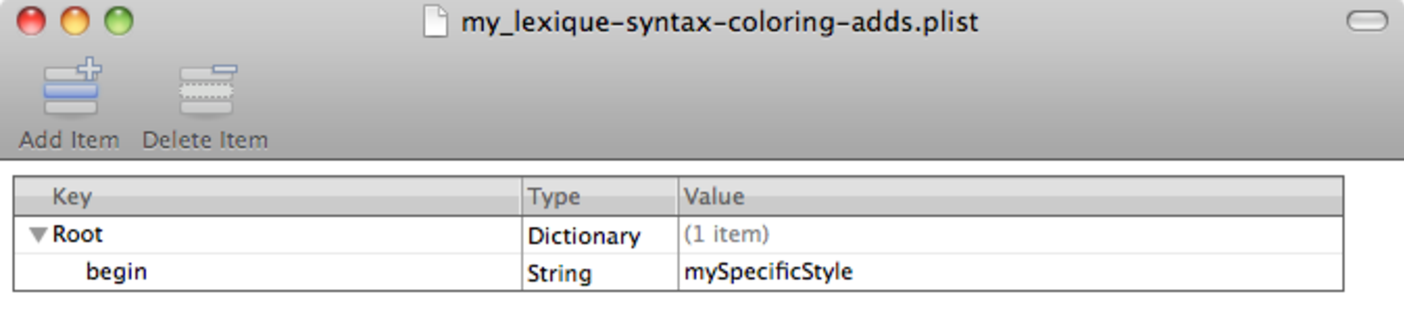
\includegraphics[width=15cm]{chapter-cocoa-features/custom-syntax-coloring-property-list-edition.pdf}
%  \caption{Example of a syntax coloring property list}
%  \labelFigure{customSyntaxColoringPropertyList}
%  \ligne
%\end{figure}
%
%If your provides an undefined style name, you will be warned every time you open a document by a beep and a small explanation window.






\sectionLabel{Indexation des fichiers sources}{indexingYourSourceFiles}

Vous pouvez configurer votre projet GALGAS pour que l'application Cocoa engendrée établisse une indexation et des références croisées : un \tpp{cmd-click} affiche un menu contextuel. Cette indexation est basée sur l'analyse syntaxique. C'est ce qui a été fait pour l'application \texttt{CocoaGalgas} (\refFigure{}{indexingUnderCocoaGALGAS}). On voit dans le menu contextuel trois classes d'index : \tpp{Class Definition}, \tpp{Class Reference as Superclass} et \tpp{Abstract Category Method Definition} ; au dessous, les références croisées correspondantes.


%You can configure your project for enabling cross-referencing entities with your Cocoa application. This has been done in GALGAS, providing such feature (\refFigure{}{indexingUnderCocoaGALGAS}). The contextual menu is displayed with a \texttt{cmd-click}.

\begin{figure}[t]
  \centering
  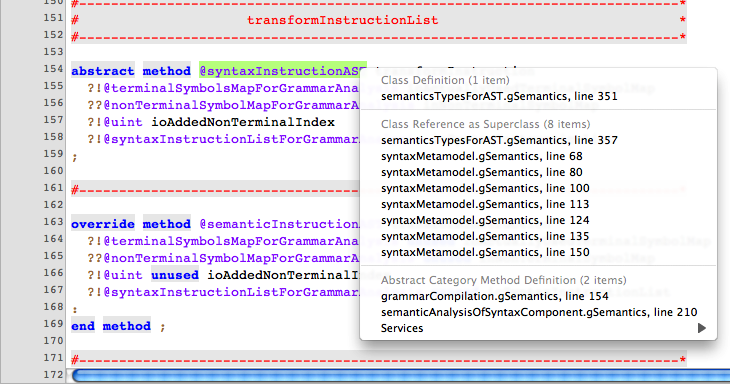
\includegraphics[width=16cm]{chapter-cocoa-features/indexing-sample.png}
  \caption{Indexation et références croisées dans l'application CocoaGalgas}
  \labelFigure{indexingUnderCocoaGALGAS}
  \ligne
\end{figure}

Pour configurer votre projet, vous avez à modifier le composant \emph{lexique}, le composant \emph{syntax}, le composant \emph{grammar}, et la règle d'analyse du fichier source. Les cinq modifications sont présentées successivement ci-après, en prenant comme exemple le langage LOGO (\refSectionPage{presentation-logo}).





\subsection{En tête du composant \texttt{lexique}}

Il faut modifier l'en-tête, en ajoutant la déclaration  \ggs+indexing in+ :


\begin{galgas}
lexique logo_lexique indexing in "INDEXING" {
  ...
\end{galgas}

La chaîne \ggs+"INDEXING"+ définit le nom du répertoire qui contient les fichiers cache de l'indexation. Ce répertoire est relatif au répertoire qui contient le fichier source.

Note : si vous effectuez maintenant la compilation GALGAS, vous obtiendrez une erreur sur la définition de la grammaire, indiquant qu'elle doit aussi indiquer la prise en compte de l'indexation.




\subsection{En tête du composant \texttt{grammar}}

Il suffit de préfixer par \ggs+indexing+ l'en-tête du composant \ggs+grammar+ :

\begin{galgas}
indexing grammar logo_grammar ... {
  ...
\end{galgas}

Note : maintenant, la compilation GALGAS s'effectue sans erreur.




\subsection{Règle d'analyse des fichiers sources}

La règle d'analyse des fichiers source doit mentionner dans l'en-tête la grammaire utilisée pour l'analyse (pour l'exemple du langage LOGO, la troisième ligne \ggs+grammar logo_grammar+ remplit ce rôle).

\begin{galgas}
case . "logo"
message "a source text file with the .logo extension"
grammar logo_grammar
?sourceFilePath:@lstring inSourceFile {
  grammar logo_grammar in inSourceFile
}
\end{galgas}

Quand le mode d'exécution (absence de l'option \tpp{-{}-mode}) est le mode par défaut, les instructions de la règle sont exécutées. Ci-dessus, la seule instruction est \ggs+grammar logo_grammar in inSourceFile+ (ligne 5).

Quand le mode d'exécution (présence de l'option \tpp{-{}-mode}) n'est pas le mode par défaut, les instructions de la règle ne sont pas exécutées, et les opérations sont guidées par la grammaire indiquée ligne 3. Dans le cas de l'indexation, l'exécution construit l'indexation du fichier source.









\subsection{Déclaration des classes d'index}

La déclaration des classes d'index s'effectue dans l'analyseur lexical. Dans la cadre du langage d'exemple LOGO, on veut simplement indéxer les routines, plus précisément l'endroit de leur définition, et les endroits où elles sont appelées. On définit donc deux classes d'index \ggs+routineDefinition+ et \ggs+routineCall+. À chaque déclaration est associée une chaîne de caractères, qui sera le titre affiché dans le menu contextuel. 


\begin{galgas}
lexique logo_lexique indexing in "INDEXING" {
  ...
indexing routineDefinition : "Routine Definition"
  ...
indexing routineCall : "Routine call"
  ...
\end{galgas}


Ces définitions peuvent être placées à tout endroit dans la définition de l'analyseur lexical.








\subsection{Définition des entrées indexées}

L'analyseur syntaxique va être complété de façon à définir les symboles qui seront indéxés. Plus précisement, c'est l'instruction d'analyse de symbole terminal qui est modifiée.

Considérons d'abord la déclaration de routine. La règle de l'analyseur syntaxique qui définit cette analyse est :

\begin{galgas}
rule <routine_definition> {
  $ROUTINE$
  $identifier$ ?let @lstring routineName
  $BEGIN$
  <instruction_list>
  $END$
}
\end{galgas}

Le nom de la routine est défini par l'instruction \ggs+$identifier$ ?let @lstring routineName+ : on la modifie alors de façon à signifier que l'indentificateur doit être indéxé comme une définition de routine :

\begin{galgas}
rule <routine_definition> {
  $ROUTINE$
  $identifier$ ?let @lstring routineName indexing routineDefinition
  $BEGIN$
  <instruction_list>
  $END$
}
\end{galgas}

Maintenant, l'instruction d'appel de routine :

\begin{galgas}
rule <instruction> {
  select
    $CALL$
    $identifier$ ?let @lstring routineName
    $;$
  or
    ...
  end
}
\end{galgas}

On modifie de manière analogue l'instruction \ggs+$identifier$ ?let @lstring routineName+ :

\begin{galgas}
rule <instruction> {
  select
    $CALL$
    $identifier$ ?let @lstring routineName indexing routineCall
    $;$
  or
    ...
  end
}
\end{galgas}



\subsection{Compilation et essai}

Les modifications sont terminées. Vous pouvez recompiler votre projet (compilation GALGAS puis compilation de la cible Cocoa du projet \texttt{Xcode}). La \refFigure{}{exemple-indexation-logo} montre le résultat obtenu en effectuant un \tpp{cmd-click} sur le nom de la routine.

\begin{figure}[t]
  \centering
  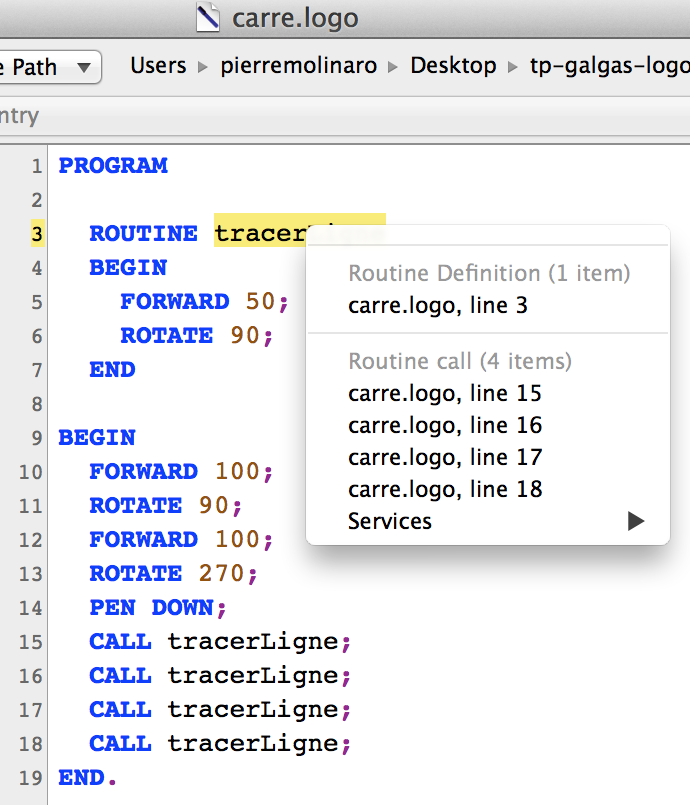
\includegraphics[width=8cm]{chapter-cocoa-features/exemple-indexation-logo.png}
  \caption{Exemple d'indexation en LOGO}
  \labelFigure{exemple-indexation-logo}
  \ligne
\end{figure}



%\noindent{4} \textbf{Program component configuration.} Insert the \ggs+grammar+ declaration after the « \texttt{message ...} » declaration in every program rule concerned by indexing:
%
%\begin{galgas}
%case ...
%message ...
%grammar my_grammar
%?@lstring inSourceFile {
%  ...
%\end{galgas}
%
%
%
%
%
%
%\noindent{5} \textbf{Define indexing entries.} The indexing entries are defined within the rules of syntax components. The \emph{terminal check} instruction is the unique way for definition, by naming an index class name:
%
%\begin{galgas}
%syntax ... ("my_lexique.gLexique") :
%  ...
%rule ... :
%  ...
%  $identifier$ ? ... indexing myIndexClass1 ;
%  ...
%end rule ;
%  ...
%\end{galgas}
%
%Any kind of terminal symbol accepts an « \texttt{indexing} » attribute : keywords, delimiters, literal string, integers, identifiers, \dots
%
%Several index class names can be named, using a comma as separator:
%\begin{galgas}
%  ...
%  $identifier$ ? ... indexing myIndexClass1, myIndexClass2 ;
%  ...
%\end{galgas}
%
%
%
%
%
%
%\noindent{6} \textbf{Compile and play.} Now, you can compile and run the Cocoa Application. With a \texttt{cmd}-click on an indexed terminal symbol, the contextual menu is displayed. You can delete the indexing directory at any moment, it will be rebuilt as needed.










%-----------------------------------------------------------------------------------------------------------------------*
%                                                                                                                       *
%   I N D E X                                                                                                           *
%                                                                                                                       *
%-----------------------------------------------------------------------------------------------------------------------*

\cleardoublepage % Pour commencer a une page impaire
\phantomsection  % Pour faire correctement pointer l'hyperlien dans la table des matières

%--- Ecrire l'index
{\small
\printindex
}

%-----------------------------------------------------------------------------------------------------------------------*
%                                                                                                                       *
%   F I N    D U    D O C U M E N T                                                                                     *
%                                                                                                                       *
%-----------------------------------------------------------------------------------------------------------------------*

\end{document}

%-----------------------------------------------------------------------------------------------------------------------*

